\documentclass[12pt, oneside, a4paper]{ctexart}
\usepackage{amsmath}
\usepackage{amssymb}
\usepackage{caption}
\usepackage{ctex}
\usepackage{enumerate}
\usepackage{float}
\usepackage{tocloft}
\usepackage[{top=2.54cm, bottom=2.54cm, left=3.18cm, right=3.18cm}]{geometry}
\usepackage{graphicx}
\usepackage[breaklinks, colorlinks=false, hidelinks]{hyperref}
\usepackage{mathptmx}
\usepackage{xcolor}
\usepackage{xeCJK}

\ctexset{
    section={   
        name={,、},
        number={\heiti\chinese{section}},
        format=\heiti\raggedright\zihao{3}\bfseries,
        aftername={\hspace{0.5em}},
        beforeskip=1ex,
        afterskip=1ex,
    },
    subsection={
        name={,.},
        number={\arabic{section}.\arabic{subsection}},
        format=\songti\raggedright\zihao{4}\bfseries,
        aftername={\hspace{0.5em}},
        beforeskip=0ex,
        afterskip=0ex,
    },
    subsubsection={
        name={,.},
        number={\arabic{section}.\arabic{subsection}.\arabic{subsubsection}},
        format=\songti\raggedright\zihao{-4}\bfseries,
        aftername={\hspace{0.5em}},
        beforeskip=0ex,
        afterskip=0ex,
    },
}
\setlength{\cftbeforesecskip}{1ex plus 0.1ex}
\setlength{\cftbeforesubsecskip}{0ex plus 0.05ex}
\setlength{\cftbeforesubsubsecskip}{0ex plus 0.05ex}
\pagestyle{plain}
\renewcommand{\figurename}{\small{图}}
\setmainfont{Times New Roman}
\setCJKmainfont[AutoFakeBold={2}]{SimSun}
\setCJKfamilyfont{zh}{SimSun}
\setCJKfamilyfont{ja}{BIZ UDMincho}
\xeCJKDeclareCharClass{CJK}{
  "24EA,
  "2460->"2473,
  "3251->"32BF,
  "24FF,
  "2776->"277F,
  "24EB->"24F4
}



%----------分割线----------%



\begin{document}



\thispagestyle{empty}
\begin{center}{
    \fontsize{26pt}{26pt}\selectfont
    \vspace*{2.75\baselineskip}
    
\includegraphics[width=0.6\textwidth]{pics/tongji-university-logo-1024px.png}\\
    [\baselineskip]
    \heiti{轨道车辆设计作业（一）}\\
    \fontsize{18pt}{24pt}\selectfont
    \vspace*{2\baselineskip}
    \songti{\begin{tabular}{l}
            {\heiti{}完成日期：}2026年5月26日 \\
            {\heiti{}报告作者：}肖哲夫~~2352670
        \end{tabular}
        \vspace{0.25cm}
        \\\textcolor{gray}{\textit{Made with }\LaTeX}}
    }
\end{center}
\newpage{}
\setcounter{page}{1}
{
    \heiti{}
    \renewcommand{\contentsname}{\makebox[\textwidth][c]{\zihao{2}\heiti\textbf{目录}}}
    \tableofcontents
}
\newpage{}
\setcounter{page}{1}
\section{\heiti{概述}}
\par{}
本次作业旨在练习个人使用HyperMesh等软件进行有限元仿真的能力，以日常生活中的某一产品为对象，对其进行静态特性分析、动态特性分析、稳定性分析、结构优化分析、疲劳分析、冲击耐碰撞分析等。
\par{}
其中，选择的分析对象为手工制作的木制折叠梯，在SOLIDWORKS中进行建模后，根据实际情况进行简化，再导入HyperMesh中进行前处理，使用Optistruct进行求解，最后在HyperView中进行后处理和结果分析。
\par{}
\quad{}
\par{}
\section{\heiti{SOLIDWORKS建模与简化}}
\subsection{\heiti{SOLIDWORKS建模}}
\par{}
在SOLIDWORKS~2020中进行建模，图1为折叠梯渲染图，该折叠梯主要由5部分组成：顶板（供站立）、前支撑（含Z字形部件）、后支撑（含梯级）和左右连接件。其中各部分内部的部件采用$\rm 5 \times 28~mm$木制暗榫固接，各部分之间采用$\rm M6 \times 45~mm$或$\rm M6 \times 55~mm$钢制螺栓（配螺母、垫圈）连接，可以转动；每侧四个螺栓作为一个关节，恰好构成一个四杆连杆机构，实现折叠梯的折叠收纳功能。
\par{}
\begin{figure}[htbp]
    \centering
    \vspace{-0.3cm}
    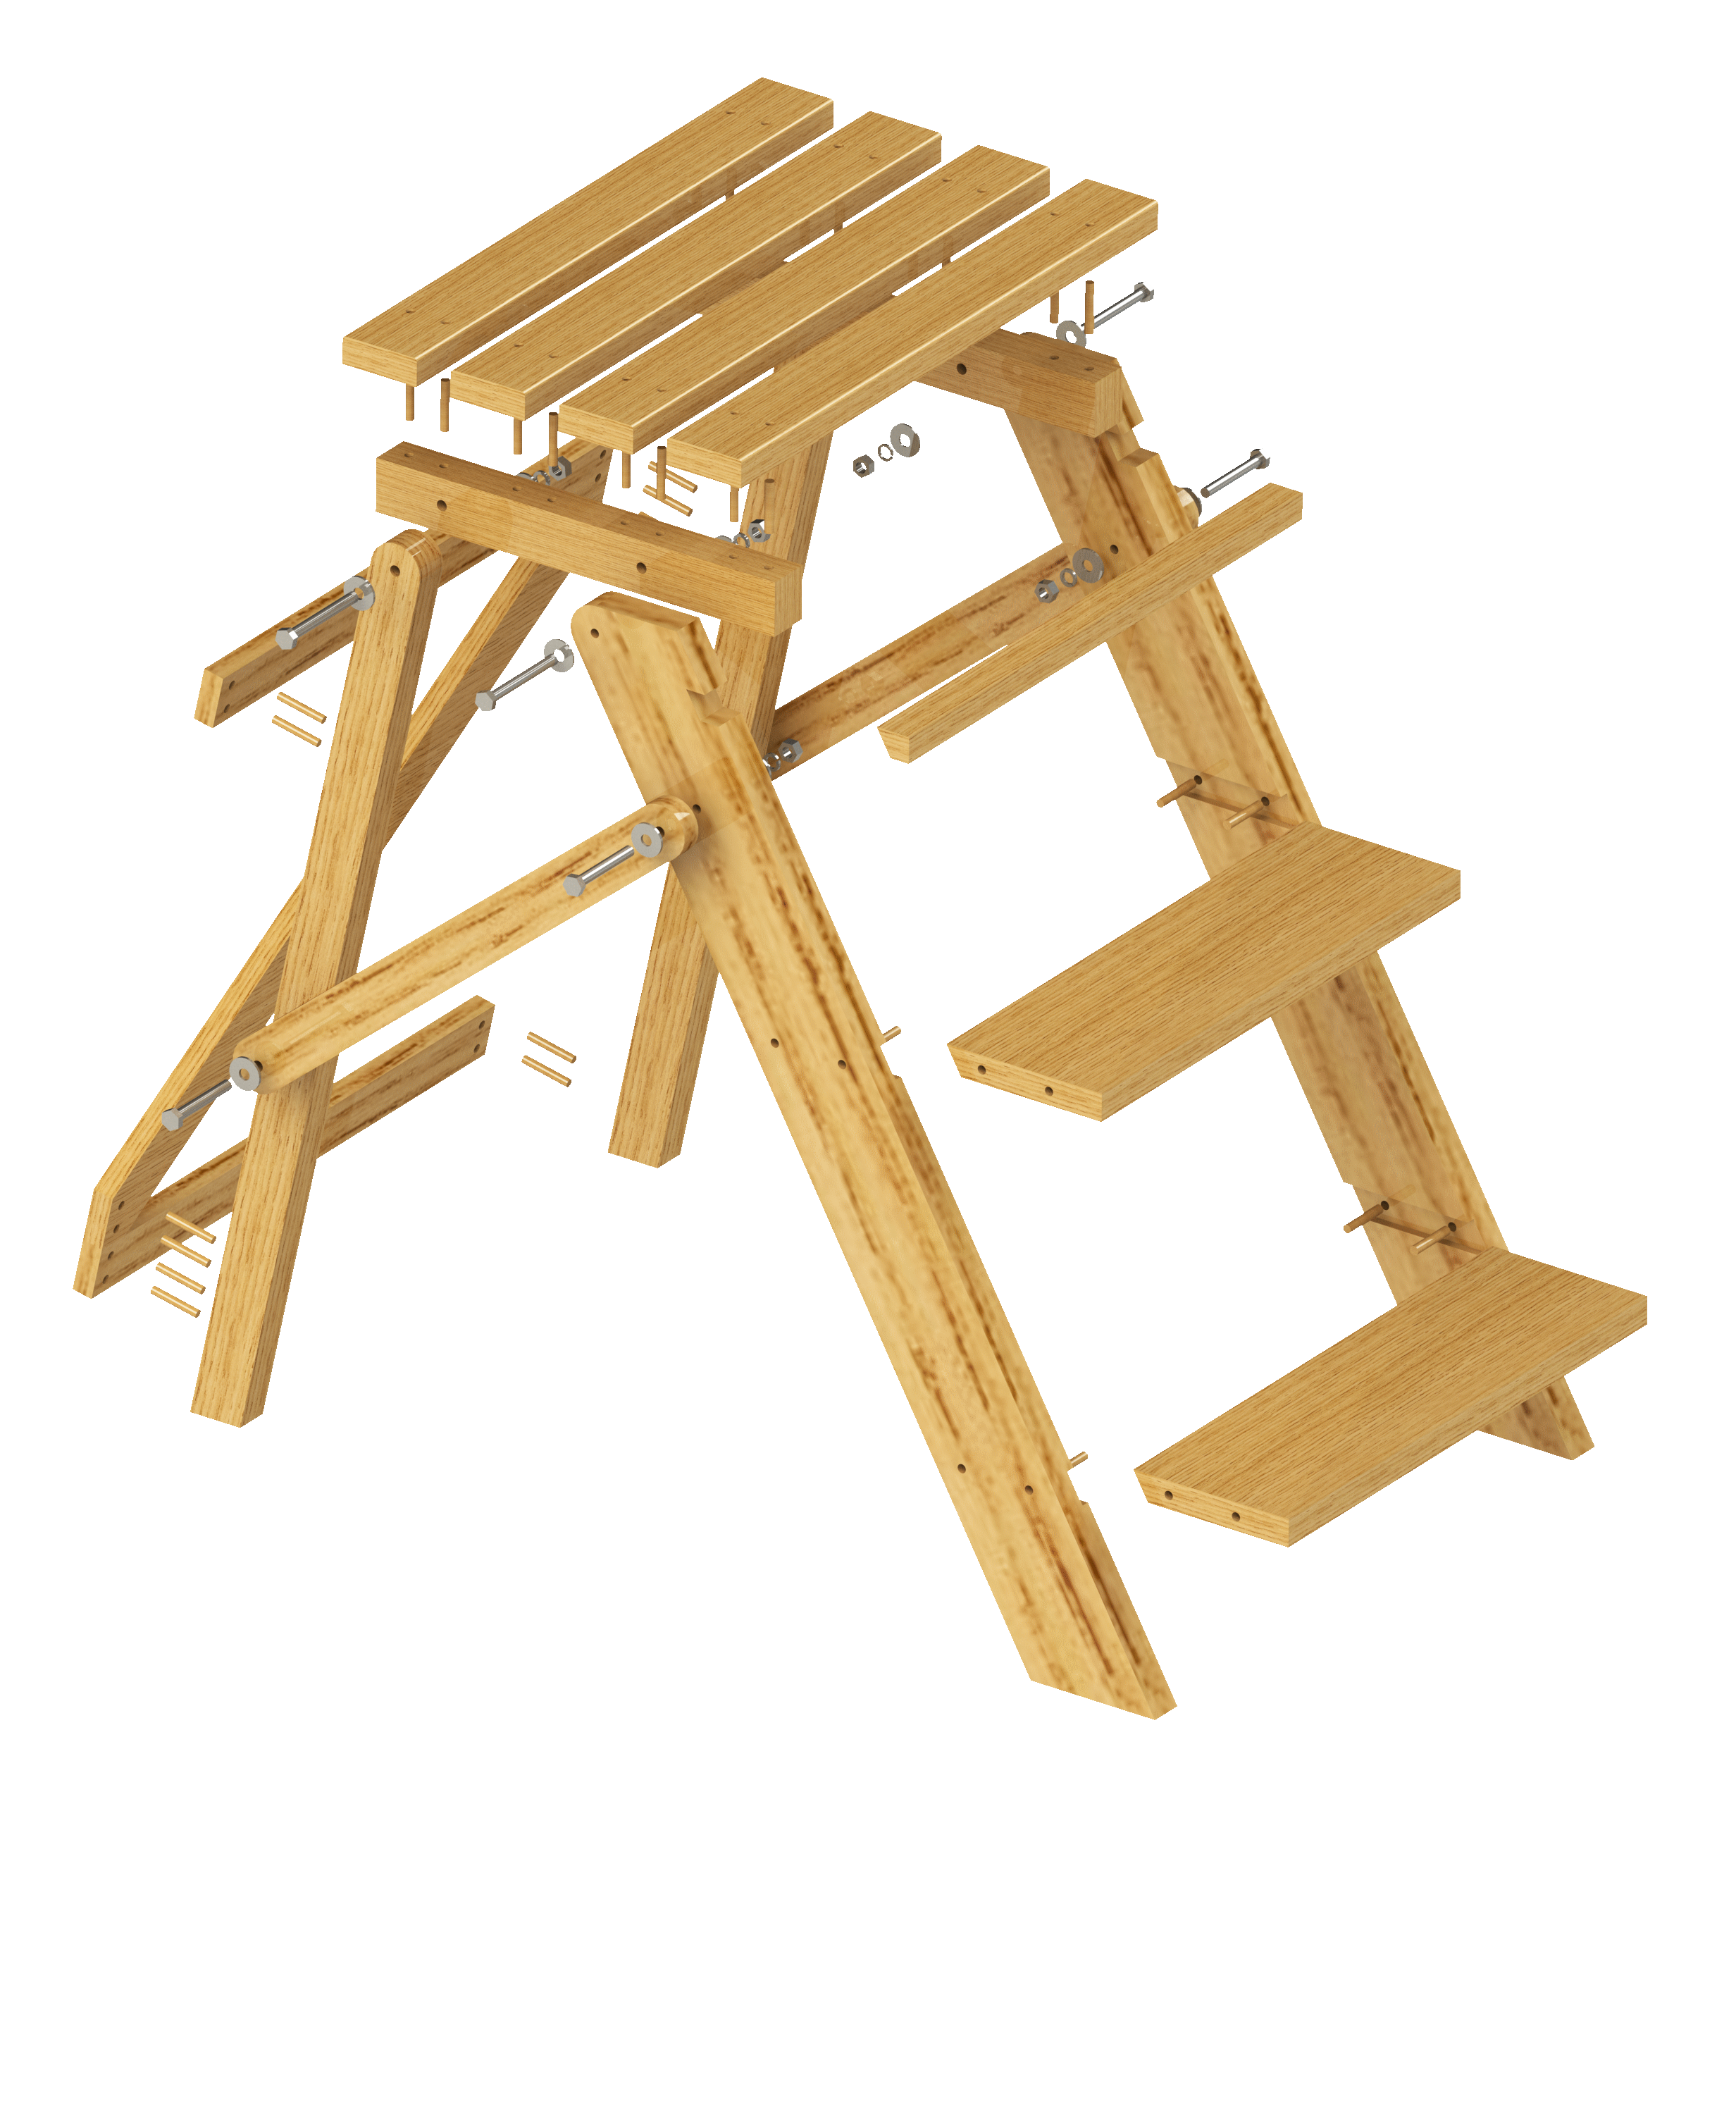
\includegraphics[height=6cm]{pics/01_LADDER_EXPLD_RENDERED.png}
    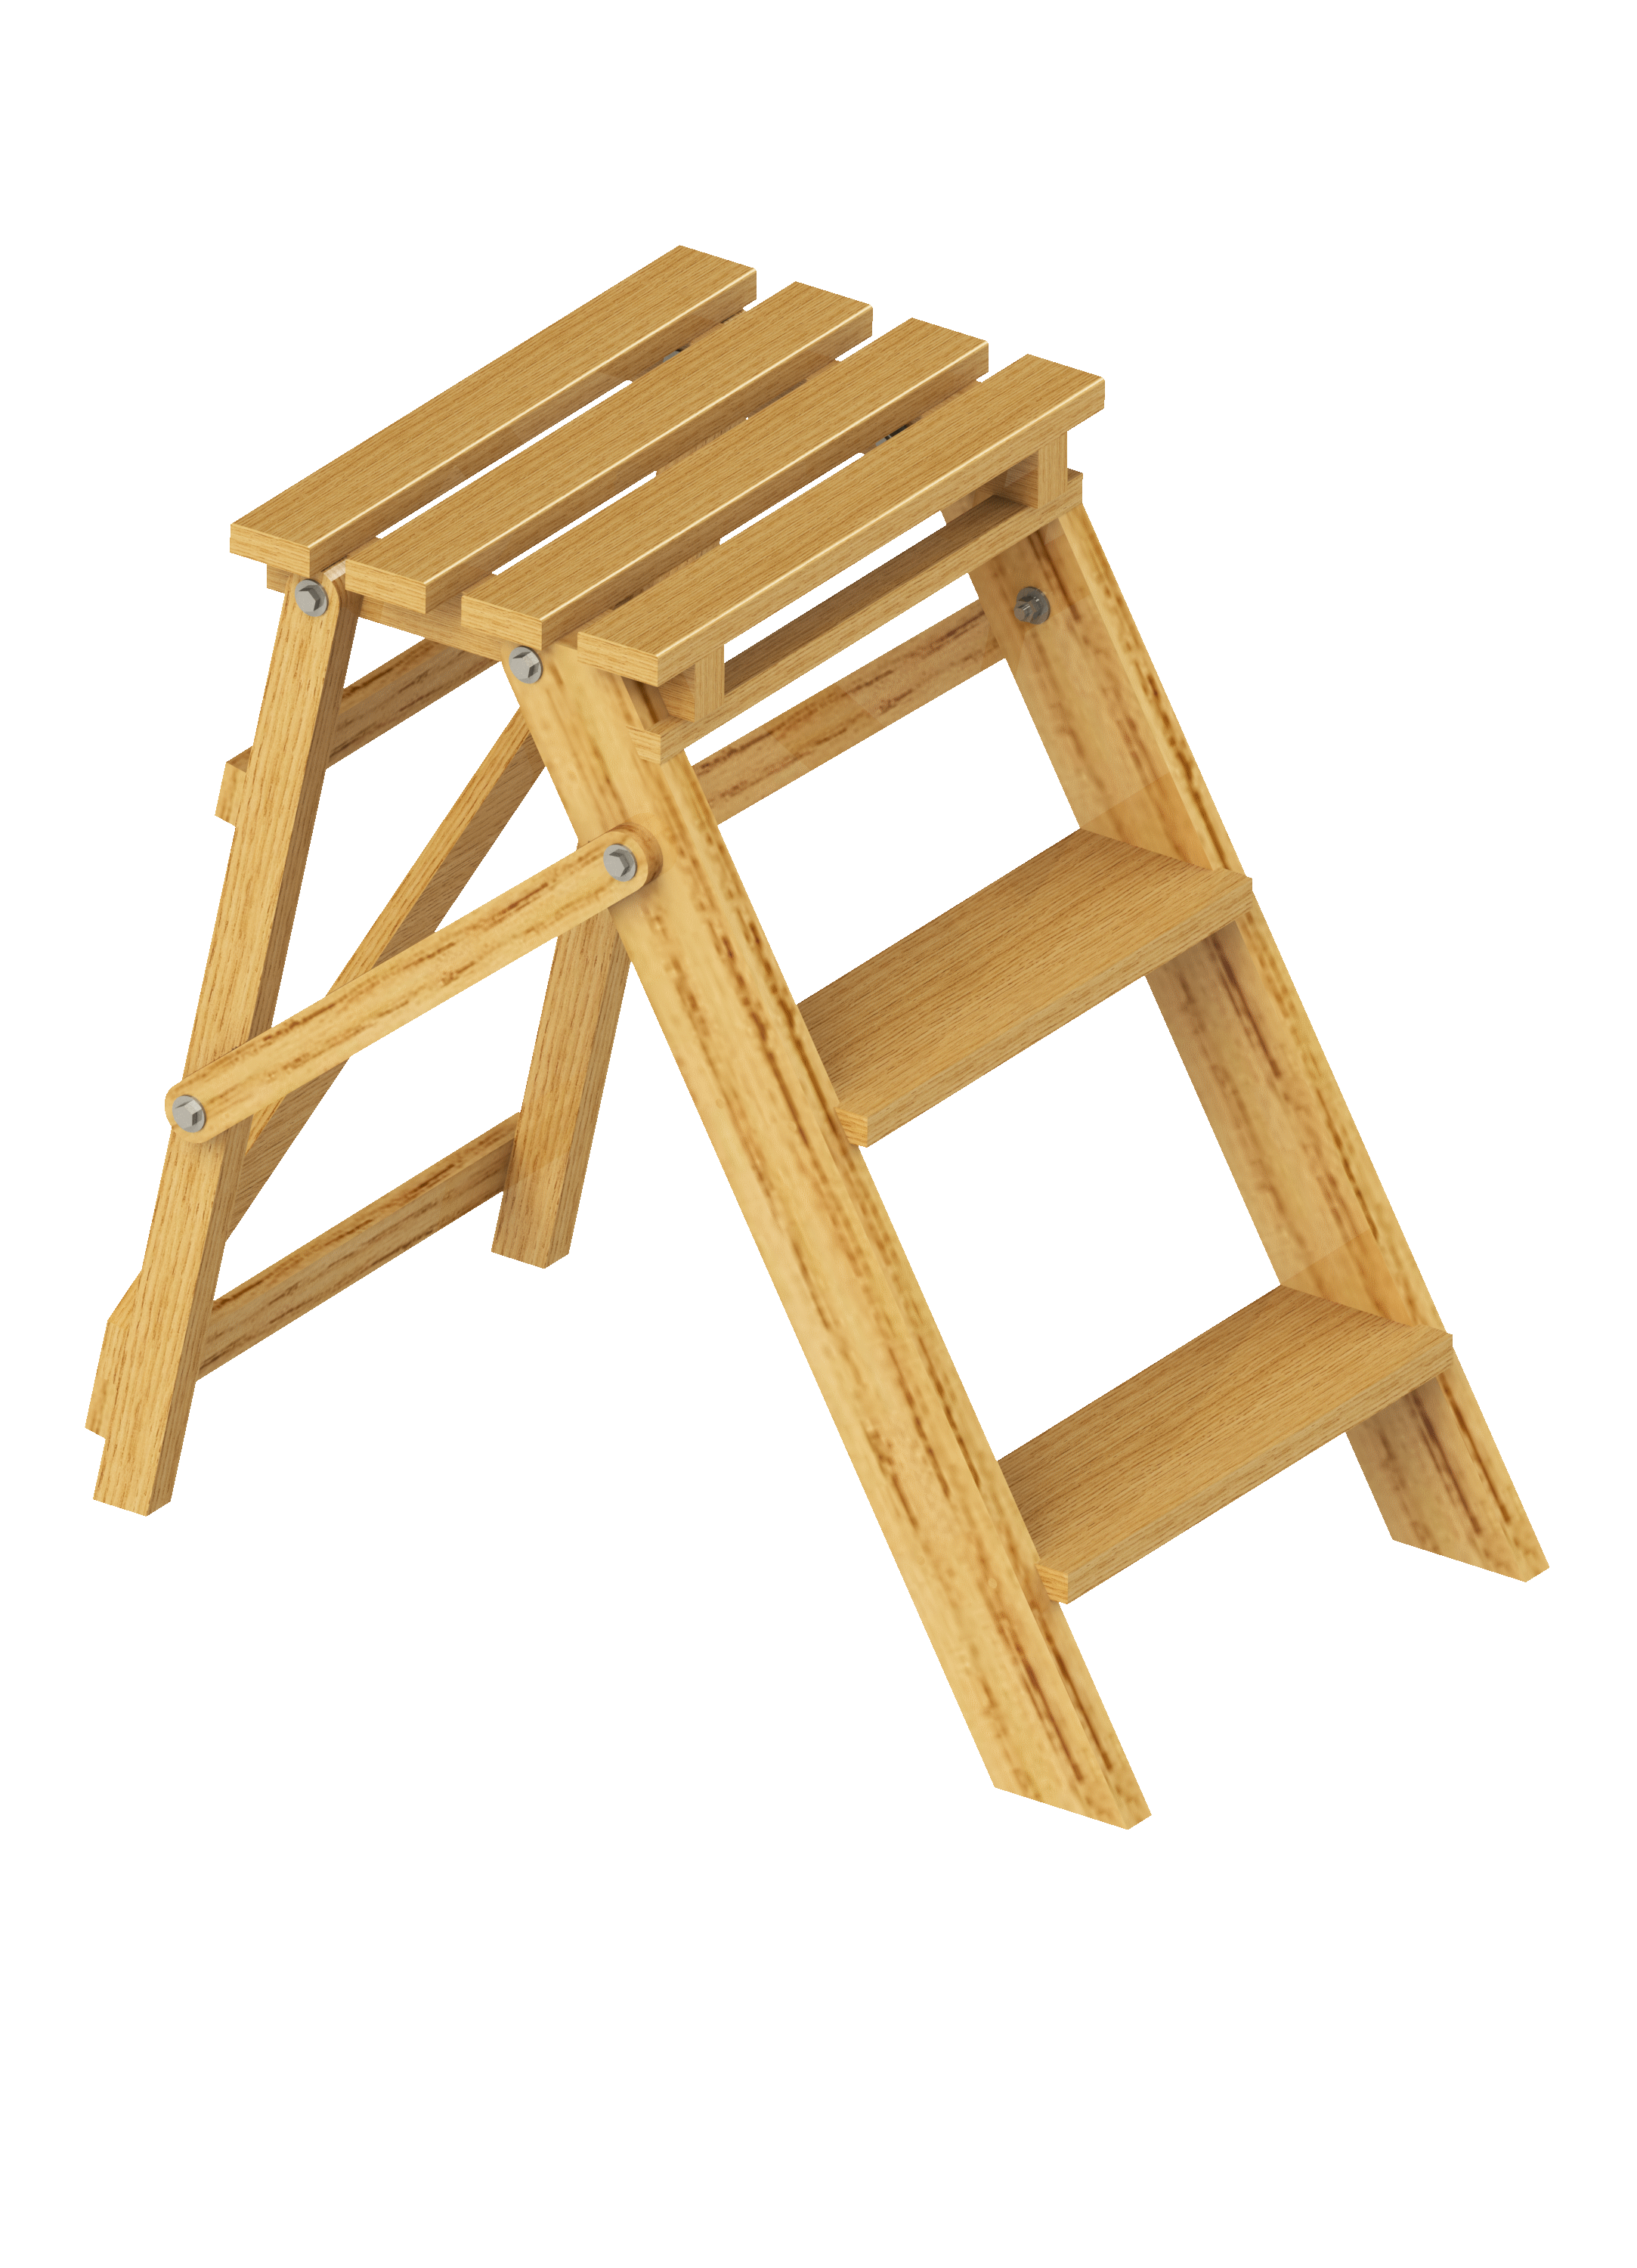
\includegraphics[height=6cm]{pics/01_LADDER_RENDERED.png}
    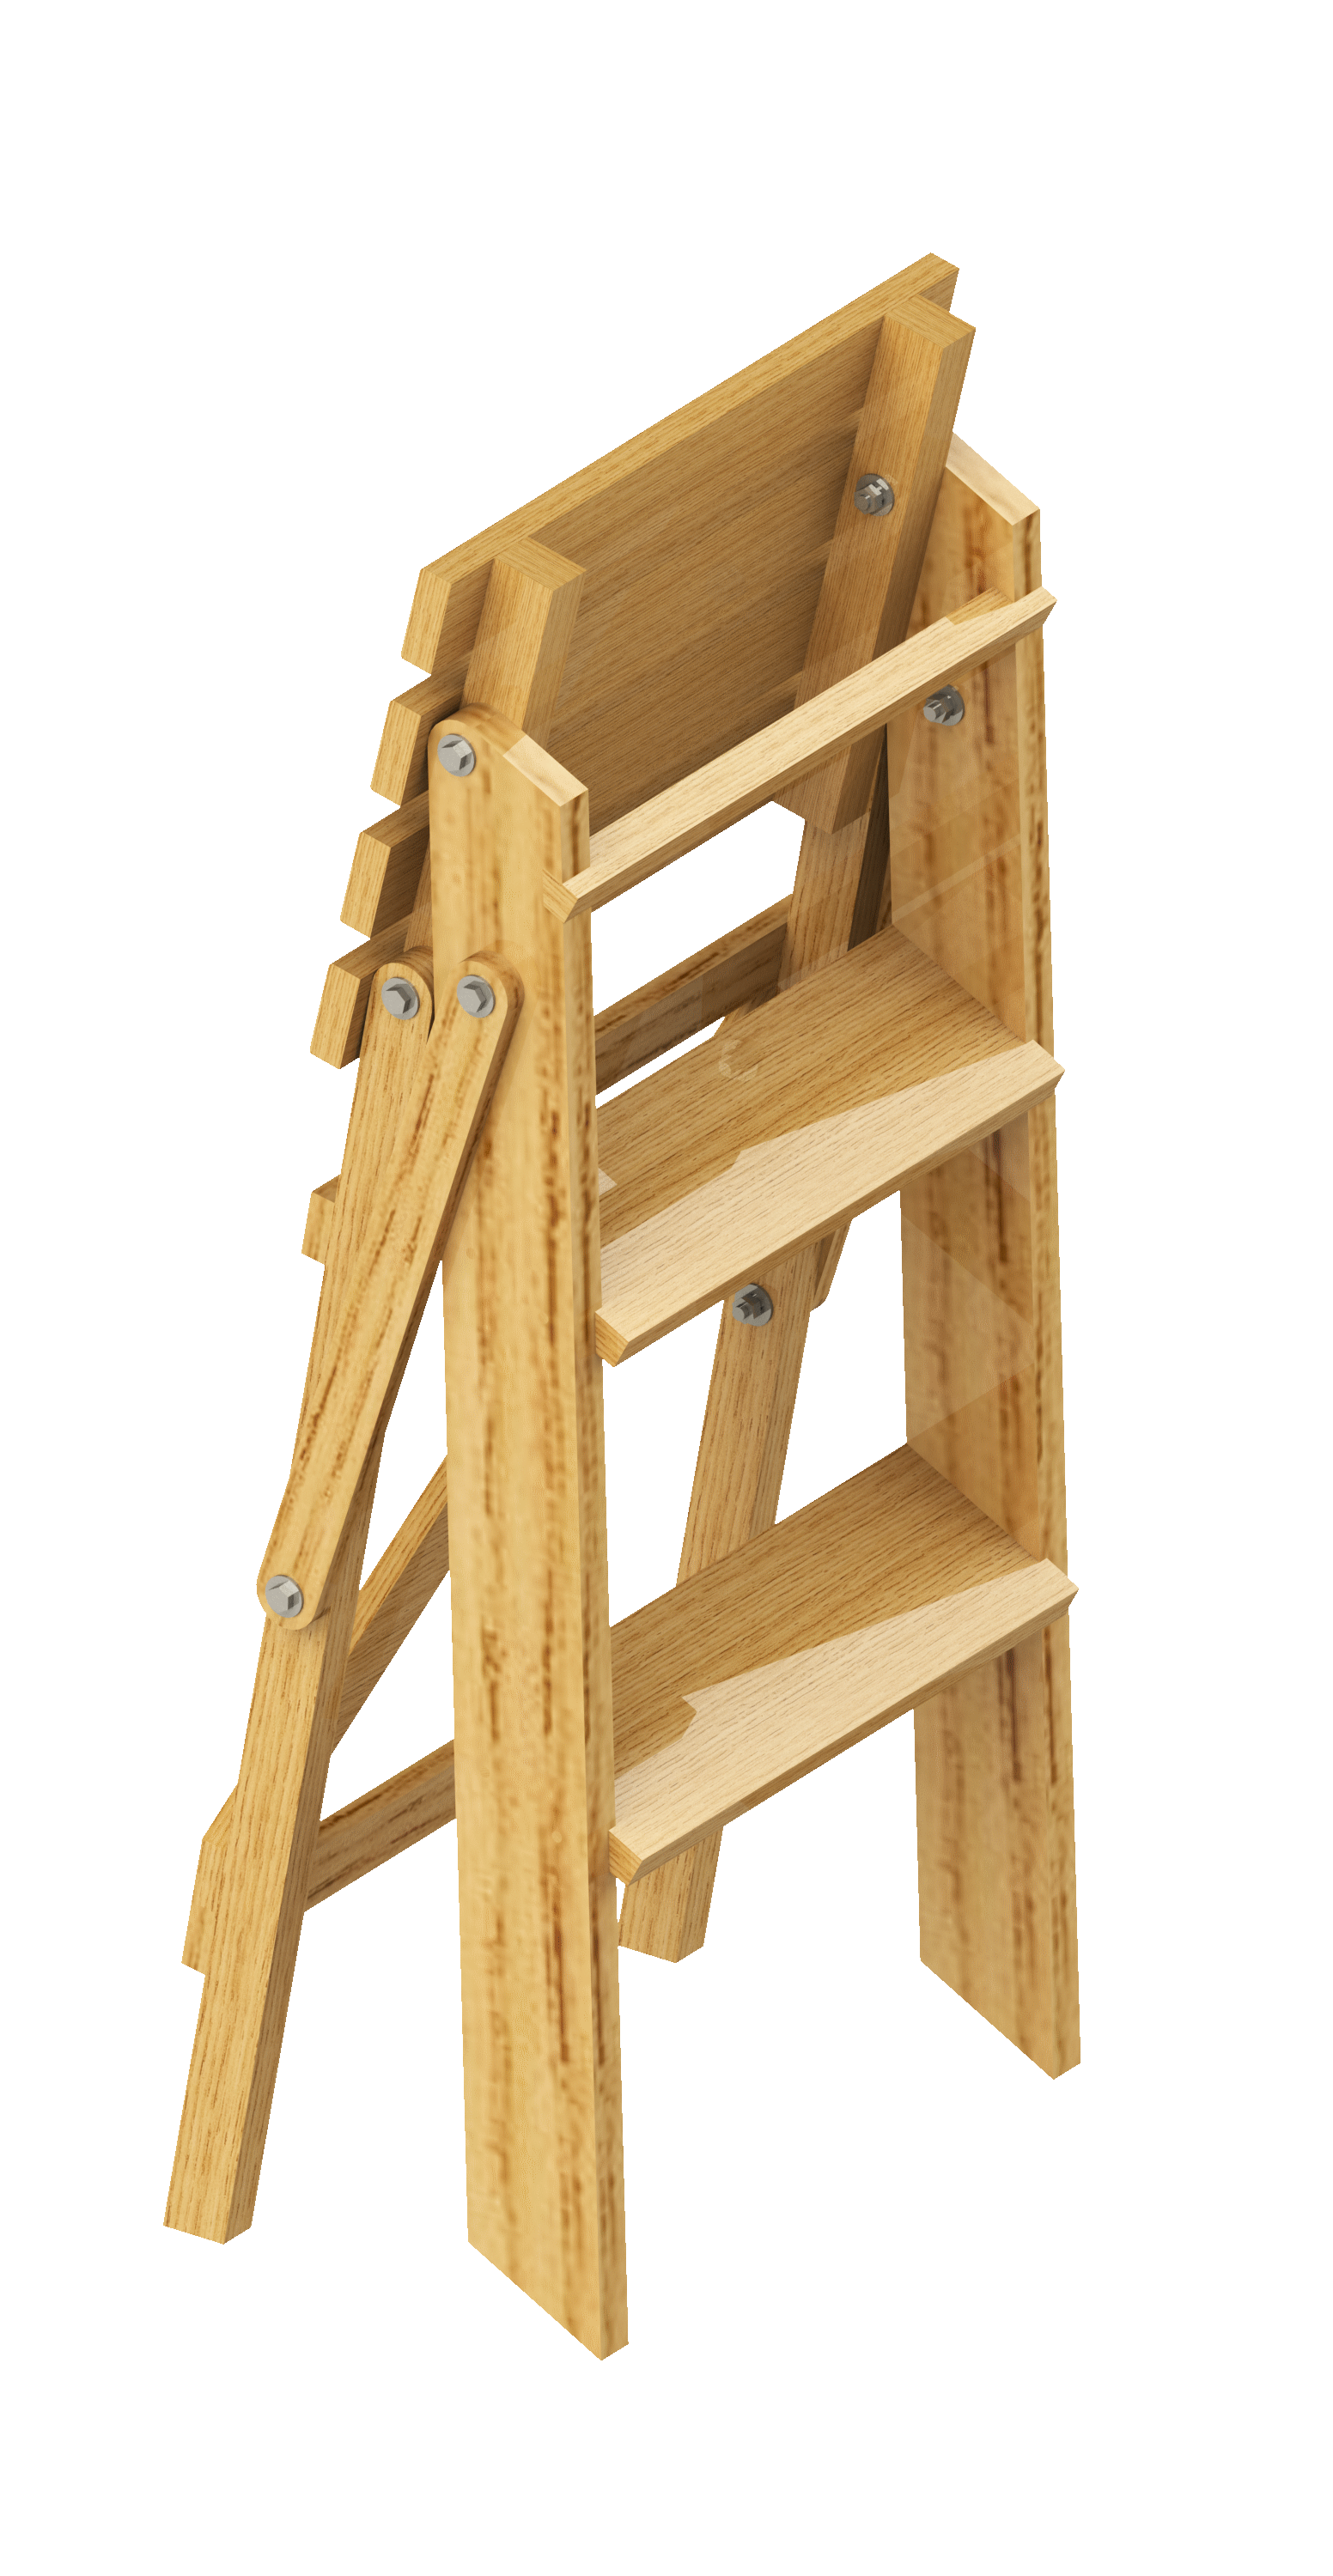
\includegraphics[height=6cm]{pics/01_LADDER_FOLDED_RENDERED.png}
    \vspace{-1.1cm}
    \caption{\small{折叠梯渲染图}}
    \vspace{-0.4cm}
\end{figure}
\subsection{\heiti{模型简化}}
\par{}
日常使用时，折叠梯主要处于展开状态，人站在梯级踏板或顶板上，承载力主要通过螺栓与木制大块部件传导，木制暗榫几乎仅起到非受力方向的固定作用、不参与传力；螺栓形变较小且几乎完全满足应力要求；实体螺栓会增加计算负担。因此，对模型作如下简化：各部分内部采用暗榫连接的，包括暗榫在内直接视作一个整体做分析；又因为顶板和后支撑的受力主要通过连接件与后支撑顶面传导，且两者之间始终紧密贴合，同时为了防止有限元分析时因两者接触导致的网格穿透，故在模型中将两者直接视为整体进行分析；钢制螺栓等在前处理软件HyperMesh中进行理想化处理。因此最终模型包括前支撑、后支撑与顶板组合体、左右连接件共4块。
\newpage{}
\section{\heiti{有限元模型介绍}}
\subsection{\heiti{模型导入}}
\par{}
将简化合并后的模型在SOLIDWORKS中另存为.STEP文件，并打开Altair HyperWorks 2026，选择启动HyperMesh，点击“File~→~Import~→~Geometry Model”，选择默认设置直接导入模型。如图2所示，导入后测量顶板宽度为360，刚好匹配实际尺寸360~mm；检查设置“File~→~Preferences~→~搜索‘Unit’”，得单位制为MMKS，说明模型尺寸正确。
\par{}
\begin{figure}[htbp]
    \centering
    \vspace{-0.3cm}
    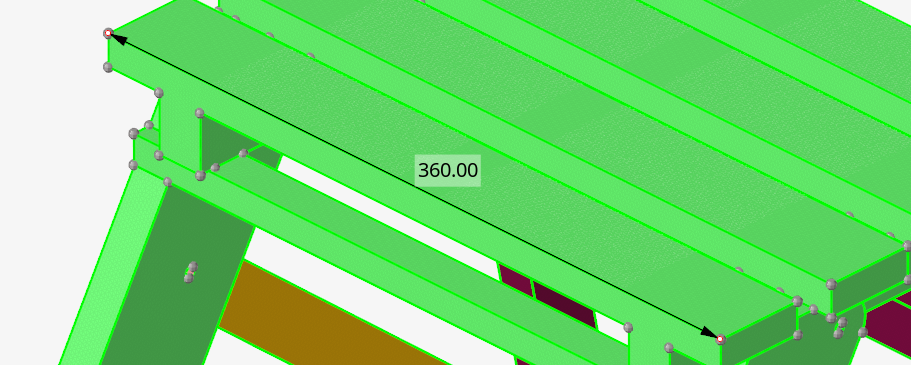
\includegraphics[height=3cm]{pics/02_Measurement.png}
    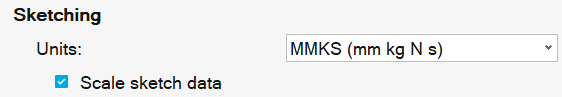
\includegraphics[height=1cm]{pics/02_Unit.png}
    \vspace{-0.4cm}
    \caption{\small{尺寸检查}}
    \vspace{-0.4cm}
\end{figure}
\subsection{\heiti{模型网格划分}}
\par{}
点击“3D~→~Tet”进入四面体网格划分界面，先选中一个实体（Solid）并设置网格大小为2，直接点击“Mesh”进行网格划分。一个实体的网格划分完成后再划分下一个实体，以避免软件卡顿。最终得到的三维网格/元素（3D~Elements）数量为约441.9万、节点（Nodes）数量为约86万，如图3。
\par{}
\begin{figure}[htbp]
    \centering
    \vspace{-0.3cm}
    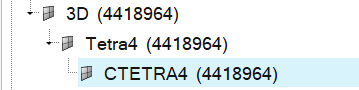
\includegraphics[height=1cm]{pics/03_El.png}
    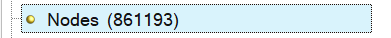
\includegraphics[height=0.425cm]{pics/03_No.png}
    \vspace{-0.4cm}
    \caption{\small{四面体网格数与节点数}}
    \vspace{-0.4cm}
\end{figure}
\par{}
本人也尝试划分六面体网格，虽然更为整齐美观，但由于模型较为复杂，六面体网格划分需要更多的人工切割，且很容易导致网格质量下降（不满足默认网格质量要求的网格占比约为2.3\%，较难手动修复），因此最终仍然选择四面体网格进行分析。
\subsection{\heiti{网格质量检查}}
\begin{figure}[htbp]
    \centering
    \begin{minipage}[t]{0.48\textwidth}
        \vspace{0pt}
        \par{}\qquad{}
        首先点击“Validate~→~Penetration”全选部件（Components）检查网格穿透，显示“No intersections or penatrations are found”说明不存在网格穿透问题。
        \par{}\qquad{}
        再点击“Face Color~→~Element Quality~→~3D”，检查网格质量。默认网格质量要求如图4，不合格网格数为165，占总数的约0.04\textperthousand，软件中四舍五入为0。经检查，这些网格不在受力关键区域，说明网格质量较好、无需修复。
    \end{minipage}
    \hfill
    \begin{minipage}[t]{0.48\textwidth}
        \vspace{0pt}
        \centering
        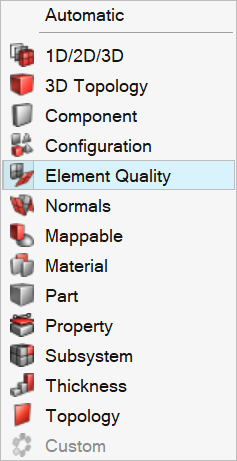
\includegraphics[height=5.5cm]{pics/04_Ch.png}
        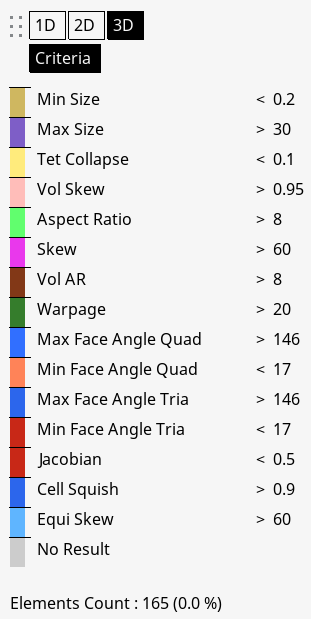
\includegraphics[height=6cm]{pics/04_Q.png}
        \vspace{-0.4cm}
        \caption{\small{网格质量检查}}
    \end{minipage}
    \vspace{-0.4cm}
\end{figure}
\newpage{}
\section{\heiti{材料选择}}
\subsection{\heiti{建立属性库}}
\par{}
针对木制部件与虚拟螺栓，分别建立属性（Properties）。其中，由于木制部件采用实体仿真，故属性为PSOLID；由于虚拟螺栓采用刚性连接，无需设置属性，只需设置连接关系。
\subsection{\heiti{建立材料库}}
\par{}
对于木制部件，由于设计文档中提到：“为确保梯子坚固，我们建议使用硬木（桦木、橡木……）和钢制紧固件\textsuperscript{\textcolor{red}{\cite{ref1}}}”，故采用松木作为主材。
\par{}
松木为各向异性材料，即不同方向上力学性质，如弹性模量等不同。因此，设置主材类型为MAT9OR；以《中华人民共和国国家标准~-~木结构设计标准》（GB~50005-2017）中附录D.2表D.2.1规定的进口北美地区目测分级规格材强度设计值和弹性模量\textsuperscript{\textcolor{red}{\cite{ref2}}}为基础进行估算，设置松木的材料属性如图5所示；再对实体的质量（Mass）进行检查，点击“Validate~→~Mass~→~Compute”计算得总质量如图5，约为$\rm 3.30~kg$，符合生活认知。
\par{}
\begin{figure}[htbp]
    \centering
    \vspace{-0.1cm}
    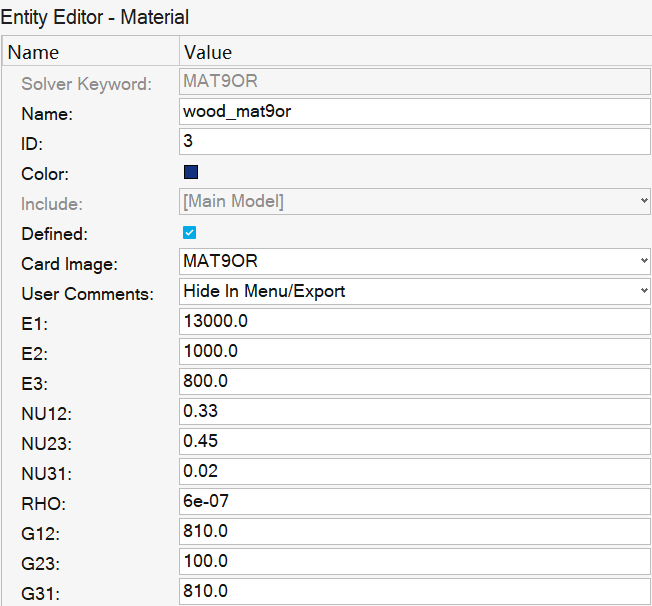
\includegraphics[height=7cm]{pics/05_MAT.png}\\
    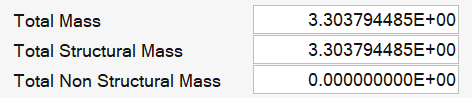
\includegraphics[height=1.25cm]{pics/05_Mass.png}
    \vspace{-0.4cm}
    \caption{\small{模型材质与总质量}}
    \vspace{-0.4cm}
\end{figure}
\par{}
\quad{}
\par{}
由于材质为各向异性，因此应将每个部件的各元素通过“Assembly~→Organize”按部件各组分的顺纹方向不同拆分成不同子部分，并将每个部分的长边方向视为顺纹方向，并设定为$x$坐标轴方向、再按各自的相对坐标系赋予不同（仅坐标系方向不同）的属性。最终属性划分结果如图6。
\clearpage
\newpage{}
\par{}
\begin{figure}[H]
    \centering
    \vspace{-0.1cm}
    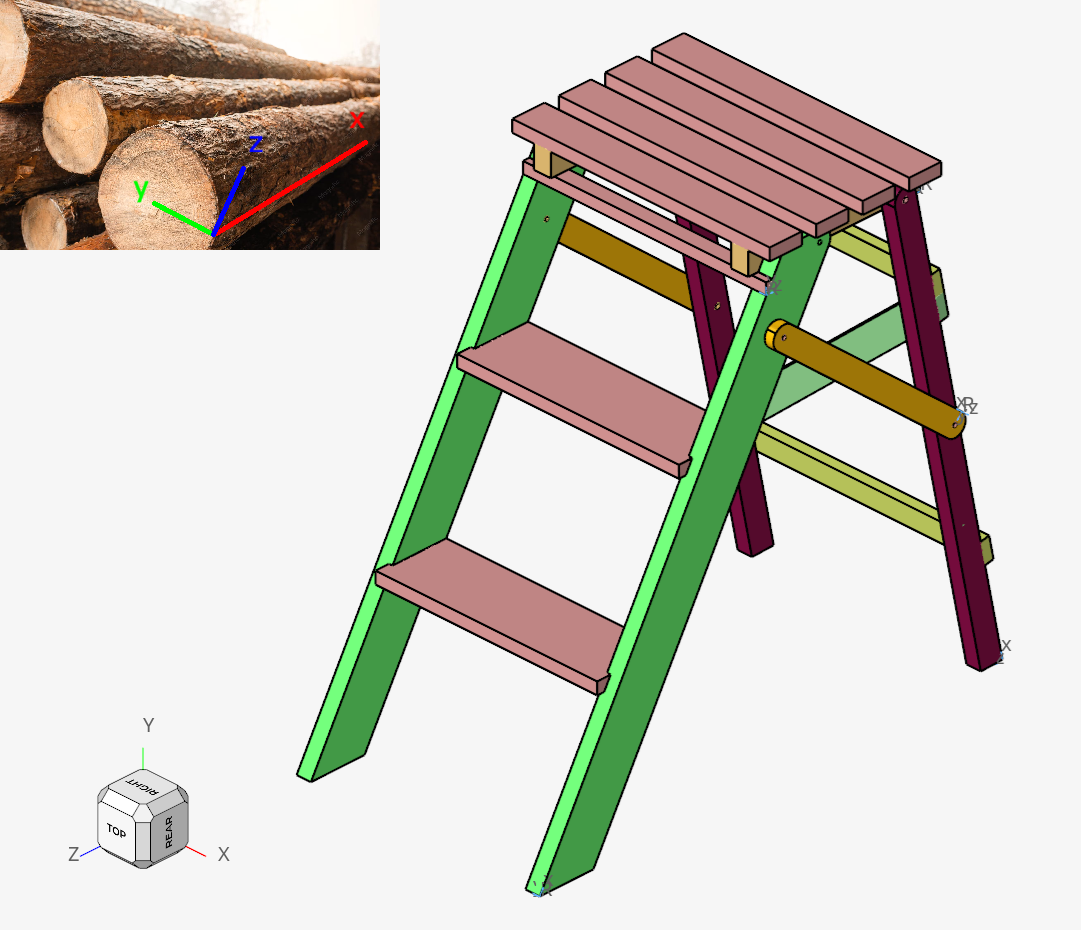
\includegraphics[height=8cm]{pics/06_Prop.png}
    \vspace{-0.4cm}
    \caption{\small{属性划分结果}}
    \vspace{-0.4cm}
\end{figure}
\clearpage
\newpage{}
\section{\heiti{工况载荷介绍}}
\subsection{\heiti{约束设置}}
\subsubsection{\heiti{边界条件设置}}
\par{}
折叠梯呈展开状态且上有稳定载荷时，底部与地面紧密贴合，且由于摩擦力，底部相对地面不会发生滑移。因此模型中可将折叠梯前后支撑底面的三个坐标平动自由度（即$x$、$y$、$z$轴平动）均设置为固定；而由于折叠梯底面有多点在$x$、$z$轴平动方向被约束，因此折叠梯整体在绕$y$轴的旋转自由度被自动约束；而考虑到实际使用中的侧滚倾覆，绕$x$、$z$轴的旋转自由度是没有被主动约束的，但同$y$轴的旋转自由度一样，它们也因为平动自由度而被自动约束了。点击“Analyze~→~Constraints”设置约束，结果如图7。
\par{}
\begin{figure}[htbp]
    \centering
    \vspace{-0.1cm}
    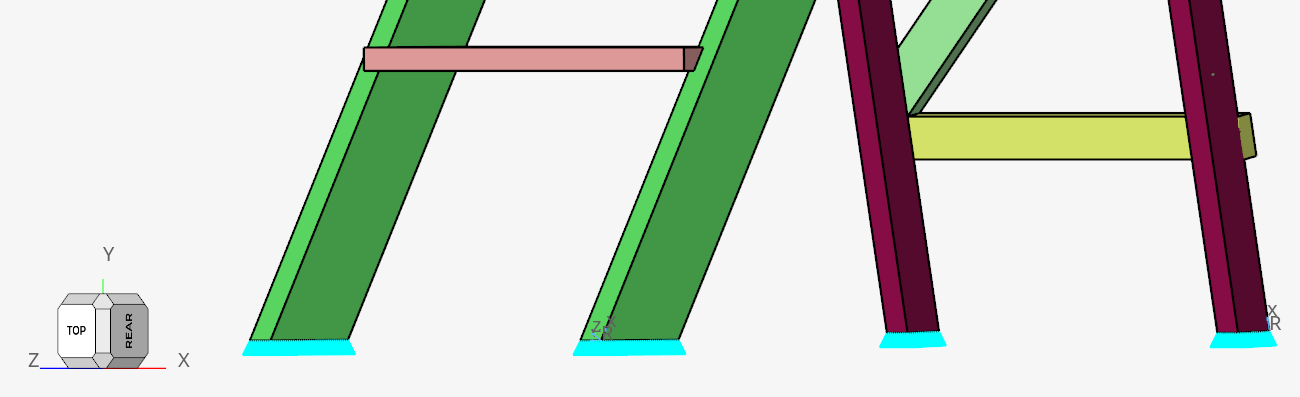
\includegraphics[width=0.75\linewidth]{pics/07_SPC.png}\\
    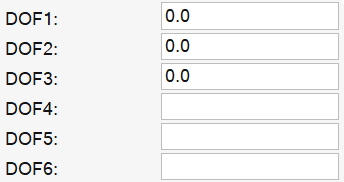
\includegraphics[width=0.2\linewidth]{pics/07_SPC_Panel.png}
    \vspace{-0.4cm}
    \caption{\small{边界条件示意图}}
    \vspace{-0.4cm}
\end{figure}
\subsubsection{\heiti{螺栓约束设置}}
\par{}
折叠梯的螺栓连接处的摩擦力可忽略，仅靠螺栓剪切应力或轴向应力传递载荷，且本算例中暂且不考虑螺栓本身受力，因此直接点击“Model~→~Rigids”采用RBE2单元将各可动关节处刚性相连，如图8。也可采用RBE3（非刚性），但需要设定螺栓材质，这里为了简化分析，直接采用RBE2。
\par{}
\begin{figure}[htbp]
    \centering
    \vspace{-0.1cm}
    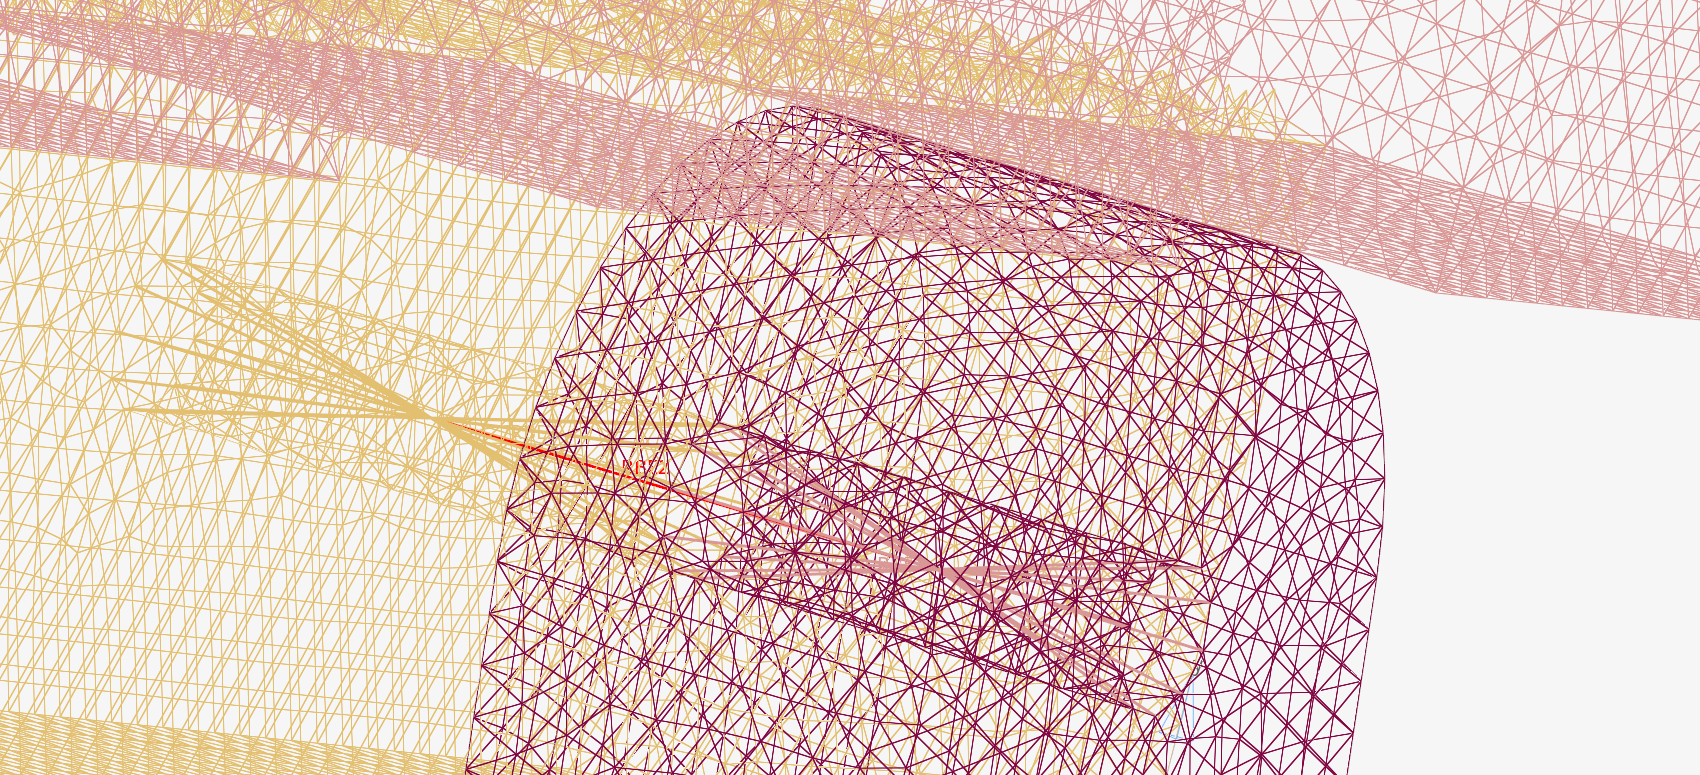
\includegraphics[width=0.5\linewidth]{pics/08_Bolts.png}
    \vspace{-0.4cm}
    \caption{\small{螺栓连接示意图}}
    \vspace{-0.4cm}
\end{figure}
\subsubsection{\heiti{接触设置（此算例中未生效，仅作练习用）}}
\par{}
根据多次仿真结果，发现尤其是顶面受载荷且螺栓设置为RBE3时，前支撑与顶板之间存在较明显的网格穿透，因此在两者之间设置接触面（Contact Surfaces）。点击“Model~→~Contact Surfaces”进入接触设置界面，选择前支撑与顶板的接触面；接着再点击“Model~→~Contact Pairs”设置接触对。最终设置结果如图9。
\par{}
\begin{figure}[htbp]
    \centering
    \vspace{-0.1cm}
    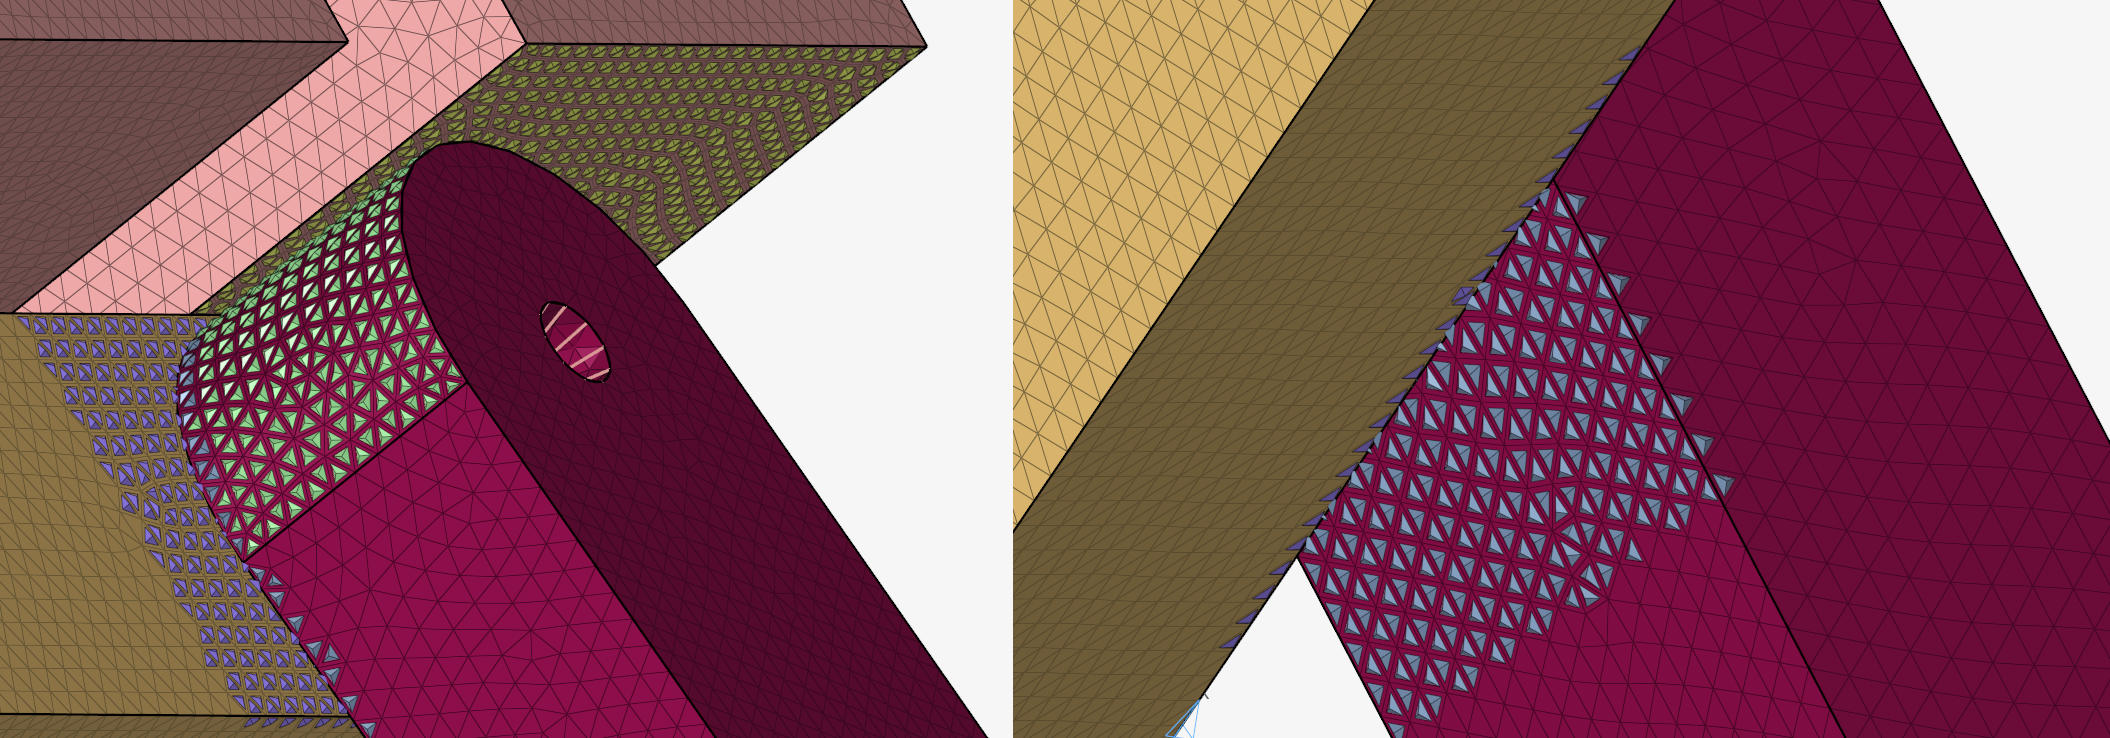
\includegraphics[height=4.5cm]{pics/09_Contact.png}
    \vspace{-0.4cm}
    \caption{\small{接触设置示意图}}
    \vspace{-0.4cm}
\end{figure}
\par{}
然而，图9中的Property Option设置为Property Type、TYPE设置为SLIDE（无摩擦滑动、只传递挤压）或STICK（粘连、有摩擦且传递拉压）时，仅适用于非线性静态（Non-linear Static）分析，线性分析时接触不生效；而FREEZE（完全粘结）虽然适合线性分析但不符合实际情况。
\par{}
实践证明非线性分析所耗时间较长（每种工况所需1小时以上）且不一定兼容后续分析，又注意到小变形问题加之RBE2约束使得接触不生效的情况与有接触的情况近似，为了提高效率，只能采用线性分析而暂时放弃已设置的接触。
\par{}
因此，接触种类设定为SLIDE，并预留非线性求解接口（此算例线性分析时不生效）；其他不进行改动，让求解器自行选择线性分析以节省求解时间。
\subsection{\heiti{静态特性分析条件设置}}
\par{}
静态分析的目的主要是求解结构在恒定、时不变载荷作用下的位移、应力和应变，适用于线性和非线性（大变形、材料非线性、接触）问题，是结构强度/刚度校核最常用的分析类型。
\subsubsection{\heiti{工况一：单人站立于顶板上}}
\par{}
假设一$\rm 80~kg$的人静立于顶板上，其鞋子宽度约$\rm 100~mm$，鞋长大约$\rm 270~mm$，略长于顶板总长（$\rm 240~mm$），因此可认为鞋子完全覆盖顶板长度；由于顶板中间存在间隙，按照图10所示的装配图计算得接触长度为$\rm 4 \times 45~mm =  180~mm$。因此双脚与顶板接触面积为$\rm 2 \times 100~mm \times 180~mm = 36000~mm^2$，不考虑重心位置，人对顶板的压强为$\rm 80~kg \times 9.8~N/kg \div 36000~mm^2 \approx 0.02178~MPa$，因此在顶板上设置一个面积为约$\rm 100~mm \times 180~mm$、压强为$\rm 0.02178~MPa$的均布载荷，点击“Analyze~→~Loads~→~Pressures”设置加载压强并单独分组。
\par{}
\begin{figure}[htbp]
    \centering
    \vspace{-0.1cm}
    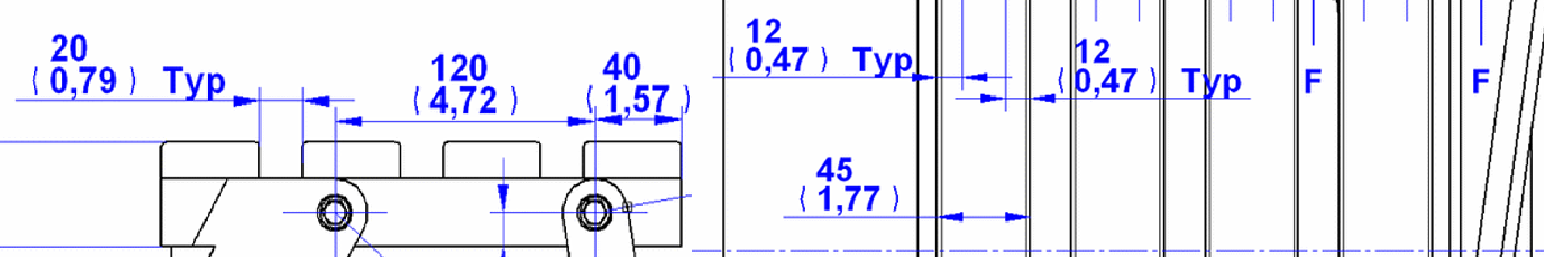
\includegraphics[width=\linewidth]{pics/10_TP.png}
    \vspace{-1cm}
    \caption{\small{装配图（局部）}}
    \vspace{-0.4cm}
\end{figure}
\subsubsection{\heiti{工况二：单人两脚分别站立于两个梯级上}}
\par{}
假设一$\rm 80~kg$的人一脚踏在第一级梯级、另一脚踏在第二级梯级上，其鞋子宽度约$\rm 100~mm$，鞋长大约$\rm 270~mm$，长于梯级宽度（如图11，$\rm 94~mm$），因此可认为鞋子完全覆盖梯级宽度。因此双脚与梯级接触面积为$\rm 2 \times 100~mm \times 94~mm = 18800~mm^2$，不考虑重心位置，人对梯级的压强为$\rm 80~kg \times 9.8~N/kg \div 18800~mm^2 \approx 0.04170~MPa$，因此在梯级上设置一个面积为约$\rm 100~mm \times 94~mm$、压强为$\rm 0.04170~MPa$的均布载荷，点击“Analyze~→~Loads~→~Pressures”设置加载压强并单独分组。
\par{}
\begin{figure}[htbp]
    \centering
    \vspace{-0.1cm}
    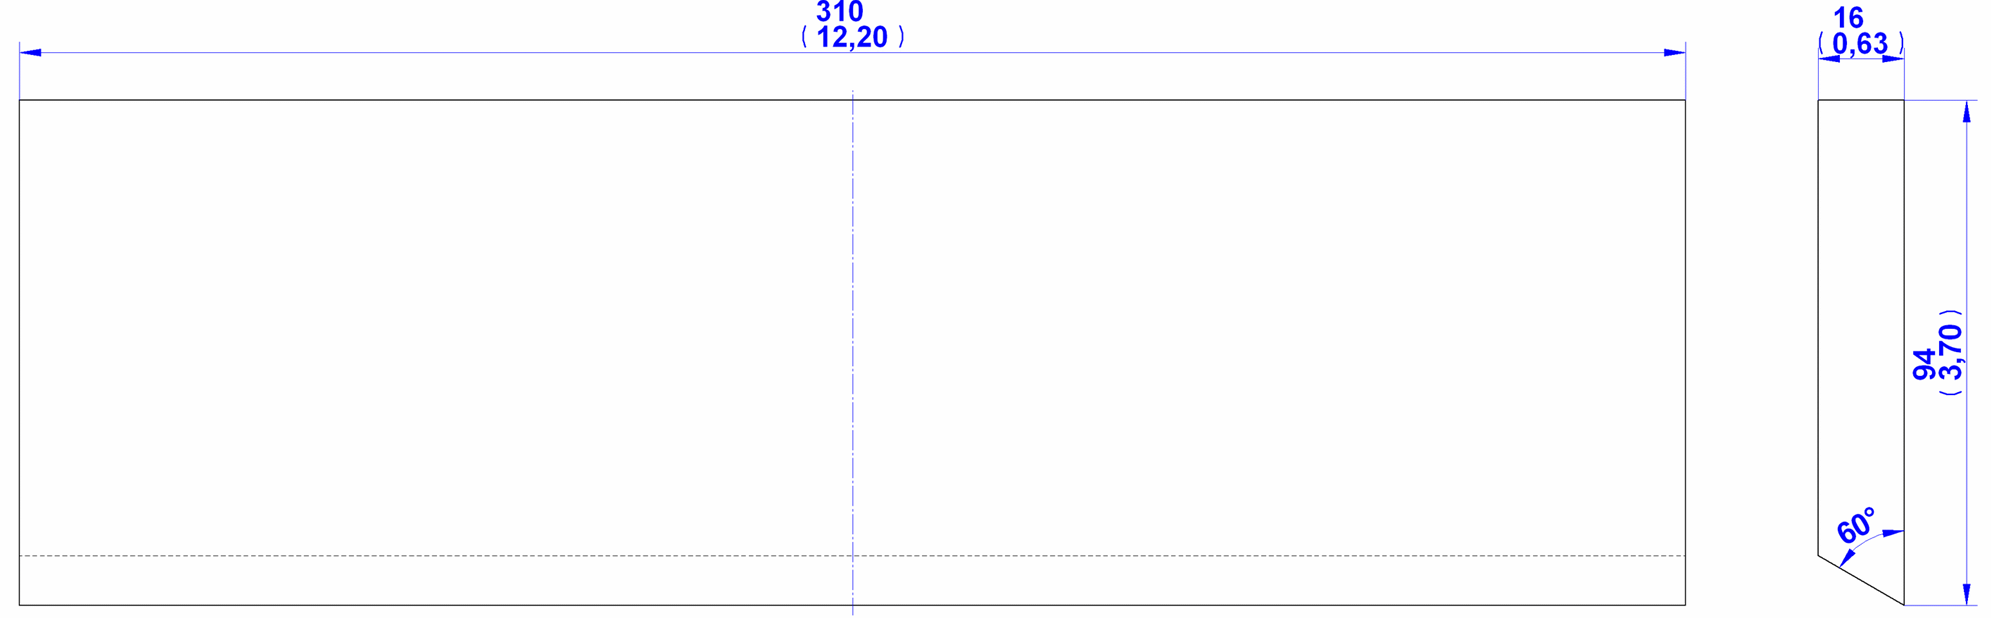
\includegraphics[width=\linewidth]{pics/11_Step.png}
    \vspace{-1cm}
    \caption{\small{装配图（局部）}}
    \vspace{-0.4cm}
\end{figure}
\subsubsection{\heiti{静态特性分析加载步设置}}
\par{}
两种工况载荷示意图如图12（粉色面上偏绿/偏蓝处）。点击新建两个加载步（Load Steps），设定分析种类（Analyze Type）为线性静态分析（Linear Static），并分别添加同一个约束与对应的载荷组。最终设置结果如图12。
\par{}
\begin{figure}[htbp]
    \centering
    \vspace{-0.1cm}
    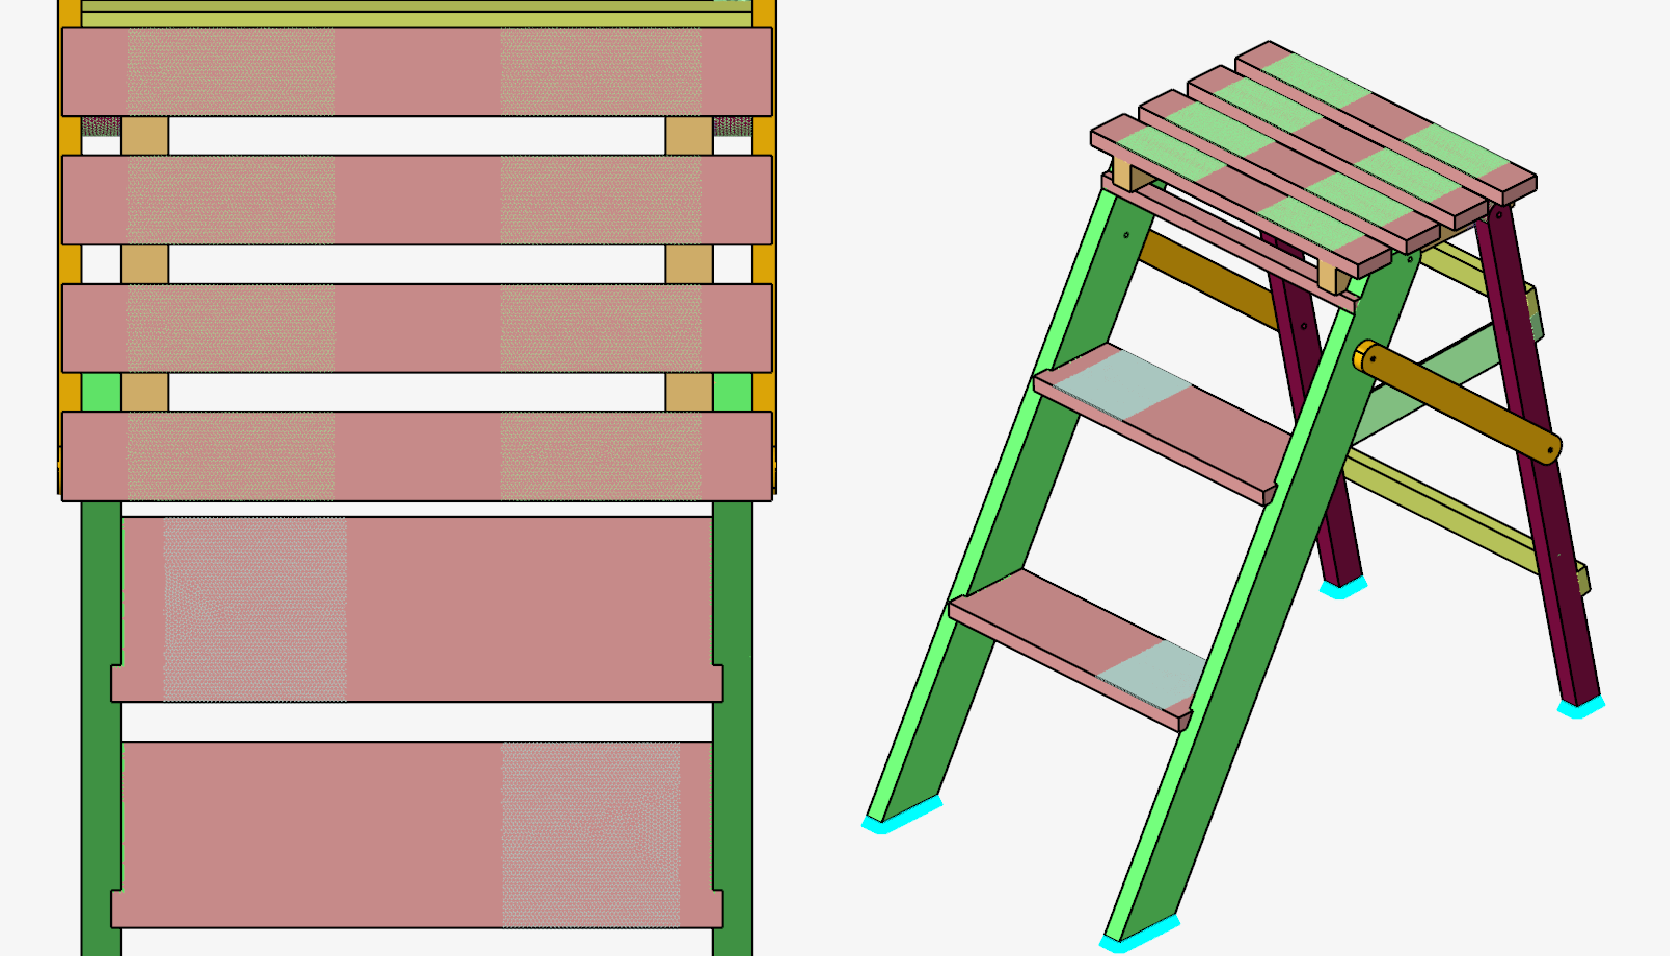
\includegraphics[height=5cm]{pics/12_Loads.png}
    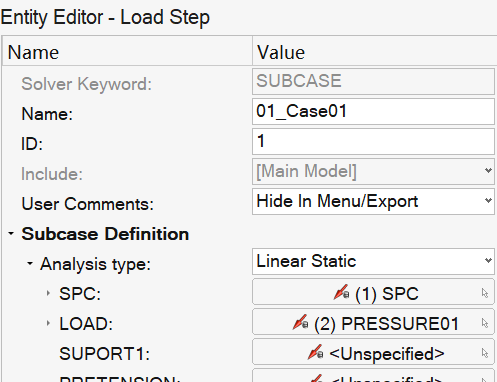
\includegraphics[height=4cm]{pics/12_Loadsteps.png}
    \vspace{-0.4cm}
    \caption{\small{负载与加载步示意图}}
    \vspace{-0.4cm}
\end{figure}
\subsection{\heiti{动态特性分析条件设置}}
\par{}
动态特性分析包括模态分析、频率响应分析、瞬态响应分析、随机振动分析等。
\par{}
其中，模态分析用于求解结构的固有频率和对应的振型，用于避开共振、评估结构刚度分布合理性，同时也是是频率响应分析、瞬态特性分析、随机振动分析（均为模态法时）的基础；
\par{}
频率响应分析目的是求解结构在正弦简谐周期载荷下的稳态响应，用于评估结构在不同频率激励下的动力学特性，输入为幅值和频率变化的周期载荷，输出为位移、速度、加速度、应力随频率的变化，分直接法（求解耦方程）和模态法（先解耦再叠加），识别共振峰值；
\par{}
瞬态响应分析目的是求解结构在任意时间变化载荷下的响应，可处理冲击、碰撞、脉冲等短历时载荷，用于模拟载荷突变等时间相关事件；
\par{}
随机振动分析用于求解结构在随机振动载荷下的统计响应，输入为功率谱密度（PSD）函数，描述载荷在频域的能量分布，基于频响分析结果，利用统计学方法计算响应，输出为位移、应力等的均方根（RMS）值和功率谱密度，结果具有概率统计意义，适用于车辆路面颠簸、航空器湍流、地震载荷等情境。
\subsubsection{\heiti{模态分析条件设置}}
\par{}
如果人只是站在折叠梯上进行手动维修等操作，频率一般为$\rm 200~Hz$以下。因此，主要对$\rm 0$~\textasciitilde~$\rm 200~Hz$范围内的频率进行分析。
\par{}
本算例针对较大模型，采用AMSES分析法（Autometic Multi-Level Sub-Structuring Eigensolver Solution，自动多层级子结构特征值求解，对应EIGRA）。这种分析法虽然没有兰索斯法（Lanczos，对应EIGRL）精确，但针对较大模型性能比Lanczos法优秀，且精度差距较小。
\par{}
先建立EIGRA，设置频率范围（V1、V2）为$\rm 0$~\textasciitilde~$\rm 200~Hz$，模态数上限（ND）空置，归一化选项（NORM）设置为质量归一化（MASS）。这样可以在指定频率中分析，限制频率范围以节省求解时间与存储空间。实践证明，计算时Optistruct程序会将内存中无法容纳的数据存储在外存（硬盘）中，仅$\rm 0$~\textasciitilde~$\rm 200~Hz$范围内就占用了约$\rm 30~GB$，如果不限制范围，只限制模态数，可能会导致硬盘空间耗尽。
\par{}
同时，虽然折叠梯使用还面临其他情景——如手持电钻的高频激励——但实践表明当求解$\rm 1990$~\textasciitilde~$\rm 2100~Hz$区间的仅仅1阶模态时，硬盘仍旧会空间耗尽而导致程序报错。猜测由于程序求解高频段的激励时仍然会从最低频率开始，因此仍然会向硬盘中存储较大内容。
\subsubsection{\heiti{模态分析加载步设置}}
\par{}
接下来针对此频率范围建立加载步，设定分析种类为正则振动模态（Normal Modes），并添加和上一小节同一个约束；结构方法（METHOD (STRUCT)）一栏设置为对应的EIGRA。最终设置结果如图13（包含$\rm 1990$~\textasciitilde~$\rm 2100~Hz$的情景，但该情景运算失败，因此没有纳入后续报告）。
\par{}
\begin{figure}[htbp]
    \centering
    \vspace{-0.1cm}
    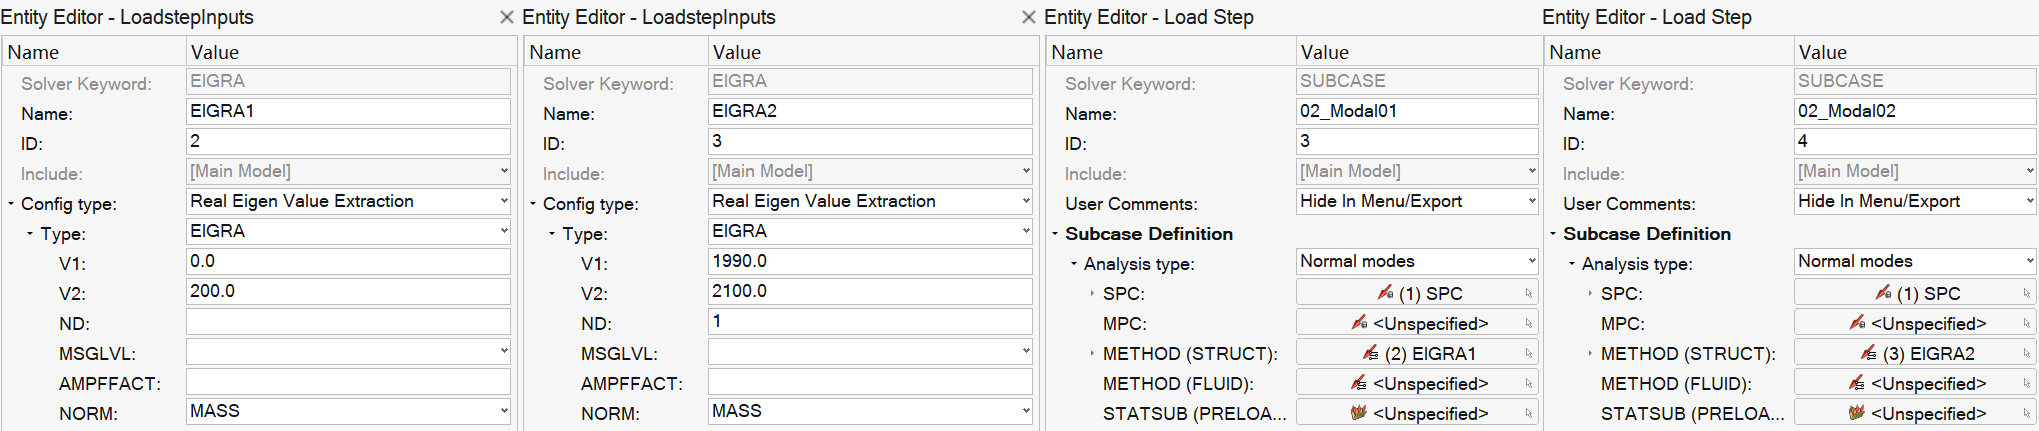
\includegraphics[width=\linewidth]{pics/13_Loadsteps.png}
    \vspace{-1cm}
    \caption{\small{模态范围与加载步示意图}}
    \vspace{-0.4cm}
\end{figure}
\subsubsection{\heiti{频率响应分析条件设置}}
\par{}
该步骤可以通过软件自带的模板（“Analyze~→~Templates~→~Unit~Input~Frequency~Response”）完成，也可以手动搭建。由于尝试使用模板时发现效果不理想，故改为手动搭建。同时这些步骤会增加较多的设定，不利于管理，因此需对该模型新建一个分支，再在分支内进行设置。
\par{}
首先复制一份模型文件，使用RBE3单元连接需要加周期振动载荷的区域，以方便直接添加单一载荷力并均布到这些区域。这里直接选用静态特性分析工况一的区域，并实行选择稀释，即隔几个节点选一个；当然也可以直接选取所有节点并直接划分到一个RBE3单元内，但这会在运算时抛出内存溢出错误，即使开启了外存转换（-core~OUT），推测是因为超大RBE3导致预处理阶段矩阵过大，从而还未等到计算开始、启动外存转换就已经崩溃。故应当稀释选择的节点，这里稀释到原来的约$1/3$，这样可以减少预处理阶段的矩阵大小，避免内存溢出。最终设置结果如图14。
\par{}
\begin{figure}[htbp]
    \centering
    \vspace{-0.1cm}
    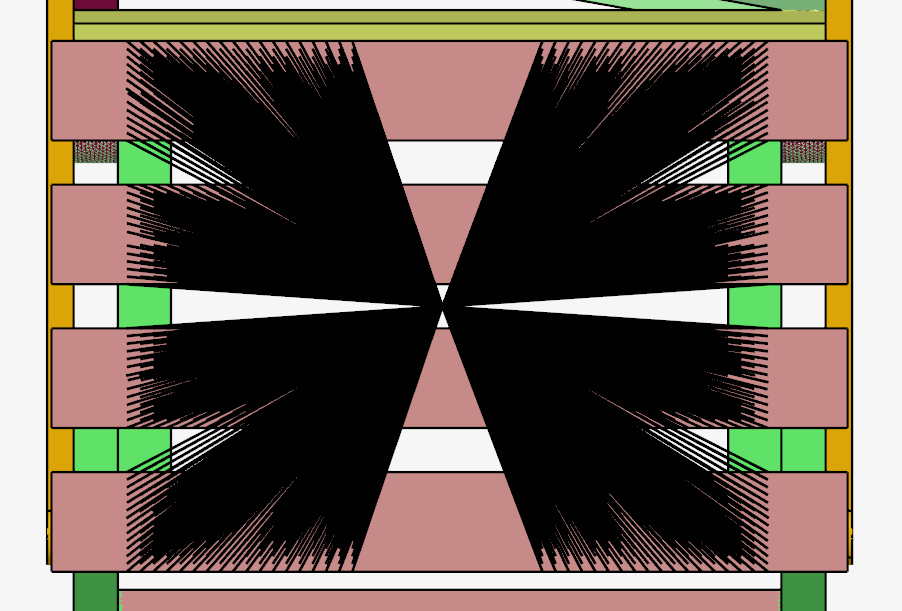
\includegraphics[height=4cm]{pics/14_RBE3.png}
    \vspace{-0.2cm}
    \caption{\small{RBE3划分示意图}}
    \vspace{-0.4cm}
\end{figure}
\par{}
对于频响分析，有直接法和模态法两种方法，直接法求解多频率问题效率低于模态法，更适合少量分析；这里为了模拟人在折叠梯顶端站立时的垂直振动，是小变形近似线性问题，可近似成垂直恒力与振动力叠加，位移也可近似看成是两个力单独作用时的位移的叠加。对于垂直恒力，我们已经在静态特性分析中的工况一中完成分析，因此这里只需要分析振动力单独作用的效果。因此新建动态载荷。我们分析的目标频率在人体自振频率范围附近，即1\textasciitilde20~Hz，步长为1~Hz，数量较少，可以选择直接法进行分析。故载荷应该加DAREA，作用点选择先前建立的RBE3单元的中心点（从动点），仅勾选DOF2（$y$轴平动方向），设置幅值为-10，模拟初始方向向下的、幅值为10~N的周期力。
\par{}
再新建频率范围。如上段所说，我们需要分析1\textasciitilde20~Hz，步长为1~Hz的频率段，故新建FREQi，在其中勾选FREQ1，初始频率（F1）选择1，步长（DF）选择1，频率数量（NDF）选择19即可。
\par{}
同时还要先确定最终展示的点集，右键创建“SET\_GRID”，依次选择目标节点，这里选择了每个部件的中心点，共16个点，这16个点的位置见分析结果；其他设置保持默认。
\par{}
然后新建一个TABLED1表格以存放频率，新建后右键单击选择”参考”（References），在参考列表中再次右键单击选择”编辑”（Edit），输入以下数据：
\begin{equation*}
    \begin{bmatrix}
          & X    & Y   \\
        1 & 0.0  & 1.0 \\
        2 & 50.0 & 1.0
    \end{bmatrix}
\end{equation*}
其他保持默认即可。
\par{}
再添加RLOAD2。类型（Config Type）选择动态载荷-基于频率（Dynamic Load - Frequency Dependent），激励ID（Exciteid）选择先前建立的DAREA，TB和TP选择先前建立的TABLED1，TP类型选择载荷（LOAD）。
\par{}
最后添加系统阻尼。在新建窗口中选择“参数”（PARAMS）卡片，点击设置其为激活状态，勾选G并设置为0.06即可。还可以勾选耦合质量矩阵求解（COUPMASS - YES）。
\subsubsection{\heiti{频率响应分析加载步设置}}
\par{}
新建加载步，分析类型选择直接法频响分析（Freq. resp (direct)），SPC、DLOAD和FREQ分别选择先前设定的SPC、DAREA、FREQi；下方的工况选项（Subcase Options）勾选OUTPUT及其子目录下的ACCELERATION、DISPLACEMENT、VELOCITY，即加速度、位移和速度，格式（FORMAT）均选择H3D，选项（OPTION）选择SID，SID选择先前建立的点集即可。最后新建全局输出请求（GLOBAL\_OUTPUT\_REQUEST）卡片在里面作和加载步相同的设置。
\subsubsection{\heiti{瞬态响应分析条件设置}}
\par{}
同\textbf{5.3.3.}，先复制一份文件、建立新的分支，再在分支内进行设置。和频响分析不同，瞬态响应分析主要通过时域响应来观察物体状态变化，因此更加直观，还可以通过输出动画来查看结果。
\par{}
本次要模拟的是人从地面上走上扶梯的过程。该过程可分解为：人站在地面上，右脚先踏上第一级梯级，其后全身重量都作用在该级梯级上并保持稳定。因此需要对该情境设定力的变化曲线以符合真实情况。
\par{}
首先清理工况二中所加载在梯级上的PLOAD4载荷。将第二级梯级上的压力清理掉，只保留第一级的。接着添加TABLED1以存放力的时域图像。同样地，在TABLED1中输入如下数据：
\vspace{0.2cm}
\par{}
\begin{minipage}{0.48\textwidth}
    \begin{equation*}
        \begin{bmatrix}
               & X    & Y        \\
            1  & 0.0  & 0.0      \\
            2  & 0.02 & 1.020108 \\
            3  & 0.05 & 4.591836 \\
            4  & 0.07 & 3.82653  \\
            5  & 0.08 & 3.061224 \\
            6  & 0.09 & 2.55102  \\
            7  & 0.1  & 2.295918 \\
            8  & 0.15 & 2.040816 \\
            9  & 0.2  & 2.015306 \\
            10 & 0.3  & 2.0      \\
            11 & 0.5  & 2.0      \\
            12 & 5.0  & 2.0
        \end{bmatrix}
    \end{equation*}
\end{minipage}
\begin{minipage}{0.48\textwidth}
    \centering
    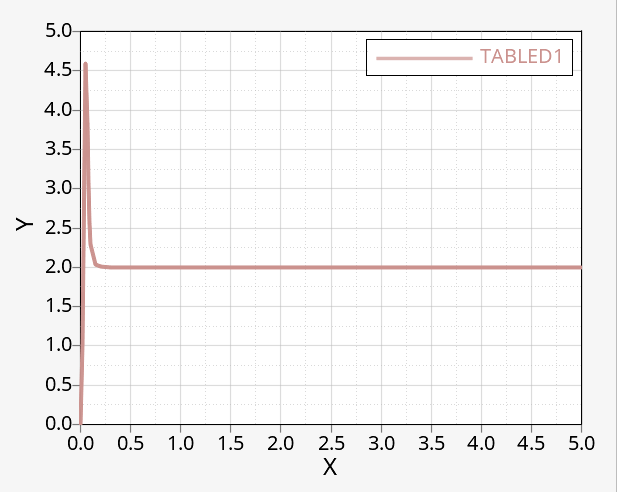
\includegraphics[width=\linewidth]{pics/15_Figure.png}
    \vspace{-0.2cm}
    \captionof{figure}{\small{力的倍数图像示意图}}
\end{minipage}
\vspace{0.2cm}
\par{}
图15是加载力的倍数图像，由于模拟的情况是人单脚站上梯级，故以2倍为稳定值；而刚踏上梯级时，梯级受力可达到稳定值的两倍多，后再趋于稳定。因此经计算后TABLED1如上设置。
\par{}
接着创建TLOAD1载荷，激励ID选择已修改的工况二PLOAD4，时间ID（TID）选择先前创建的TABLED1，类型选择LOAD即可。当然也可以创建TLOAD2，但比前者复杂，故仍选择TLOAD1。
\par{}
最后创建TSTEP卡片，数量（N）和步长（DT）设置为0.01与500，即5~s。需要注意的是，正常情况下人是不会单脚站立在梯级上约5~s的，这样做只是为了查看梯级的振动情况，实际上该状态可能最多持续1~s。
\subsubsection{\heiti{瞬态响应分析加载步设置}}
\par{}
新建加载步，分析类型选择直接法瞬态分析（Transient (direct)），SPC、DLOAD和TSTEP分别选择先前设定的SPC、TLOAD1、TSTEP；下方的工况选项勾选OUTPUT及其子目录下的DISPLACEMENT、STRESS，即加速度与应力，格式均选择H3D，选项选择ALL。最后新建全局输出请求卡片在里面作和加载步相同的设置。
\par{}
最后添加系统阻尼，同\textbf{5.3.4}，设置G为0.6。
\subsubsection{\heiti{随机振动分析条件设置}}
\par{}
同\textbf{5.3.3.}，先复制一份文件、建立新的分支，再在分支内进行设置。和前几种分析的目的不同，随机振动分析主要通过对输入的功率密度谱（输入能量在频率上的分布，即PSD）的位移或应力等响应求均方根值（电学中称有效值，即RMS），来判断在一定范围内的、已知能量统计规律的不确定频率的激励下，结构是否满足应力等要求。
\par{}
本次要模拟的是0\textasciitilde20~Hz内的随机地面振动对静置无载荷折叠梯的影响。
\par{}
首先设置加速度激励SPCD。该激励一般是基于SPC约束建立的，由于主分支中已经设定了约束，故直接在该约束所在的点位上建立SPCD，设置dof2，即$y$轴分量为1，其他为0。
\par{}
建立TABLED1曲线，输入如下数据确定频率范围：
\begin{equation*}
    \begin{bmatrix}
          & X  & Y \\
        1 & 0  & 1 \\
        2 & 20 & 1
    \end{bmatrix}
\end{equation*}
然后直接创建RLOAD2，激励ID选择先前创建的SPCD，TB选择先前建立的TABLED1，TP空置，类型选择加速度（ACCE），其他设置同\textbf{5.3.3.}即可。
\par{}
由于随机振动分析是基于频率响应分析完成的，而由于之前已经使用过直接法，我们本次练习使用模态法进行频率响应分析，因此仍需要先新建EIGRL/EIGRA，这里选择后者，只设定N2为20即可。
\par{}
接着设定阻尼曲线。新建TABDMP1表格，输入阻尼数据：
\begin{equation*}
    \begin{bmatrix}
          & X  & Y    \\
        1 & 0  & 0.06 \\
        2 & 20 & 0.06
    \end{bmatrix}
\end{equation*}
\par{}
再新建FREQi卡片，可以勾选FREQ1或FREQ3，FREQ3基于扫频的频率的间隔，增加分析频率的数量，会增加计算负担，这里由于性能有限，同时因为先前做的模态分析中，0\textasciitilde20~Hz的模态较为密集且可近似视为均匀分布，选择FREQ1，设定F1、DF、NDF分别为0.5、0.5、39，即从0.5到20、步长0.5、个数39即可，注意D1不可设置为0，否则后续分析会报错。
\par{}
接着再新建TABRND表格，输入功率谱密度（PSD）函数，这里输入：
\vspace{0.5cm}
\par{}
\begin{minipage}{0.48\textwidth}
    \begin{equation*}
        \begin{bmatrix}
              & X  & Y    \\
            1 & 0  & 0    \\
            2 & 1  & 50   \\
            3 & 4  & 5000 \\
            4 & 16 & 5000 \\
            5 & 20 & 4200 \\
        \end{bmatrix}
    \end{equation*}
\end{minipage}
\begin{minipage}{0.48\textwidth}
    \centering
    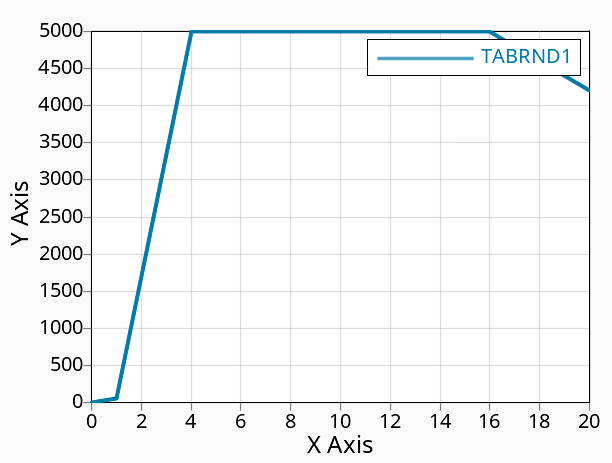
\includegraphics[width=\linewidth]{pics/16_Figure.png}
    \vspace{-1cm}
    \captionof{figure}{\small{功率谱密度函数图像示意图}}
\end{minipage}
\vspace{0.2cm}
\par{}
注意这里单位是$\rm {mm^2}/{s^5}$，因此要在原$\rm {g^2}/{Hz}$的基础上乘以$9800^2$，最终图像如图16。对该图像进行积分得：
\[
    \begin{aligned}
        A_1 & \;(0\text{\textasciitilde}1\;\text{Hz}):   & \frac{0 + 50}{2} \times (1-0)        & = 25                          \\
        A_2 & \;(1\text{\textasciitilde}4\;\text{Hz}):   & \frac{50 + 5000}{2} \times (4-1)     & = 7,575                       \\
        A_3 & \;(4\text{\textasciitilde}16\;\text{Hz}):  & 5000 \times (16-4)                   & = 60,000                      \\
        A_4 & \;(16\text{\textasciitilde}20\;\text{Hz}): & \frac{5000 + 4200}{2} \times (20-16) & = 18,400                      \\
        A   &                                            &                                      & = 86,000 \; (\text{mm/s}^2)^2
    \end{aligned}
\]
\begin{equation*}
    RMS = \sqrt{86,000} \approx 293.3 \; \text{mm/s}^2\approx 0.03g
\end{equation*}
即加速度有效值约为0.03倍重力加速度，大致符合日常使用场景。
\par{}
最后新建RANDPS，J和K都设置为先前建立的FREQi，X和Y（实部和虚部）分别设置为1.0和0.0，TID设置为TABRND即可。
\subsubsection{\heiti{随机振动分析加载步设置}}
\par{}
首先新建前置频响分析加载步，分析类型选择模态法频响分析（Freq. resp (modal)），SPC选择初始创建的SPC，DLOAD选择本次创建的RLOAD2，方法（结构）（METHOD (STRUCT)）选择本次创建的EIGRA，FREQ选择本次创建的FREQi即可，阻尼（结构）（SDAMPING (STRUCT)）选择本次创建的TABDMP1表格即可。
\par{}
再创建随机振动分析步本身，分析类型选择随机（Random），下方的大写RANDOM选择RANDPS，勾选输出并选择加速度、位移、应力，其他设置同\textbf{5.3.6.}即可。
\subsection{\heiti{稳定性分析条件设置}}
\par{}
稳定性分析目的是确定结构在受压载荷下发生失稳（屈曲）的临界载荷和屈曲模态，用于细长杆、薄壁结构、受压板件等易失稳构件的校核。
\subsubsection{\heiti{确定线性屈曲失稳临界载荷因子范围}}
\par{}
已知有限元分析中，失稳临界载荷有如下公式：
\begin{equation*}
    P_{\rm cr} = BLF \cdot P_i
\end{equation*}
其中，$P_{\rm cr}$为失稳临界载荷，$BLF$为失稳临界载荷因子（Buckling Load Factor），$P_i$为某工况静态特性分析时所施加的载荷。
\par{}
有限元仿真中，一般求解器会在给定的求解范围内给出多个$BLF$，以及每个$BLF$对应的失稳模态下的失稳应变云图。HyperMesh中，需要通过手动配置求解范围来限制$BLF$的范围或数量。
\par{}
在\textbf{5.2.1.}与\textbf{5.2.2.}中，我们详细解释了两种工况的载荷设置，因此，以这两种工况为基础进行分析。其中，我们模拟的是$\rm 80~kg$的人站立于折叠梯的某些区域上，根据接触面积估算出了仿真时所需要施加的压强。因此，折叠梯的日常使用工况应在5倍正常人体重以下，超出该范围可认为失稳模态不影响正常使用。
\par{}
但即使不影响正常使用，为了留出一定裕度并观察失稳模态特征，仍然设立较宽的$BLF$范围，如在0~\textasciitilde~100之间。
\subsubsection{\heiti{稳定性分析加载步设置}}
\par{}
由于软件进行失稳分析时仅支持兰索斯法，因此新建EIGRL，直接把下限（V1）与上限（V2）按照$BLF$范围设置为0和100即可，模态数上限（ND）空置即可。
\par{}
\begin{figure}[htbp]
    \centering
    \vspace{-0.1cm}
    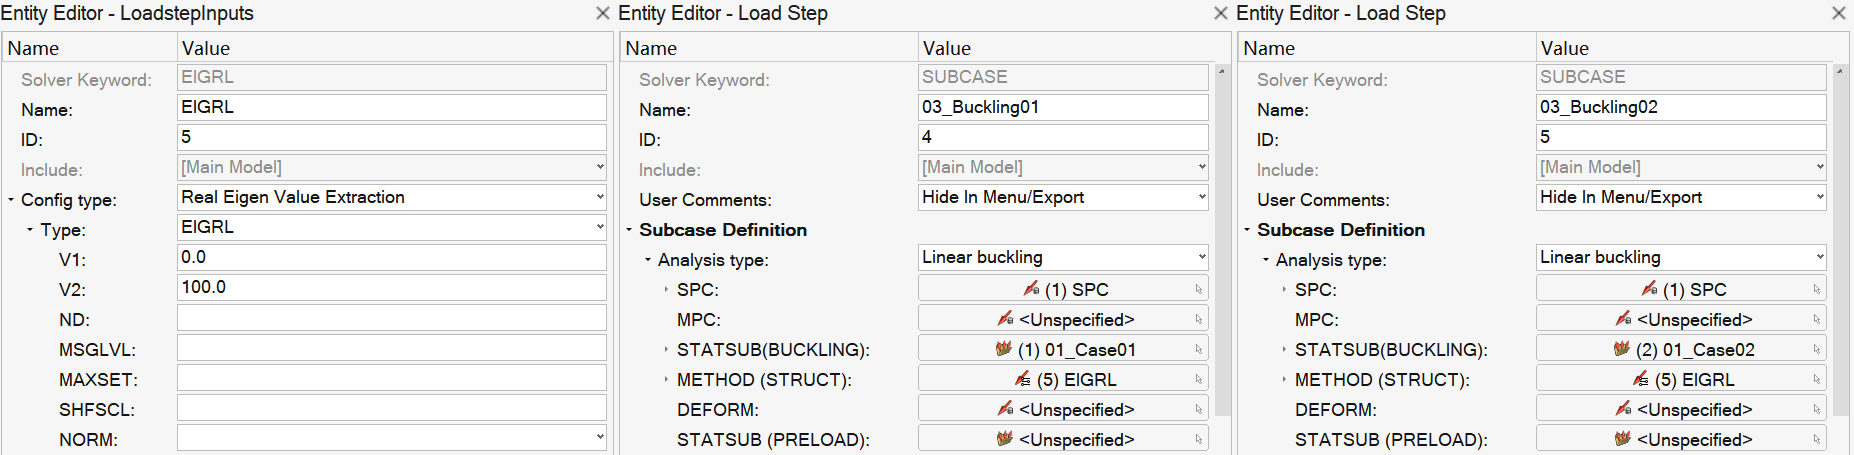
\includegraphics[width=0.75\linewidth]{pics/14_Loadsteps.png}
    \vspace{-0.3cm}
    \caption{\small{$BLF$范围与加载步示意图}}
    \vspace{-0.4cm}
\end{figure}
\par{}
再新建两个加载步，设定分析种类为线性屈曲（Linear Buckling），并添加与先前相同的约束，再将稳定性分析的工况（STATSUB~(BUCKLING)）分别设置为\textbf{5.2.1.}与\textbf{5.2.2.}的两个工况，再将同一个EIGRL添加至“方法”（METHOD~(STRUCT)）栏即可，如图17。
\subsection{\heiti{结构优化分析条件设置}}
\par{}
结构优化分析包括形貌优化分析、尺寸优化分析、形状优化分析与拓扑优化分析等。
\par{}
其中，形貌分析通常在薄壁结构上优化加强筋、压痕等凹凸形貌的分布，以提高刚度或改善模态，不改变材料厚度，仅改变表面几何形貌，常用于薄板壳体结构；
\par{}
尺寸优化分析可以优化结构的截面尺寸、板厚、材料参数等连续或离散变量，不改变拓扑和形状，只调整粗细、厚薄；
\par{}
形状优化分析主要在不改变拓扑的前提下，优化已有结构的边界或曲面形状以降低应力集中、改善疲劳寿命；
\par{}
拓扑优化分析主要在给定的设计空间内，寻找材料的最优分布，以最小化质量或最大化刚度，主要输出概念性形状，需要进行平滑处理等，同时也要尽量适应生产加工条件限制。
\subsubsection{\heiti{确定优化范围}}
\par{}
由于此算例为实体形态，因此选择”Optimize~→~Topology”进行拓扑优化。单击”Topology”按钮可以直接建立一个设计变量（Design Variables），其中属性类型（Property Type）一栏选择PSOLID，接着选择结构较为大块、远离受力复杂区域的范围，通过“Assembly~→~Organize”将其分配至新建部件并赋予属性（一般派生/复制自其原所在部件的属性），再进行拓扑优化。这里我们选择了折叠梯后支撑中部区域进行优化，如图18。
\par{}
为避免棋盘格等现象，应设定设计变量最小尺寸（Mindim）为2到3倍的网格尺寸，这里设为6；最大尺寸（Maxdim）应大于等于2倍的最小尺寸，这里选择12；最小间隔（Minimum Gap）默认等于最大尺寸，实际设置时也强制要求大于等于最大尺寸，这里也选择12。还可以设置拔模（Draw）或挤出（Extrusion）约束，以限制截面形状，或方便开模，这里由于是木材，不需要开模，又希望两侧后支撑形状相同，于是选择挤出约束，设置为“无扭转”（No twist）并选择$x$轴方向（垂直于前支撑侧面）为挤出路径。
\subsubsection{\heiti{确定优化响应、约束与目标}}
\par{}
接下来确定优化响应（Optimization Responses）。点击“Optimize~→~Responses”建立响应，我们进行优化的目的主要是在轻量化至一定范围内，同时应变不危险的情况下，让后支撑的刚度最大、柔度最小，因此分别将响应类型（Response Type）设置为静态位移（Static Displacement）、柔度（Compliance）和体积分数（Volumefrac），当然也可以选择其他的，如静态应力（Static Stress）、质量（Mass）等，设置如图18。其中，静态位移的节点选择顶板最上层的节点，柔度与体积分数分别选择后支撑剩余部分以及优化部分的体积分数。
\par{}
再确定优化约束（Optimization Constraints）。点击“Optimize~→~Constraints”建立约束，选择响应中的位移和体积分数进行约束，由于计算机资源有限，只选择工况1作为条件（即List of Loadsteps）；同时根据工况一的分析结果，设定位移上限为3~mm；根据轻量化目标，设定优化部分最终体积分数在0.5以下。
\par{}
还要确定优化目标（Objectives）。点击“Optimize~→~Objectives”建立目标，选择最小柔度作为目标，其他设置同前。
\subsubsection{\heiti{结构优化分析加载步设置}}
\par{}
由于上一小节已设置好静力学分析的工况一为前置加载步，此分析不需要设置任何加载步，只需点击“Optimize~→~Optimize”即可直接导出.fem文件进行分析。
\par{}
\begin{figure}[htbp]
    \centering
    \vspace{-0.1cm}
    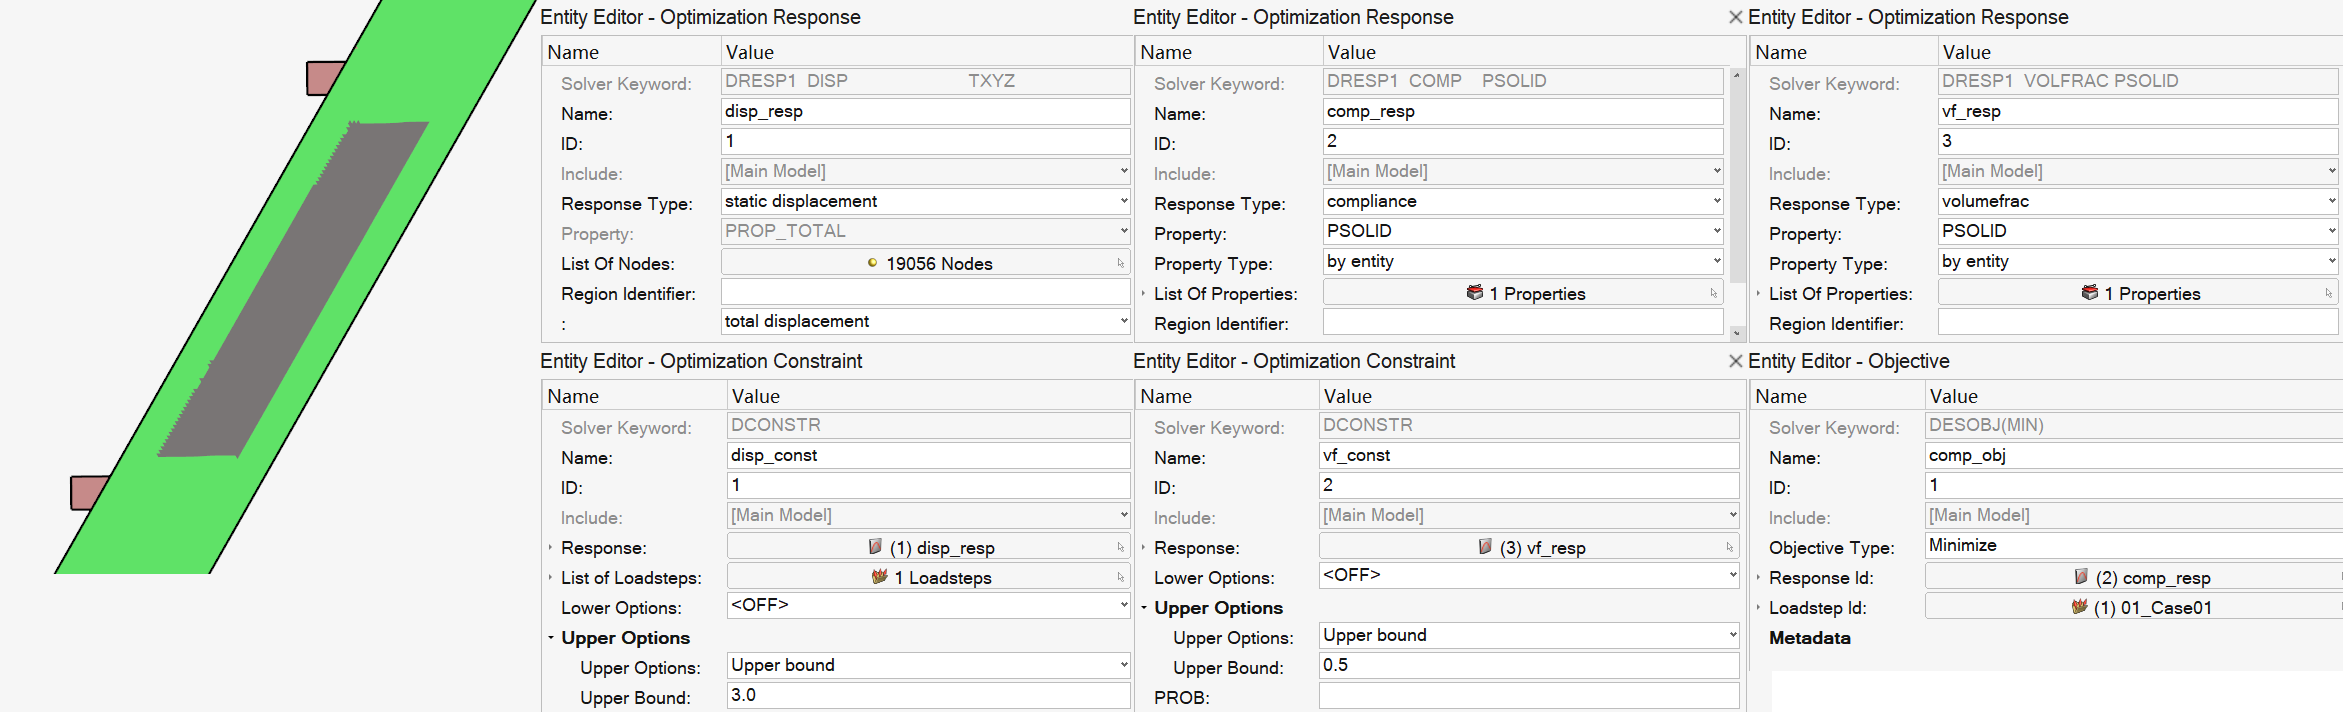
\includegraphics[width=0.98\linewidth]{pics/15_Loadsteps.png}
    \vspace{-0.3cm}
    \caption{\small{拓扑分析设置示意图}}
    \vspace{-0.4cm}
\end{figure}
\subsection{\heiti{疲劳分析条件设置}}
\par{}
疲劳分析的目的主要是评估结构在循环载荷反复作用下萌生裂纹并扩展直至破坏的寿命，用于周期性载荷构件的耐久性评估。
\subsubsection{\heiti{疲劳分析前置条件设置}}
\par{}
首先复制一份文件以新建新的分支。将静态特性分析中的工况二再拆分成两个工况，分别只包含单个梯级上的作用力（就是把工况二的两个梯级受力分开分析），原因见下文。同时还要将三个工况的OUTPUT勾选，其中还要勾选DISPLACEMENT和STRESS，格式均选择H3D、选项选择ALL，STRESS的类型（TYPE）也选择ALL，位置（LOCATION）选择CORNER，接着再在GLOBAL\_OUTPUT\_REQUEST卡片中做同样设置，原因同样见下文。和前几节同理，输出.fem文件并进行运算，得.h3d结果备用。
\subsubsection{\heiti{S-N曲线配置}}
\par{}
接着打开Altair HyperLife 2026，这是配套软件中专门用于疲劳寿命分析的软件。点击“File~→~Open File\dots~→~Open Model and Result Files”，在弹出的窗口中直接选择先前分析得到的.h3d文件。
\par{}
打开后点击“HyperLife~→~SN”选择S-N曲线进行寿命分析，并按图19进行设置。其中，木材是脆性各向异性材料，不存在屈服平台，适合高周疲劳分析，因此只能选择S-N曲线；方法（Method）只能选择多轴（Multi Axial），因为该算例模型十分复杂；单位（FE Model Units）直接选用默认的MPa即可；平面数（Number of Planes）设为36，这里的平面是指疲劳裂纹沿某个特定平面萌生，程序会在空间中按一定角度步长扫描所有可能的平面，找出损伤最大的那个，这里所有可能的平面的数量就是36，它们的角度间隔为5°，基本足够精确；幸存概率（Certainty of Survival）设为0.95，指设计寿命下不发生疲劳破坏的概率达到0.95；拉伸损伤模型（Tension Damage Model）选择古德曼（GOODMAN），这样较为简洁；剪切损伤模型（Shear Damage Model）选NONE，因为另一种，即FINDLEY是基于金属晶体位错滑移的，不适用于木材；层选择（Layer Selection）选择Worst，意为遍历实体单元的所有可用位置取损伤较大者；应力梯度修正（Stress Gradient）选择OFF，因为另一个是FKM相关，不适用于GOODMAN模型；载荷类型（Type of Loading）选择时间序列（Time Series），这可以按时间调整每次加载每一种载荷的作用。
\par{}
\begin{figure}[htbp]
    \centering
    \vspace{-0.1cm}
    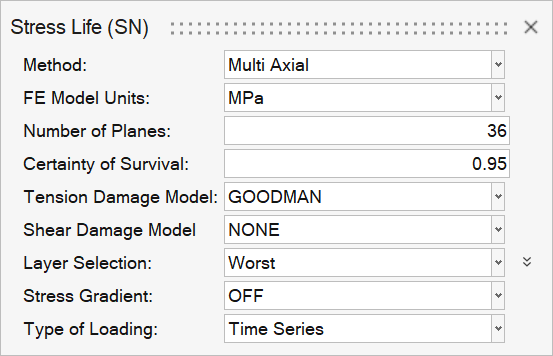
\includegraphics[height=4cm]{pics/19_SN.png}
    \vspace{-0.3cm}
    \caption{\small{S-N曲线初步设置示意图}}
    \vspace{-0.4cm}
\end{figure}
\begin{figure}[htbp]
    \centering
    \vspace{-0.1cm}
    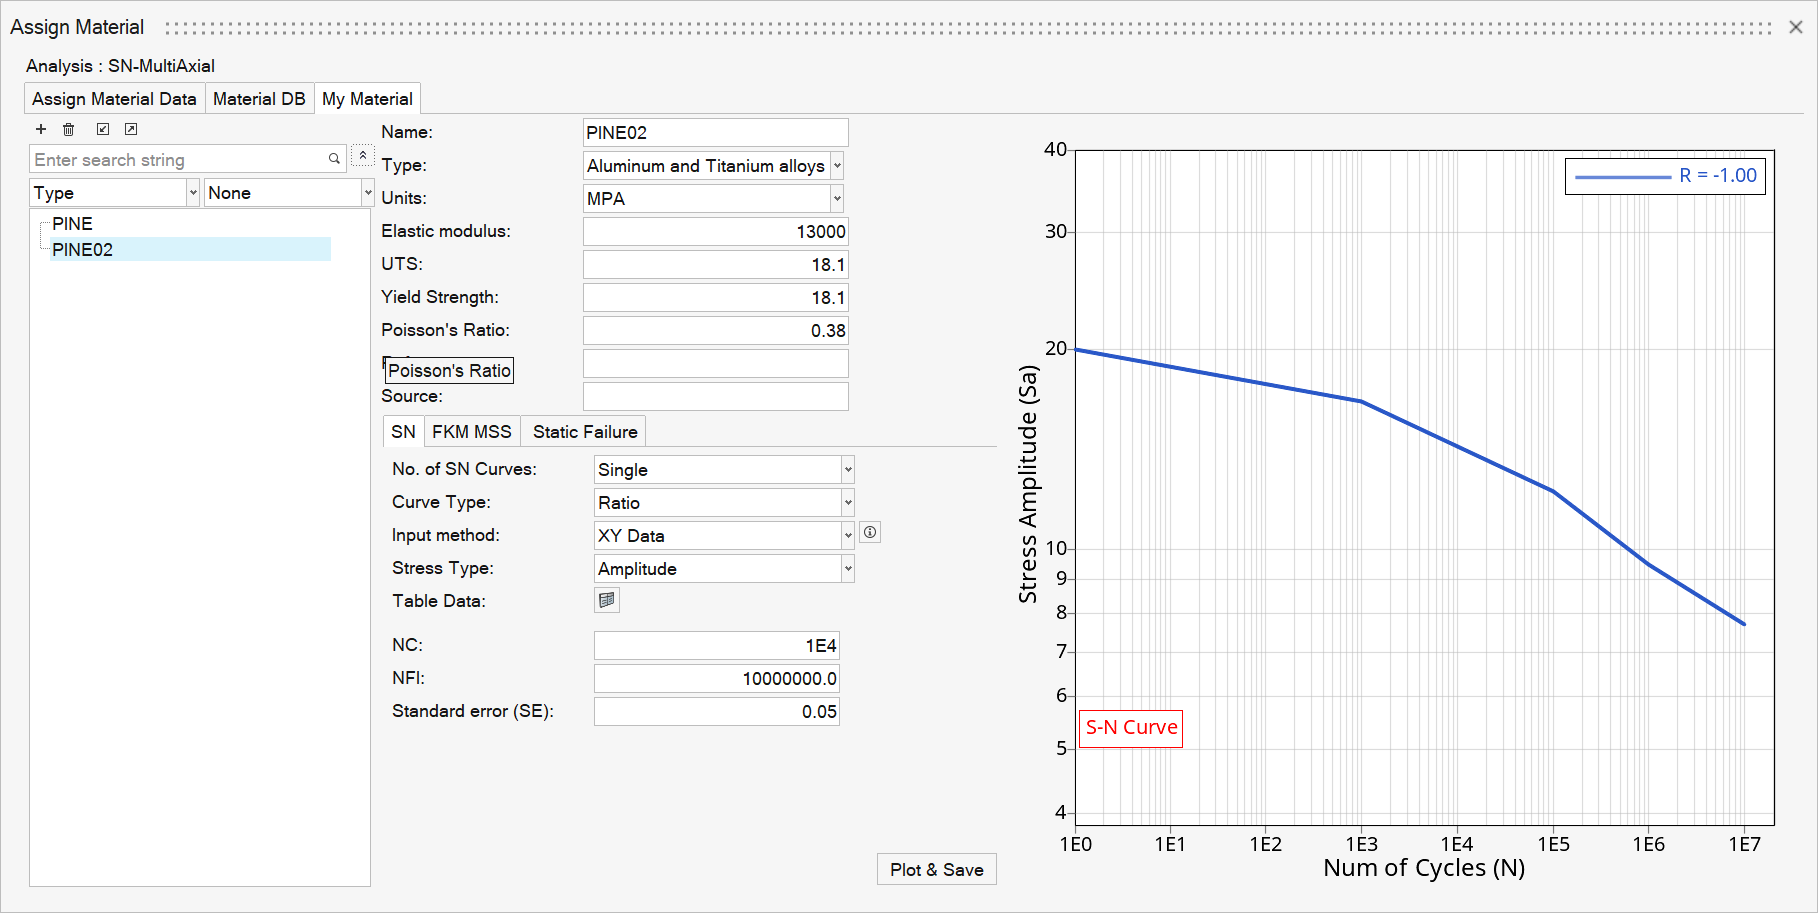
\includegraphics[width=0.98\linewidth]{pics/20_MAT.png}
    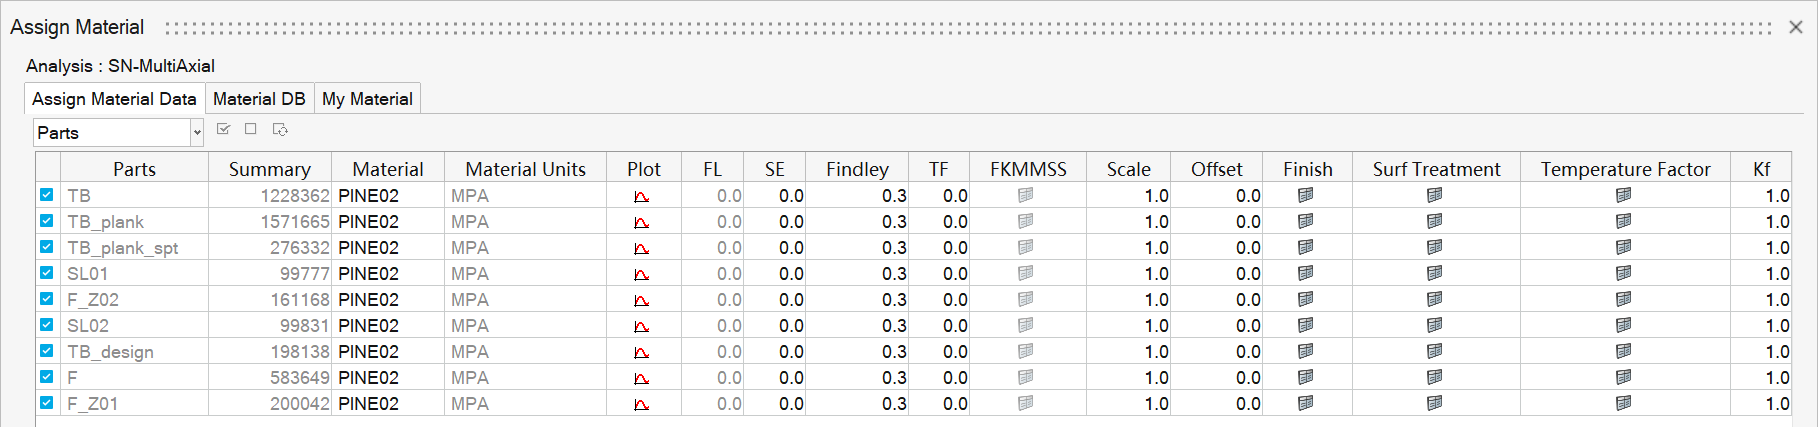
\includegraphics[width=0.98\linewidth]{pics/20_MAT2.png}
    \vspace{-0.3cm}
    \caption{\small{S-N曲线详细数值设置示意图}}
    \vspace{-0.4cm}
\end{figure}
\par{}
再点击“HyperLife~→~Material Setup”进行材料设置。在窗口中选择“我的材料”（My Material），单击加号新建材料，根据文献\textsuperscript{\textcolor{red}{\cite{ref2}}}中的数据设定各项指标如图20，需要注意的是，类型（Type）一栏只有钢、铝等金属材料，无法自定义，因此保持默认即可。
\par{}
其中，图线数据为：
\begin{equation*}
    \begin{bmatrix}
          & S    & N         \\
        1 & 20.0 & 1{\rm E}0 \\
        2 & 16.7 & 1{\rm E}3 \\
        3 & 14.3 & 1{\rm E}4 \\
        4 & 12.2 & 1{\rm E}5 \\
        5 & 9.5  & 1{\rm E}6 \\
        6 & 7.7  & 1{\rm E}7 \\
    \end{bmatrix}
\end{equation*}
\par{}
右击自定义的材料名称，点击“添加到材料指定列表”（Add to Material Assign List），再在“指定材料数据”（Assign Material Data）中勾选所有部件，并统一指定材料为先前创建的材料。此外还可以设定材料表面参数，单击“完成”（Finish）一列的小图标，选择“用户”（USER）并设定表面粗糙度为0.5即可。
\par{}
\begin{figure}[htbp]
    \centering
    \vspace{-0.1cm}
    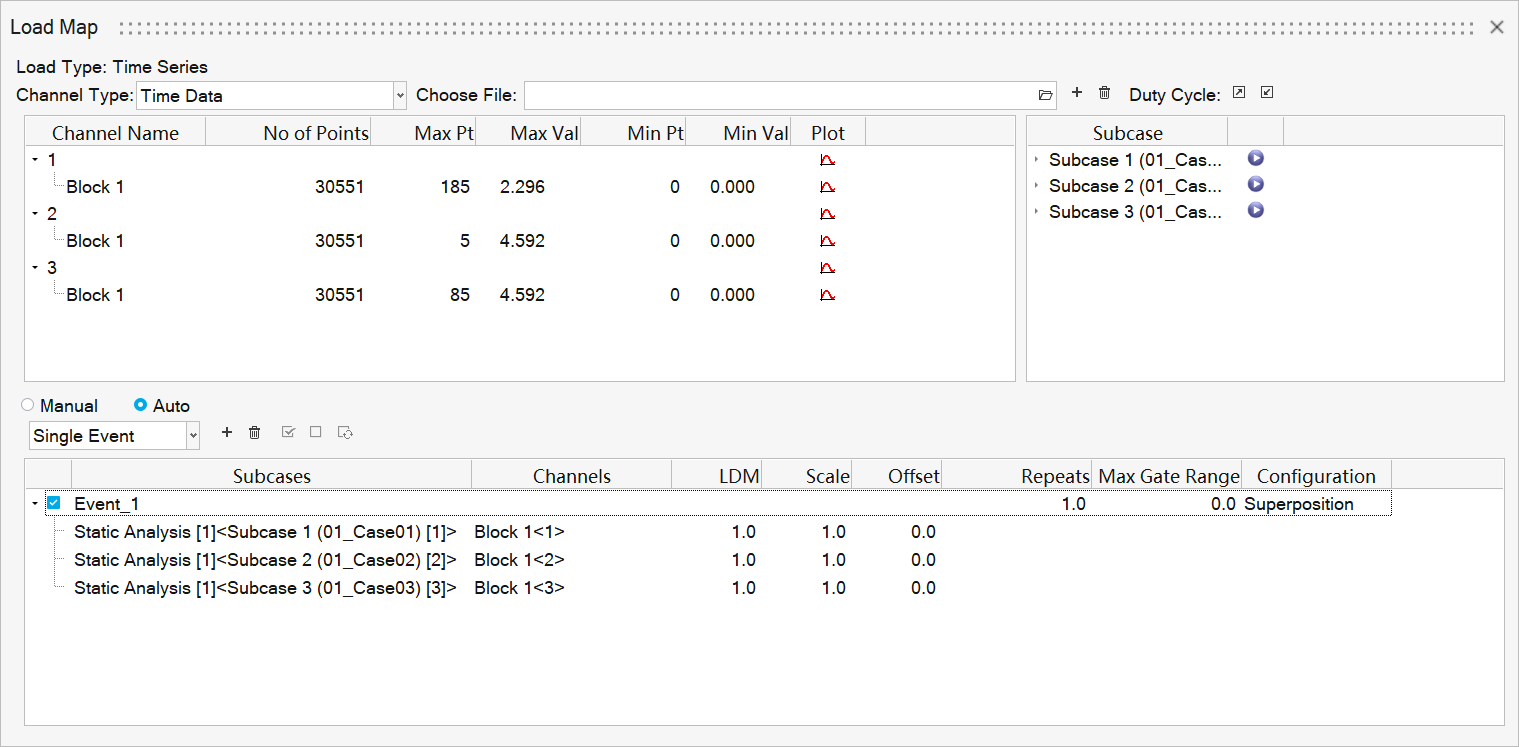
\includegraphics[width=0.98\linewidth]{pics/21_Event.png}
    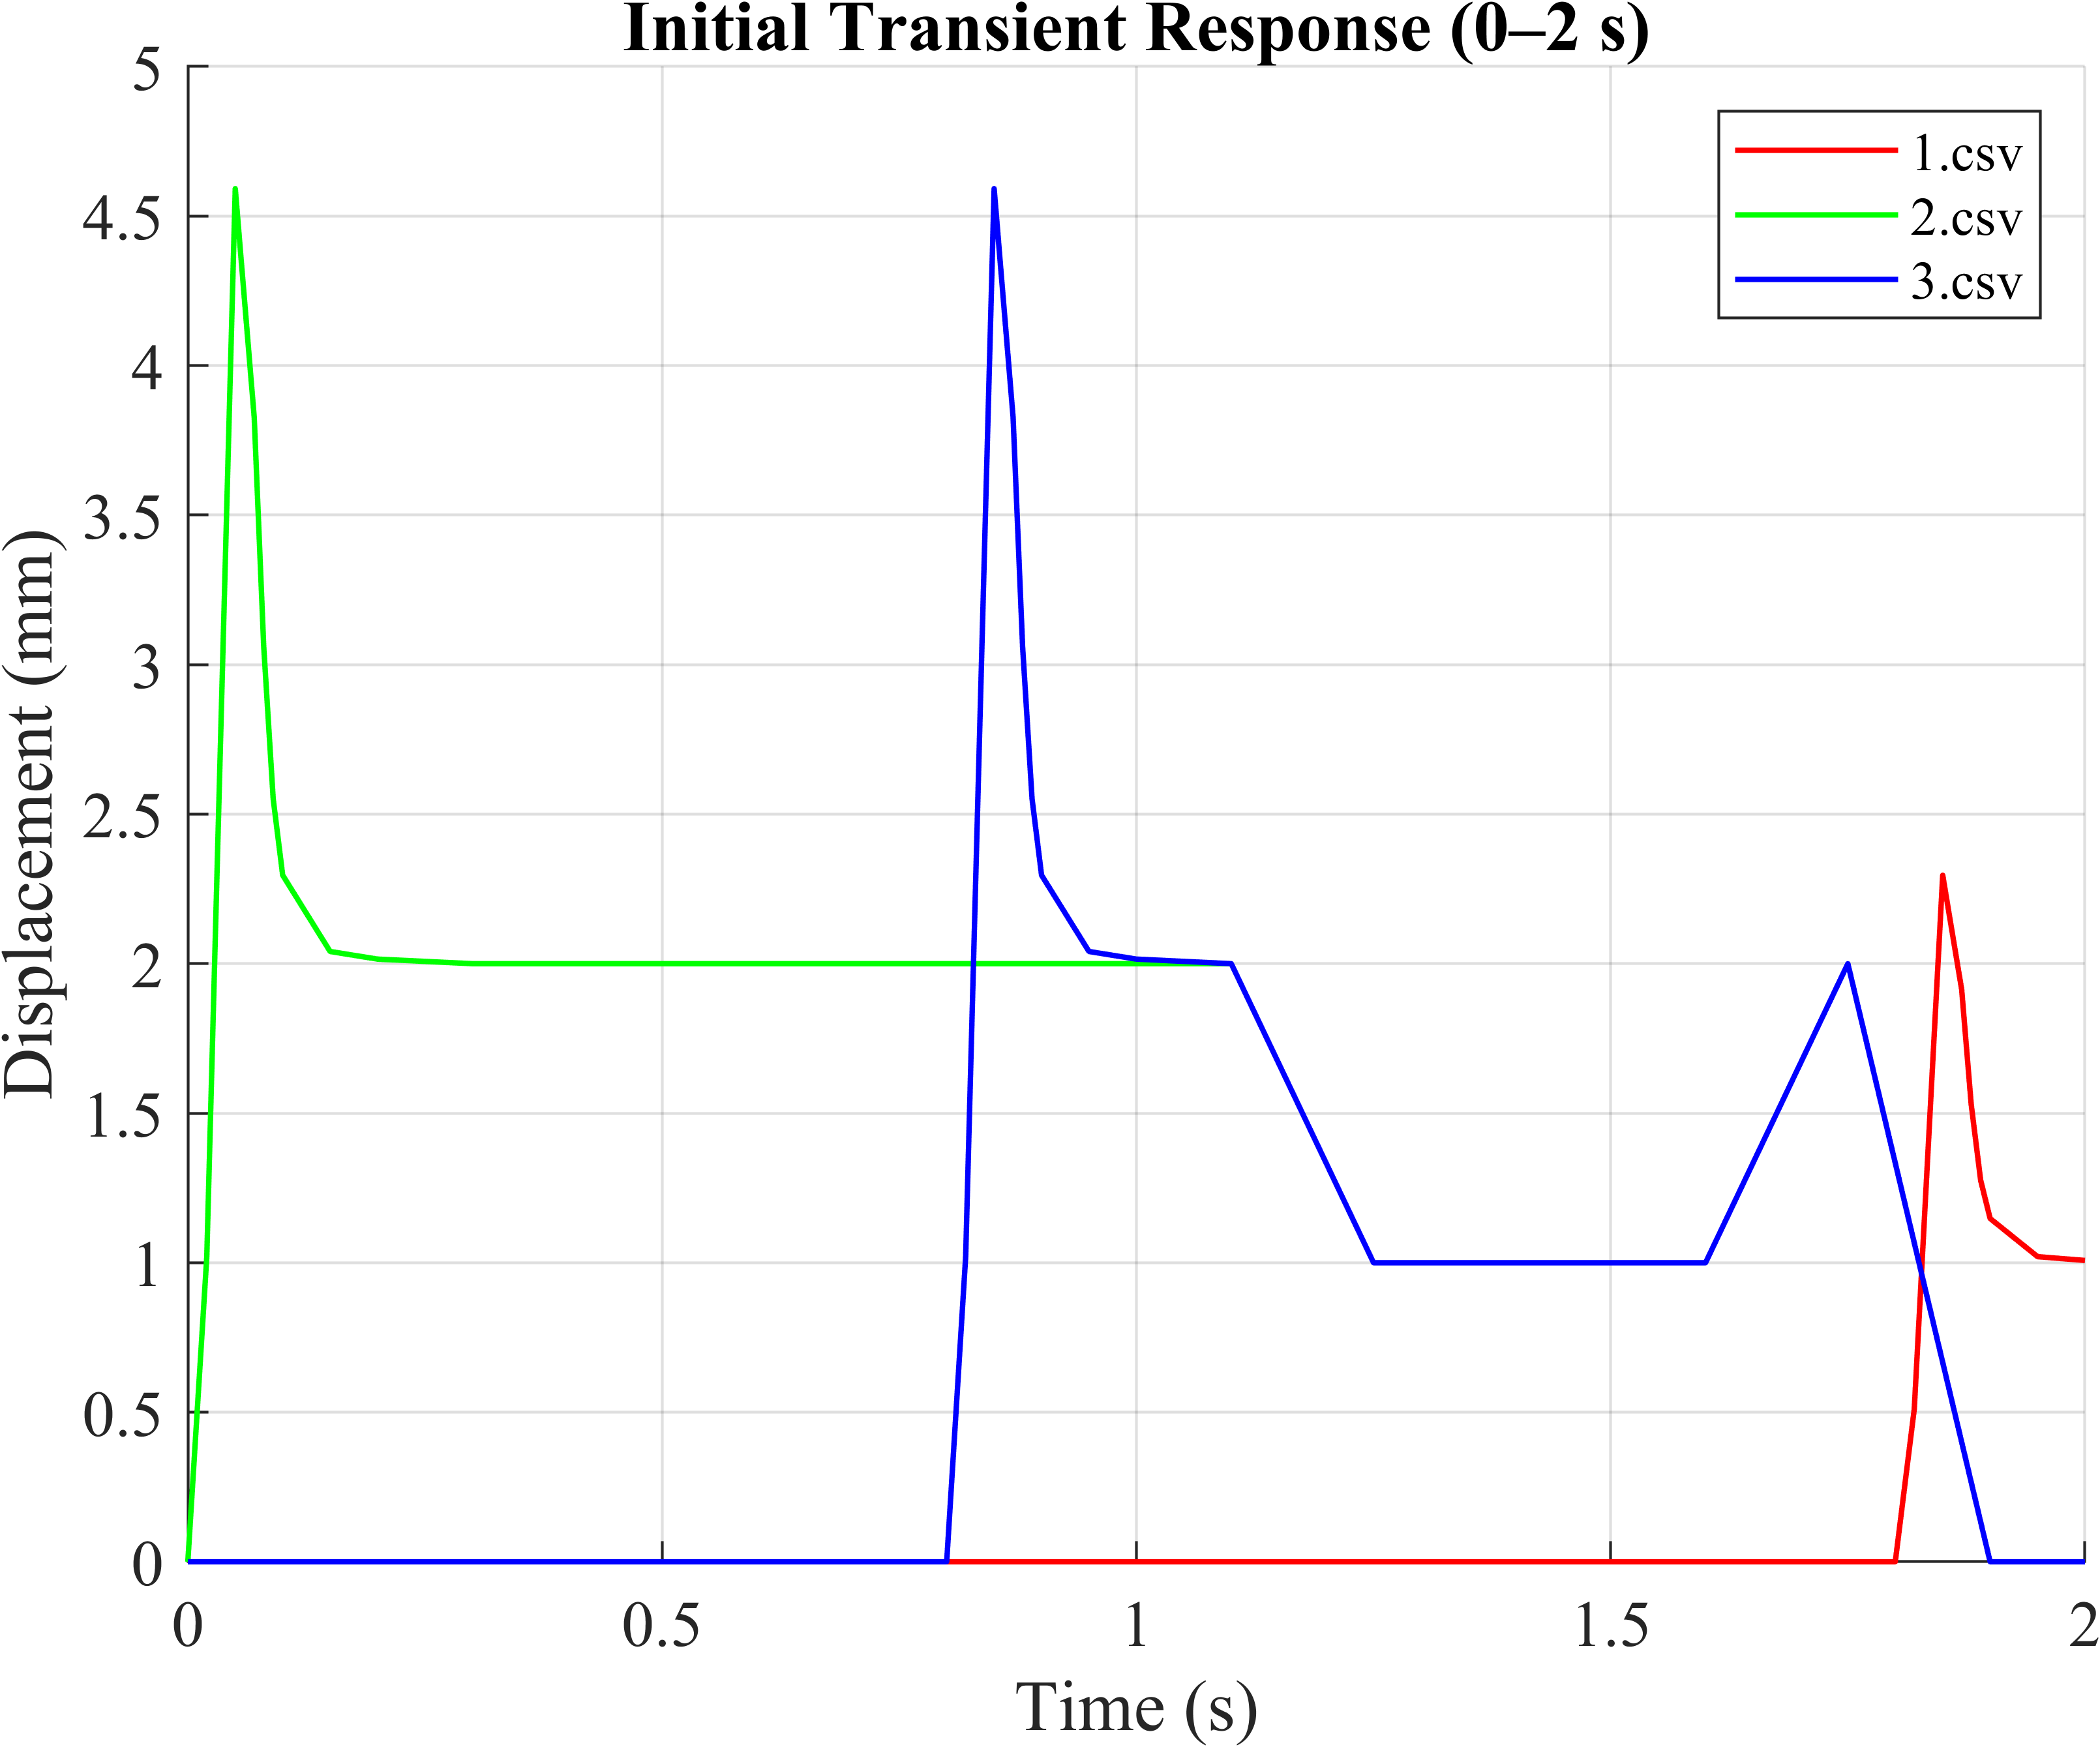
\includegraphics[width=0.48\linewidth]{pics/21_Event2.png}
    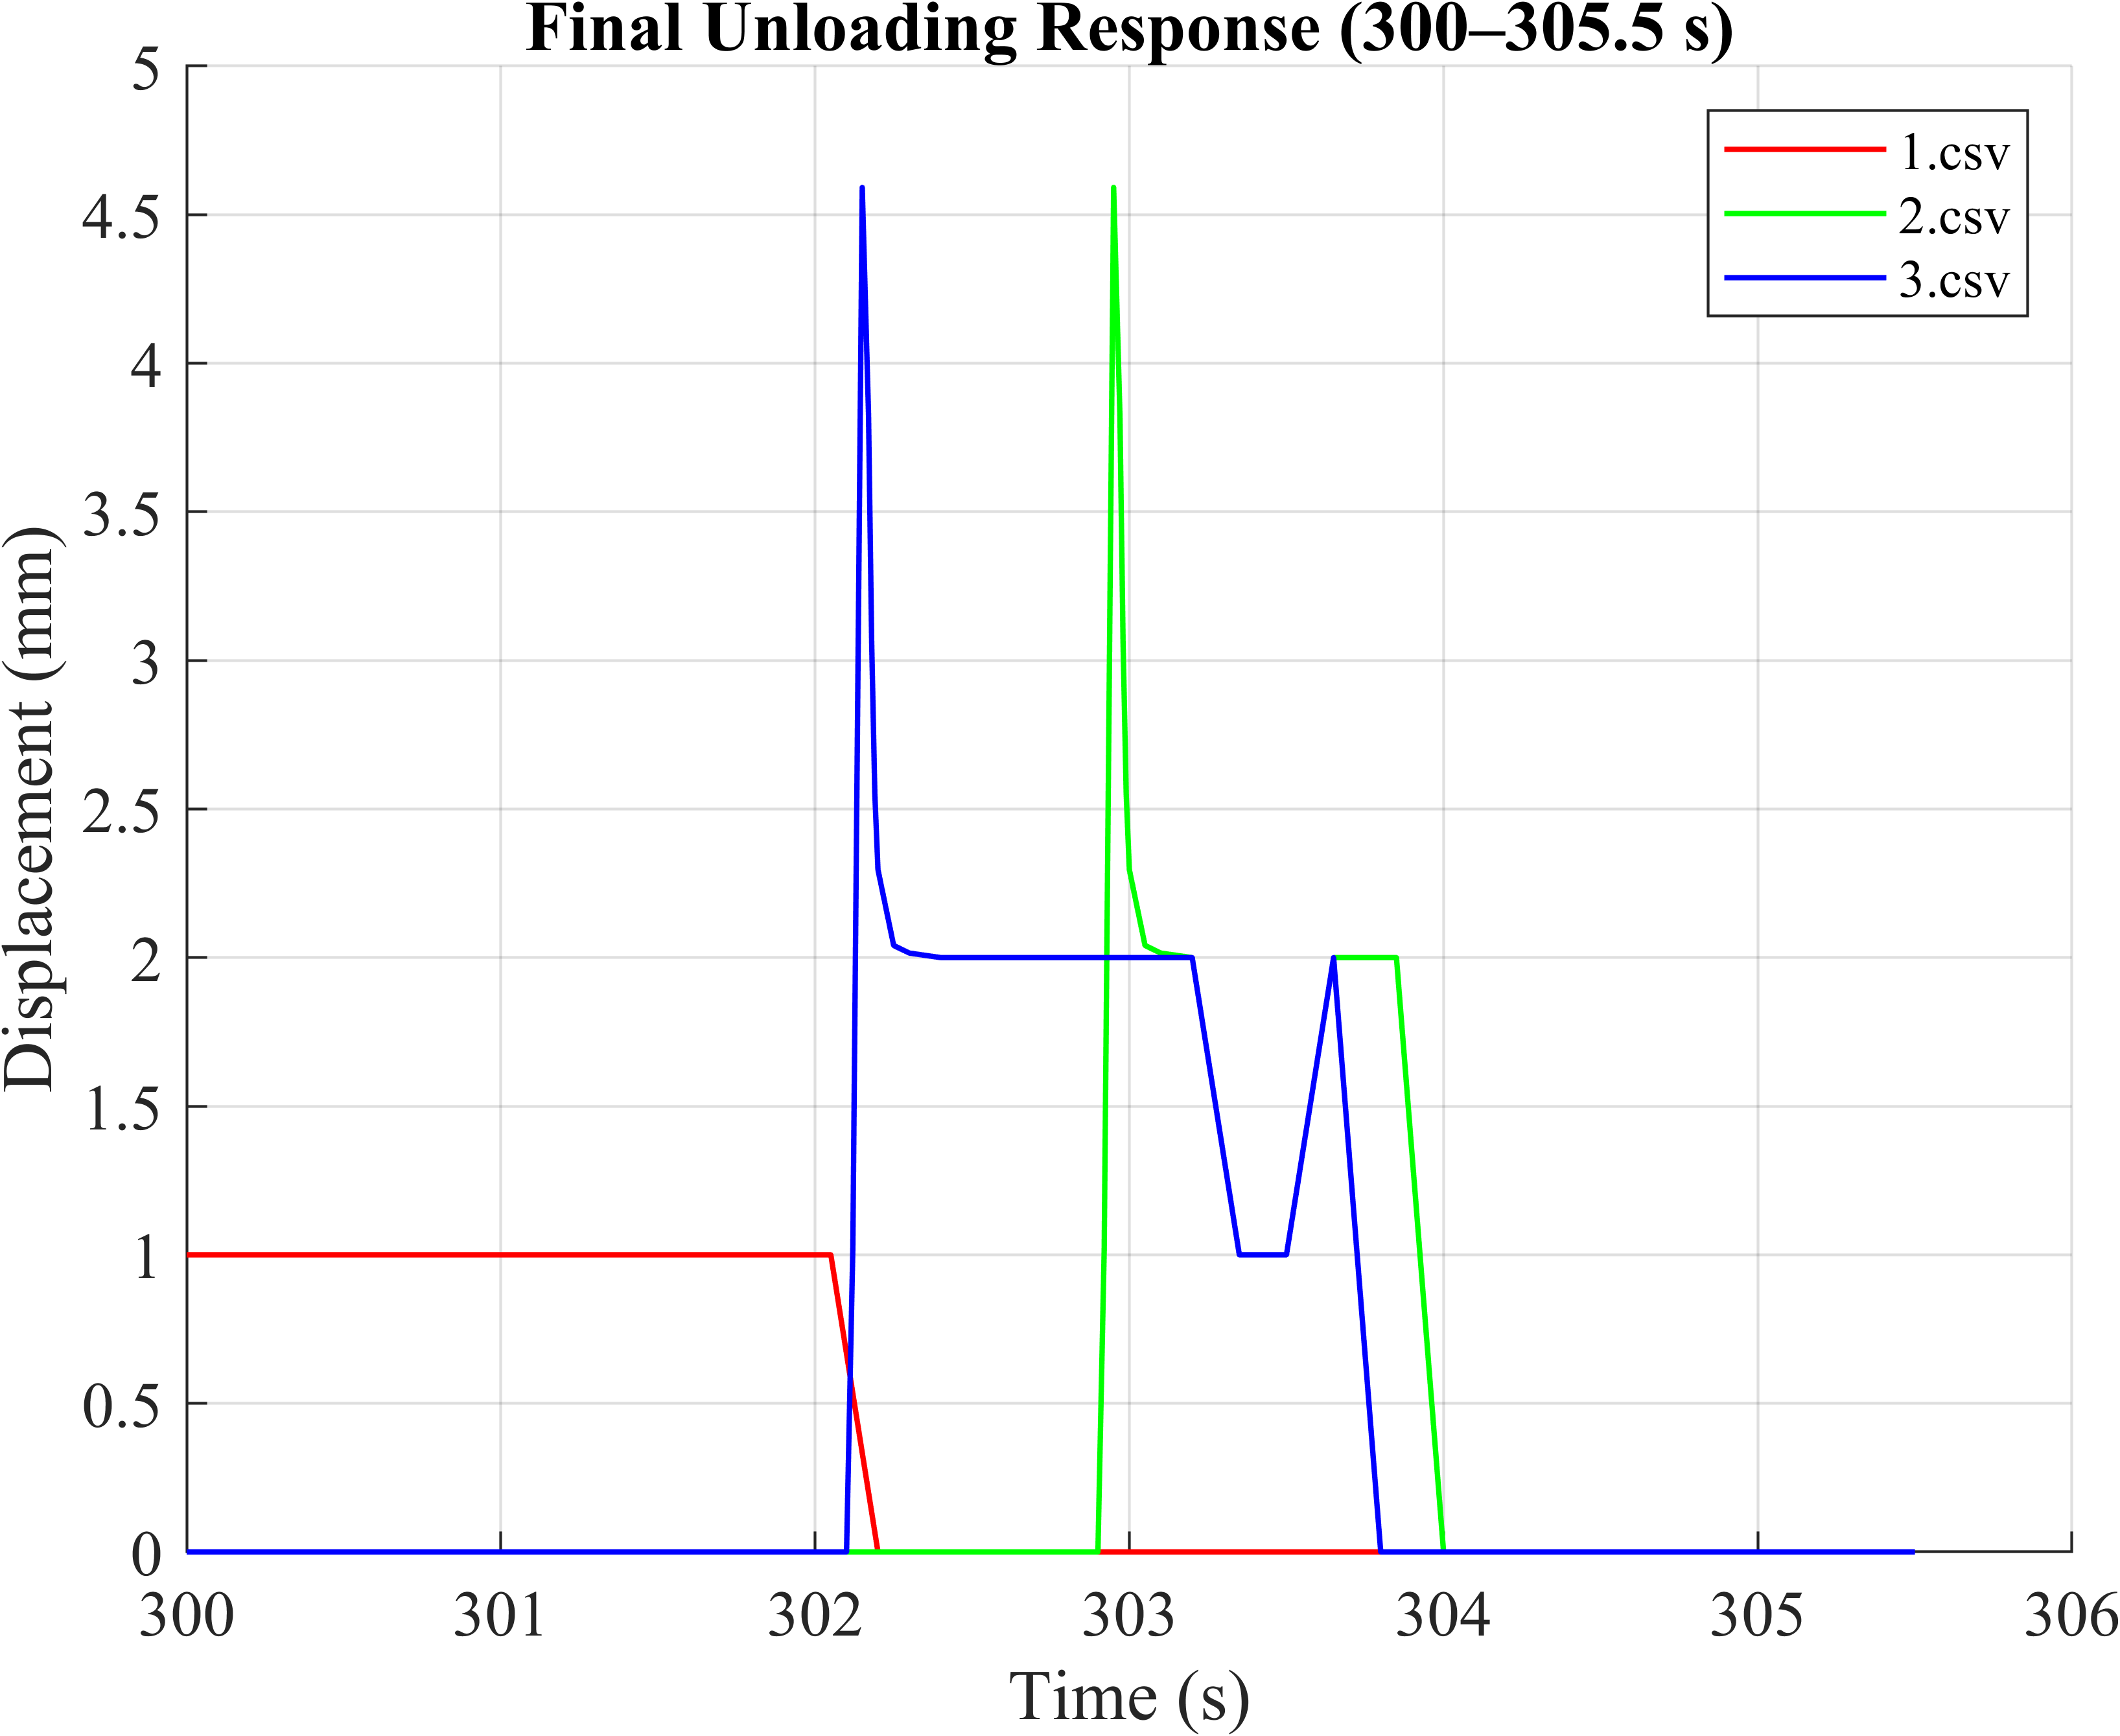
\includegraphics[width=0.48\linewidth]{pics/21_Event3.png}
    \vspace{-0.3cm}
    \caption{\small{载荷时序设置示意图}}
    \vspace{-0.4cm}
\end{figure}
\subsubsection{\heiti{载荷时序配置}}
\par{}
接着点击“HyperLife~→~Load Map”进行载荷工况的时序分配。如图21（上），打开该窗口，在右边一栏即会自动识别.h3d文件中的所有工况，这里由上至下分别为：双脚踩在顶面（同原工况一），右脚踩在第一级梯级，左脚踩在第二级梯级。现模拟的是人走上梯级，在顶面站5~min后再反着走下来的过程，因此设定幅值曲线如图21（下）所示，时序表见附件中的.csv文件。
\par{}
这种基于时序的分析方法直接将静力学分析的应力结果线性叠加应用于模型之上，因此只需要模拟这些工况出现的时序即可。因为要模拟上梯级的过程，所以只能将左右脚的两步单独分开进行静力学分析，再在这里按时间顺序分配。
\par{}
最后全选左右两栏的内容，点击最下方一栏的加号，添加到同一个事件（Event）中，并勾选该事件。
\subsubsection{\heiti{疲劳分析加载步设置}}
\par{}
点击“HyperLife~→~Evaluate Run”，在“分析位置”（Analysis Location）中选择“节点”（Nodes）即可。此时需要调用静力学仿真结果中的$\sigma_{xx}$、$\sigma_{yy}$、$\sigma_{zz}$、$\sigma_{xy}$、$\sigma_{yz}$、$\sigma_{zx}$这几个应力值，因此一开始时要在对应卡片中设置全部输出。
\par{}
分析完毕后在弹出的窗口中单击“查看当前结果”（View Current Results\dots）即可查看分析结果。
\subsection{\heiti{冲击耐碰撞分析条件设置}}
\par{}
冲击耐碰撞分析的目的主要是评估结构在极端短时高能量载荷（冲击、碰撞）下的瞬态响应和能量吸收能力，常用于汽车碰撞安全、列车耐撞性设计、产品跌落测试等情境。
\subsubsection{\heiti{冲击耐碰撞分析各项条件设置}}
\par{}
本次需要模拟一半径50~mm、长度300~mm、质量约18~kg的钢圆柱从1~m高度下落时对折叠梯顶板的冲击。首先新建分支，复制一份文件并删除无关工况与载荷等，同时，目前主流的冲击、碰撞分析求解器为ANSYS LsDyna或Altair RADIOSS，由于我们直接在安装HyperWorks时已自动安装了RADIOSS，因此点击“File~→~Solver Interface”，选择Altair RADIOSS，版本选择2025或2026即可。由于求解器不同，对于每个卡片，HyperMesh做了不同的适配，因此已有的材料、属性等需要重新配置，选择合适的即可，此处不再赘述。
\par{}
单击“3D~→~Solids~→~Cylinder”新建一圆柱，尺寸如上段设置，位置在距离顶板一定高度（约5~mm）处，属性设为P14\_SOLID，材质设置为M1\_ELAST，参数就按照通用设置（MMKS单位制下）：$\rho = 7.85{\rm E}-6$ （Rho\_Initial），$E = 210000$（E），$\nu = 0.3$（Nu）。接着为了保持圆柱的刚体性质，直接点击“Model~→~Rigids”，选择RBODY即可。
\par{}
为了模拟地面，直接点击“Model~→~Rigid Walls”新建刚性墙，通过目视调整坐标与法向后，设置如图22。注意法向一定朝上，因为碰撞只针对法向朝向的方向有效。
\par{}
\begin{figure}[H]
    \centering
    \vspace{-0.1cm}
    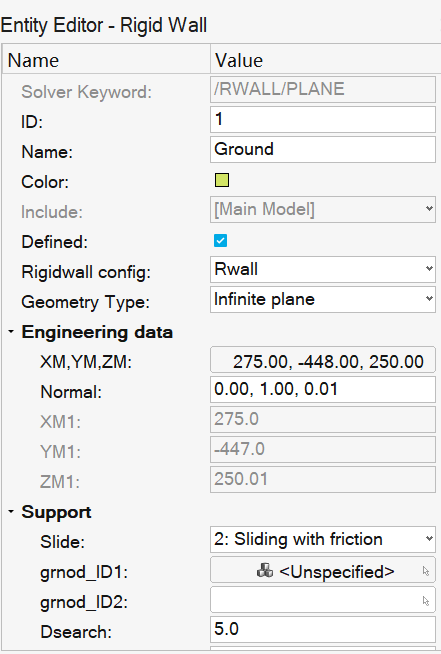
\includegraphics[height=7cm]{pics/22_Rgdwall.png}
    \vspace{-0.3cm}
    \caption{\small{地面设置示意图}}
    \vspace{-0.4cm}
\end{figure}
\par{}
接着再新建碰撞接触对，点击“Model~→~Contacts”，选择TYPE7并设置如图23，其中主面（Surf\_id (M)）为钢柱、从面为折叠梯的各部分（Grnod\_id (S)）；其他每项设置含义均为查询帮助文档得到，此处不再赘述。
\par{}
\begin{figure}[H]
    \centering
    \vspace{-0.1cm}
    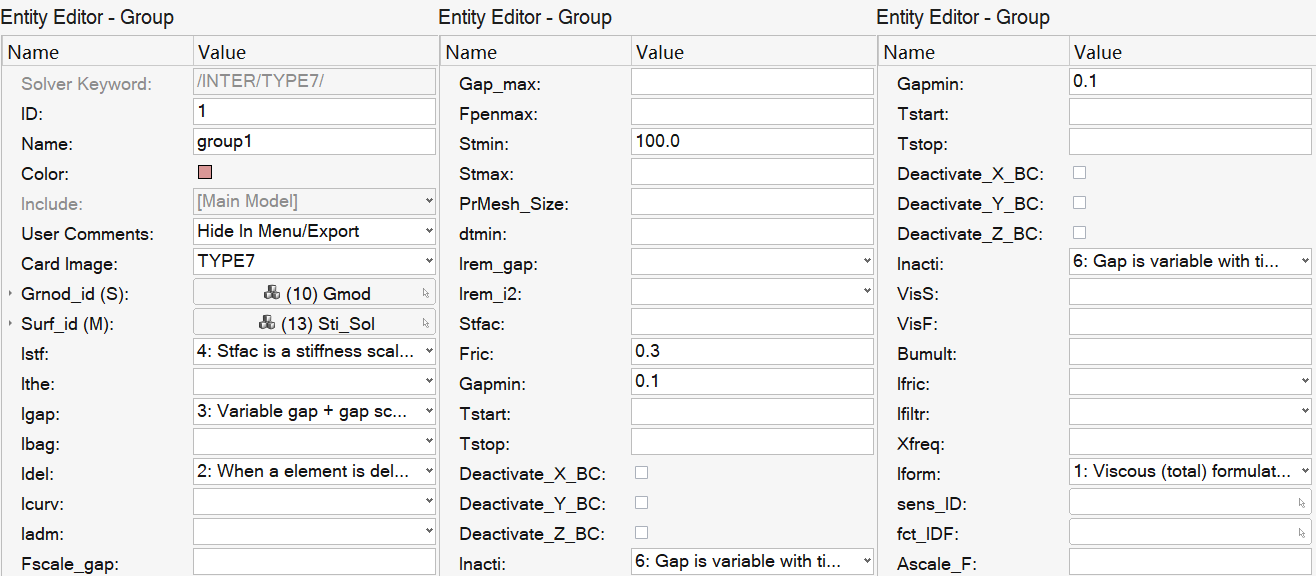
\includegraphics[width=\linewidth]{pics/23_Tp7.png}
    \vspace{-0.8cm}
    \caption{\small{碰撞接触设置示意图}}
    \vspace{-0.4cm}
\end{figure}
\par{}
再新建初始速度（INIVEL），单独给RBODY的中心创建一个集合，并直接将速度的作用对象选择为该集合，即可得整个圆柱，包括RBODY骨架及其所有网格速度均一致。再设置速度矢量为$\vec{v} = [0, -4427, 0]~{\rm mm/s}$（即1~m处自由落体速度）即可。
\subsubsection{\heiti{冲击耐碰撞分析加载步设置}}
\par{}
首先还要指定单位制。直接新建BEGIN\_CARD，将长度、质量、时间单位按MMKS单位制（mm、kg、s）设置即可。
\par{}
点击“Analyse~→~Run~→~Engine File Assistant”新建引擎文件，此时会自动弹出图24所示的界面。勾选创建引擎文件（Create Engine File），终止时间（Termination Time）设为0.05，动画输出频率（Animation Output Frequency）设置为0.0002，时间历史输出频率（Time History Output Frequency）设置为0.00002即可。这些值决定了动画的时长、帧率等，设置好后软件会自动生成一系列卡片，保持默认即可。
\par{}
\begin{figure}[H]
    \centering
    \vspace{-0.1cm}
    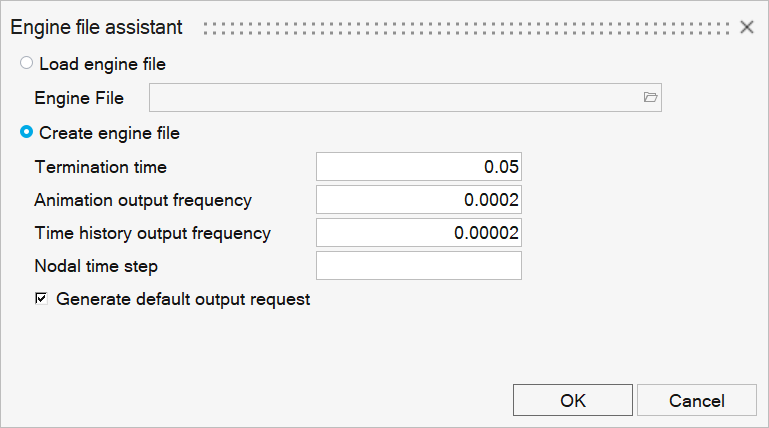
\includegraphics[width=0.7\linewidth]{pics/24_Timeset.png}
    \vspace{-0.3cm}
    \caption{\small{引擎文件设置示意图}}
    \vspace{-0.4cm}
\end{figure}
\par{}
在本次分析中，沙漏能对能量影响尤其大。因此在生成的H3D/ELEM卡片中还要勾选沙漏能输出（HOURGLASS），以监视沙漏能影响。
\par{}
最后点击“File~→~Export~→~Solver Deck”输出.rad格式的求解文件进行求解即可。
\subsection{\heiti{小结}}
\par{}
所有加载步都设立完毕后，由于我们在网格划分时已经进行过网格质量检查，在Optistruct中就不需要再次进行了。故应在模型浏览器（Model Browser）中新建卡片（Cards）。在新建窗口中选择“参数”（PARAMS）卡片，点击设置其为激活状态，再点击勾选其中的“网格质量检查”（CHECKEL），并将下拉菜单内容设置为“不检查”（NO），以避免进行额外的网格质量检查而报错。
\par{}
同时，若想要观察仿真时的更多程序信息与硬件性能等信息，可以新建“屏幕”（SCREEN）卡片，点击设置其为激活状态，并将其唯一的下拉菜单栏设为“输出”（OUT）。
\par{}
接着点击“Analyze~→~Run”保持默认设置直接输出.fem文件，HyperMesh会自动输出文件并启动Compute Console 2026（即Optistruct求解器命令行），在其中设置栏输入“-nt xx”启用CPU中的多核（如-nt 16就是16核）并行计算，“-gpu cuda”开启GPU CUDA加速（仅英伟达显卡）。此外，如果遇到计算机内存不足而出现报错的情况，可以输入“-len xxxx”（指定内存限制，单位MB），将内存占用限制在某个值，或“-core OUT”，将溢出内容存储与磁盘。
\par{}
如果想仅针对某个工况进行分析，可以使用Visual Studio Code打开.fem文件，删除无关的工况信息、仅保留目标加载步及其前置加载步即可。
\par{}
完成上述所有内容后即可点击运行（Run）按钮进行仿真分析。
\newpage{}
\section{\heiti{仿真结果及其分析}}
\par{}
\textcolor{red}{\textbf{所有输出结果图均见文末附图。}}
\subsection{\heiti{静态特性分析结果}}
\par{}
针对两个工况，分别展示其应力分布云图、位移分布云图、应力极值、位移极值。
\subsubsection{\heiti{工况一}}
\par{}
如附图1.1，应力极值为$\rm 40.42~MPa$，且$\rm 3~MPa$以上的应力分布在顶板和前支撑连接处螺栓附近。结合实际推测该部分应力集中，但极值处也可能发生应力奇异现象，有待验证。
\par{}
如附图1.1，位移极值为$\rm 1.081~mm$，分布在顶板中心位置；可发现$\rm 0.2402~mm$以上的位移几乎都出现在连接杆及其上方的其他部件处，符合预期。
\par{}
此外，应力分布、位移分布轻微不对称，这主要是因为折叠梯前支撑结构不对称（Z字连接）。
\subsubsection{\heiti{工况二}}
\par{}
如附图1.2，应力极值为$\rm 19.25~MPa$，且$\rm 2~MPa$以上的应力分布在螺栓和梯级与后支撑连接处附近。结合实际推测该部分应力集中，但极值处也可能发生应力奇异现象，有待验证。
\par{}
如附图1.2，位移极值为$\rm 1.242~mm$，分布在第二级梯级受力区域中心；可发现$\rm 0.2760~mm$以上的位移几乎都出现在两梯级受力区域，符合预期。
\par{}
此外，应力分布、位移分布明显不对称且第二级位移整体偏大，这主要是因为载荷施加本身就不对称，同时第一级的位移叠加在第二级上，因此出现此种分布特征。
\subsection{\heiti{动态特性分析结果}}
\subsubsection{\heiti{模态分析}}
\par{}
对前$\rm 200~Hz$的所有模态进行分析，由输出的.out文件得共有502阶模态，详见附件中的Case02.out或Case02.txt文件。
\par{}
使用MATLAB对模态增长进行绘图（程序文件见 Case02.m），如附图2.1。这里由于模态广义质量前处理时选择了归一化，均为1，这里省略绘图。
\par{}
不难发现模态数随频率近似线性递增、中后期略微放缓，即可视为均匀分布。模态特征值（Eigenvalue）与广义刚度（Stiffness）相同，近似成凹二次函数形式递增，表明越高阶的模态下结构抵抗变形的能力越强，要激发同样大小的振型位移，需要更高的能量输入。因此推测当处于较高频率范围——如前处理时因空间不足而舍去的$\rm 1990$~\textasciitilde~$\rm 2100~Hz$——时，较难发生明显共振。
\par{}
针对更贴近人自身频率的较低频段$\rm 0$~\textasciitilde~$\rm 50~Hz$，附图2.2列出了常见的几种振动部位（幅度放大50倍）。从左到右、从上到下排列，依次为第1、2、4、5、6、12号模态，分别代表顶板整体平动振动、前支撑Z字连接振动、前支撑扭转振动、后支撑弯曲振动、连接杆与前支撑弯曲振动、梯级和顶板弯曲振动。
\par{}
据目测估计，$\rm 0$~\textasciitilde~$\rm 50~Hz$频段内的振动模态中，最频繁出现较明显振动的部件为前支撑Z字连接与顶板靠前支撑的区域，其次为连接杆与梯级，这些地方针对低频振动应增加刚度或阻尼。
\subsubsection{\heiti{频率响应分析}}
\par{}
经过频响分析，得16个关键点的位移响应如附图2.3，其中，前三张分别为$x$，$y$，$z$轴方向上的位移响应幅值；后三张分别为$x$，$y$，$z$轴方向上的加速度响应幅值；速度响应介于两者之间，此处省略。其中可以看到同一方向的位移响应幅值几乎与加速度响应幅值保持相同趋势，即集中在前10~Hz内，但绝对值不同，符合对三角函数求二阶导的规律（$a_{x} = \ddot{x} = {\rm d}x/{\rm d}t$）。
\par{}
接着详细观察各节点情况。附图2.3图例中的各节点编号与位置对应关系如下表：
\begin{table}[htbp]
    \centering
    \songti
    \begin{tabular}{|c|c||c|c|}
        \hline
        \heiti{节点编号} & \heiti{位置描述} & \heiti{节点编号} & \heiti{位置描述} \\
        \hline
        12227        & 顶板中间偏后       & 154949       & 第二级梯级中心      \\
        \hline
        46180        & 第一级梯级中心      & 634368       & 右连接杆中心       \\
        \hline
        64172        & 后支撑右侧中心      & 642271       & 左连接杆中心       \\
        \hline
        102552       & 后支撑左侧中心      & 678313       & 前支撑右侧中心      \\
        \hline
        106767       & 顶支撑右侧中心      & 702907       & Z字支撑上杆中心     \\
        \hline
        110787       & 顶板中间偏前       & 707711       & Z字支撑中杆中心     \\
        \hline
        113642       & 顶支撑左侧中心      & 709030       & Z字支撑下杆中心     \\
        \hline
        114396       & 横条中心         & 731310       & 前支撑左侧中心      \\
        \hline
    \end{tabular}
\end{table}
\vspace{-0.2cm}
\par{}
由附图2.3可知，$x$方向上在3~Hz与5~Hz附近，左右连接杆振动最为剧烈；$y$方向上在7~Hz和8~Hz附近，顶板中心振动最为剧烈；$z$方向上在3~Hz附近，Z字支撑中间斜杆振动最为剧烈。这些结果都符合日常认知，尤其是$y$方向上的，类似于静态分析时的结果，总是顶部中心（也是作用区域中心）位移最大。
\subsubsection{\heiti{瞬态响应分析}}
\par{}
如附图2.4.1与2.4.2，瞬态分析结果中，力的瞬间峰值使得梯级产生了振动，图中便是每次振动达到最大值时的图像（前9次、后9次）；完整的振动动画请见附件中的Case0503.gif文件。
\par{}
可见瞬时力的作用使得第一级梯级发生了较为剧烈的振动，最高峰值为6.525~mm，远大于静态特性分析时该区域的结果。根据时间戳计算振动周期，可得振动周期约为0.16~s，振动频率约为6.25~Hz。查询模态分析结果发现在6.25~Hz附近，的确存在数个梯级的振动模态，包括模态11（约6.17~Hz）、模态12（约6.25~Hz）、模态14（约6.31~Hz），因此推测是加载力激起了其中某个模态的振动。同时发现经过了5~s，振动虽有衰减，但衰减幅度较小，推测是阻尼设置0.06过小导致。
\par{}
同时，如附图2.4.3，每次振动，位移最大的区域在梯级中心附近，但第一次振动是从力的作用区域发起的，后传导至中心引起振动，还传到至梯级的左半侧，呈现出波的形态；在振动后期由于能量传递，也引起了其他部件的振动。当然，由于是欠阻尼状态，振动衰减慢，不太符合现实；但振动传递确实是客观存在的，而在仿真条件下，仿真结果也是符合物理规律的。
\par{}
对于应力分布，类似于静态特性分析中的工况二，集中分布在梯级与后支撑的连接处，同时随着振动而周期性变化，并无其他特殊之处，故省略分析。
\subsubsection{\heiti{随机振动分析}}
\par{}
结果文件中，我们得到了加速度、位移和应力的PSD值和RMS值，其中，PSD值仅在每个FREQi取值的频率下有效，RMS值仅在最终输出的频率有效值（RMS over frequencies）中有效。
\par{}
由于RMS值满足：
\begin{equation*}
    RMS = \sqrt{\mathbb{E}[X^2] - \mu^2} = \sigma ~~~~(\mu = 0)
\end{equation*}
因此有：
\begin{equation*}
    3\sigma = 3RMS ~~~~(\mu = 0), ~~~~~~~~P(|X| \leq 3\sigma) = 99.73\%
\end{equation*}
即元素的对应取值有99.73\%的概率落在$3\sigma$范围内。
\par{}
如附图2.5，振动加速度RMS值为1.244~$\rm m/{s^2}$，则$3{\sigma}_a = 3.732 {\rm m/{s^2}}$，主要分布在各长条形部件中部（左上图），位置与幅值均符合日常认知；振动位移RMS值为1.193~mm，则$3{\sigma}_d = 3.579$~mm，主要分布区域同加速度（右上图），位置与幅值也符合日常认知；振动应力RMS值为15.76~MPa，则$3{\sigma}_s = 47.28$~MPa，推测是某连接处出现应力奇异导致的，其他大部分主干区域应力均在1~MPa以下（左下图），远低于许用值上限的15\textasciitilde17~MPa\textsuperscript{\textcolor{red}{\cite{ref2}}}，较高应力区域通常分布在连接处，但除极少数可能存在应力奇异的元素外几乎不存在超过3~MPa的点，针对此类区域应做好减振措施，避免振动造成的疲劳损伤。
\par{}
\subsection{\heiti{稳定性分析结果}}
\subsubsection{\heiti{工况一}}
\par{}
工况一在$BLF \in [0,~100]$区间内共有21个失稳模态，详见附件中的Case03.out或Case03.txt文件。如附图3（上左、上右），这是工况一下的前两个失稳模态，也是$BLF$最小的两个失稳模态，可见分别是两侧连接杆件发生了第一类质变失稳，且由于结构、载荷的近似对称性，两模态的$BLF$也近似相等。但此时$BLF$分别等于约37.2与38.1，临界载荷分别为约$\rm 0.81~MPa$与$\rm 0.83~MPa$，对应人的体重在$\rm 2000~kg$以上，明显已经在正常使用范围之外，因此判断日常使用时，不会发生失稳现象。
\par{}
\subsubsection{\heiti{工况二}}
工况二在$BLF \in [0,~100]$区间内共有14个失稳模态，详见附件中的Case03.out或Case03.txt文件。如附图3（下左、下右），这是工况二下的前两个失稳模态，也是$BLF$最小的两个失稳模态，可见仍然是两侧连接杆件发生了第一类质变失稳，且由于载荷的不对称性，两模态的$BLF$也不相等。但此时$BLF$分别等于约33.5与51.5，临界载荷分别为约$\rm 1.40~MPa$与$\rm 2.15~MPa$，对应人的体重在$\rm 2000~kg$以上，明显已经在正常使用范围之外，因此判断日常使用时，不会发生失稳现象。
\subsection{\heiti{结构优化分析结果}}
\par{}
仅经过5次迭代，优化就达到程序所默认设定的收敛要求，优化结束，迭代过程详见附件中的Case04.out文件。设定显示阈值为0.2，得经拓扑优化，被优化区域大致沿对角线被分为密度为0的部分与其他部分，且由于挤出设置的约束，垂直于$x$轴的截面基本一致，如附图4。
\par{}
通过HyperMesh中的“Optimize~→~Tools~→~OSSmoth”功能，还可对输出结果进行平滑处理，但这里由于有较多网格，处理起来极其缓慢（8小时后依旧无响应，比求解时间还长），遂放弃。
\subsection{\heiti{疲劳分析结果}}
\par{}
如附图5，由于HyperLife没有导出报告功能，因此只能采用截图的方式。其中，左上图为疲劳寿命图，可见模拟工况下最低疲劳寿命为约16310次，其他区域的寿命均几乎为永久；左下图的疲劳破坏区分布于梯级与后支撑连接处以及前支撑与顶支撑螺栓连接处，最大裂纹尺寸约为2.098~mm，且只有踩踏侧存在，这是因为仿真中只踩了一侧，现实中可能根据使用者习惯有不同结果，若使用者没有按仿真中的规律只踩某侧，则两侧都会出现疲劳损伤。
\par{}
需要注意的是，该结果过于理想化，未考虑气候条件、生物条件等对木材的侵蚀，实际使用寿命一定短于预计值。
\subsection{\heiti{冲击耐碰撞分析结果}}
\par{}
如附图6，这是碰撞仿真结果。由于碰撞分析需要较大内存，因此到约0.0325~s，即约65\%时程序崩溃。由于此前做了各种尝试，很难在抑制沙漏能、控制断裂与网格删除、控制内存占用和计算时间内取得平衡，因此选择性展示较好的结果以及存在问题的结果，并推测耐碰撞情况。完整动画请见附件中的Case07.gif。
\par{}
如前3张图，这是进行到一半的正常结果（圆柱已隐藏）。可见圆柱下落后碰撞接触生效，同时折叠梯顶板中部顺着圆柱方向出现凹陷（第1、2张），且最后展现出疑似裂纹的网格形态（第3张），这说明钢柱极有可能已经压溃顶板。
\par{}
第4张图是某次仿真中沙漏能的示意图，几乎完全出现在圆柱体的边缘，仿真时显示能量误差达到49.6\%，仿真结果不可信。这表明可能由于RBODY的链接导致沙漏能异常，删除RBODY并直接将速度赋予圆柱即可解决该问题（前3张就是删除后仿真得到的结果）。
\par{}
第5张图是某次仿真时添加网格失效删除的结果，目前尚未探索清楚删除应变阈值的确切值，但可以确定的是，应变达0.3时删除仍然过快。这也暗示了钢柱接触瞬间，折叠梯顶板所受瞬时力过大，导致应变巨大而瞬间折断。
\par{}
综上，推测折叠梯无法抵抗约18.5~kg的钢柱从1~m处下落时的冲击。
\newpage{}
\section{\heiti{结果分析评价}}
\par{}
下面针对有限元分析结果进行评价。
\subsection{\heiti{静态特性分析结果评价}}
\par{}
静态特性分析几乎是最为准确与可靠的，虽然其工况较为理想，但且与生产实际结合较为紧密，能基本确定实际使用时的受力情况，找出危险点等。当然也可能存在应力奇异的现象，可以细化网格进一步探究；同时材料参数设置存在一定的估算成分，可能造成一定误差，实际作业时应先对材料做力学性能测试。
\subsection{\heiti{动态特性分析结果评价}}
\par{}
对于模态分析，个人认为模态过于密集了，但整体反映的模态情况较符合认知，只考虑低频模态的情况下，仿真得到的模态应该会大量出现。
\par{}
对于频率响应分析，由于计算机性能限制，故位移响应图像刻度较稀疏，但仍然可以反映一定的趋势，且和模态分析可以相互印证。
\par{}
对于瞬态响应分析，梯级振动时间过长，推测是阻尼不够；同时还发现瞬态载荷激起了某些个模态的振动，因此也可以印证模态分析结果。
\par{}
对于随机振动分析，同样由于性能限制，FREQi只选择了固定步长的FREQ1，但相比之下FREQ3更精确，而结果总的来说依旧符合常识，同时也为减振防疲劳提供了一定指导。
\subsection{\heiti{稳定性分析结果评价}}
\par{}
稳定性分析结果的模态出现位置基本符合猜测，但其值疑似偏大；当然也可以理解为“正常使用时不会发生屈服，发生屈服前木材已被压坏”。
\subsection{\heiti{结构优化分析结果评价}}
\par{}
拓扑优化结果总的来说收敛过快，虽然符合约束但没有出现网络上很多教程里的那种奇特的拓扑结构，考虑到性能限制，在进行数次（十次以上）尝试后还是放弃了。
\subsection{\heiti{疲劳分析结果评价}}
\par{}
疲劳分析结果较为符合认知，如踩踏梯级一定会在梯级与后支撑连接处产生疲劳裂纹；但实际结构与简化结构还是存在差距，因此出现裂纹的部件待讨论；并且现实中考虑环境因素的影响，实际使用寿命必定低于仿真结果。同时由于HyperLife自带的材料库中没有各向异性材料的模板，只能用各向同性材料，因此这也会造成一定误差。
\subsection{\heiti{冲击耐碰撞分析结果评价}}
\par{}
对于冲击耐碰撞分析，在基于多轮调参后输出了一个基本可信的结果，但很可惜由于某些设置不完全正确、或计算机内存不足，导致时间步在碰撞发生一定时间后坍缩、最终求解器跑飞或崩溃，但好在得到了一半结果，得以一窥碰撞后的部分状态。
\par{}
\quad{}
\par{}
\section{\heiti{总结}}
\par{}
本次作业中，我使用了Altair公司的多种软件或程序，包括HyperMesh、Hyperview、HyperLife、Optistruct求解器、RADIOSS求解器等，锻炼了从静态到动态力学仿真的前处理、后处理以及结果分析能力，也学会了分析错误日志，并按图索骥修正错误。
\par{}
当然我也遇到过很多困难。首先就是电脑内存不足、硬盘空间不足等导致的计算缓慢或存储溢出，这些基本都通过简化求解的方式成功解决。其次是网络上的相关资料极其繁多，从视频到文档、从老界面到新界面，浏览需要时间、理解也需要时间，在这个筛查信息、吸收知识的过程中，我不仅按照着教程的指引调整求解文件，还尝试自己探索，虽然付出了很多时间代价，但一切都值得。
\par{}
同时AI的使用也带给我极大的便利。帮助文档英语专用词汇较多，一个个查十分费时，自动翻译又不够准确，直接复制粘贴给AI，让其来解释并提出建议，自己再去核实与尝试，这个效率比单打独斗提升不少。同时网络上有些方面的资料较为稀缺，如HyperLife和RADIOSS前处理的过程，由于网络上针对疲劳分析与碰撞分析大都使用ANSYS系软件，虽然我也可以安装，但电脑存储空间实在不够了；在网上寻找散装资料有太耗时，因此只能求助AI帮我寻找资料，并逐一核实。AI还有一个重要作用是分析日志，当出现报错或警告时，通知本地运行的AI Agent直接读取日志文件可以快速定位错误，十分便利。
\par{}
总的来说，虽然本算例十分巨大、计算时存在诸多问题，但作为练习作业，从一开始的一无所知、对复杂的界面不知所措，到后期的熟练操作，我认为该作业极大地提升了个人在有限元仿真方面的能力，为我今后的学习或工作打下了基础。
\begin{flushleft}
    \begin{small}
        \begin{thebibliography}{99}
            \bibitem{ref1}CRAFTSMANSPACE. Folding step ladder plan[EB/OL]. 2019-10-17[2026-04-29]: 3. \href{https://www.craftsmanspace.com/sites/default/files/free-plans-pdf-files/Folding%20step%20ladder%20plan.pdf}{\textcolor{blue}{https://www.craftsmanspace.com/sites/default/files/free-plans-pdf-files/Folding\%20step \%20ladder\%20plan.pdf}}.
            \vspace{-3mm}
            \bibitem{ref2}江西省土木建筑学会. 《木结构设计标准》（GB 50005-2017）[EB/OL]. 2021-11-05[2026-05-01]: 144. \href{https://ceasjx.com/articles/content_2170.html}{\textcolor{blue}{https://ceasjx.com/articles/content\_2170.html}}.
        \end{thebibliography}
    \end{small}
\end{flushleft}
\newpage{}
\par{}
\begin{figure}[h]
    \centering
    \phantomsection
    \addcontentsline{toc}{section}{附图}
    \vspace{-0.1cm}
    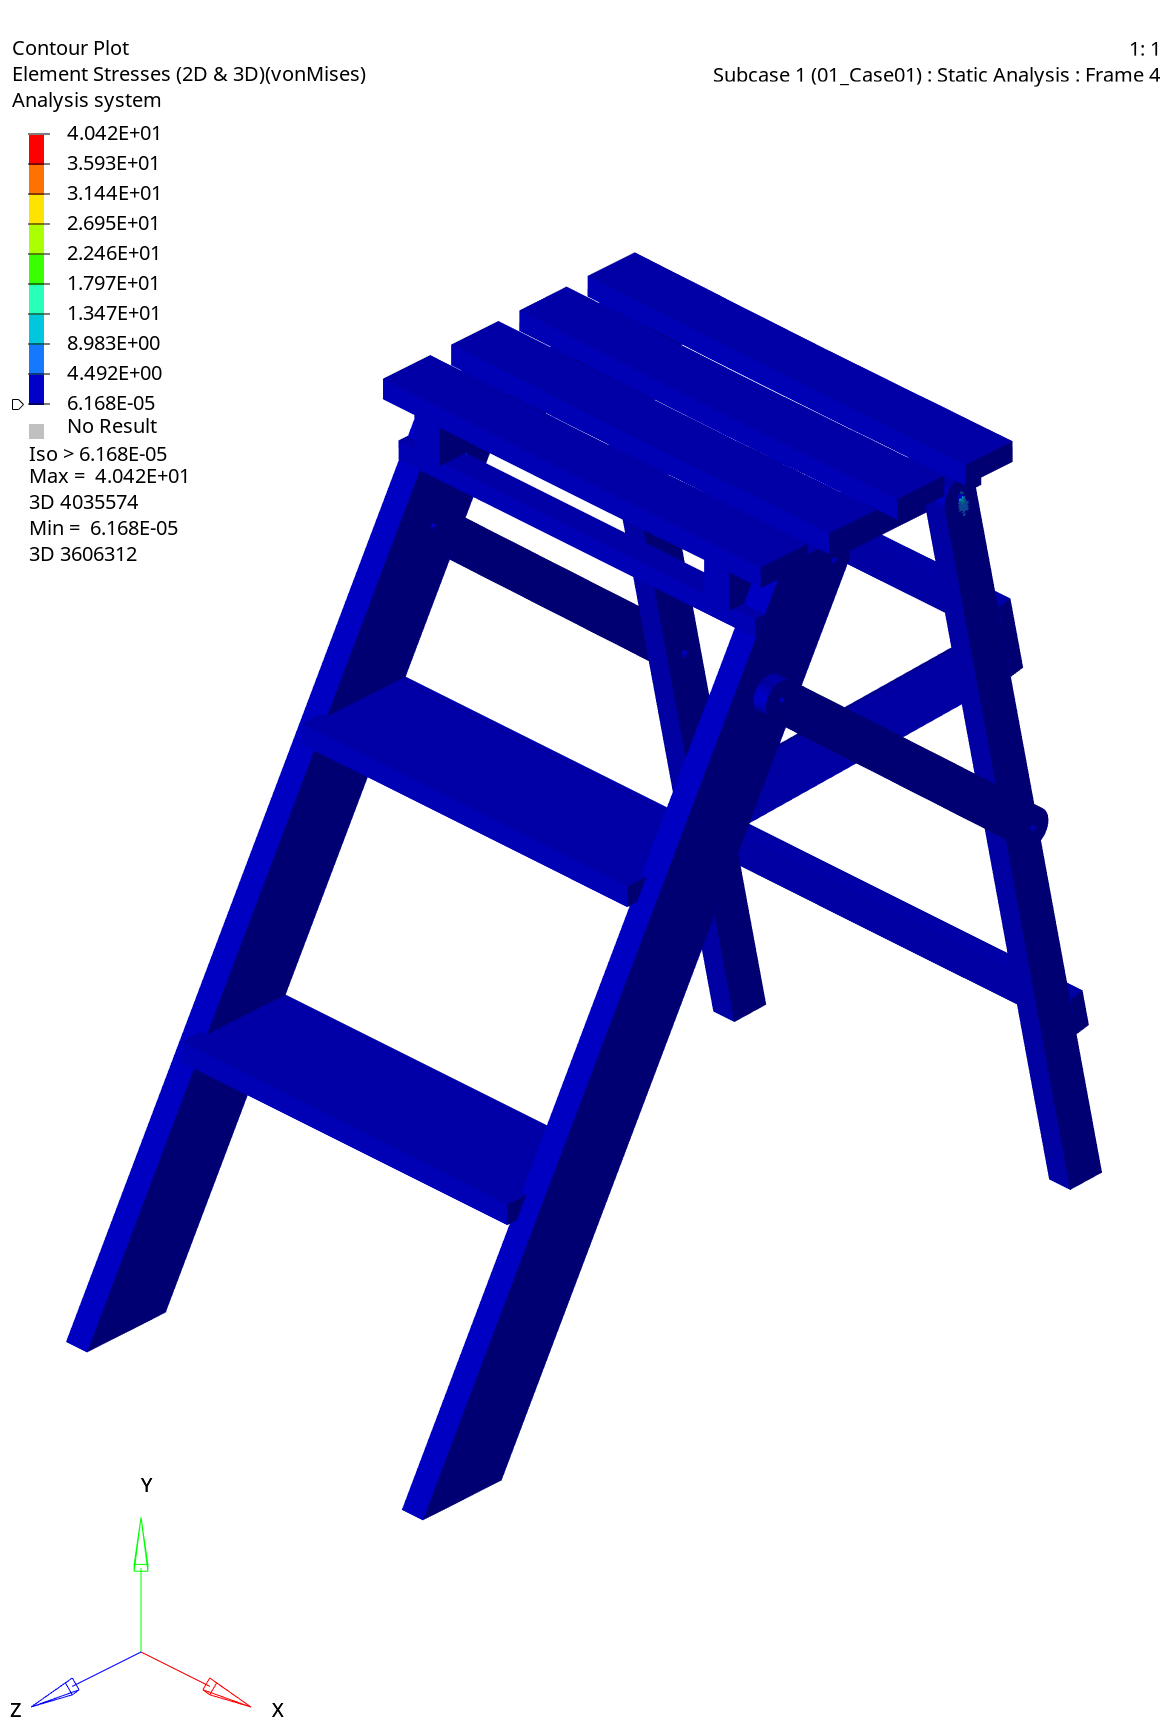
\includegraphics[width=0.48\linewidth]{pics/C010101.png}
    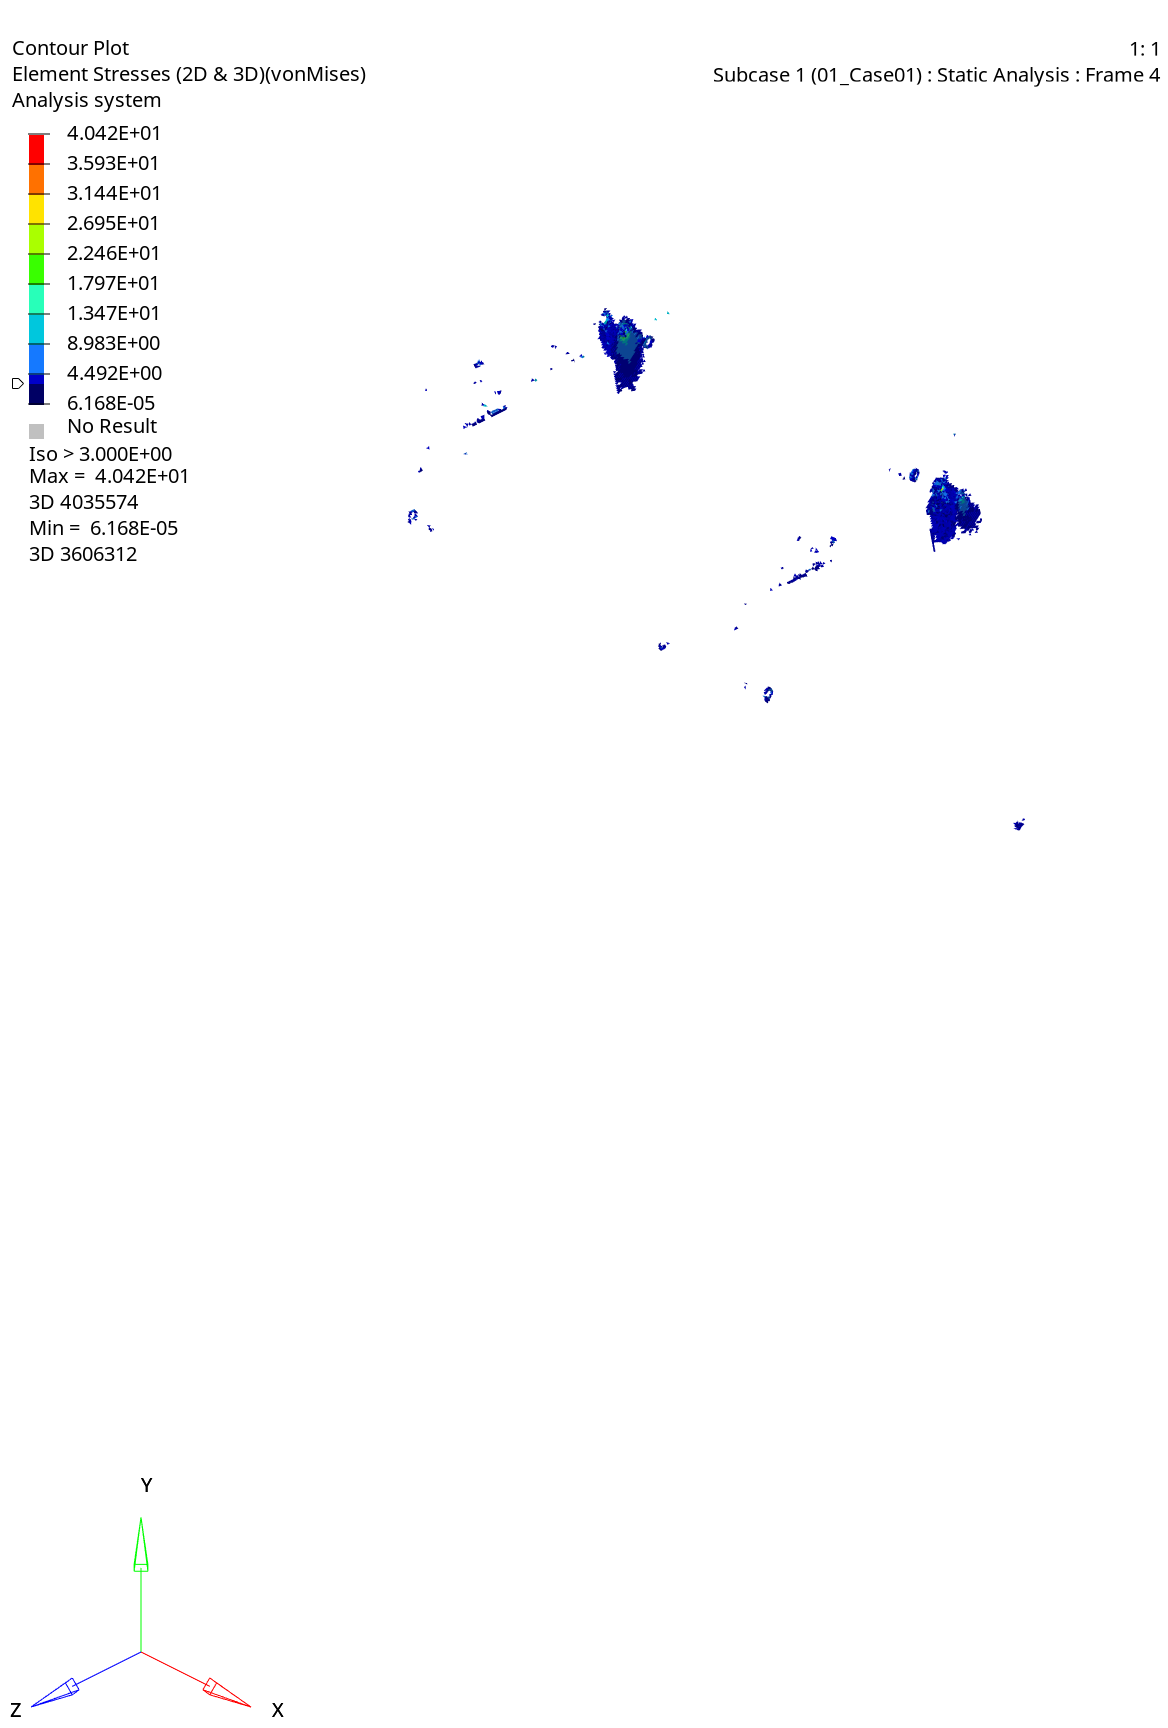
\includegraphics[width=0.48\linewidth]{pics/C010102.png}
    \\
    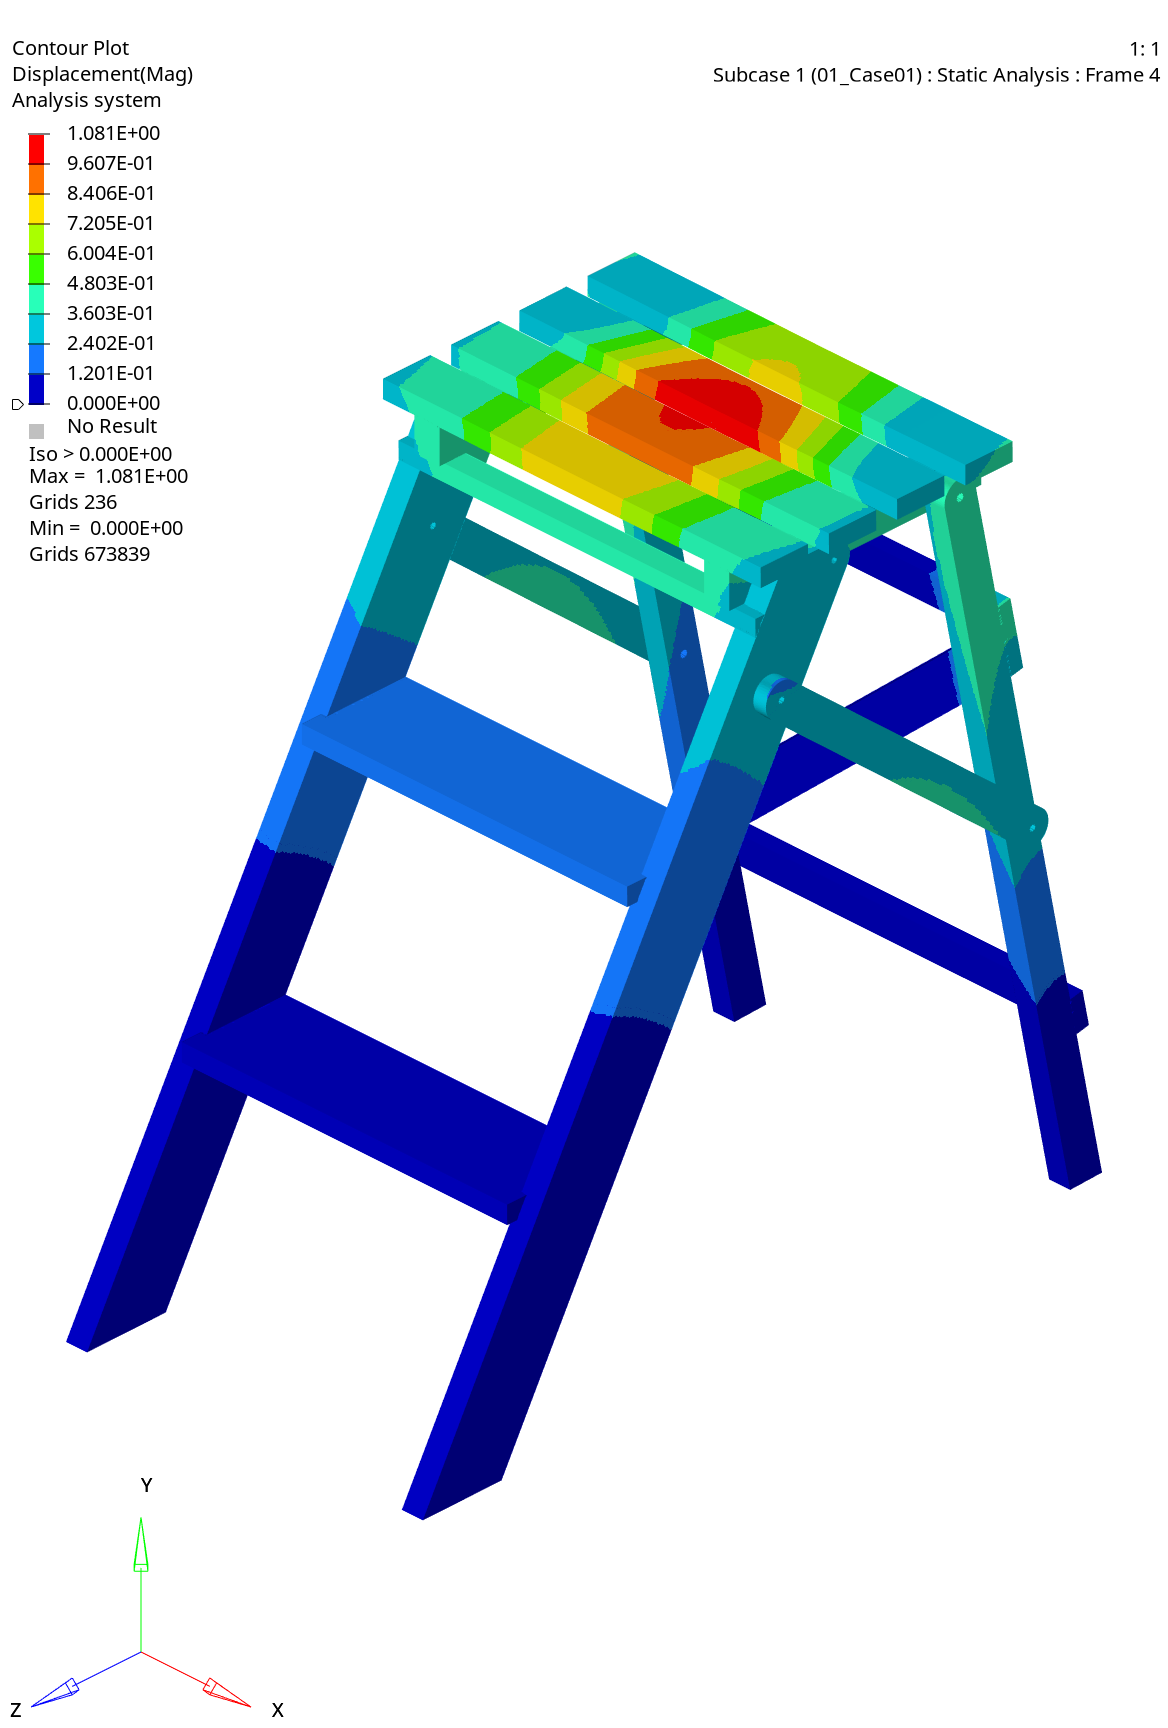
\includegraphics[width=0.48\linewidth]{pics/C010103.png}
    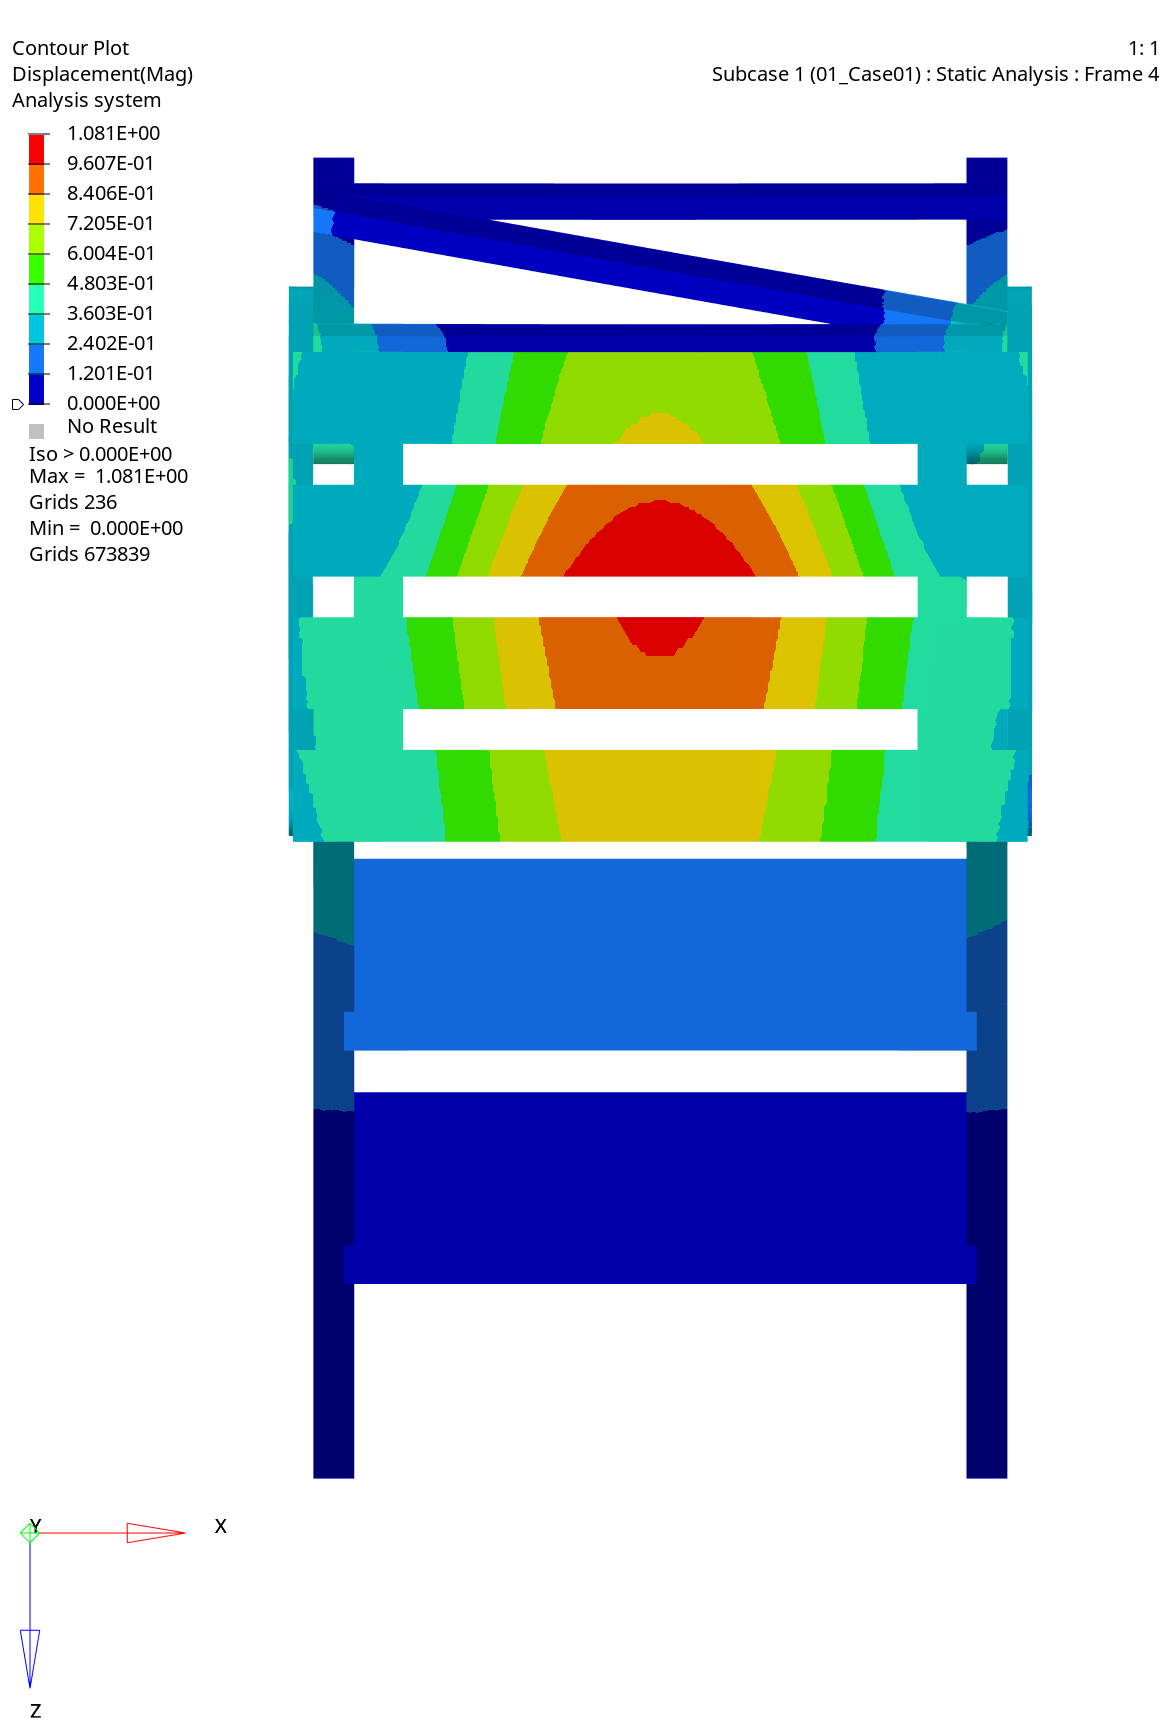
\includegraphics[width=0.48\linewidth]{pics/C010104.png}
    \captionsetup{labelformat=empty}
    \caption{\small{附图1.1: 静态特性分析 - 工况一结果输出}}
    \vspace{-0.4cm}
\end{figure}
\newpage{}
\par{}
\begin{figure}[h]
    \centering
    \vspace{-0.1cm}
    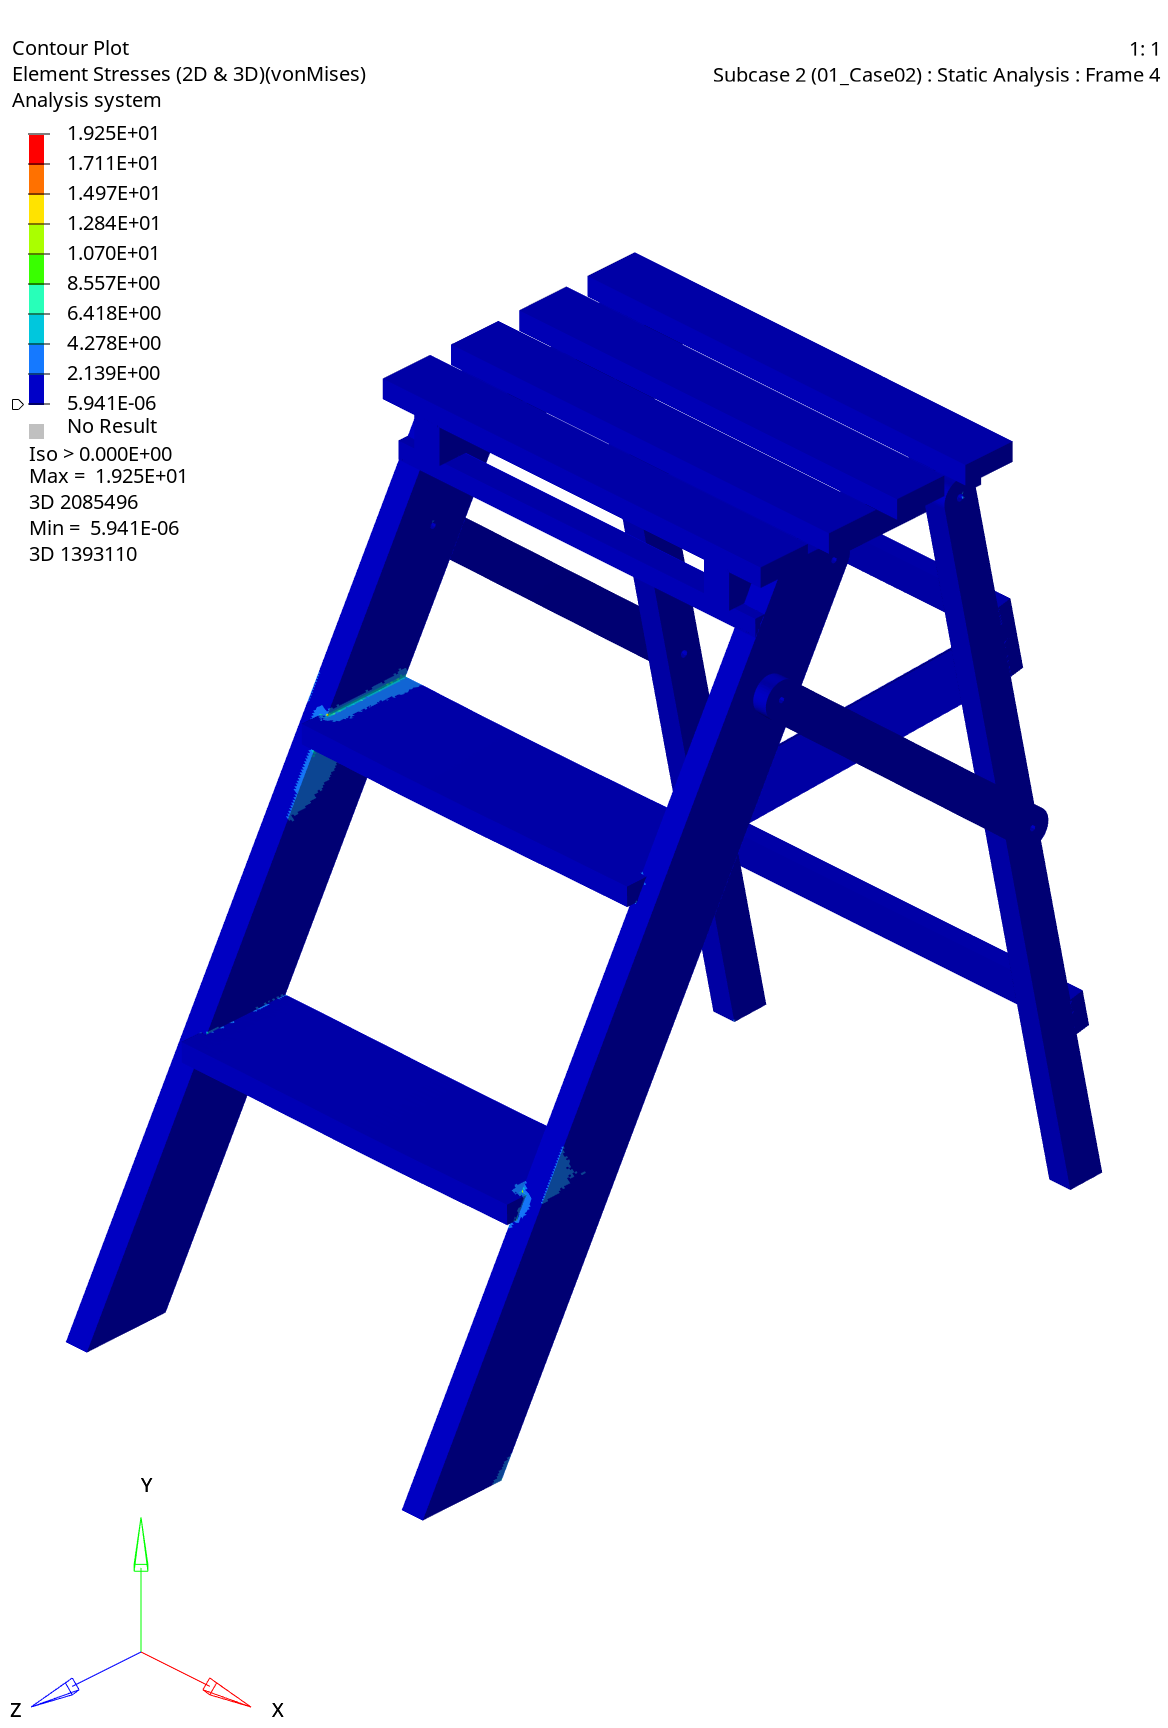
\includegraphics[width=0.48\linewidth]{pics/C010201.png}
    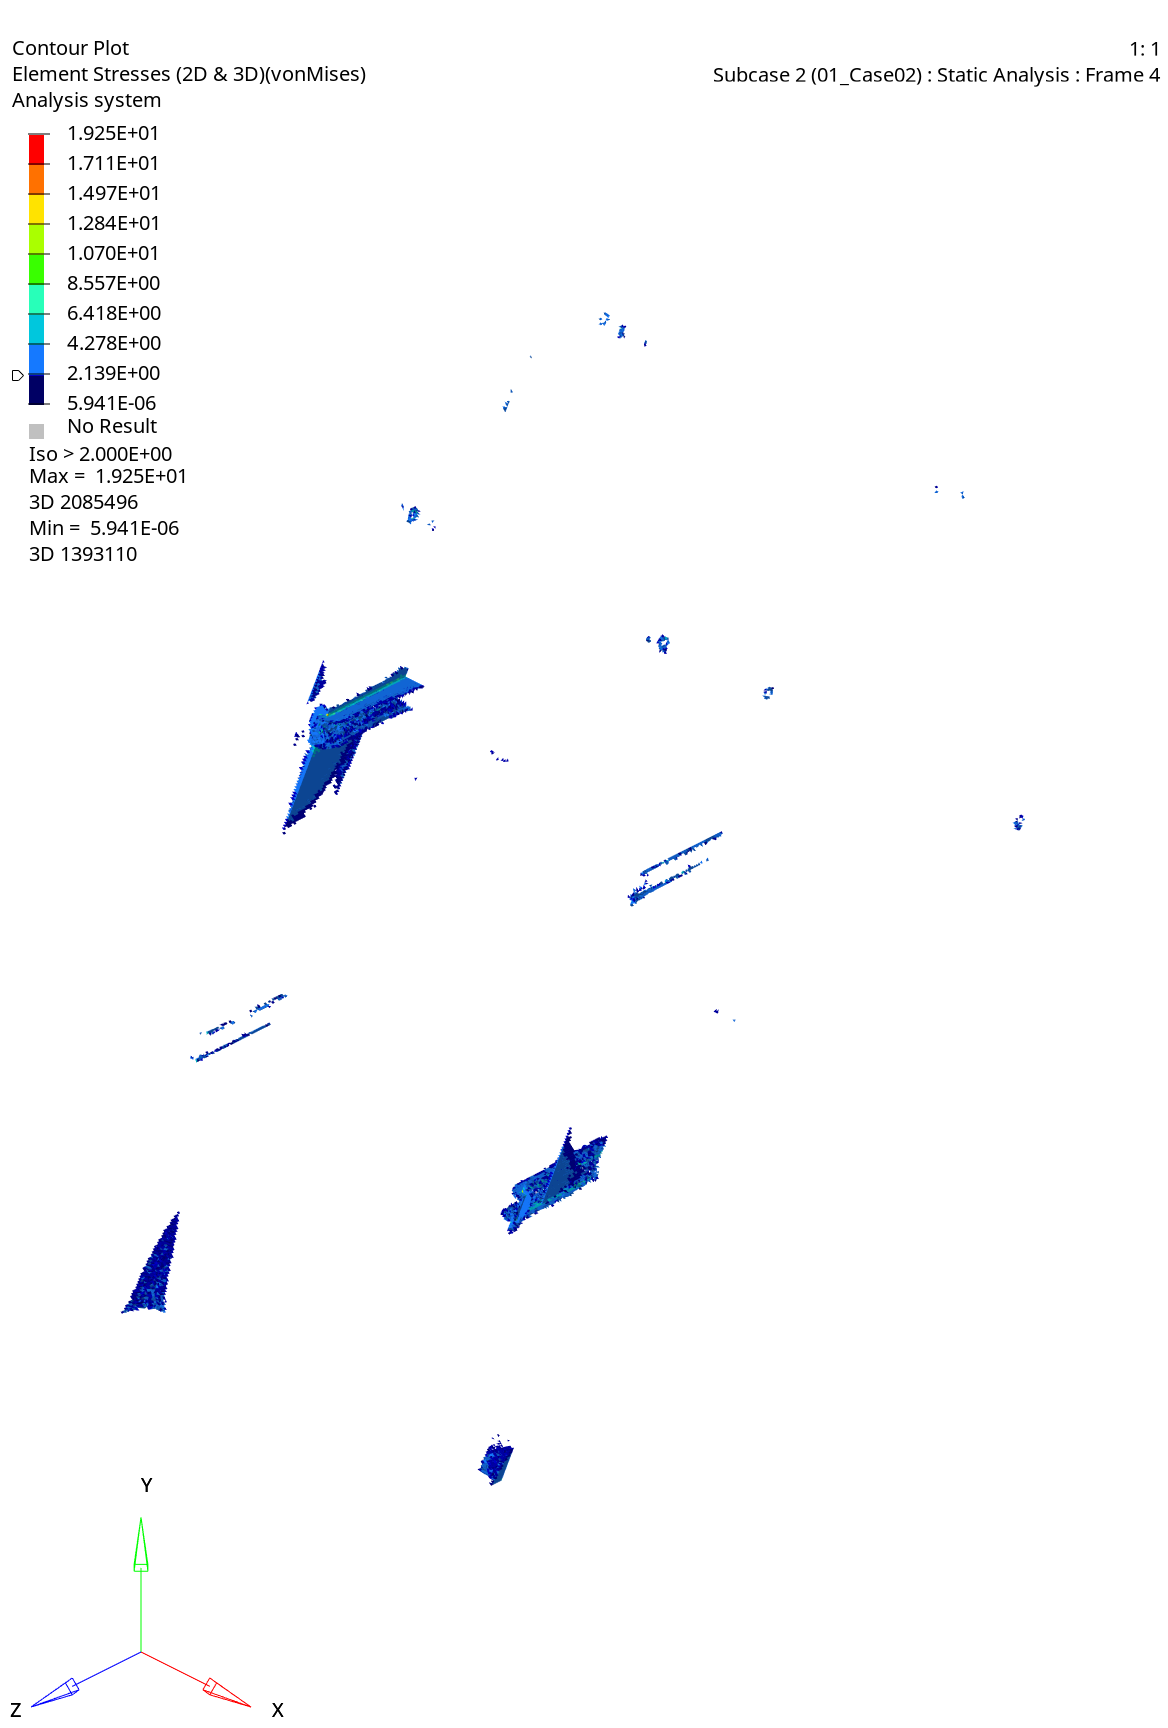
\includegraphics[width=0.48\linewidth]{pics/C010202.png}
    \\
    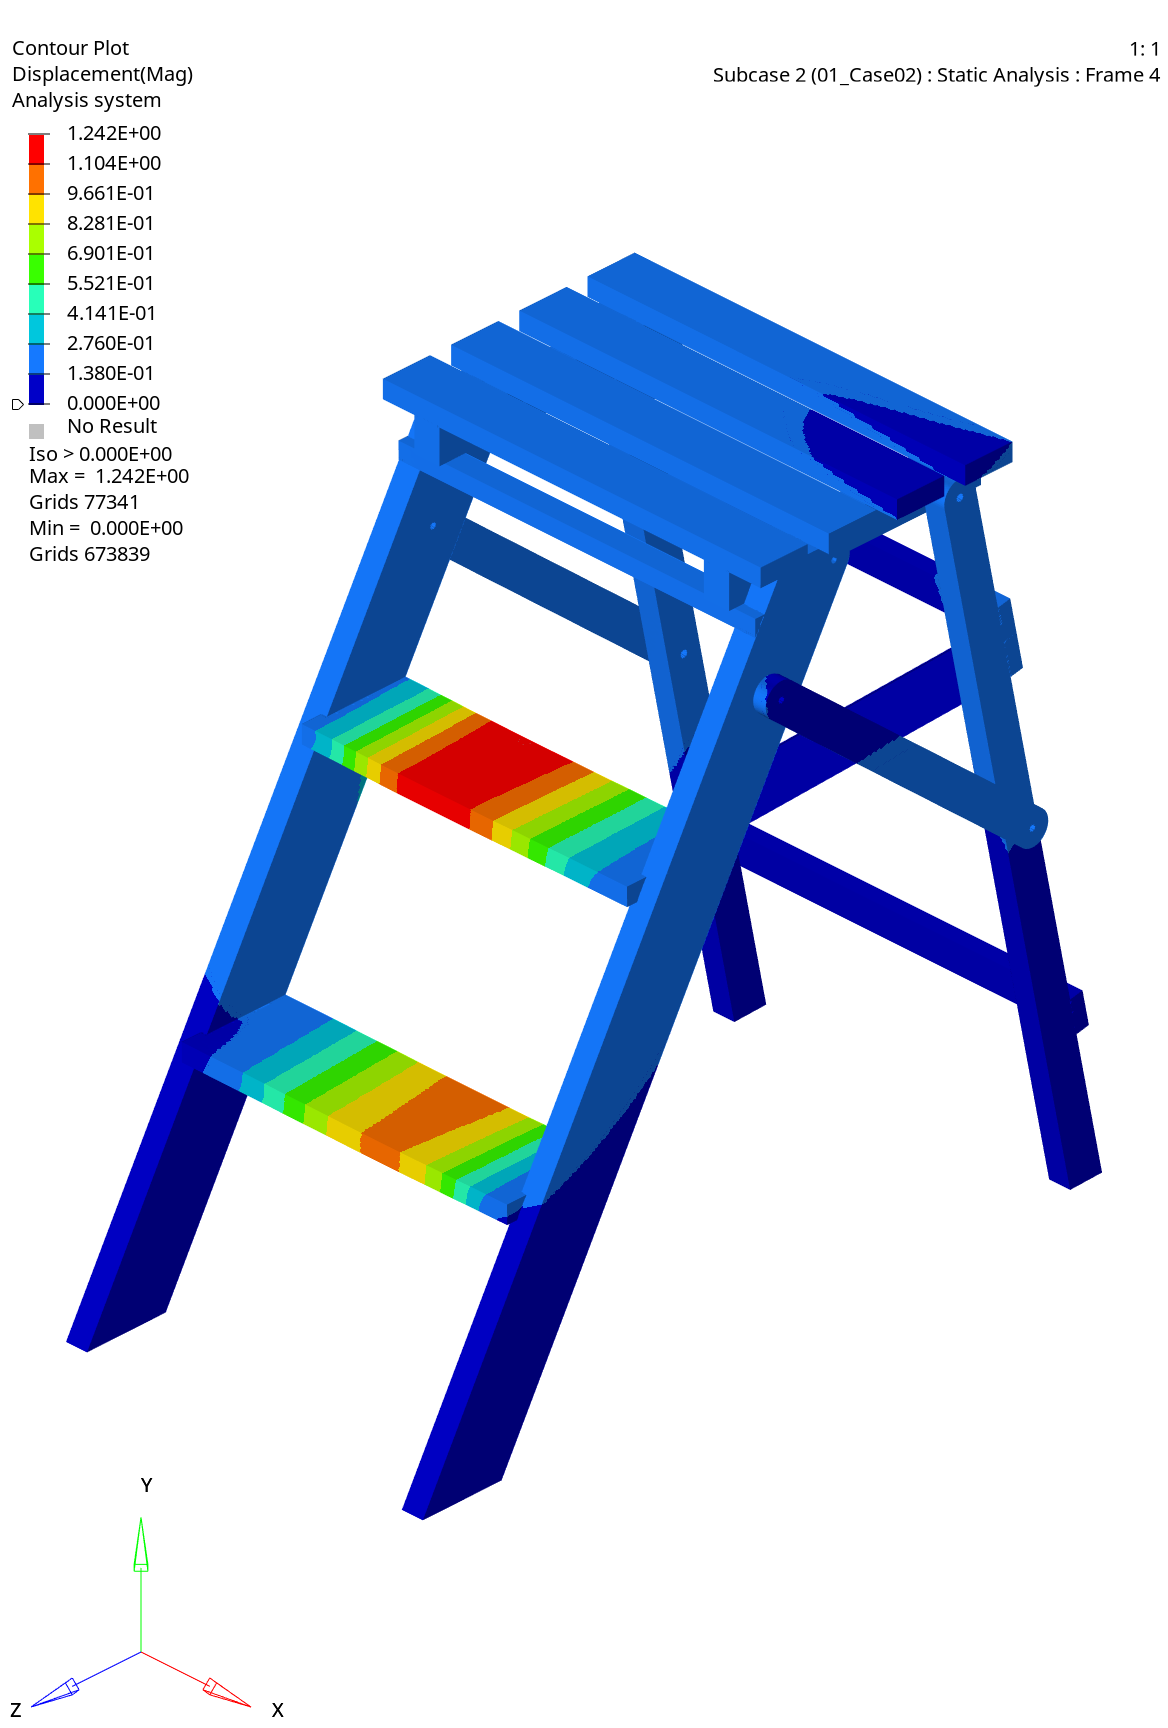
\includegraphics[width=0.48\linewidth]{pics/C010203.png}
    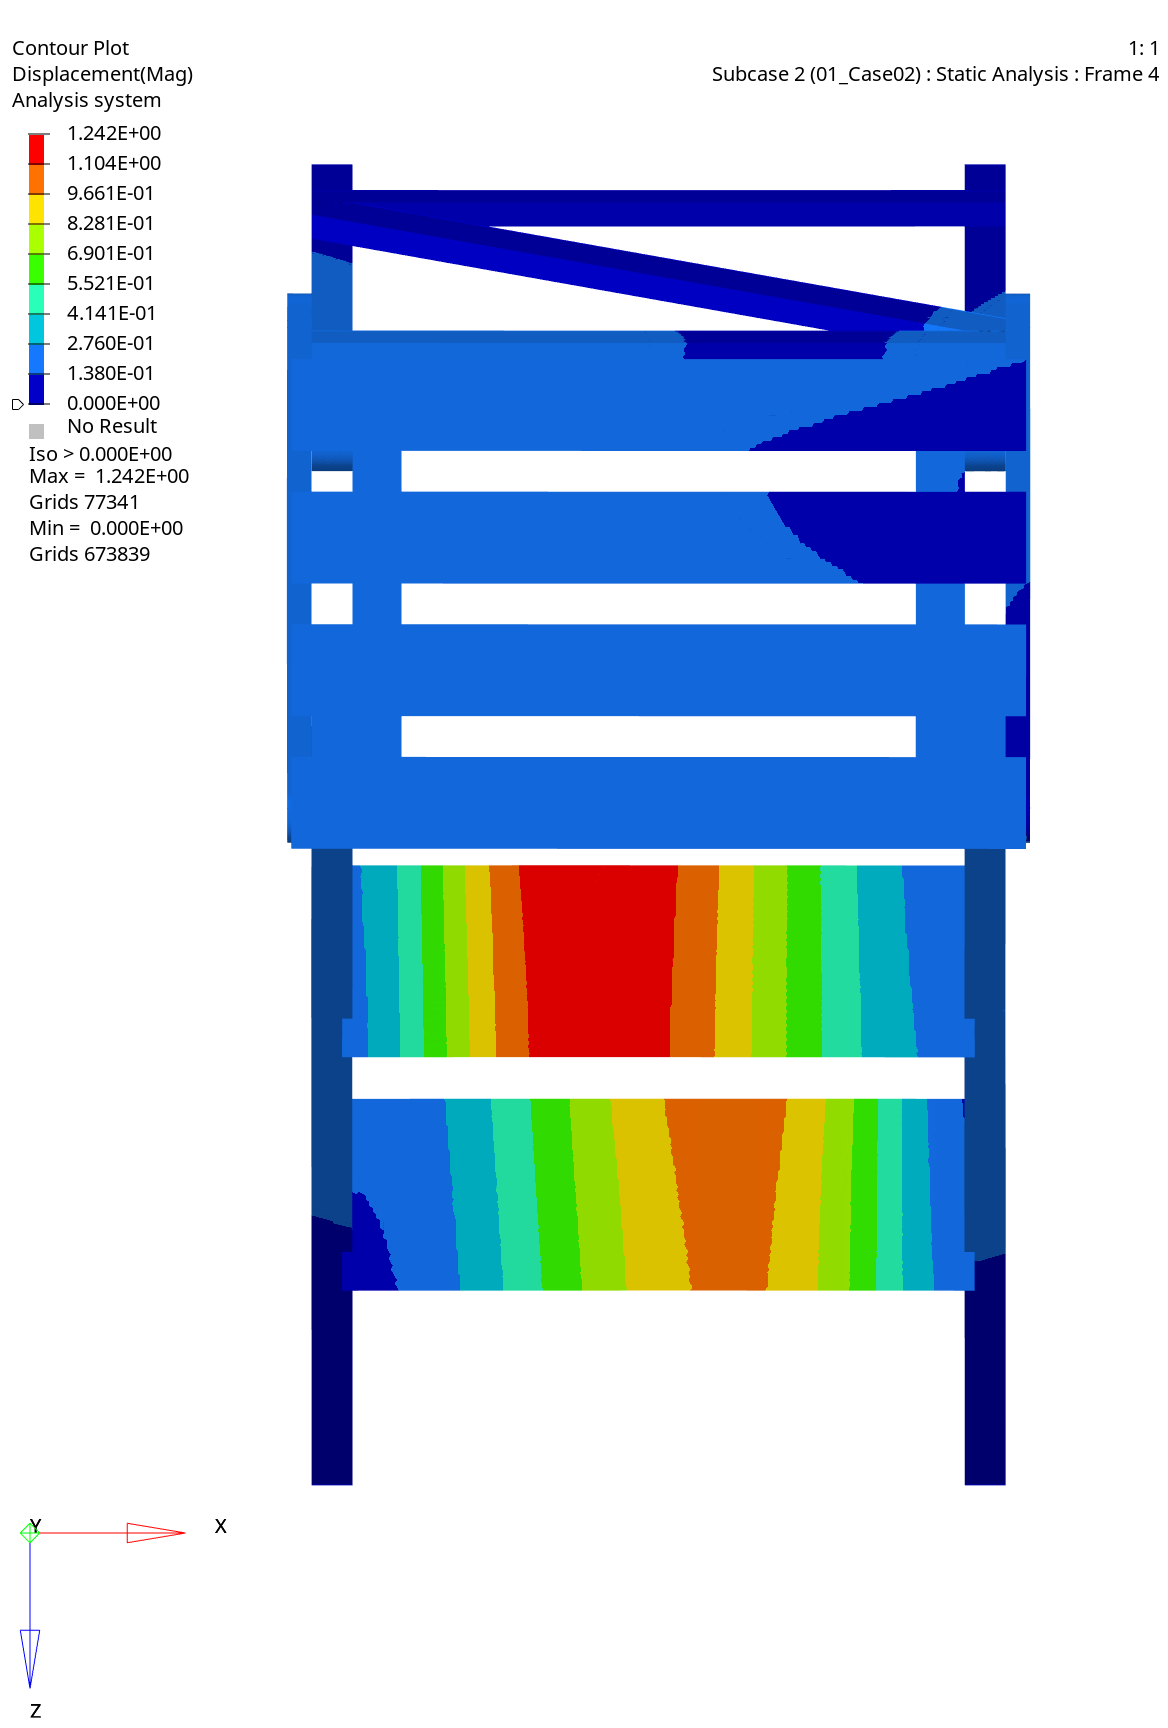
\includegraphics[width=0.48\linewidth]{pics/C010204.png}
    \captionsetup{labelformat=empty}
    \caption{\small{附图1.2: 静态特性分析 - 工况二结果输出}}
    \vspace{-0.4cm}
\end{figure}
\newpage{}
\par{}
\begin{figure}[h]
    \centering
    \vspace{-0.1cm}
    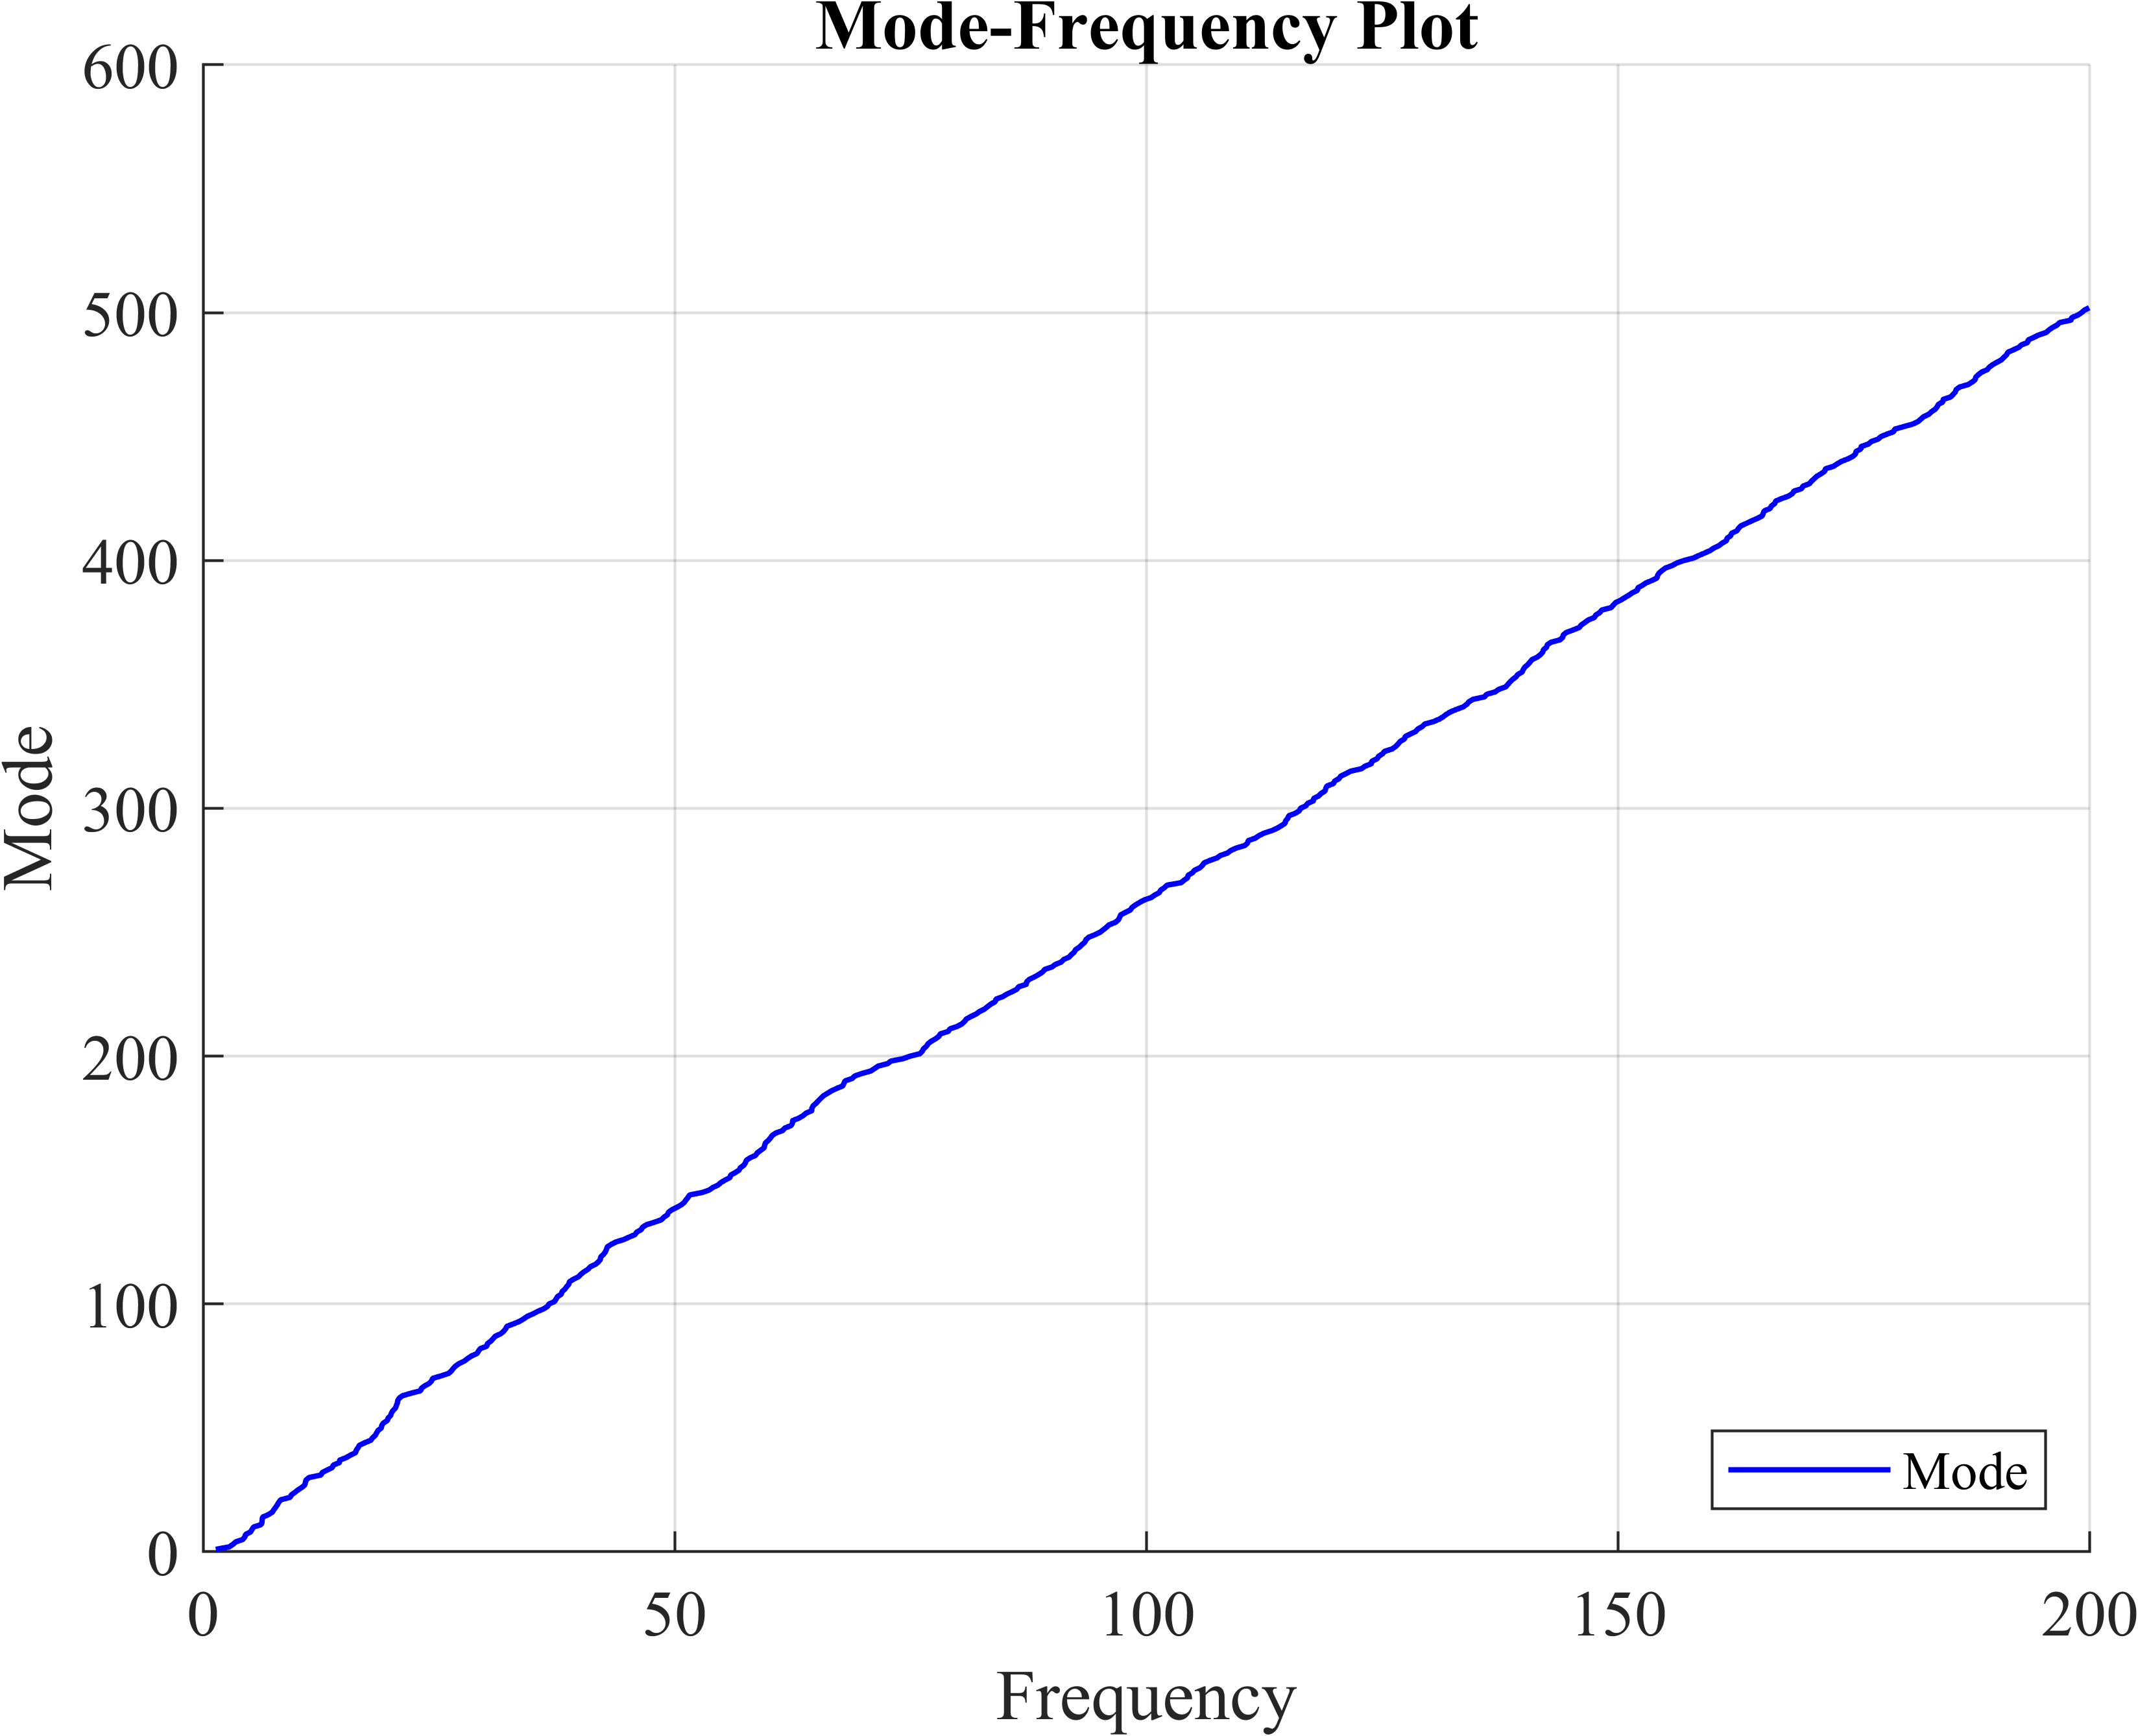
\includegraphics[width=0.6\linewidth]{pics/C020101.png}
    \\
    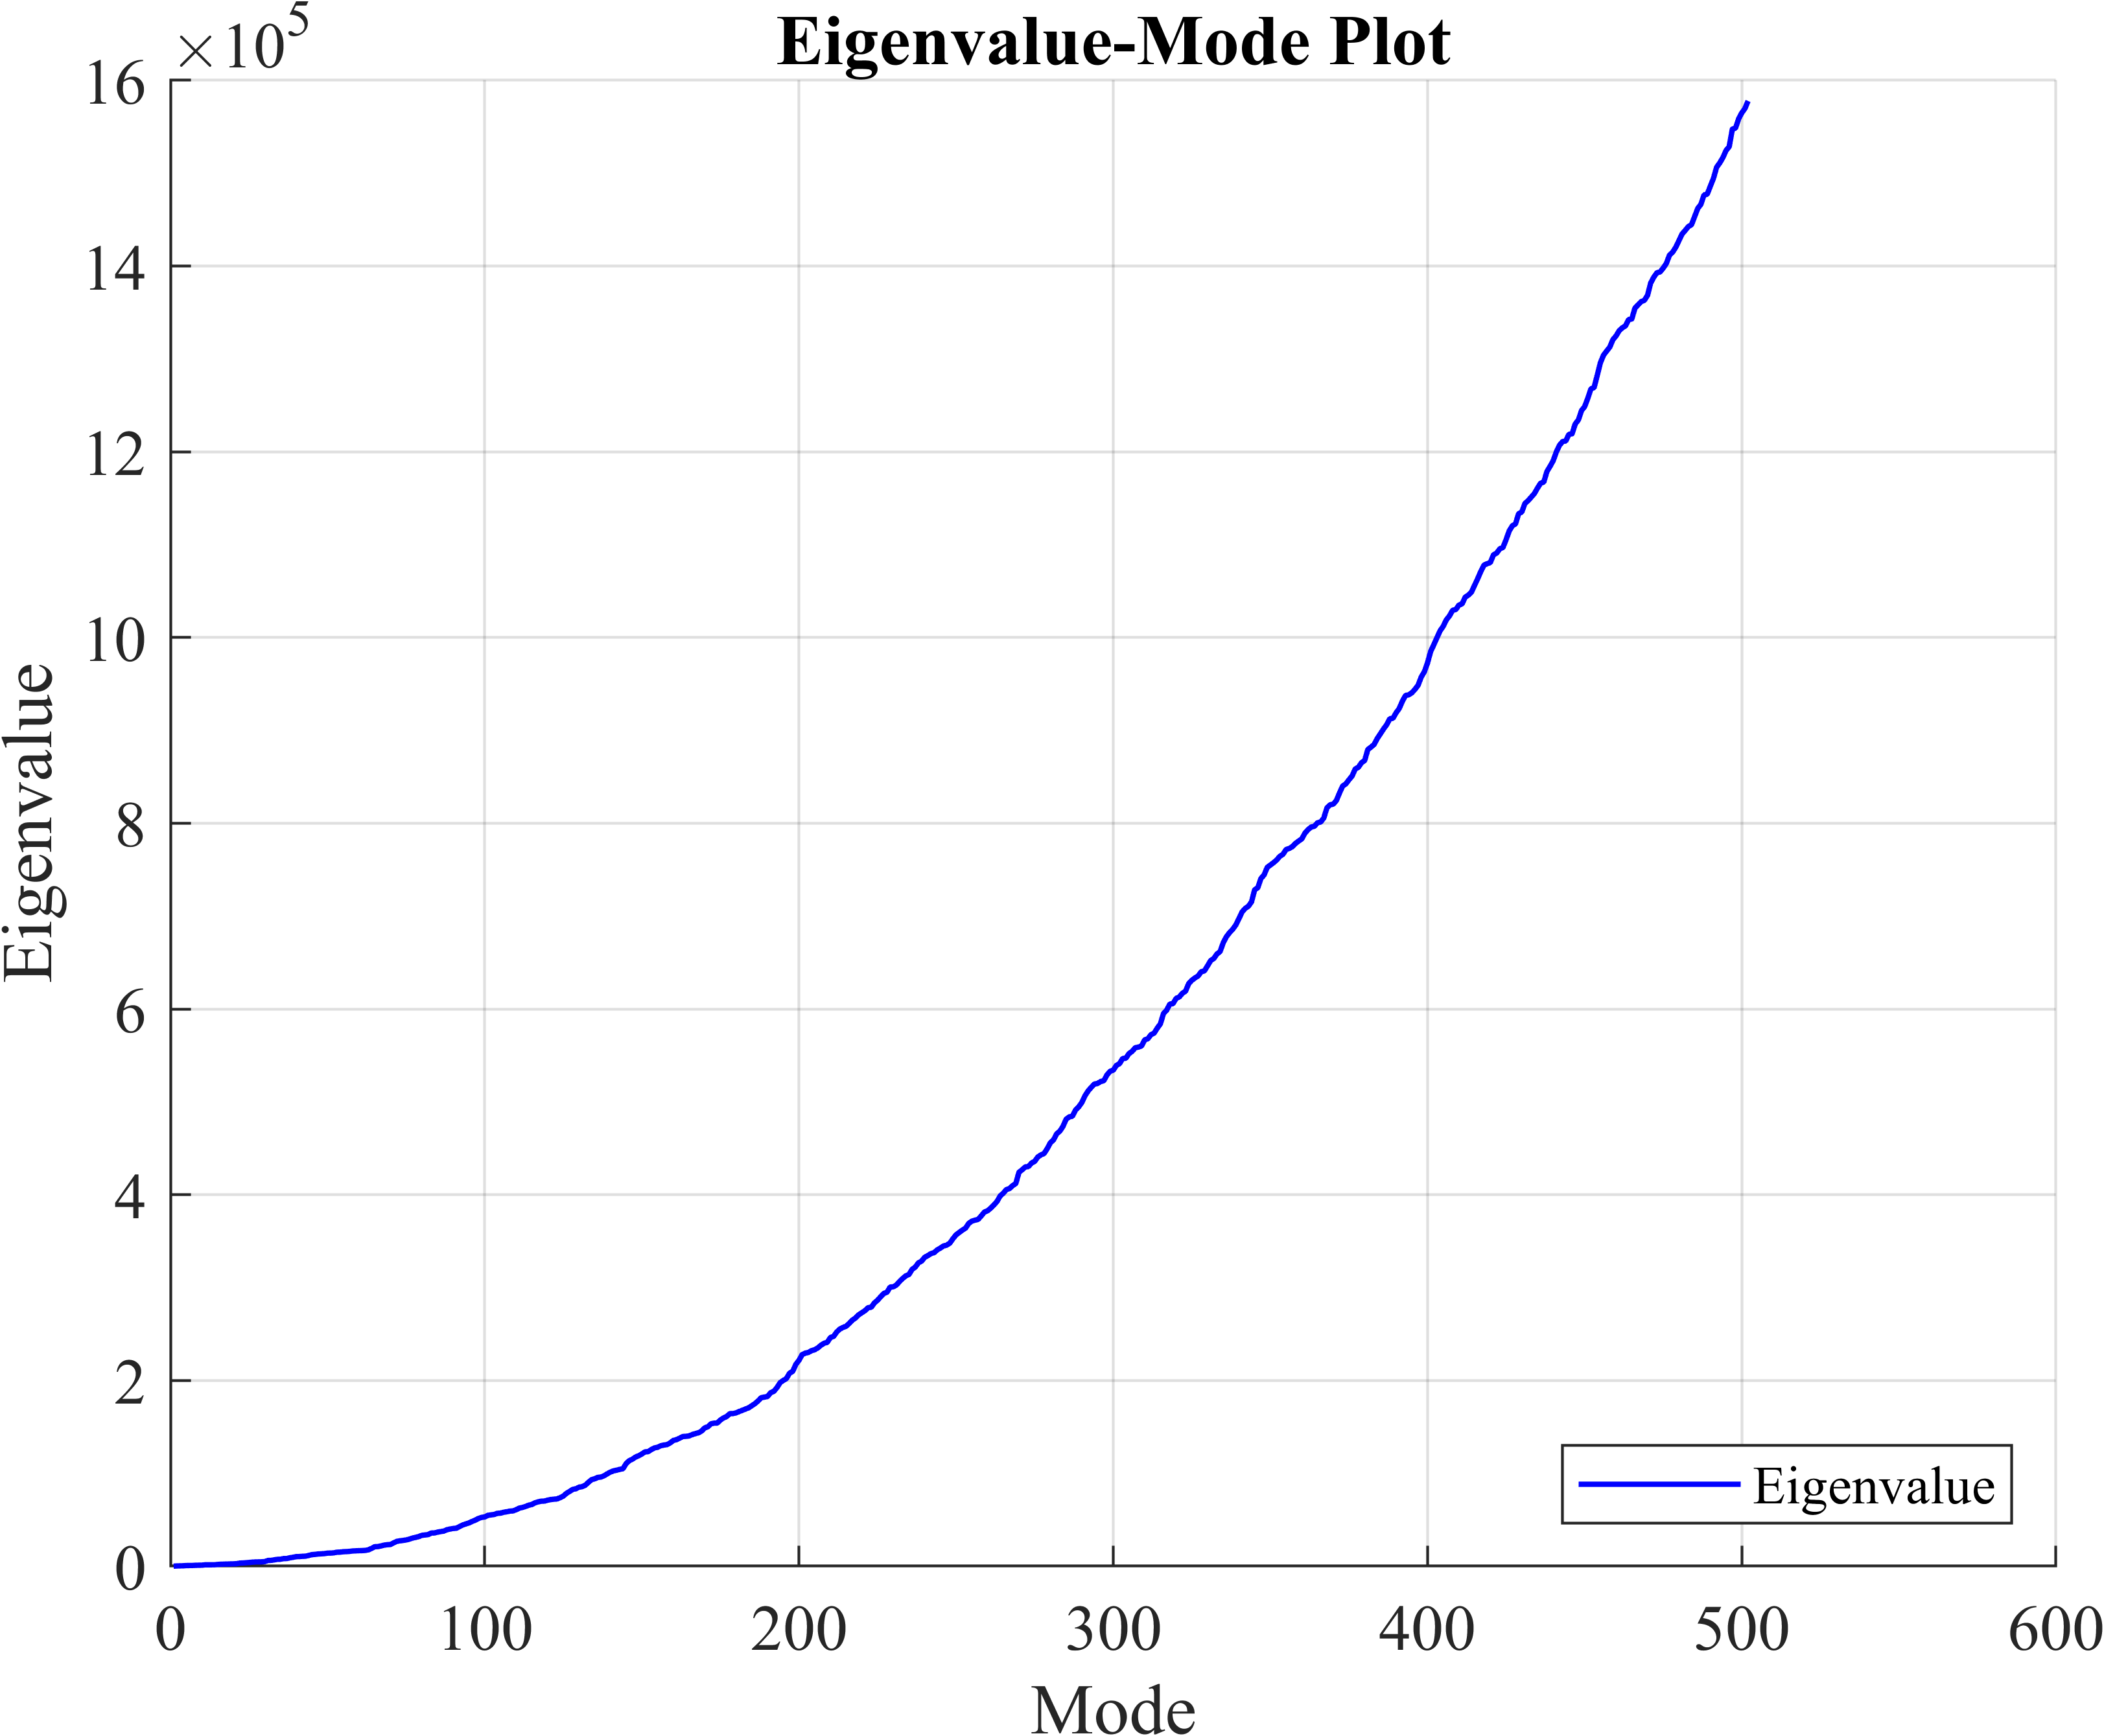
\includegraphics[width=0.6\linewidth]{pics/C020102.png}
    \\
    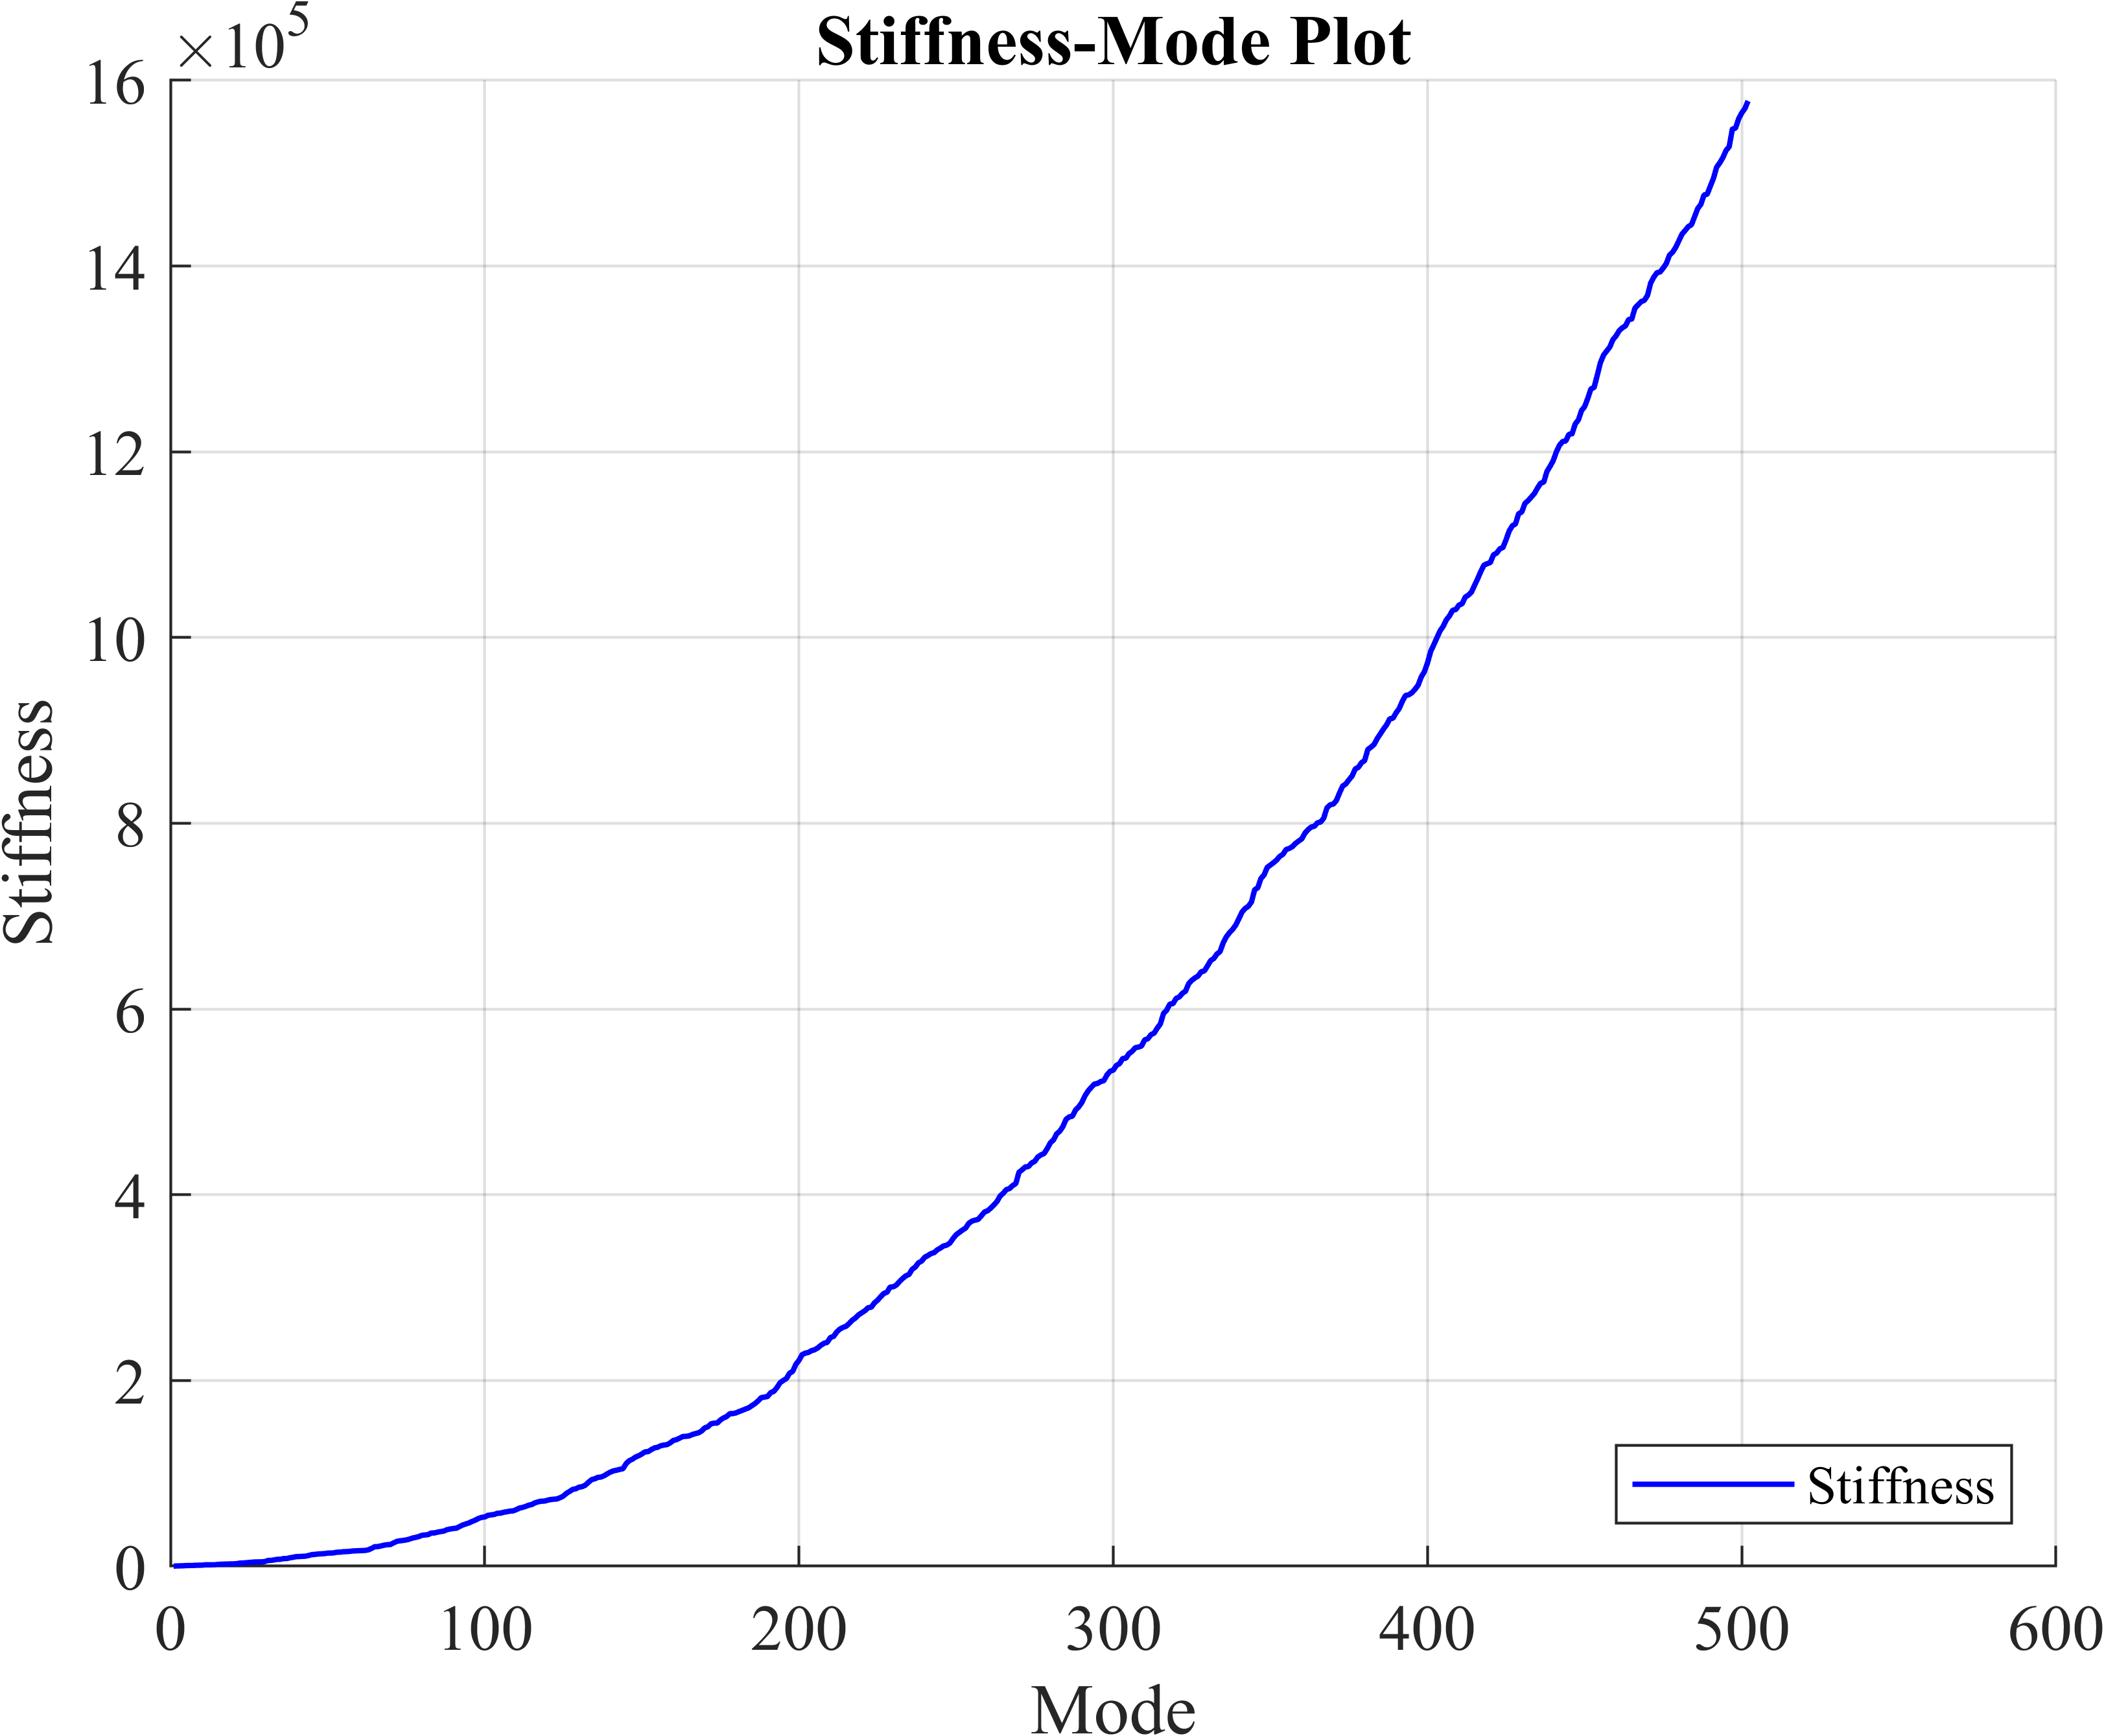
\includegraphics[width=0.6\linewidth]{pics/C020103.png}
    \captionsetup{labelformat=empty}
    \caption{\small{附图2.1: 动态特性分析 - 模态分析结果概览}}
    \vspace{-0.4cm}
\end{figure}
\newpage{}
\par{}
\begin{figure}[h]
    \centering
    \vspace{-0.1cm}
    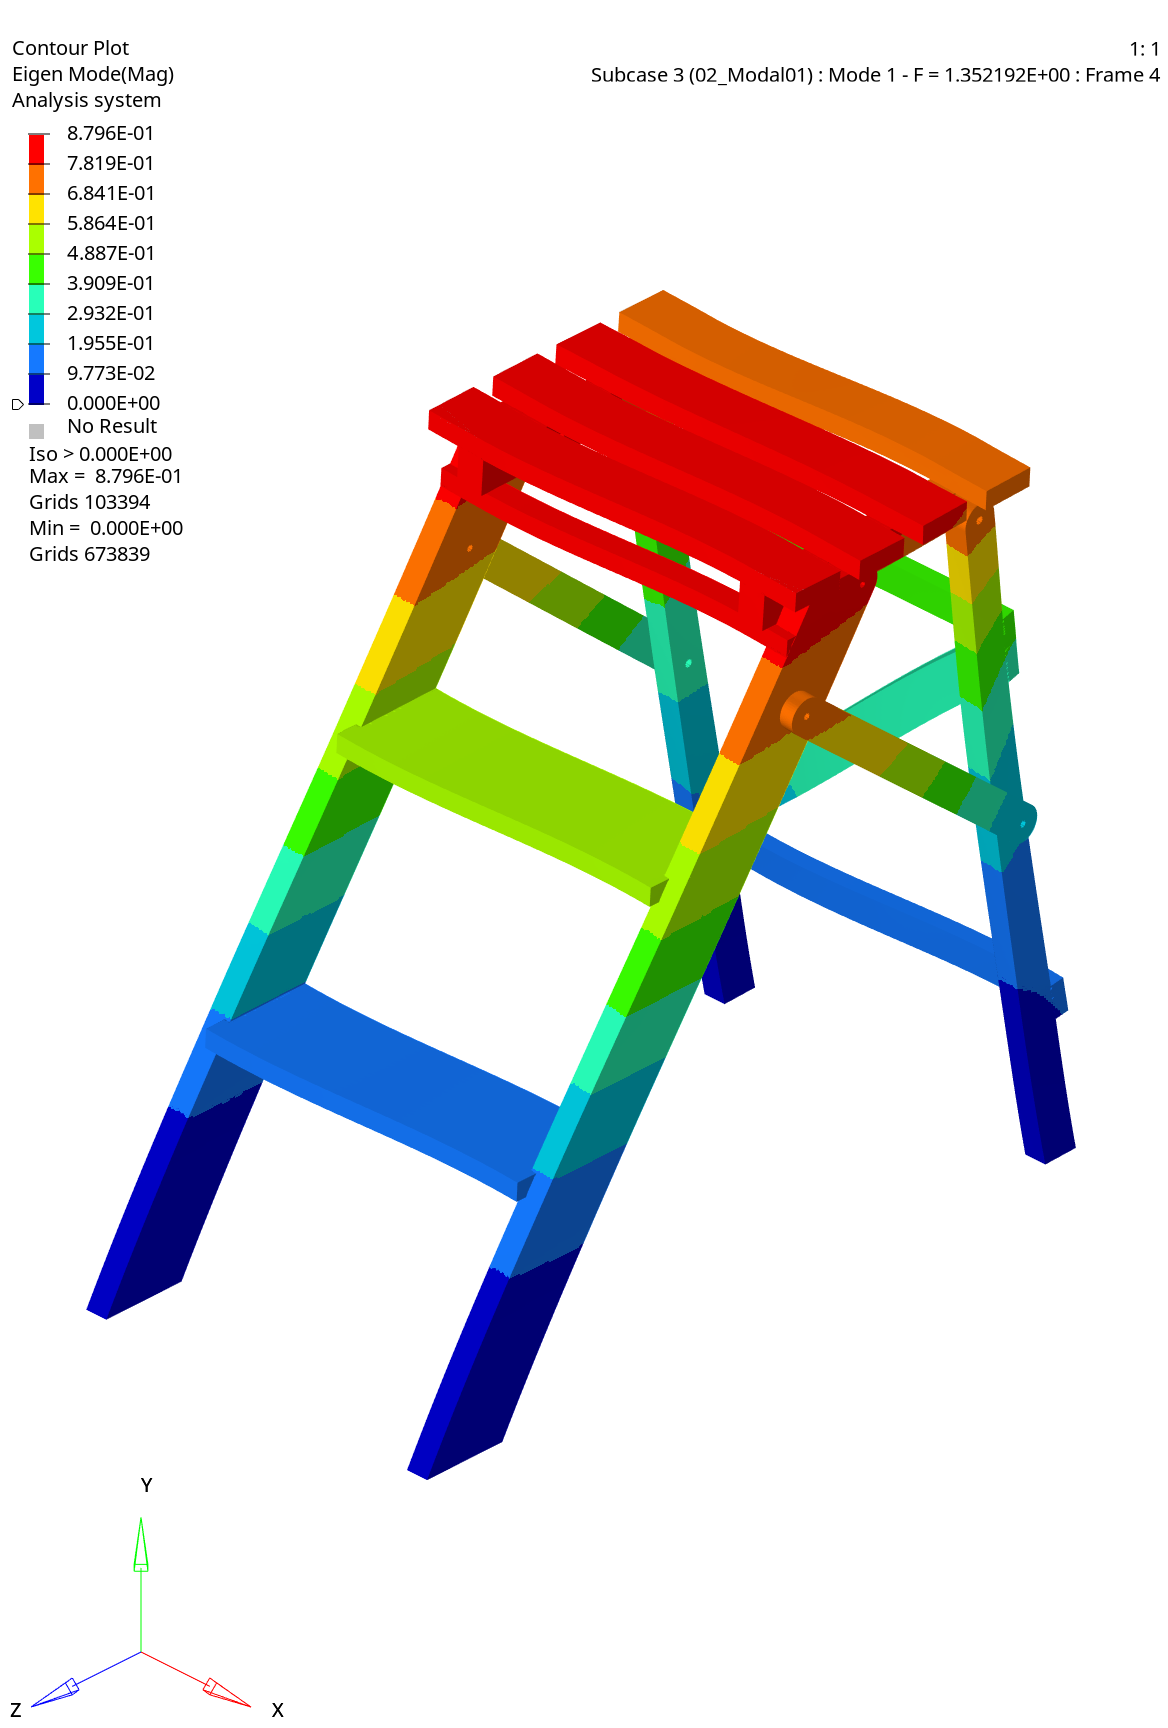
\includegraphics[width=0.32\linewidth]{pics/C020201_001.png}
    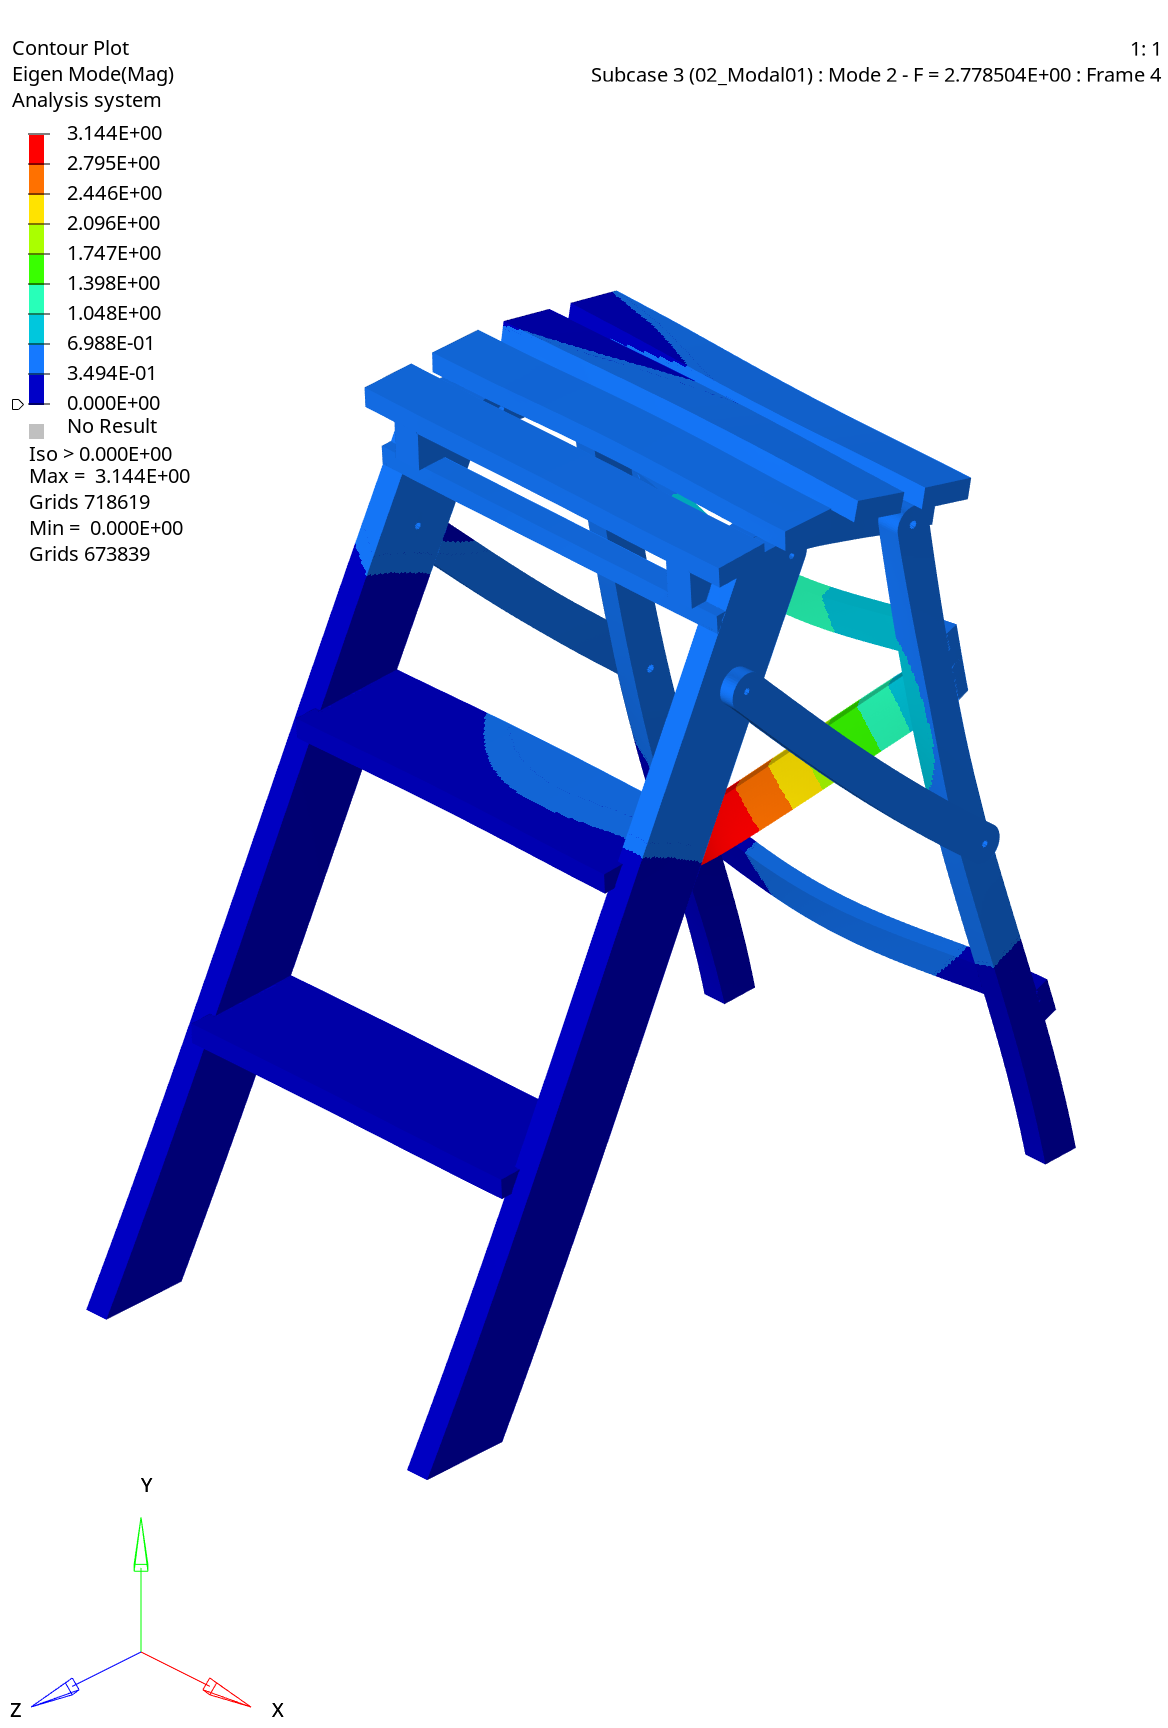
\includegraphics[width=0.32\linewidth]{pics/C020202_002.png}
    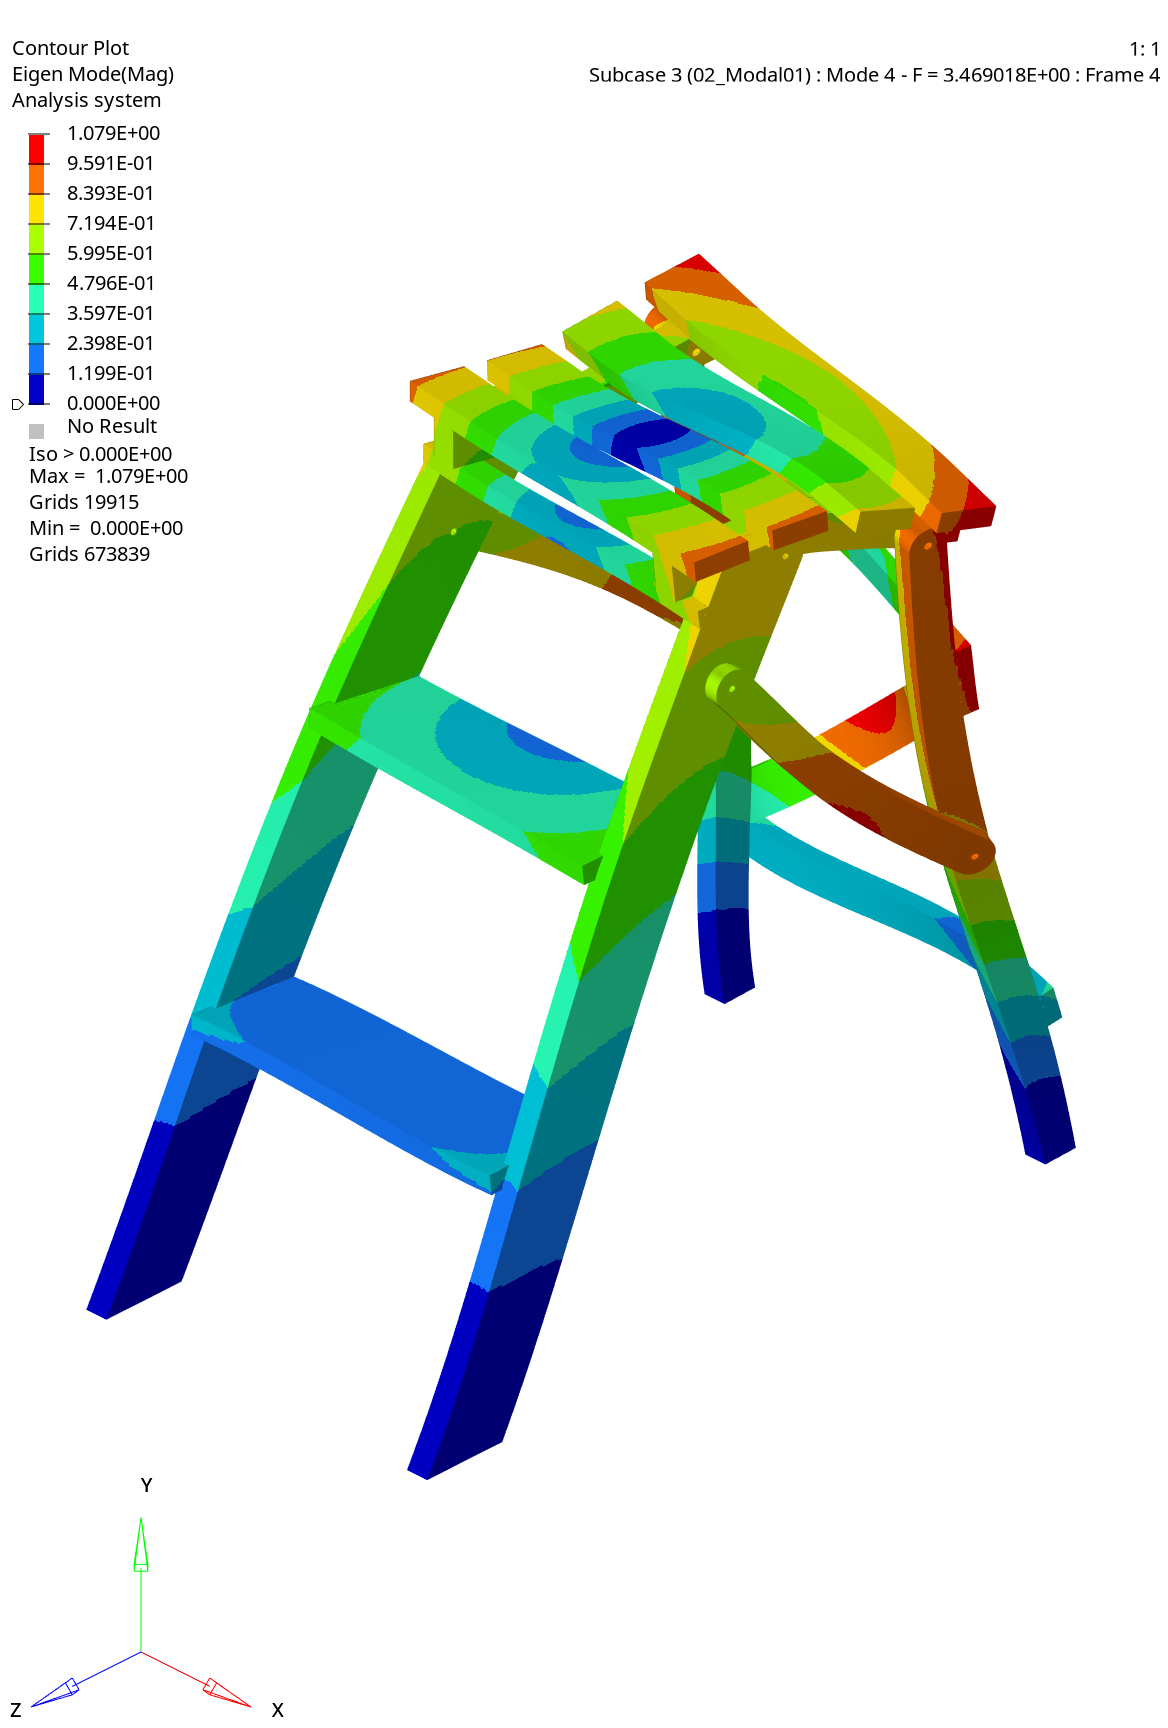
\includegraphics[width=0.32\linewidth]{pics/C020203_004.png}
    \\
    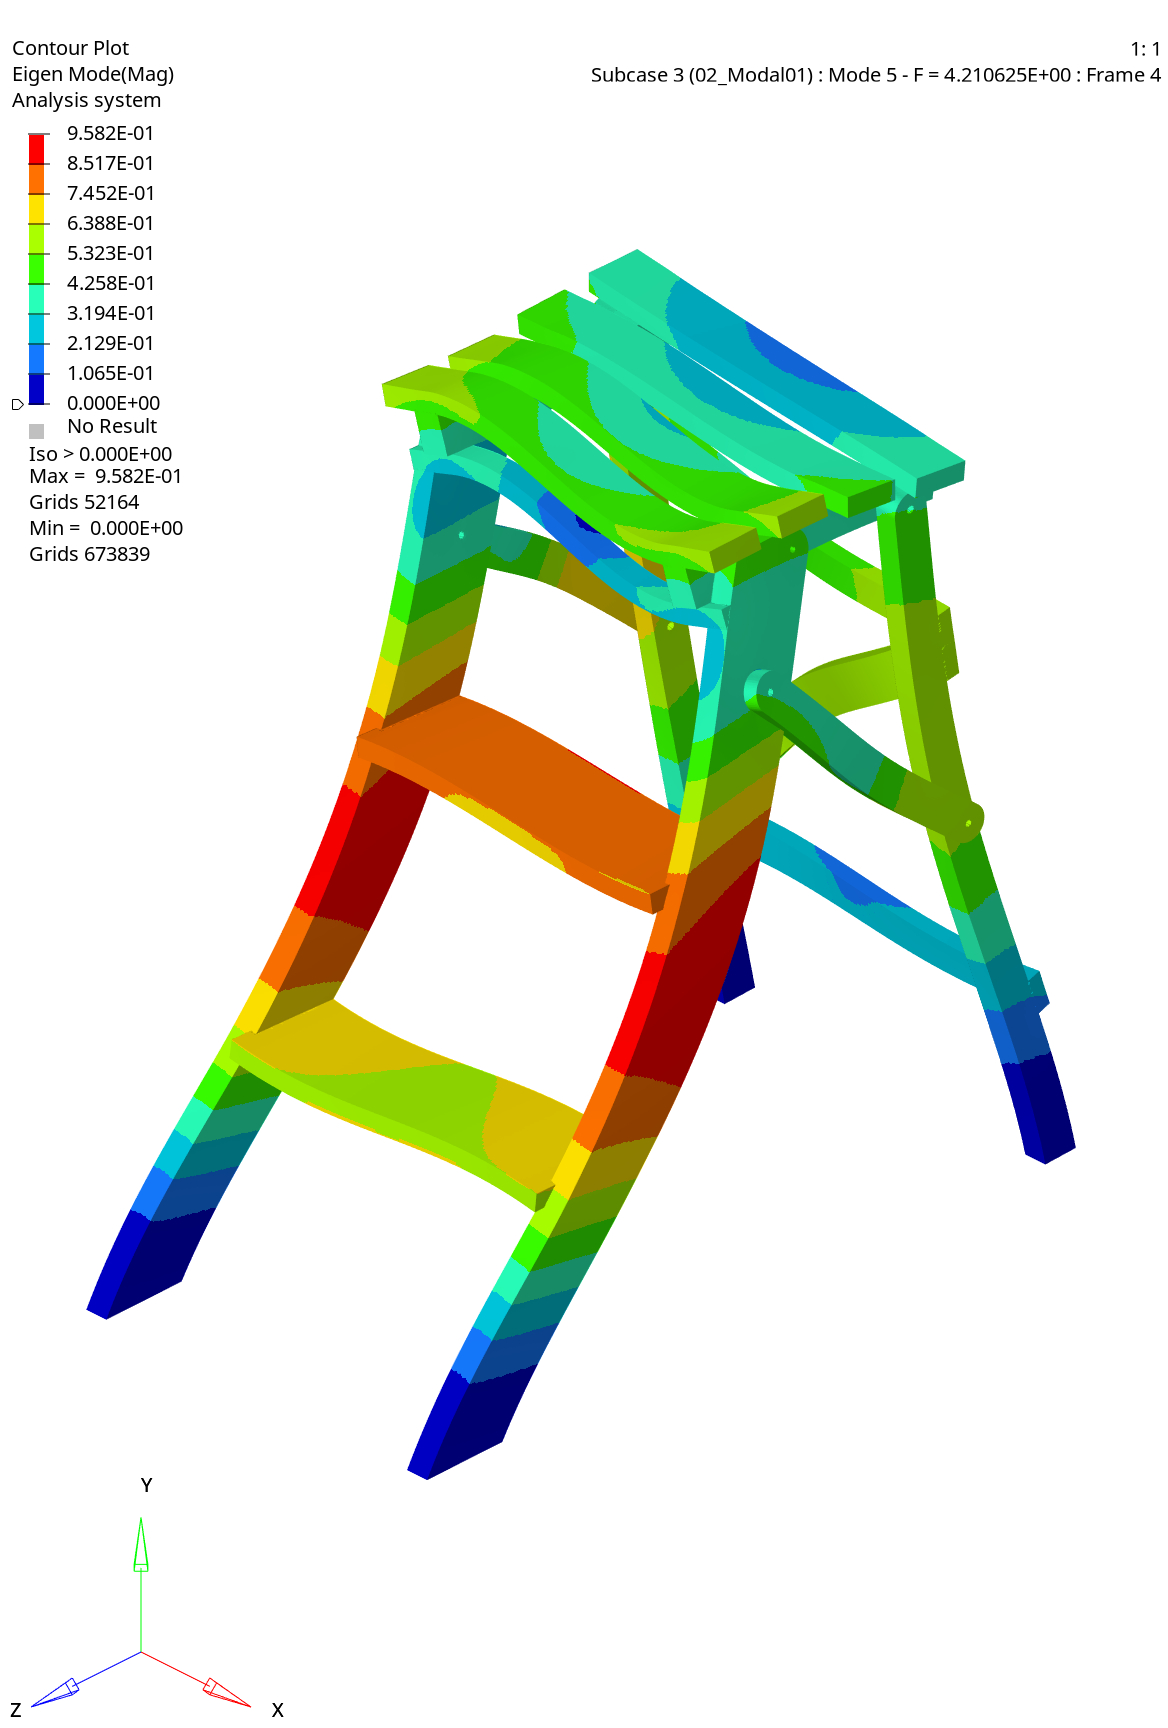
\includegraphics[width=0.32\linewidth]{pics/C020204_005.png}
    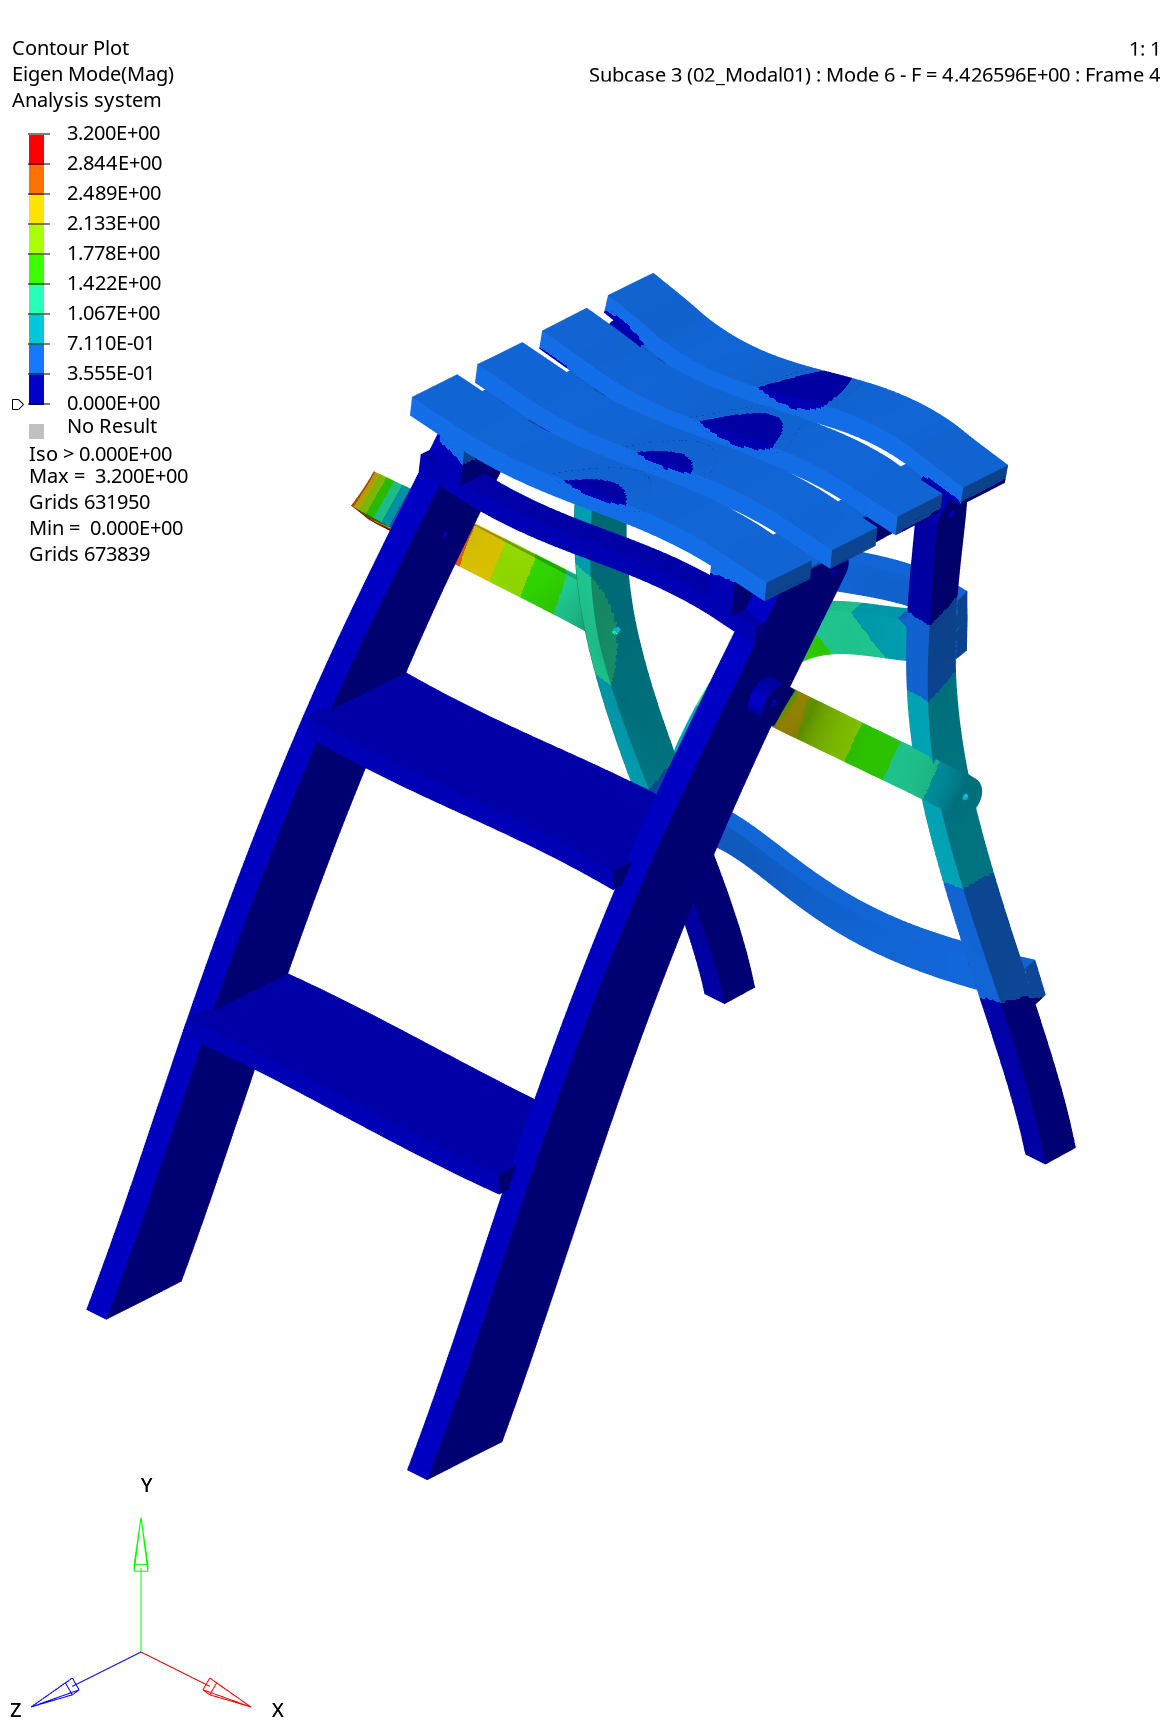
\includegraphics[width=0.32\linewidth]{pics/C020205_006.png}
    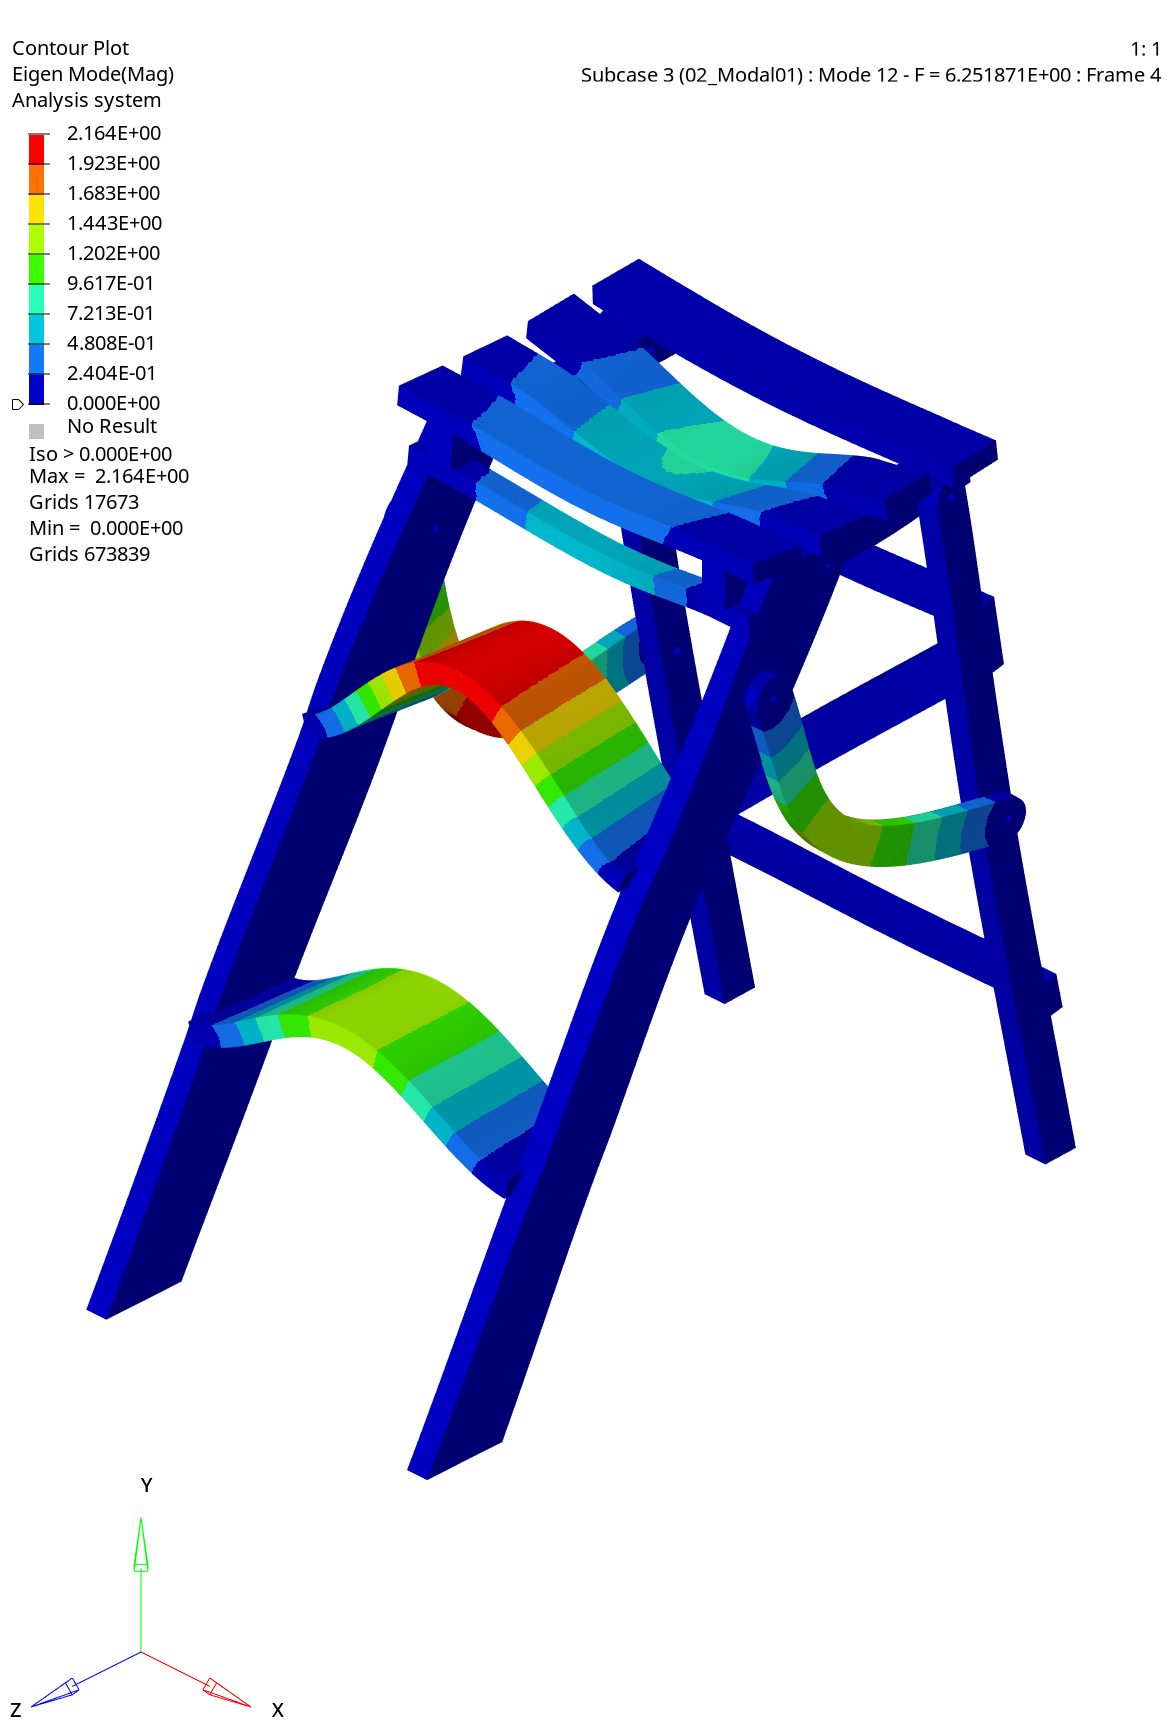
\includegraphics[width=0.32\linewidth]{pics/C020206_012.png}
    \captionsetup{labelformat=empty}
    \caption{\small{附图2.2: 动态特性分析 - 模态分析代表性结果输出}}
    \vspace{-0.4cm}
\end{figure}
\newpage{}
\par{}
\begin{figure}[h]
    \centering
    \vspace{-0.1cm}
    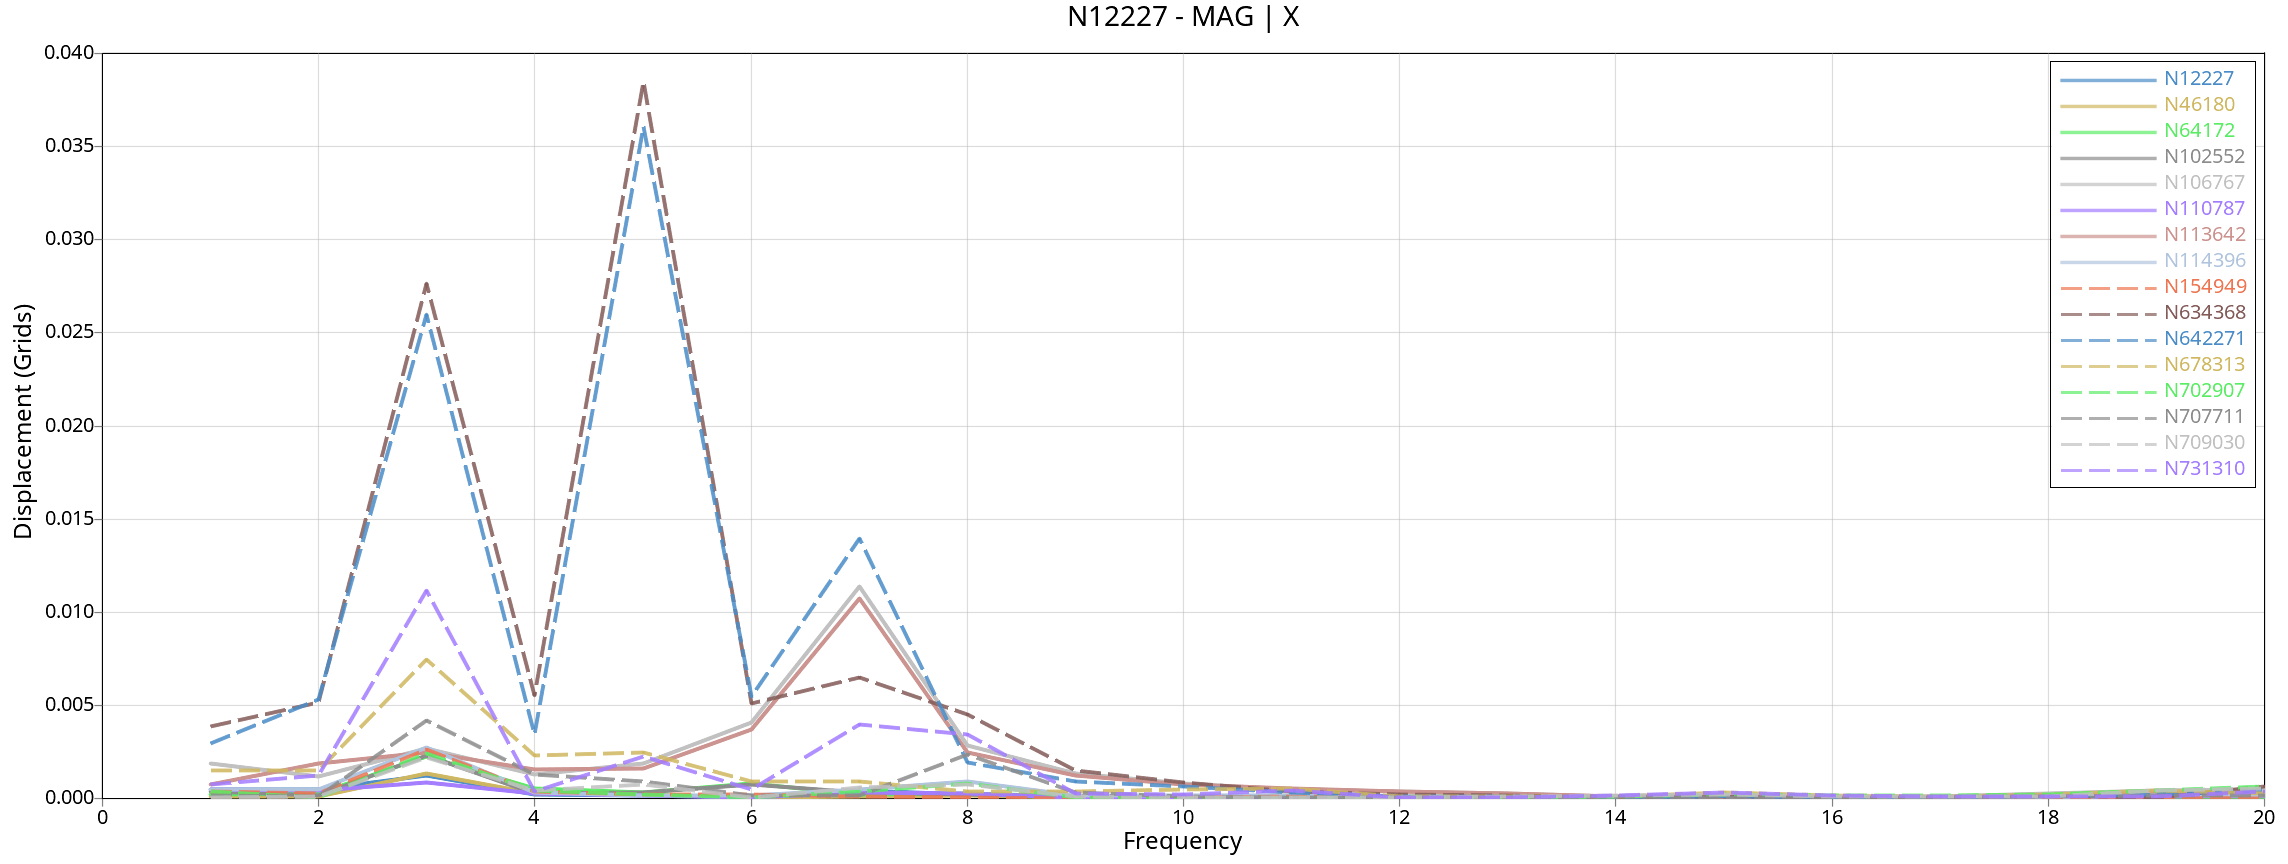
\includegraphics[width=0.7\linewidth]{pics/C020301_dx.png}
    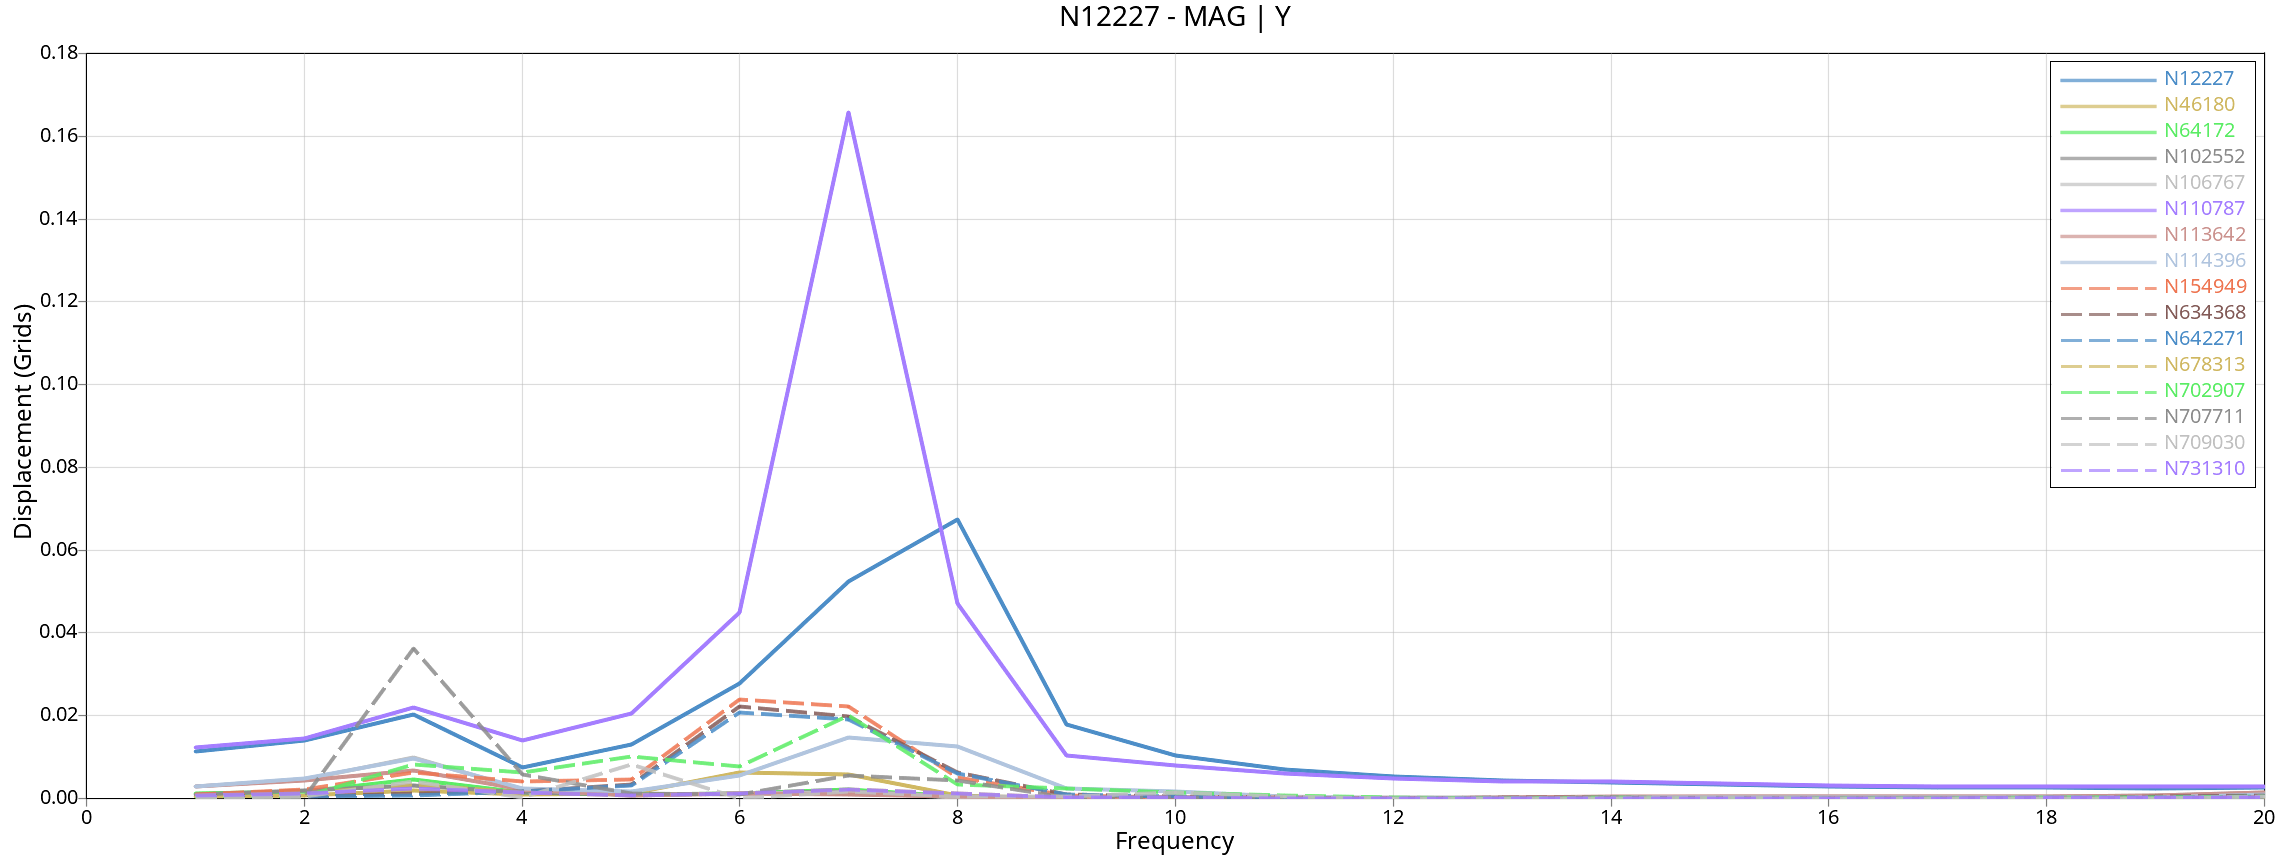
\includegraphics[width=0.7\linewidth]{pics/C020302_dy.png}
    \\
    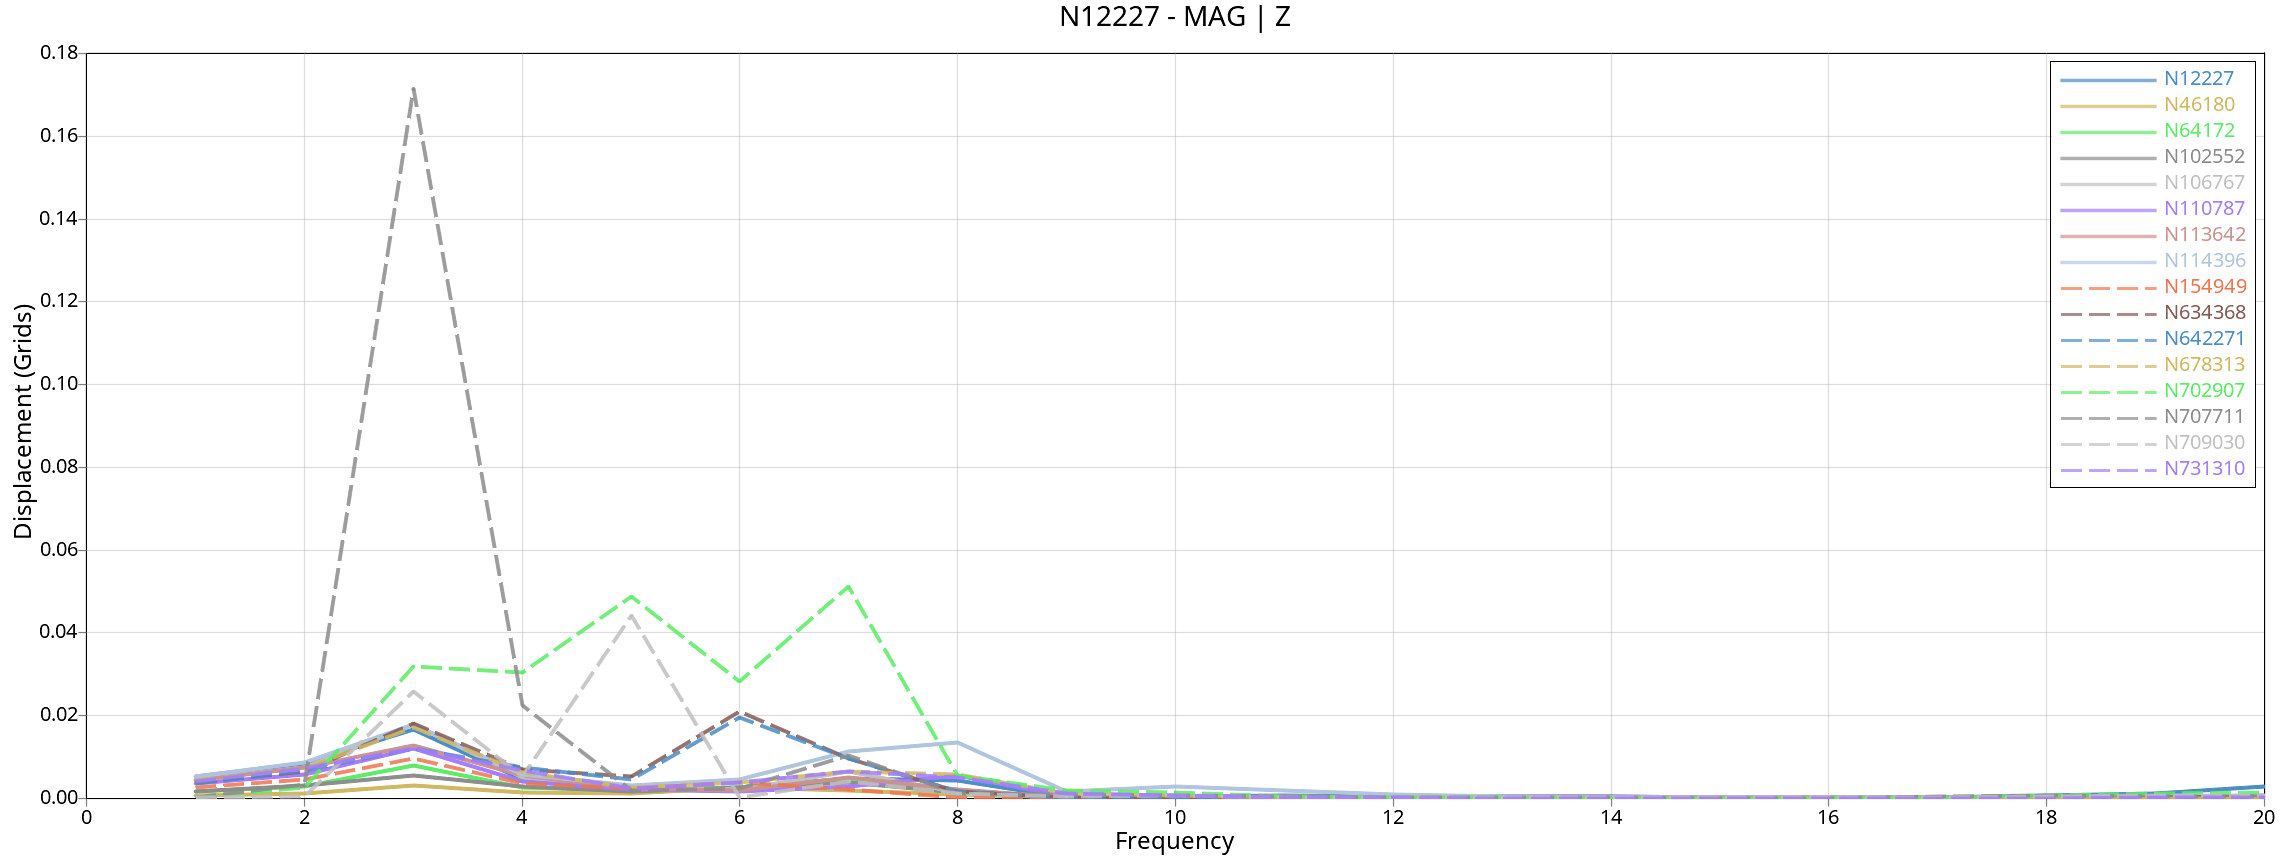
\includegraphics[width=0.7\linewidth]{pics/C020303_dz.png}
    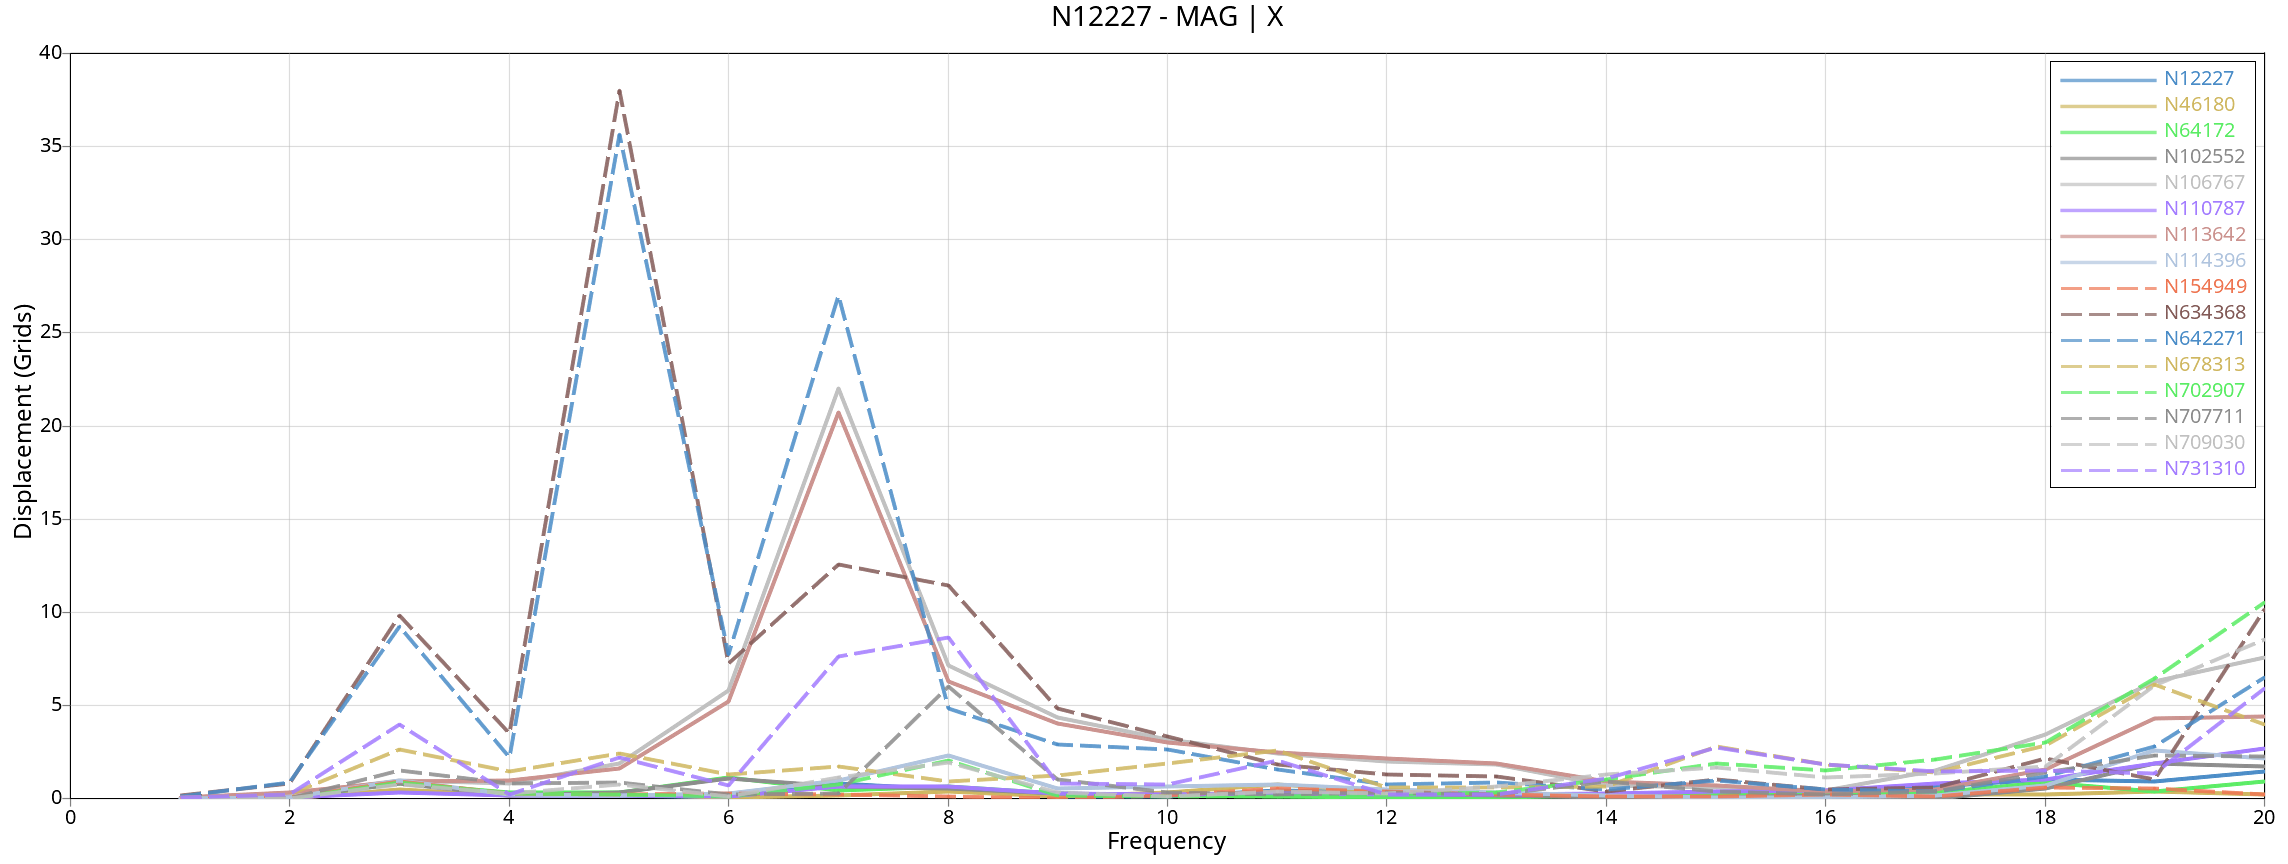
\includegraphics[width=0.7\linewidth]{pics/C020304_ax.png}
    \\
    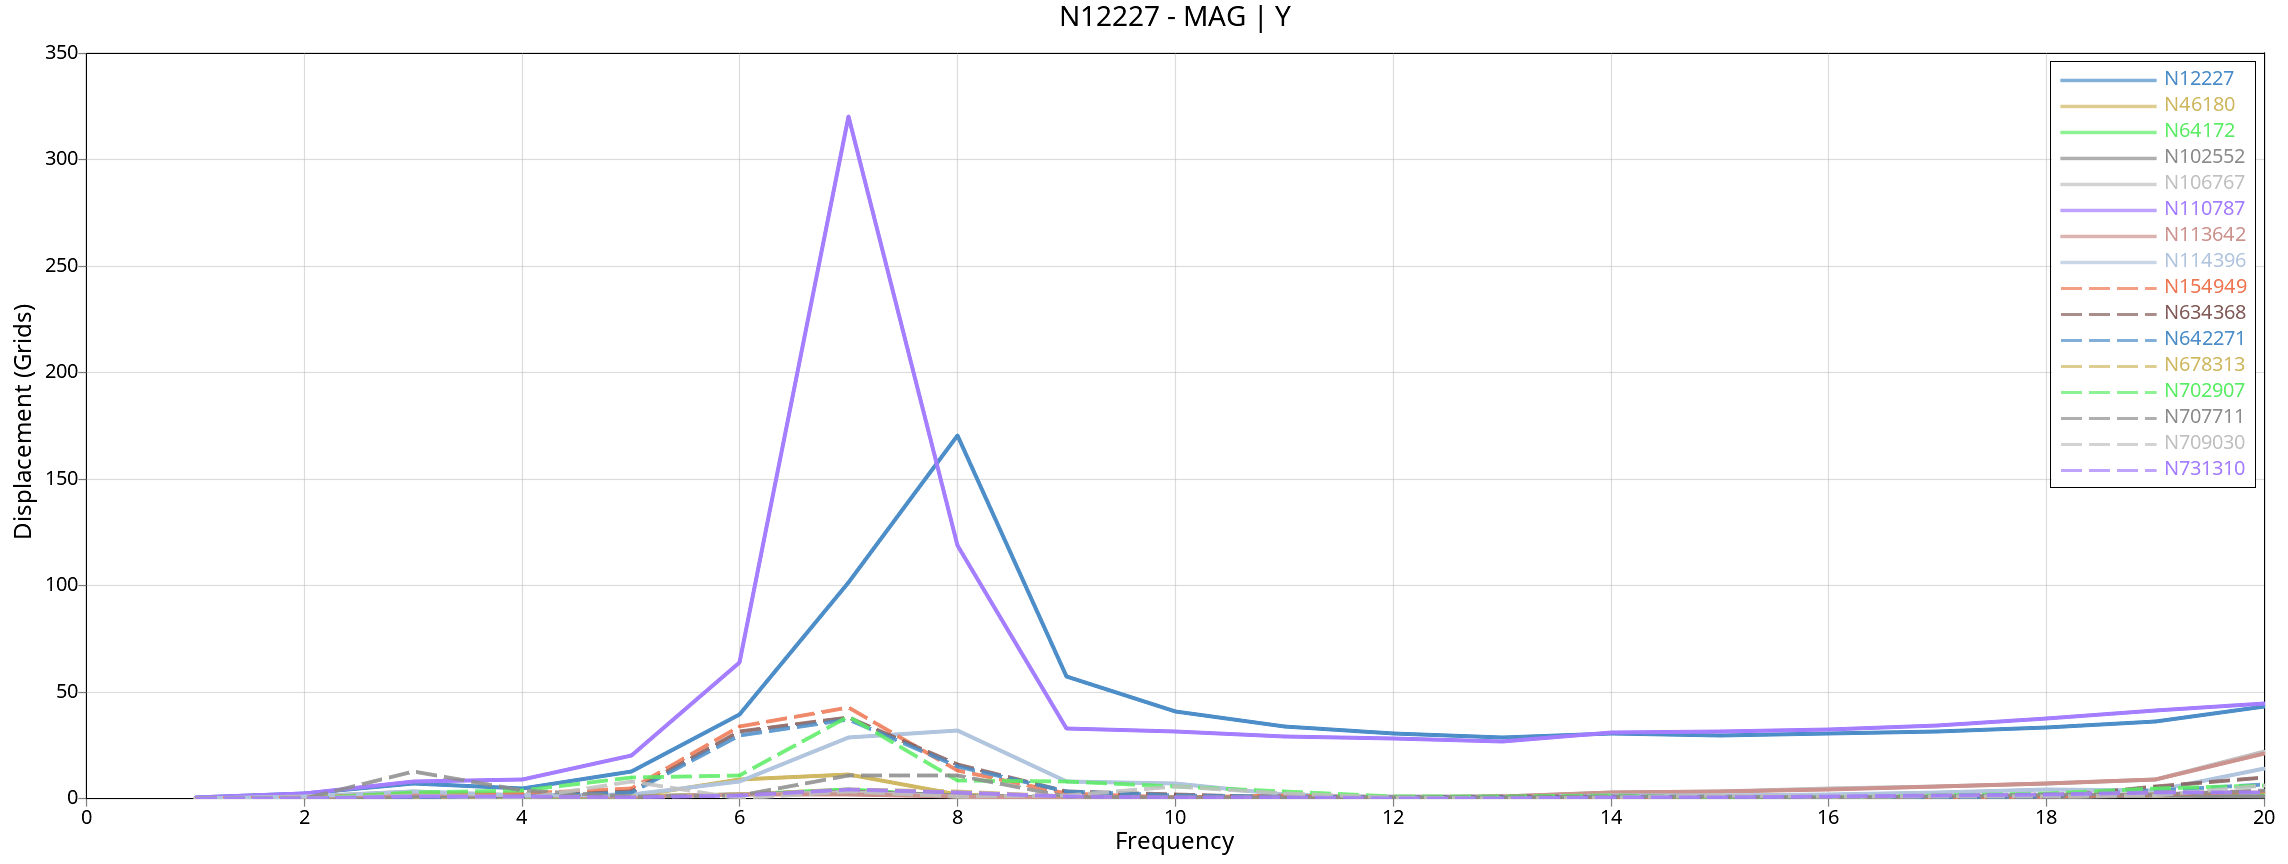
\includegraphics[width=0.7\linewidth]{pics/C020305_ay.png}
    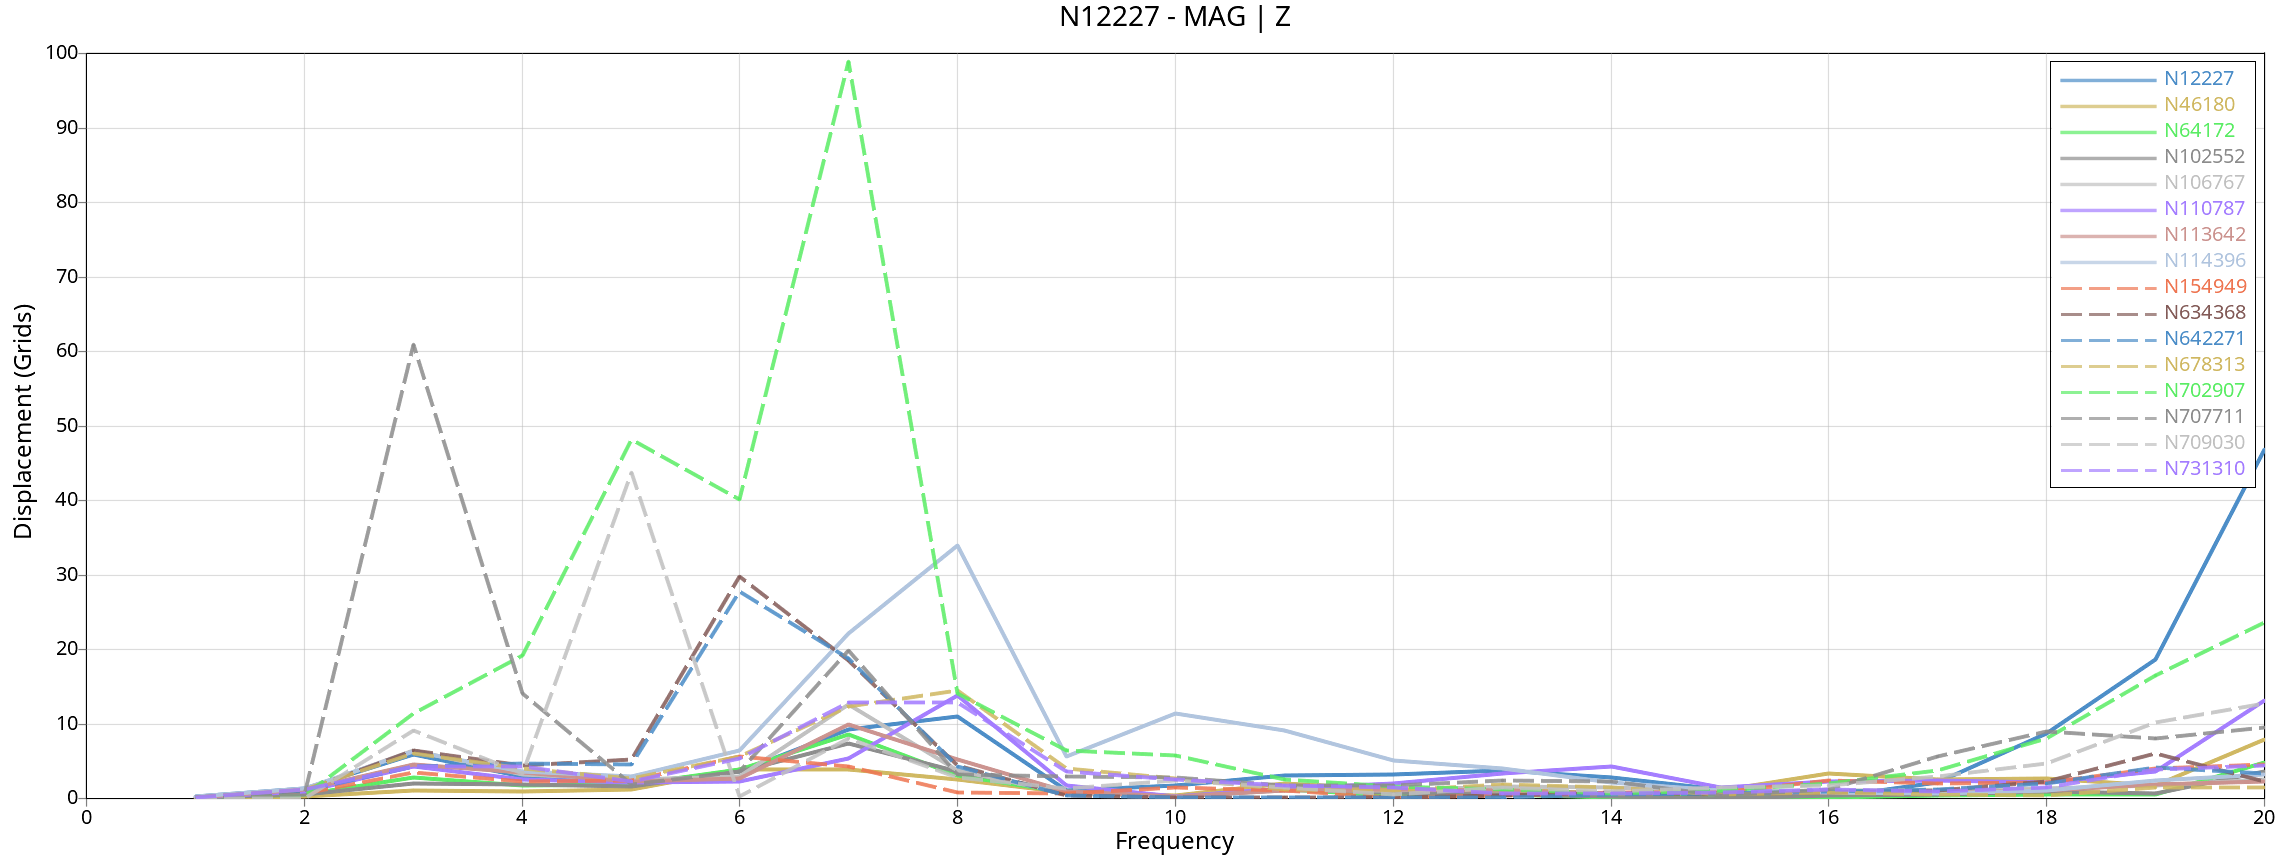
\includegraphics[width=0.7\linewidth]{pics/C020306_az.png}
    \captionsetup{labelformat=empty}
    \caption{\small{附图2.3: 动态特性分析 - 频率响应分析关键点结果输出}}
    \vspace{-0.4cm}
\end{figure}
\newpage{}
\par{}
\begin{figure}[h]
    \centering
    \vspace{-0.1cm}
    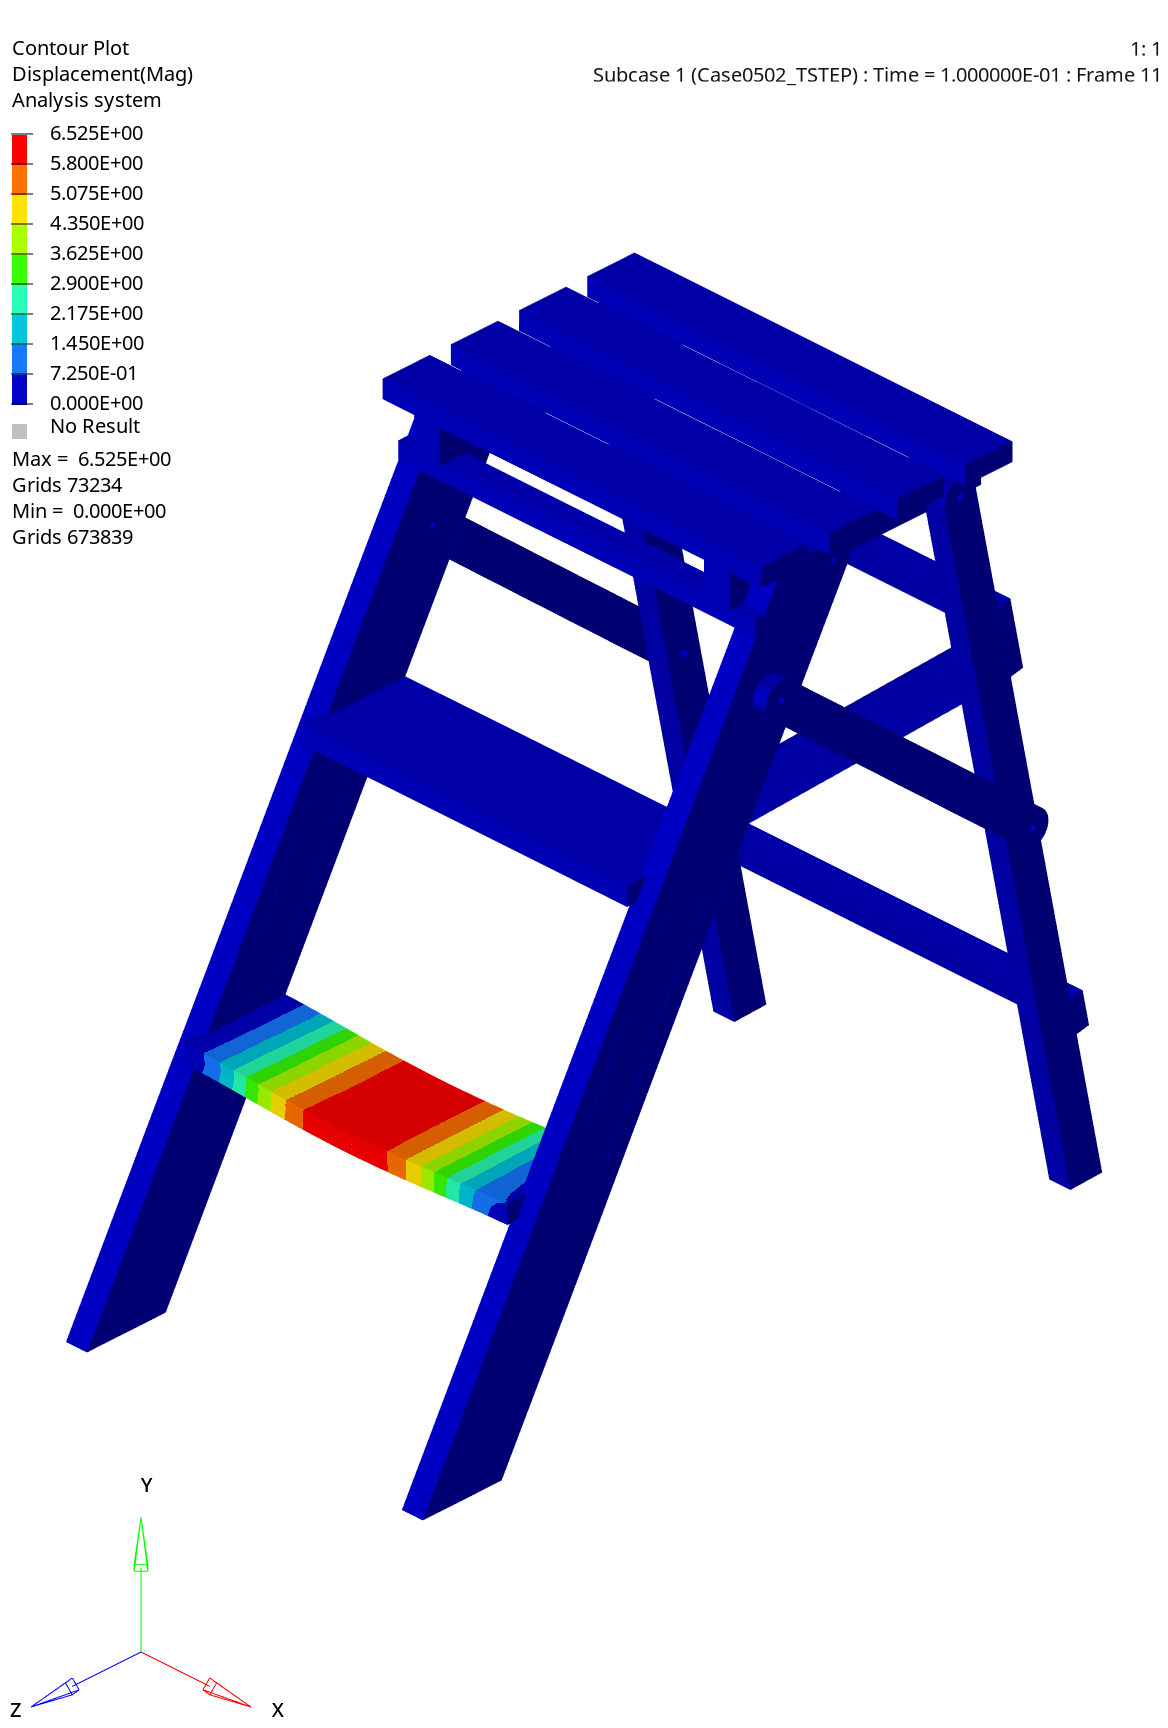
\includegraphics[width=0.32\linewidth]{pics/C020401.png}
    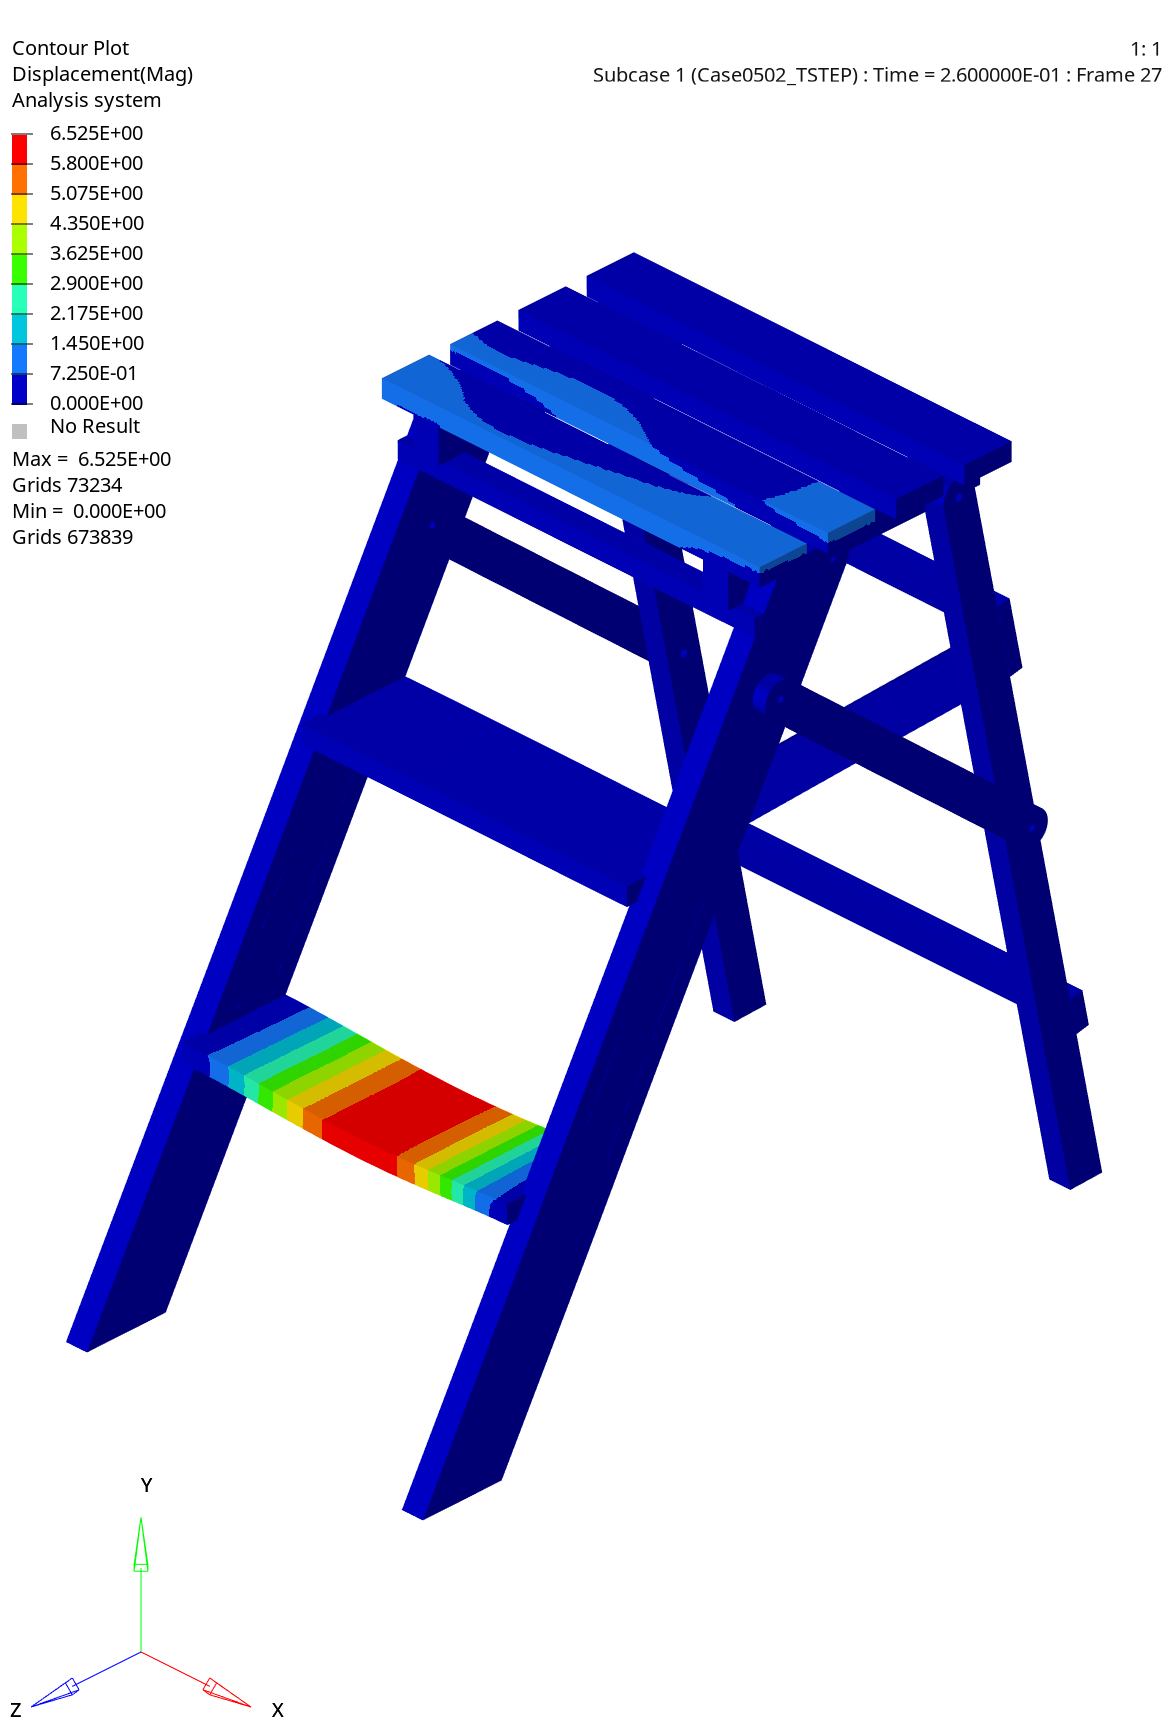
\includegraphics[width=0.32\linewidth]{pics/C020402.png}
    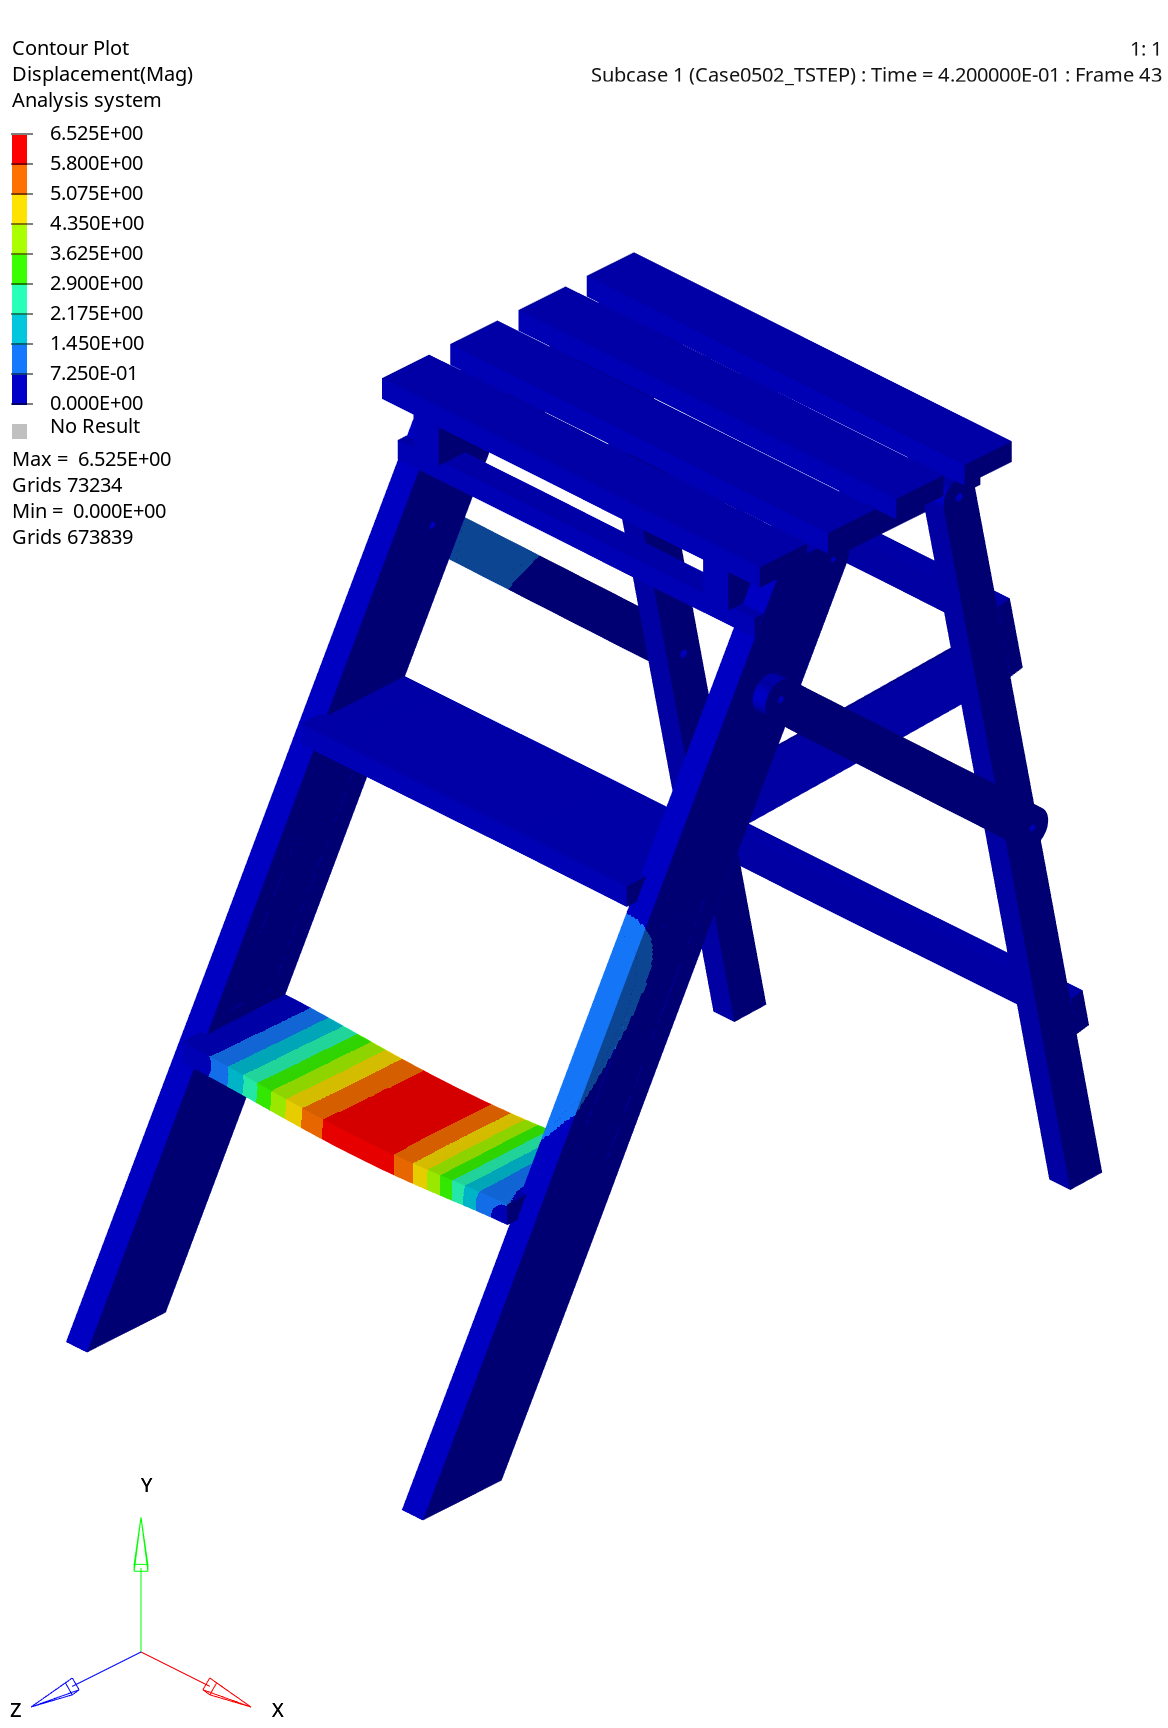
\includegraphics[width=0.32\linewidth]{pics/C020403.png}
    \\
    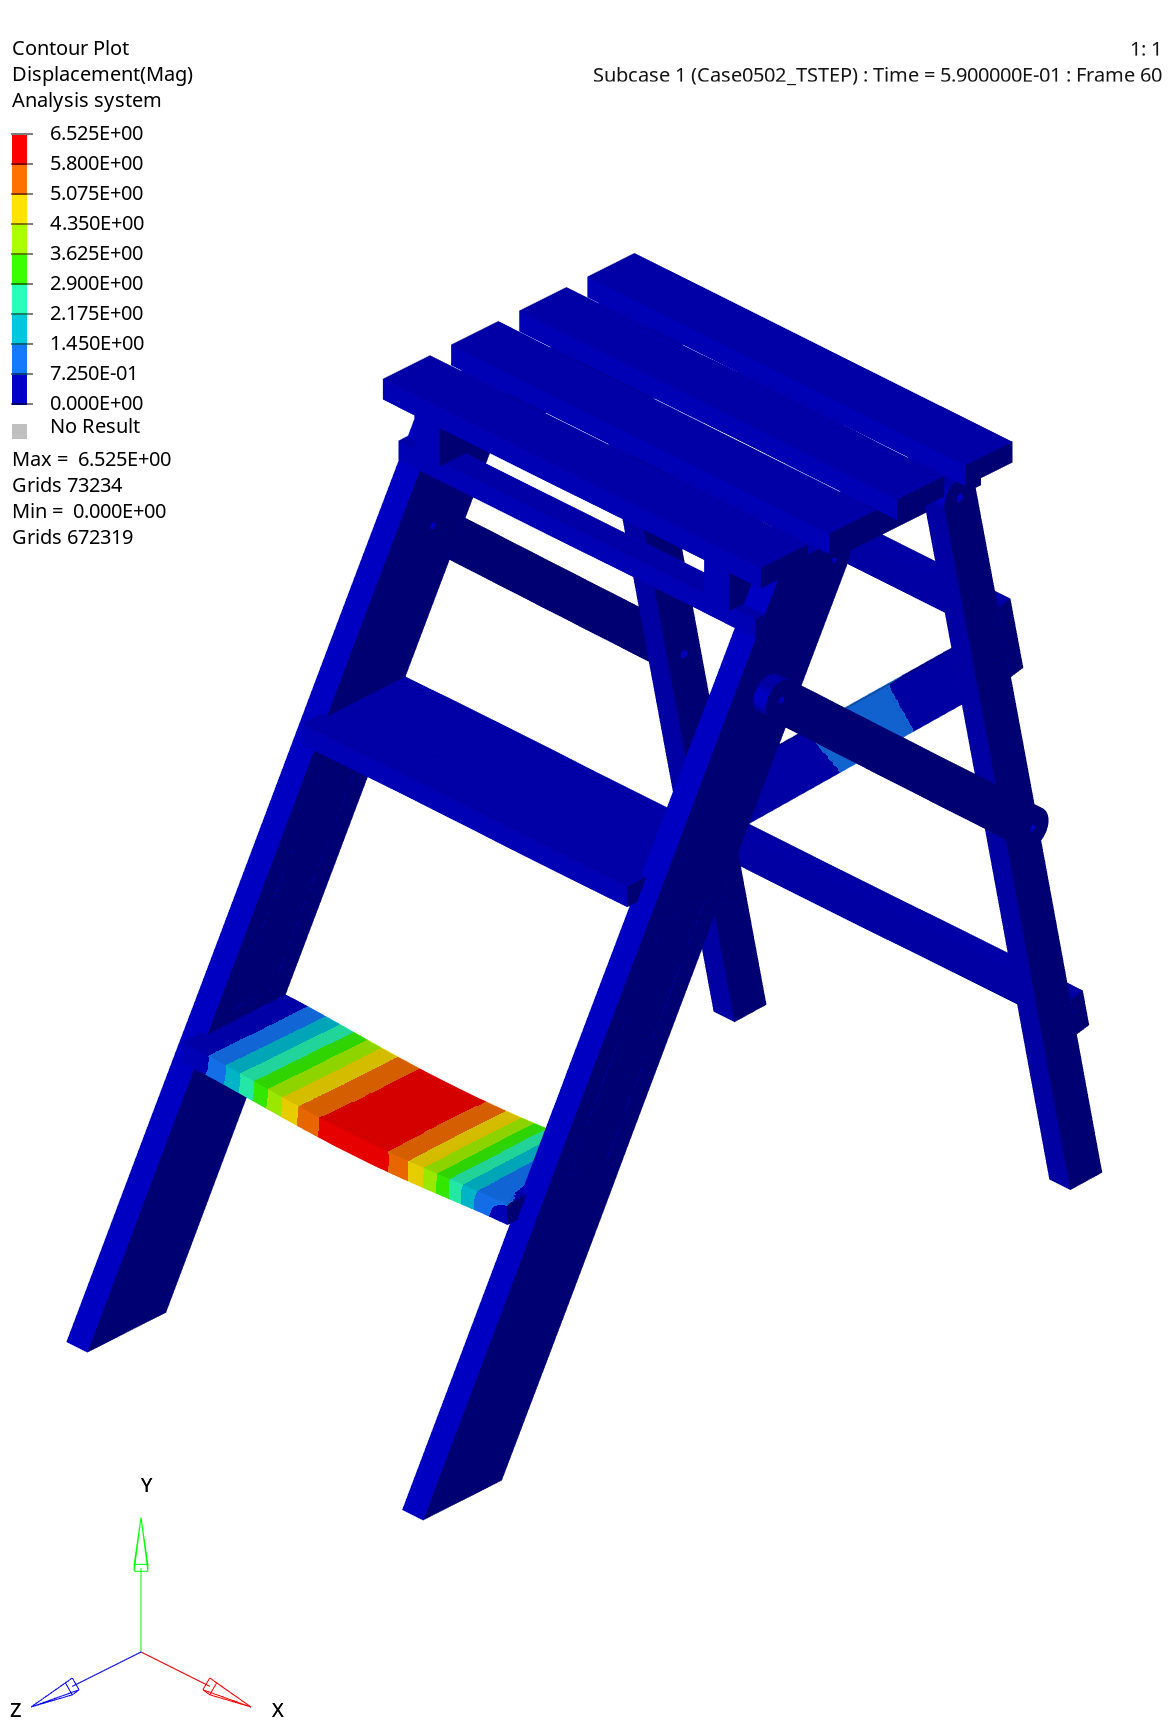
\includegraphics[width=0.32\linewidth]{pics/C020404.png}
    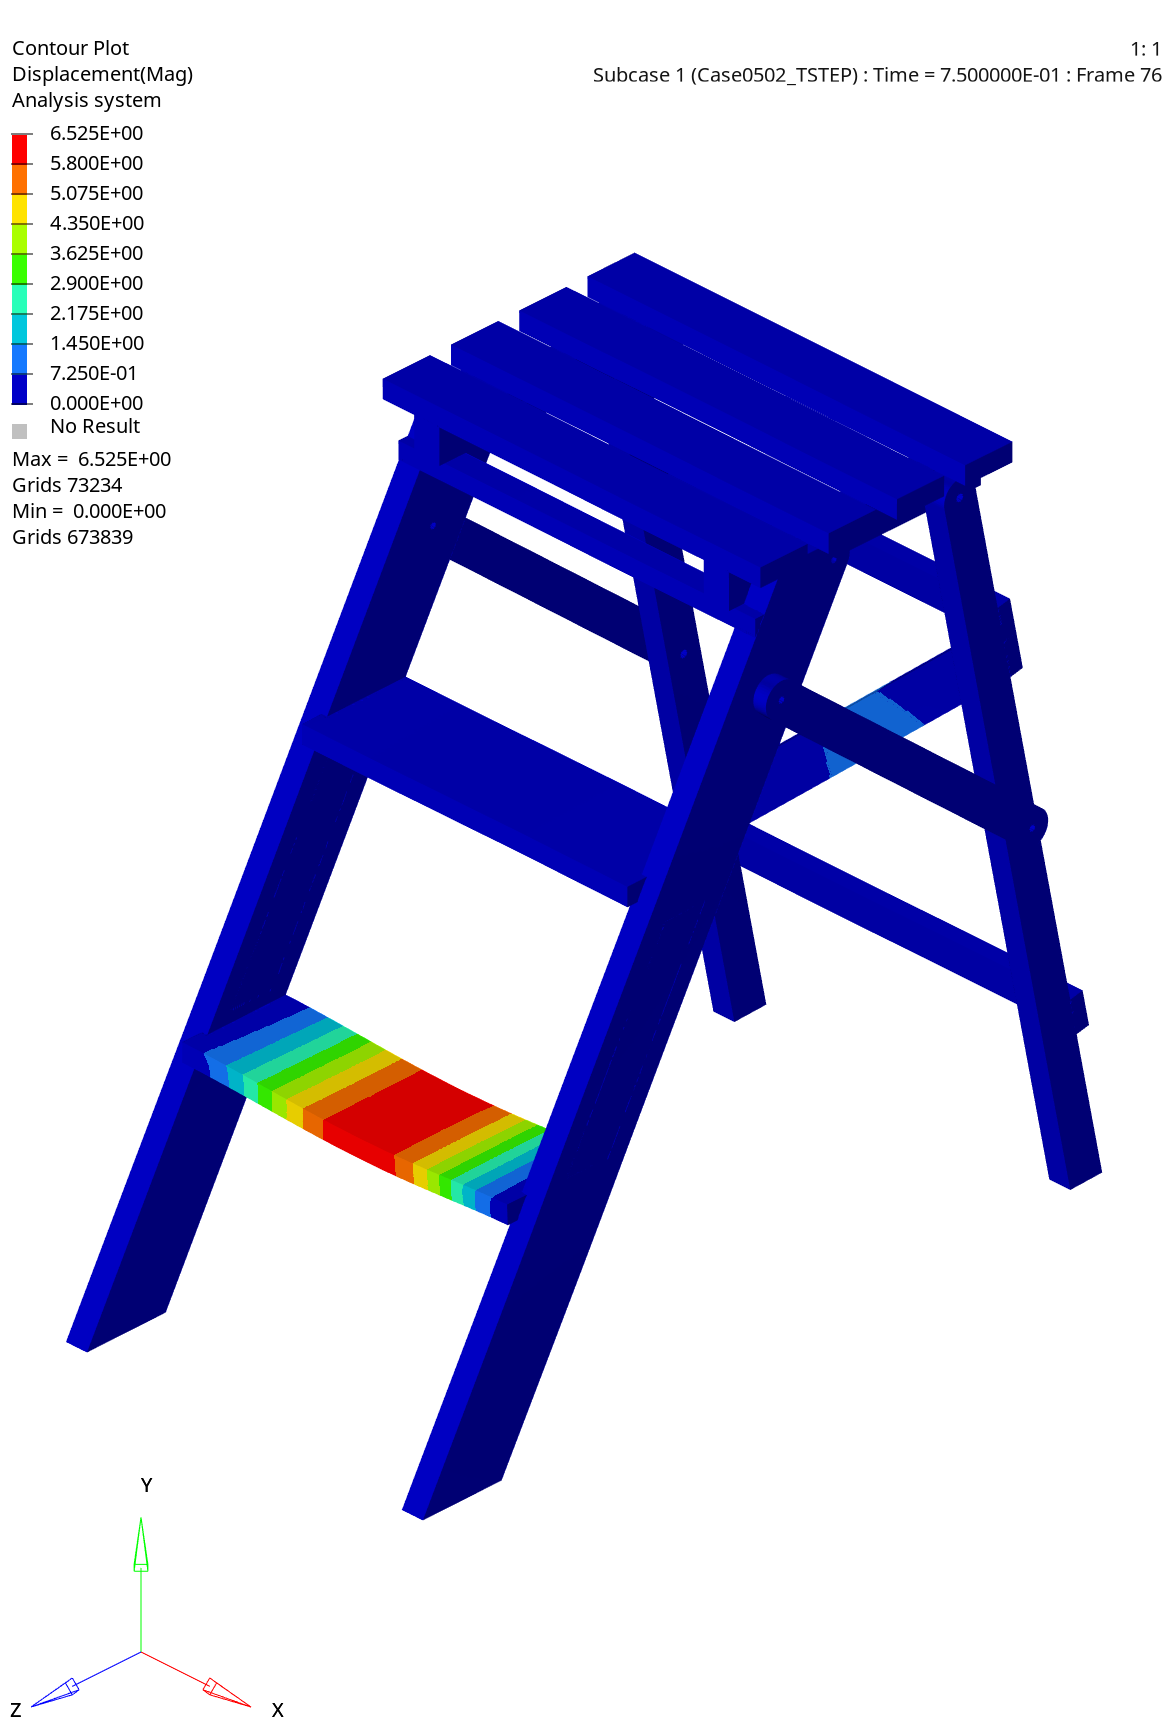
\includegraphics[width=0.32\linewidth]{pics/C020405.png}
    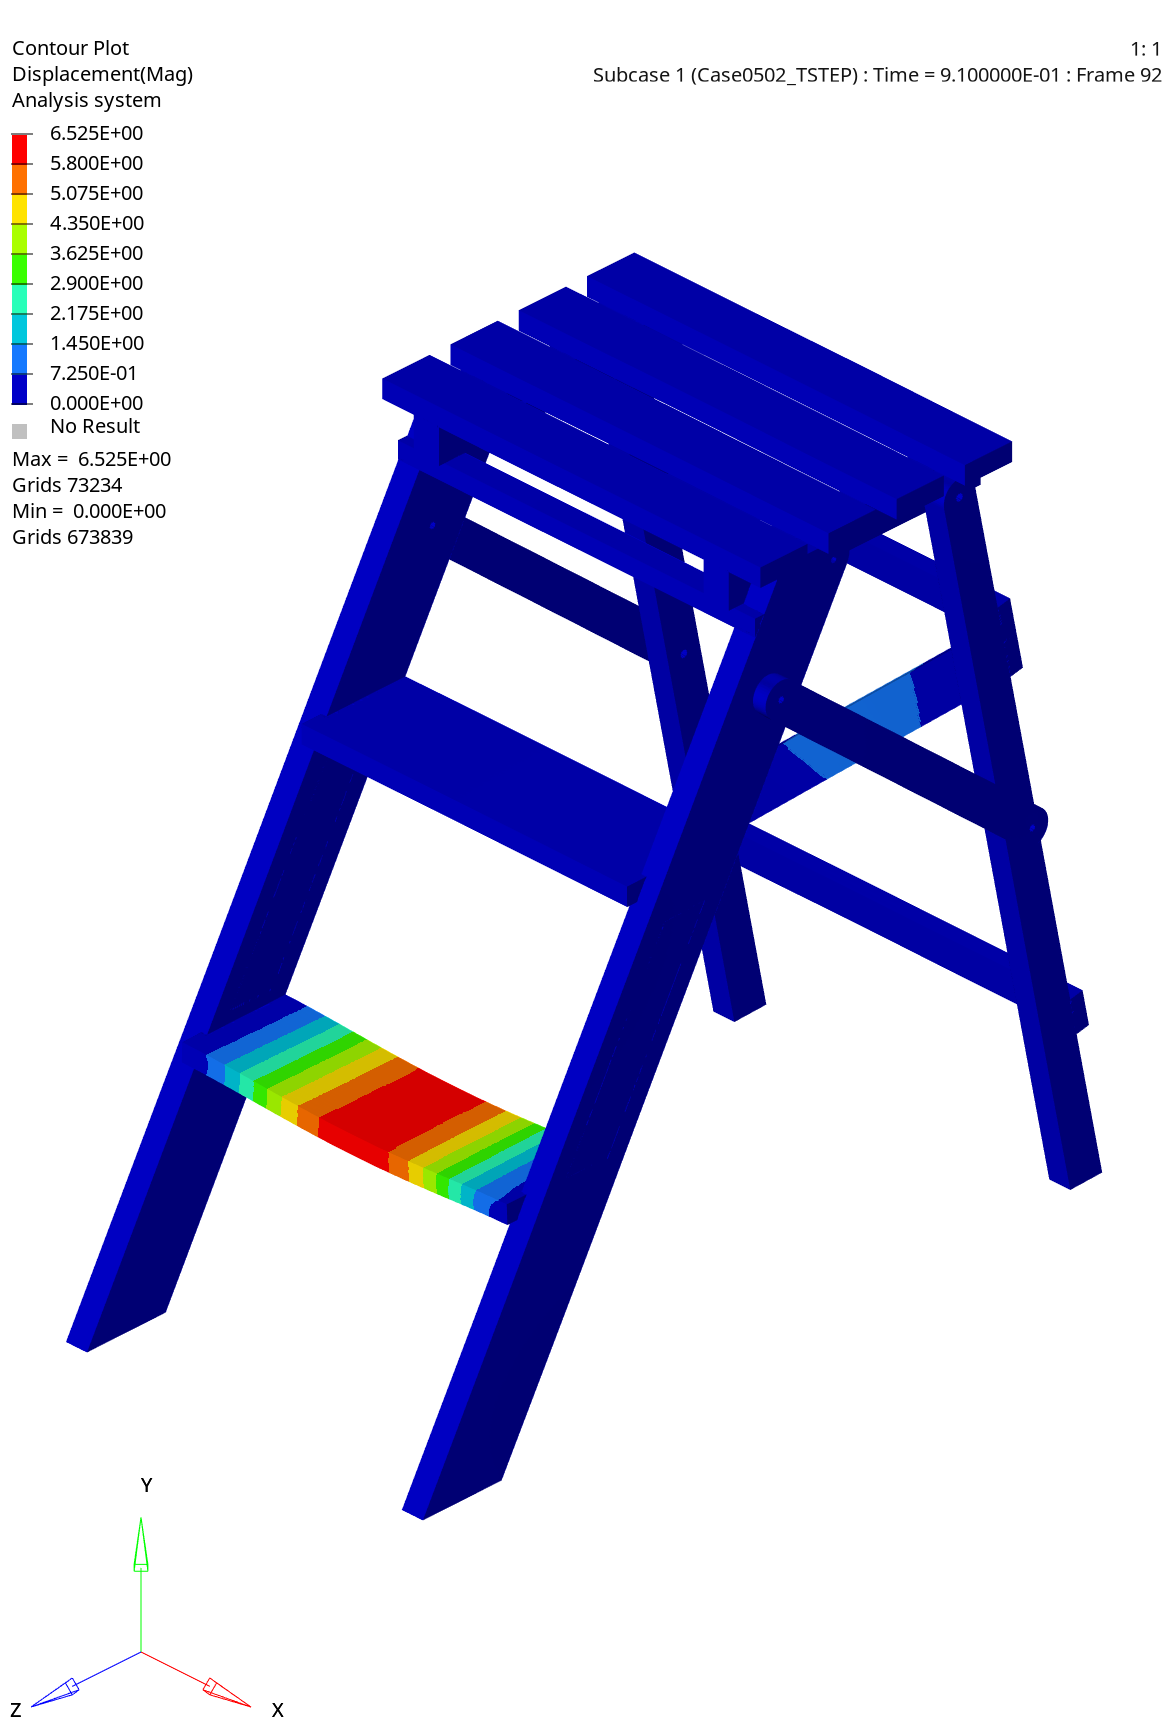
\includegraphics[width=0.32\linewidth]{pics/C020406.png}
    \\
    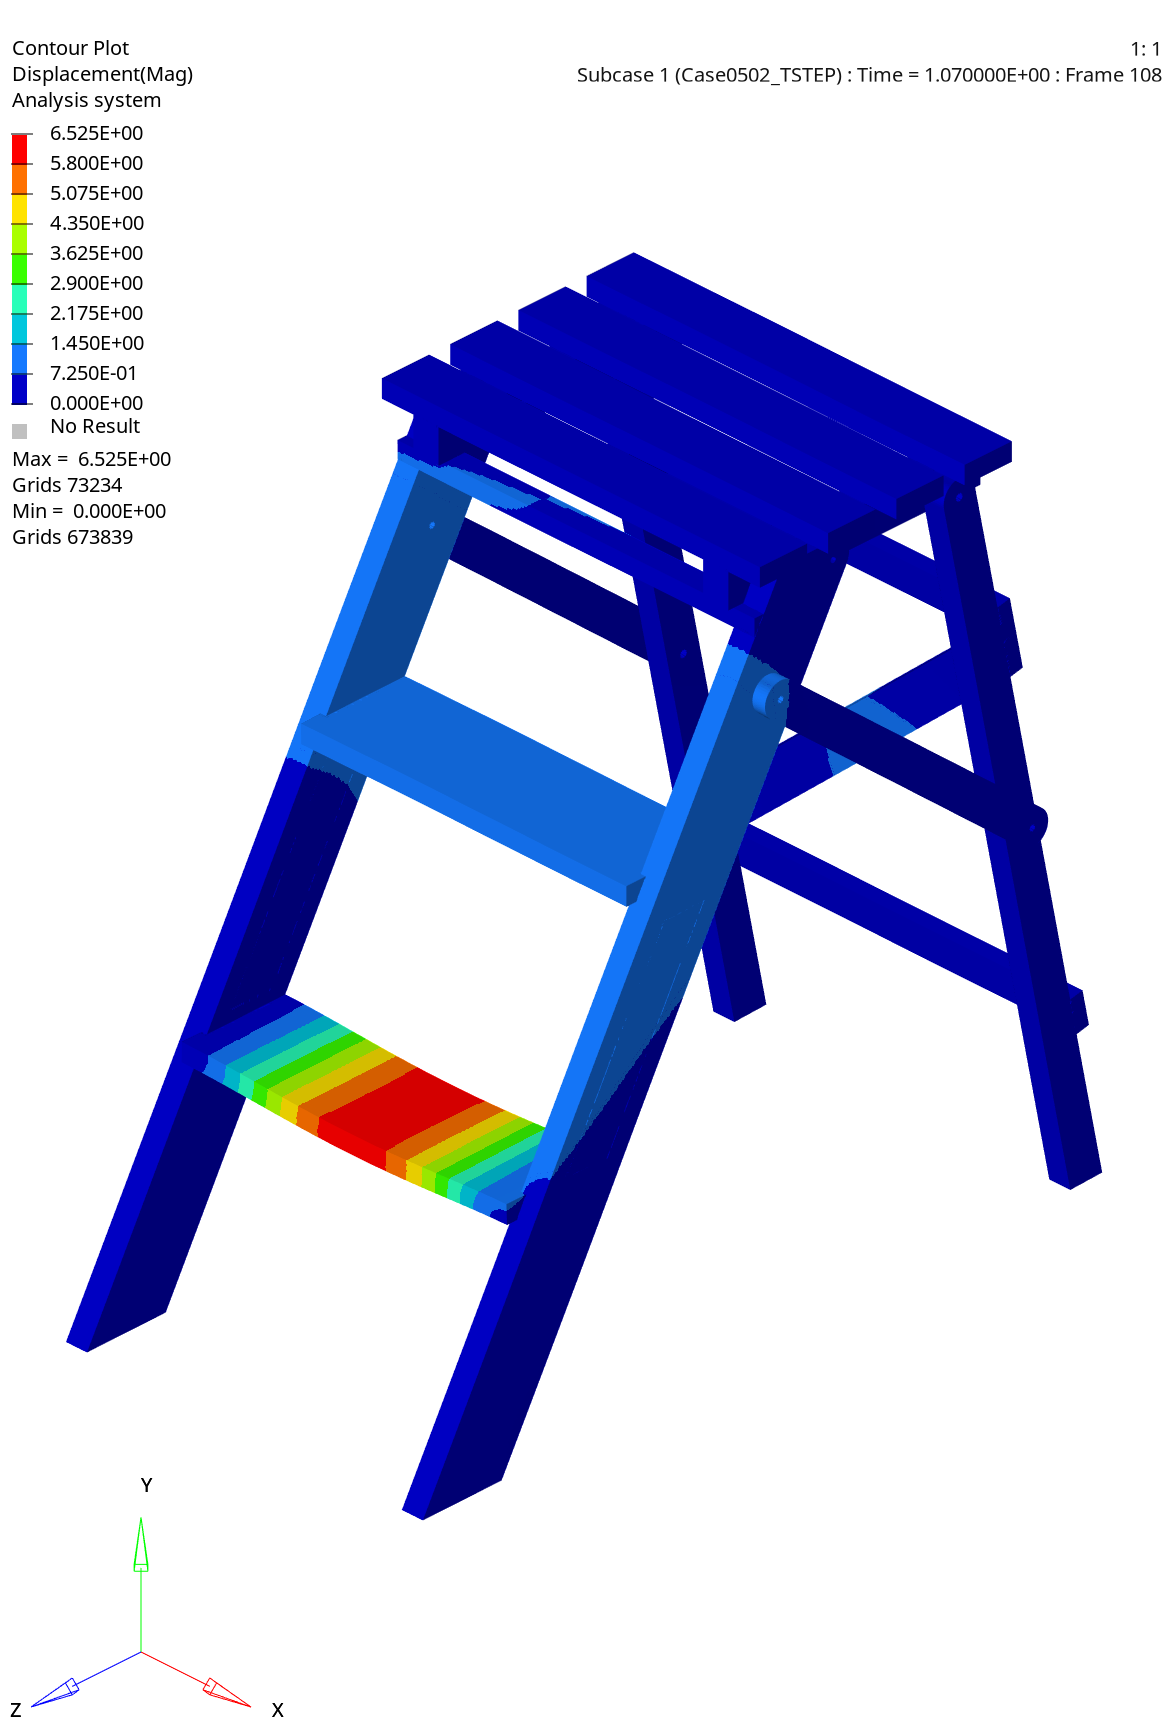
\includegraphics[width=0.32\linewidth]{pics/C020407.png}
    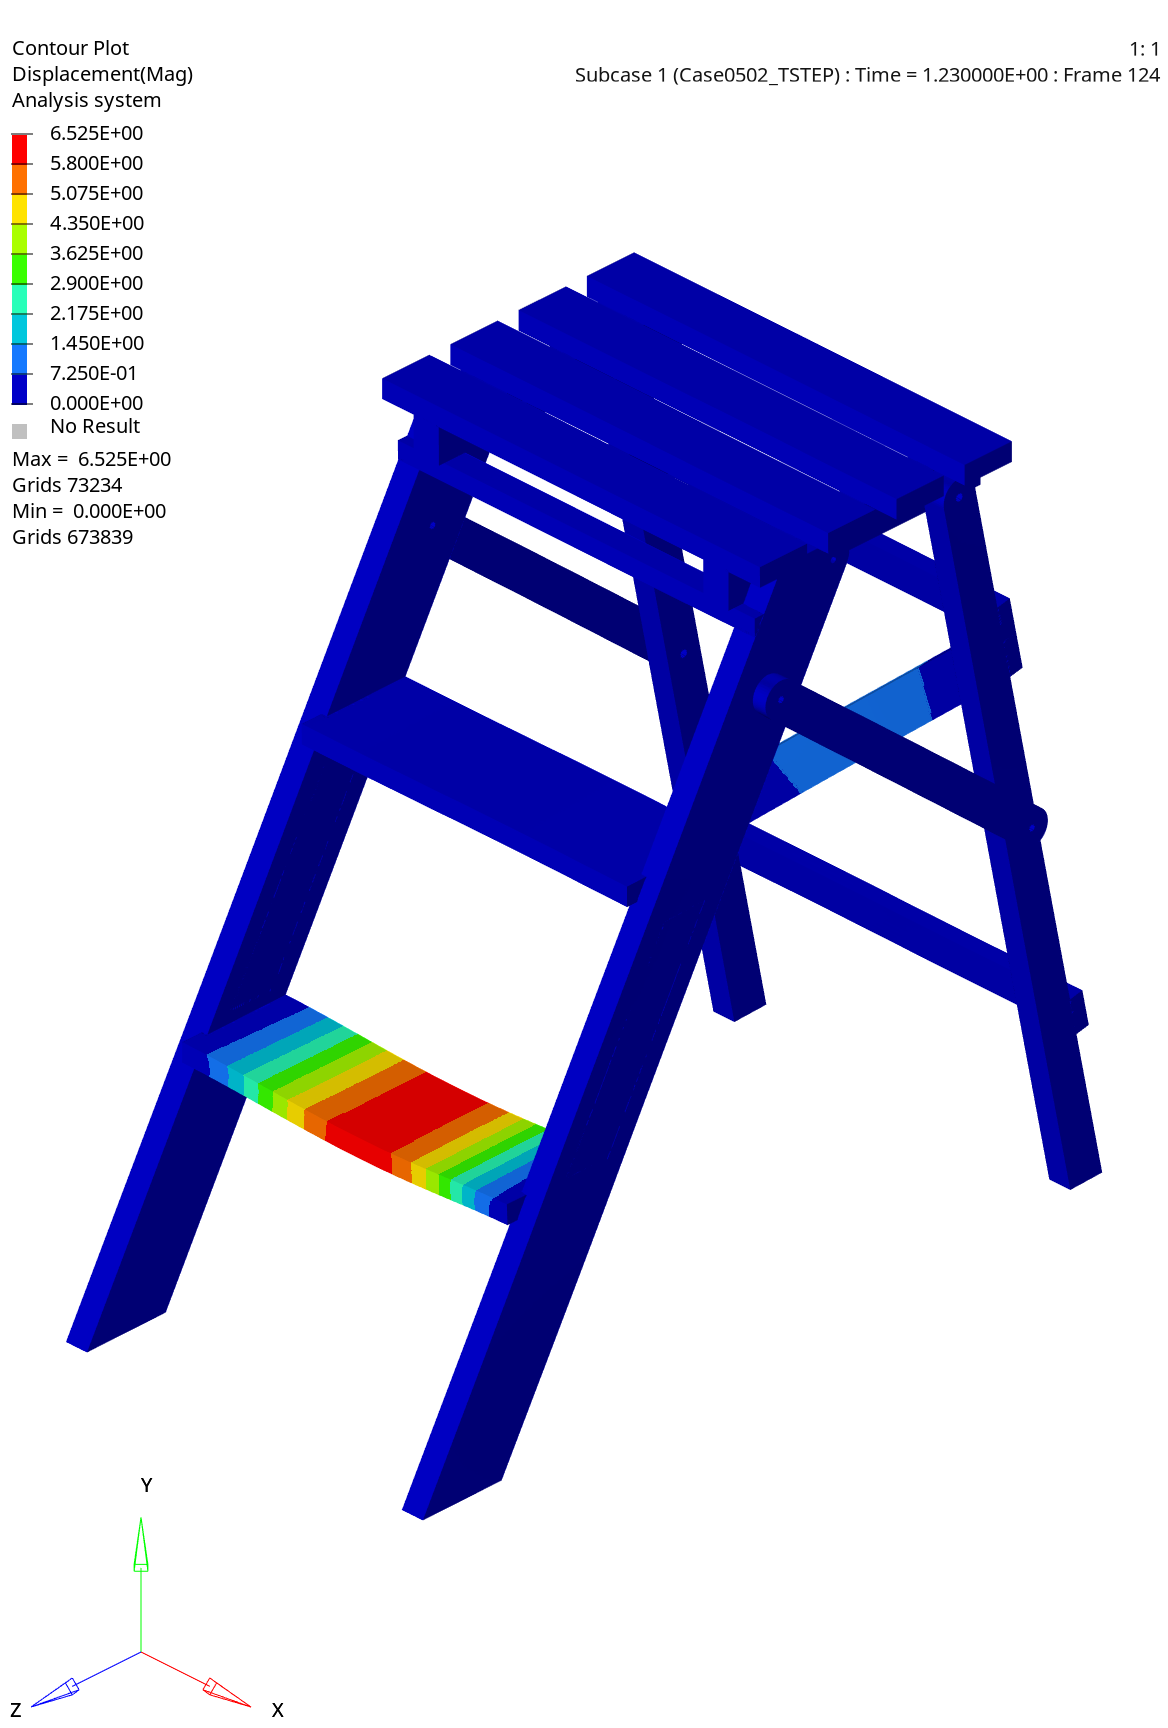
\includegraphics[width=0.32\linewidth]{pics/C020408.png}
    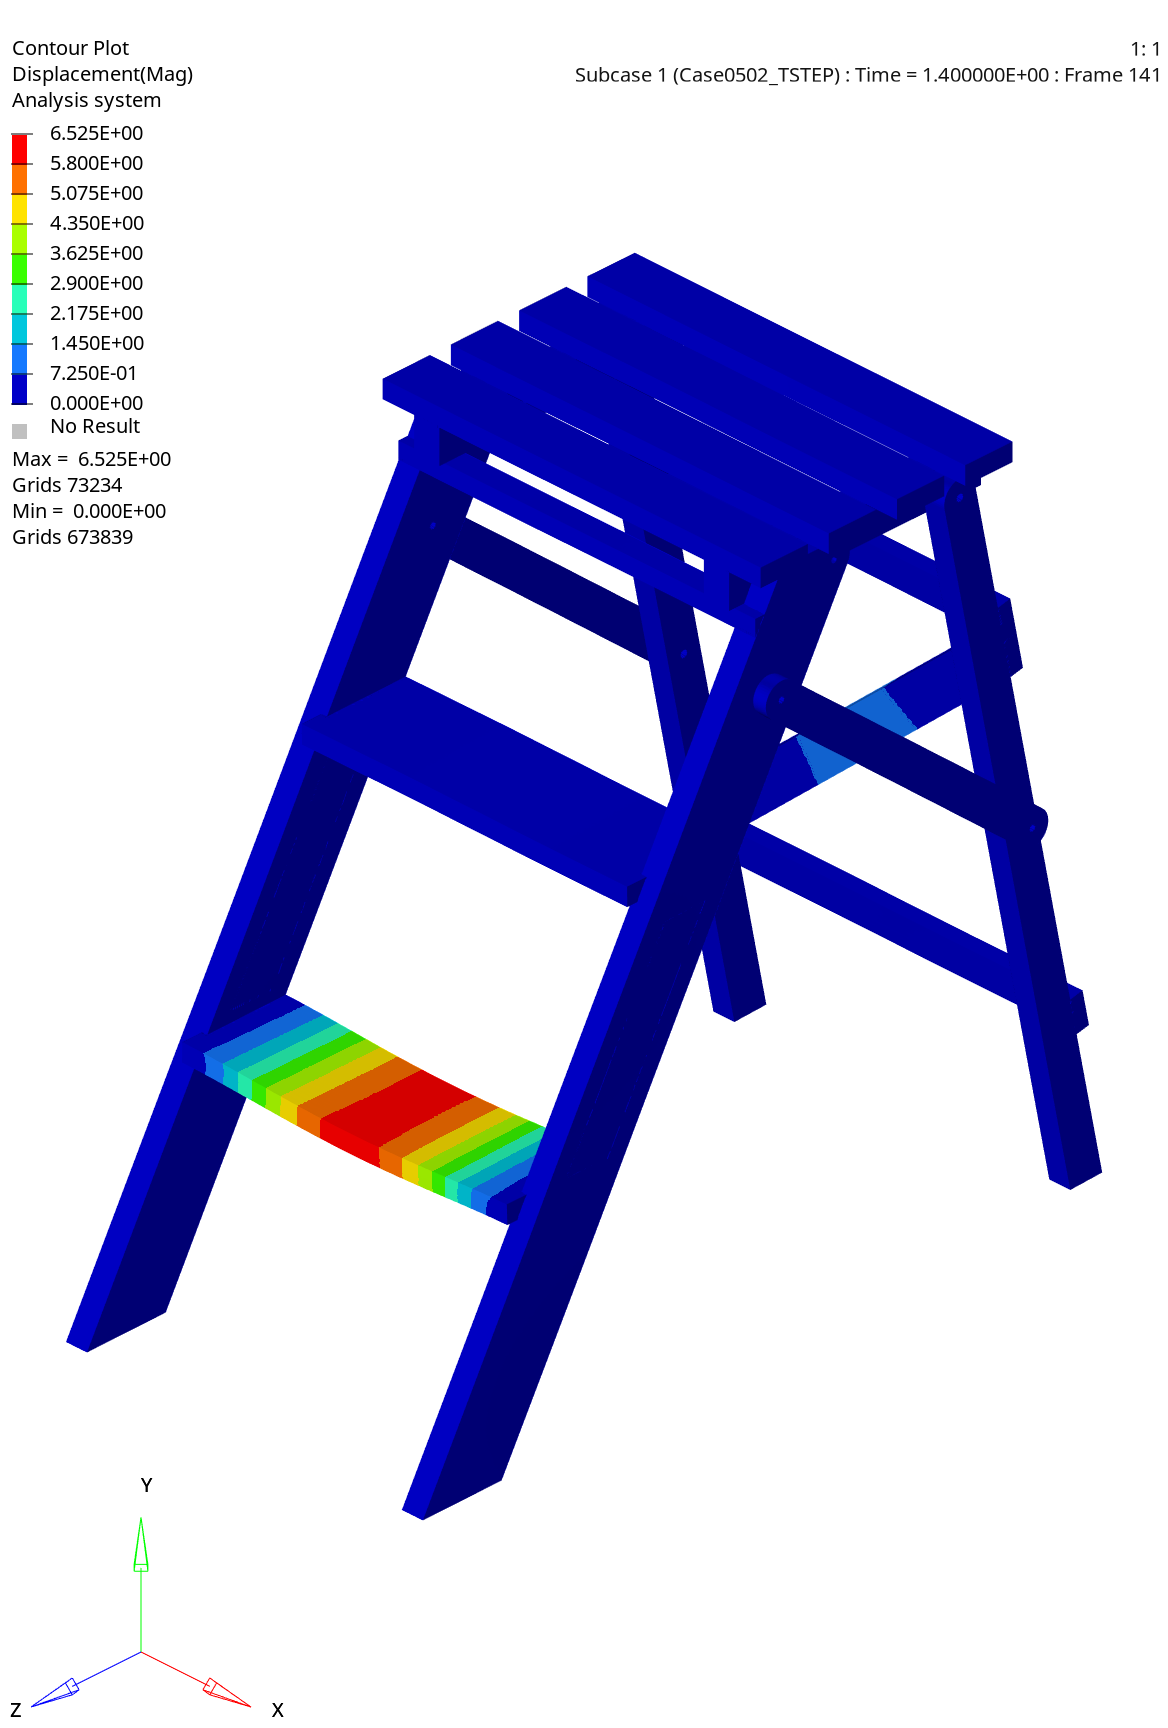
\includegraphics[width=0.32\linewidth]{pics/C020409.png}
    \captionsetup{labelformat=empty}
    \caption{\small{附图2.4.1: 动态特性分析 - 瞬态分析关键点结果输出 - 前9次}}
    \vspace{-0.4cm}
\end{figure}
\newpage{}
\par{}
\begin{figure}[h]
    \centering
    \vspace{-0.1cm}
    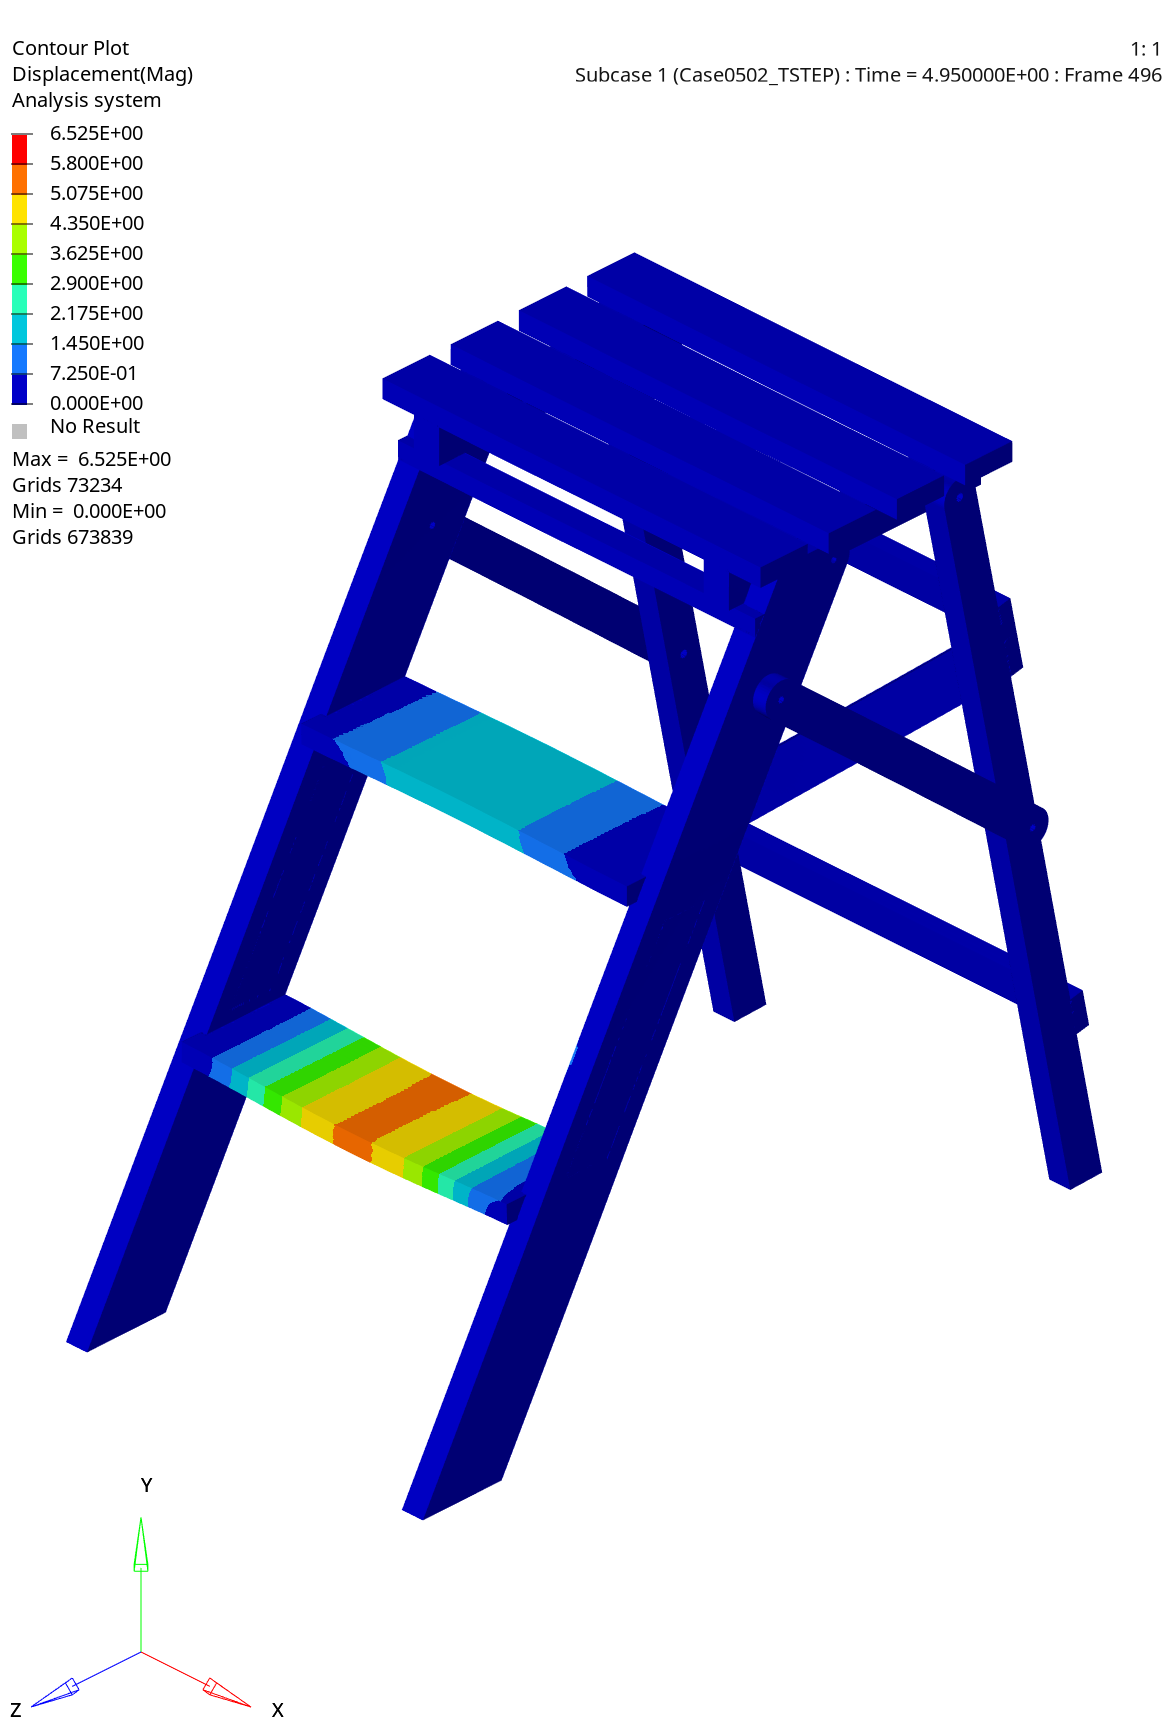
\includegraphics[width=0.32\linewidth]{pics/C020410.png}
    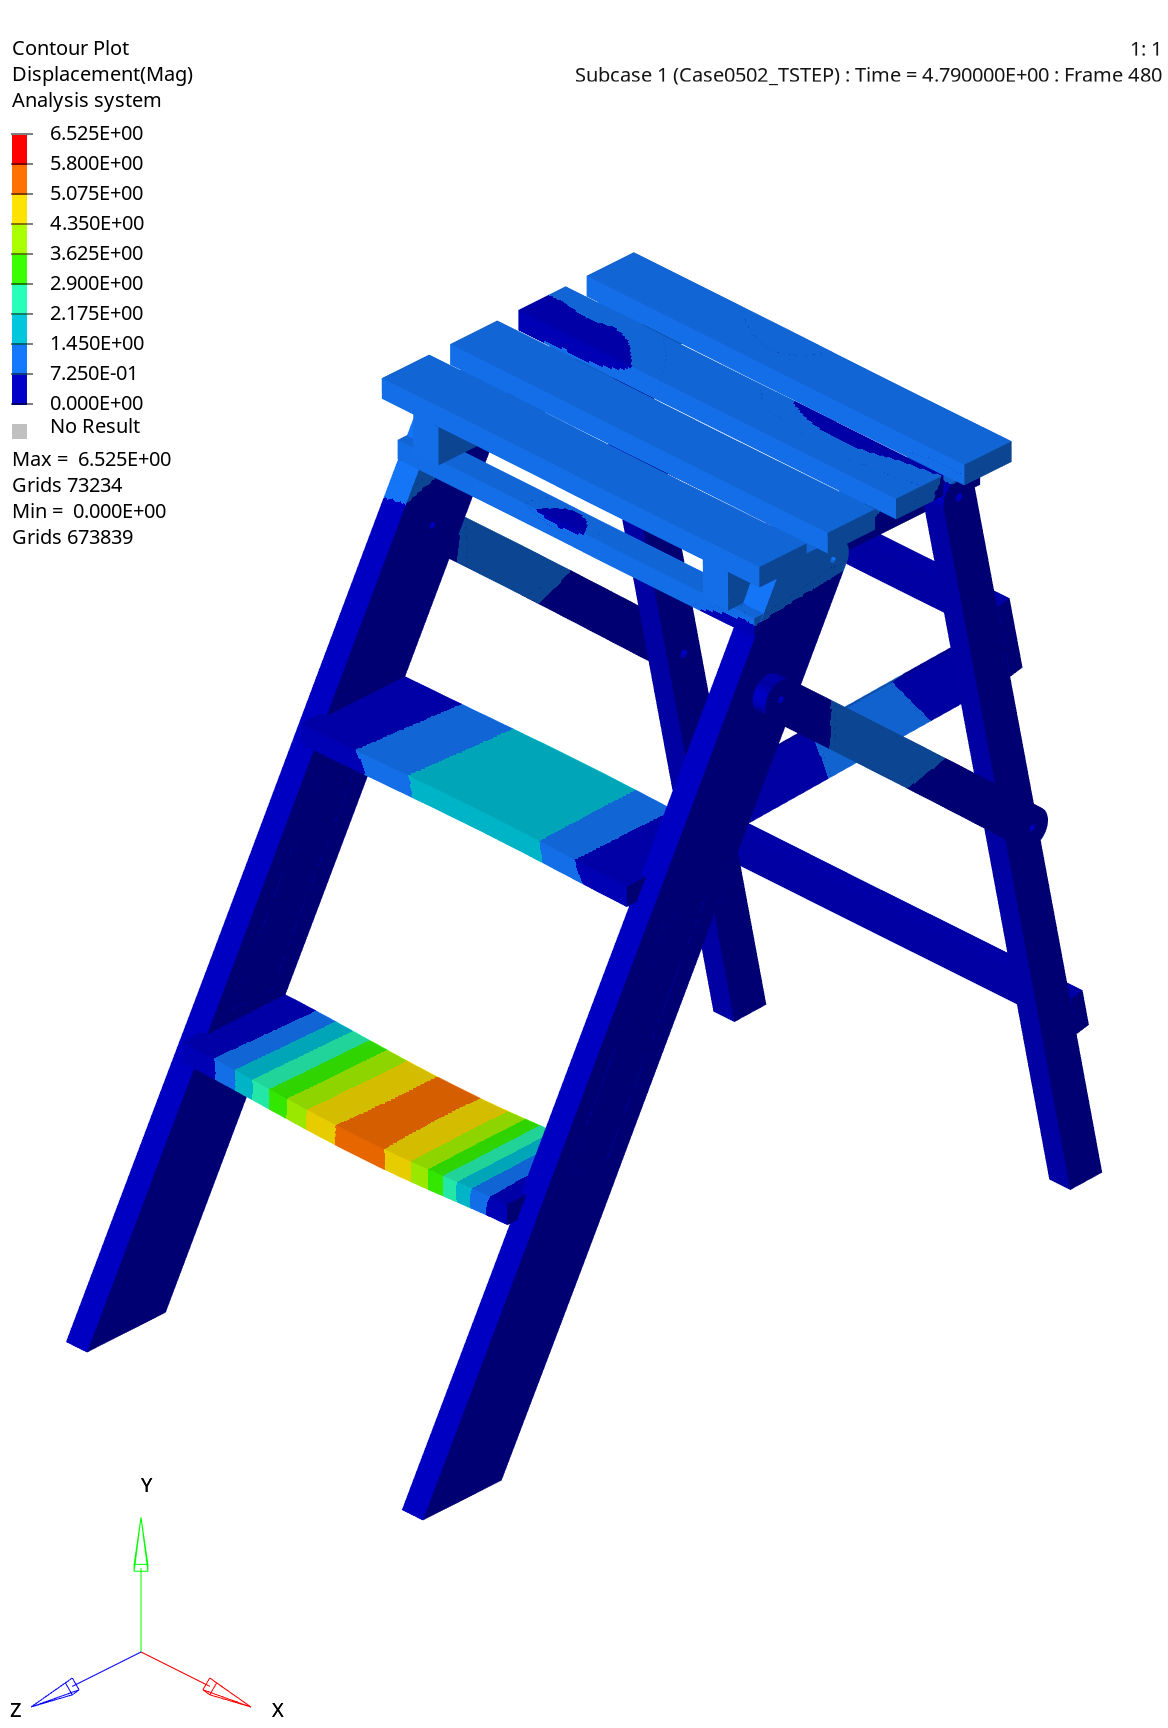
\includegraphics[width=0.32\linewidth]{pics/C020411.png}
    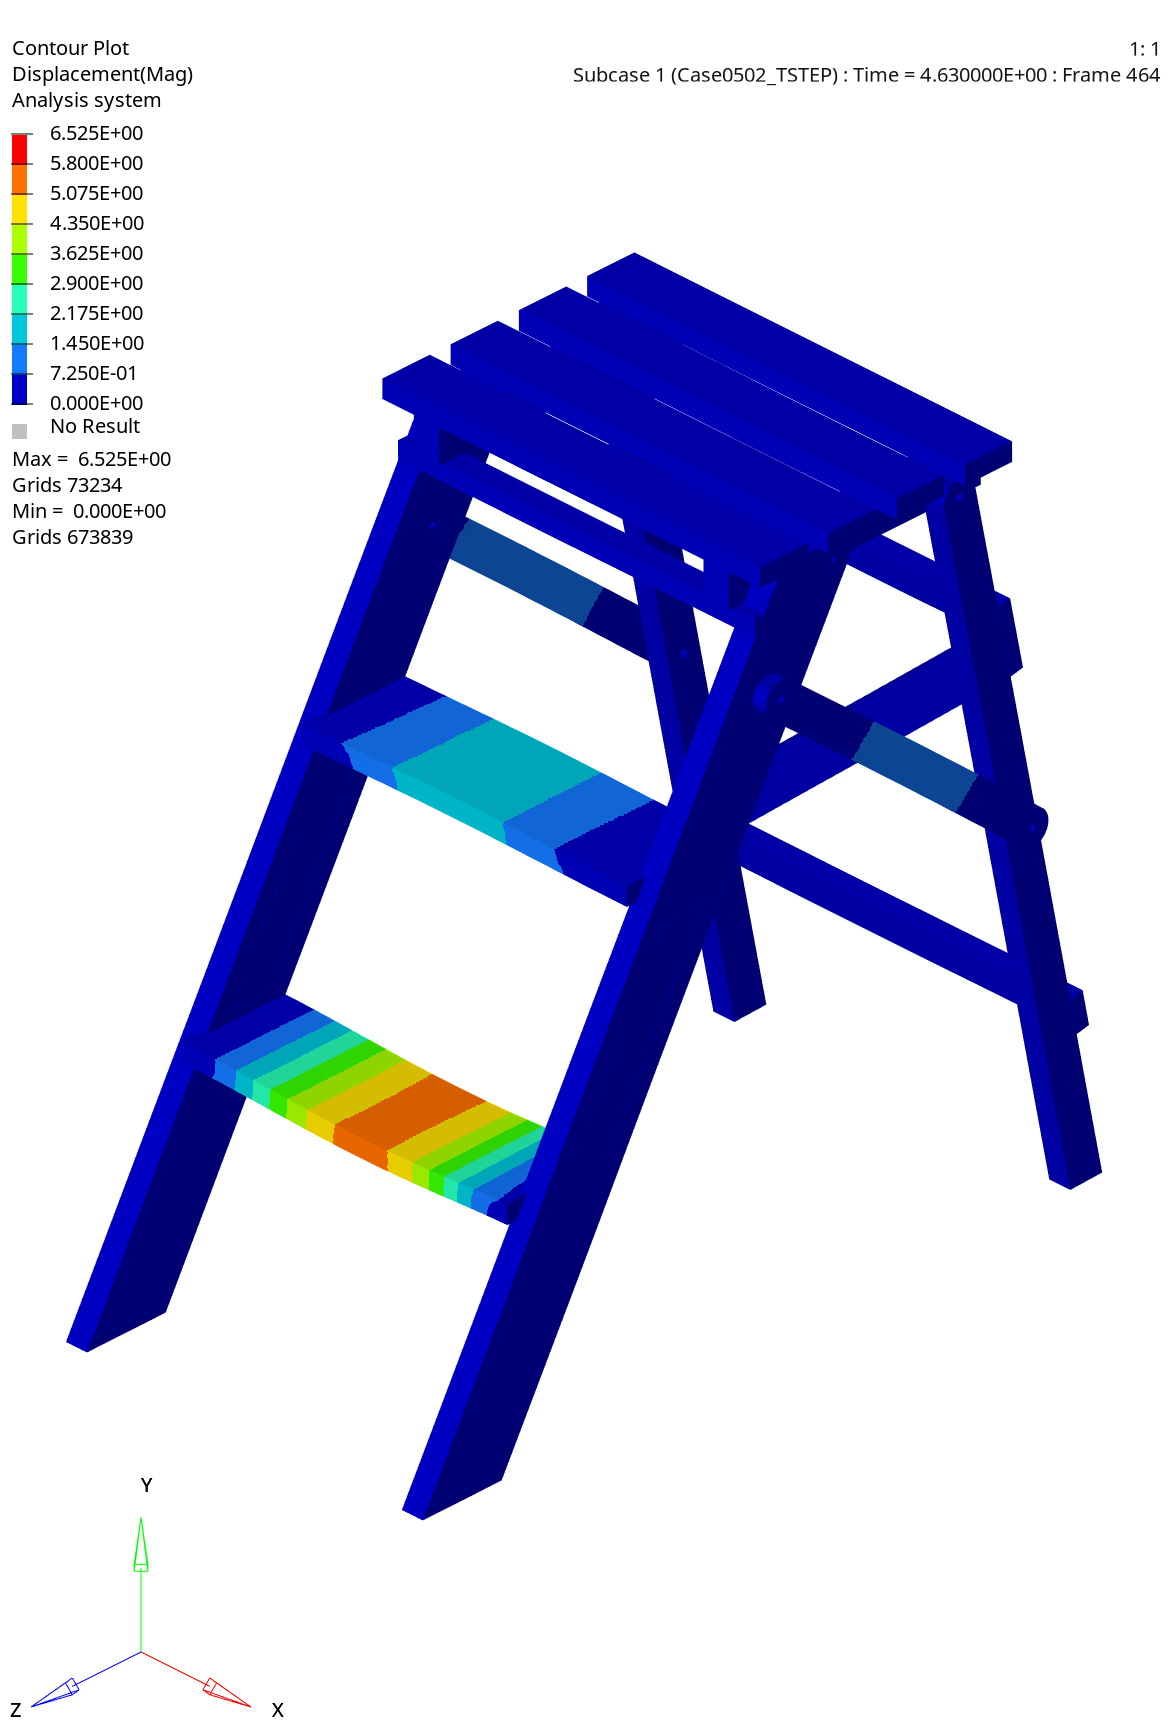
\includegraphics[width=0.32\linewidth]{pics/C020412.png}
    \\
    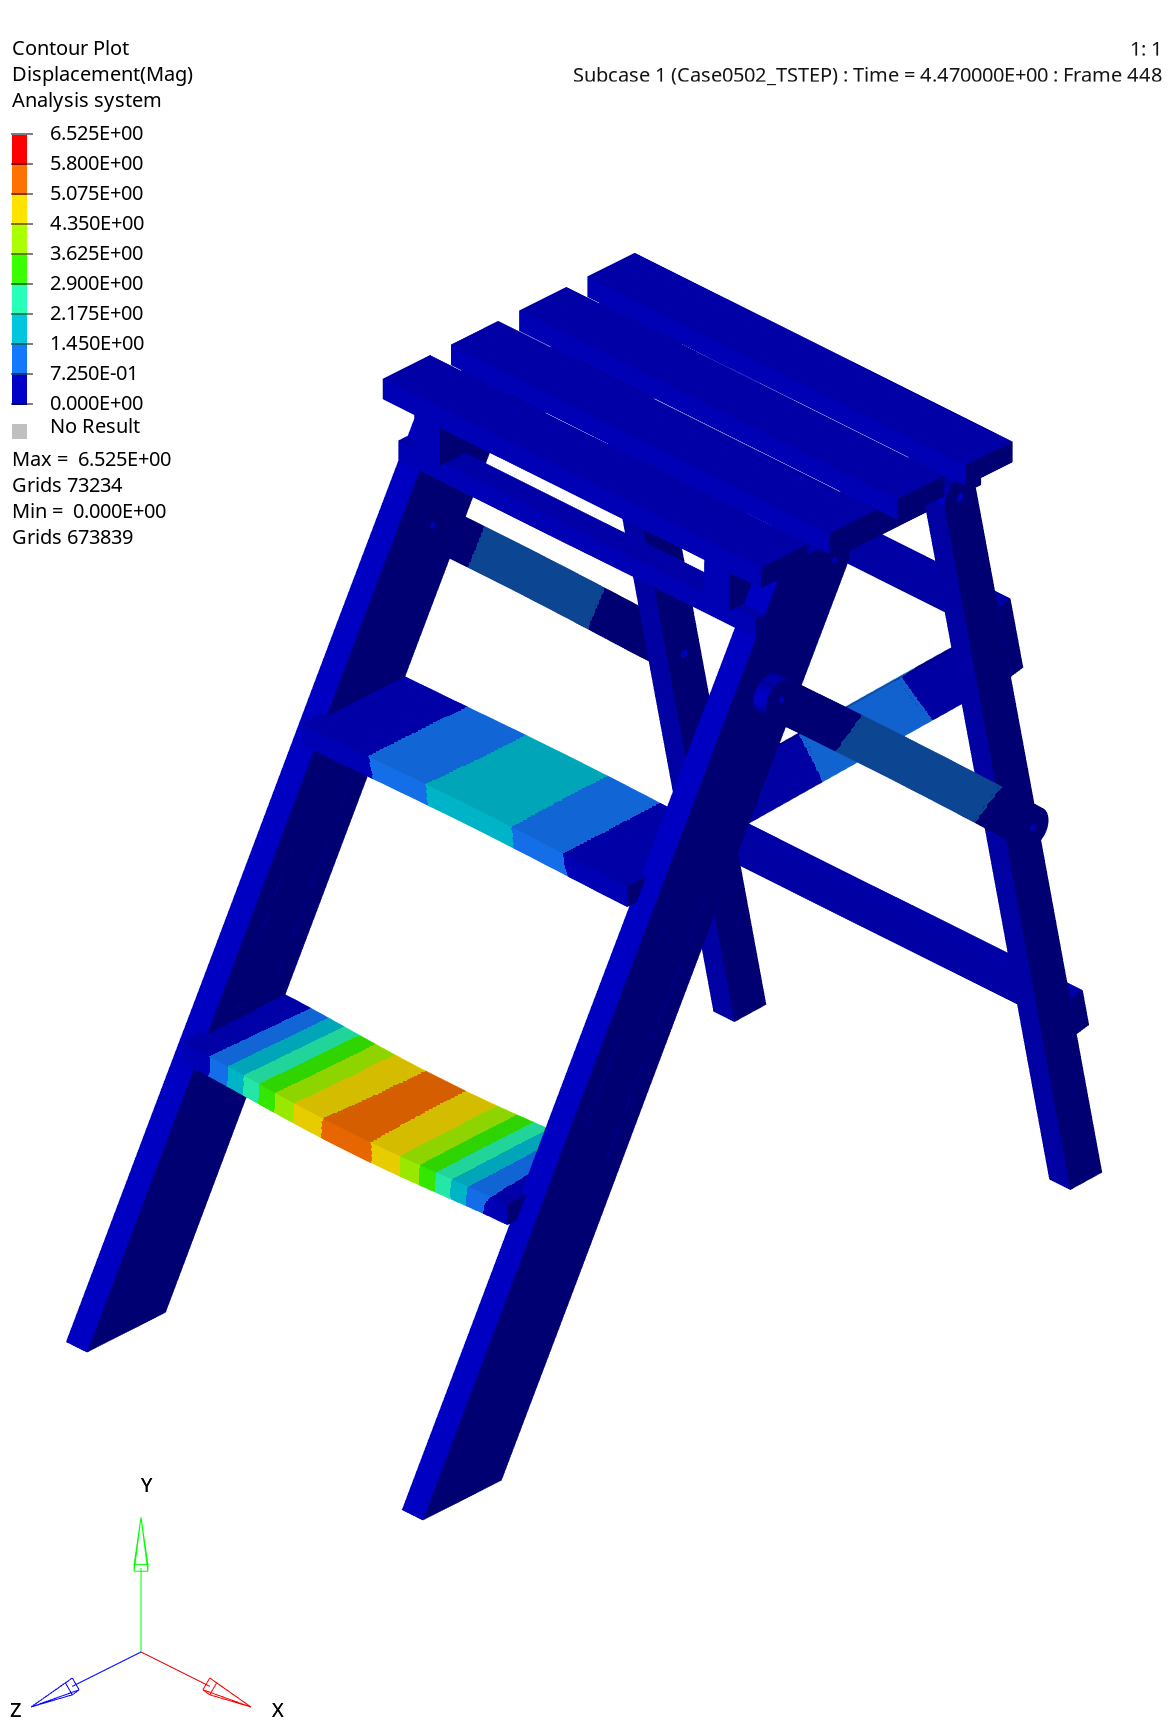
\includegraphics[width=0.32\linewidth]{pics/C020413.png}
    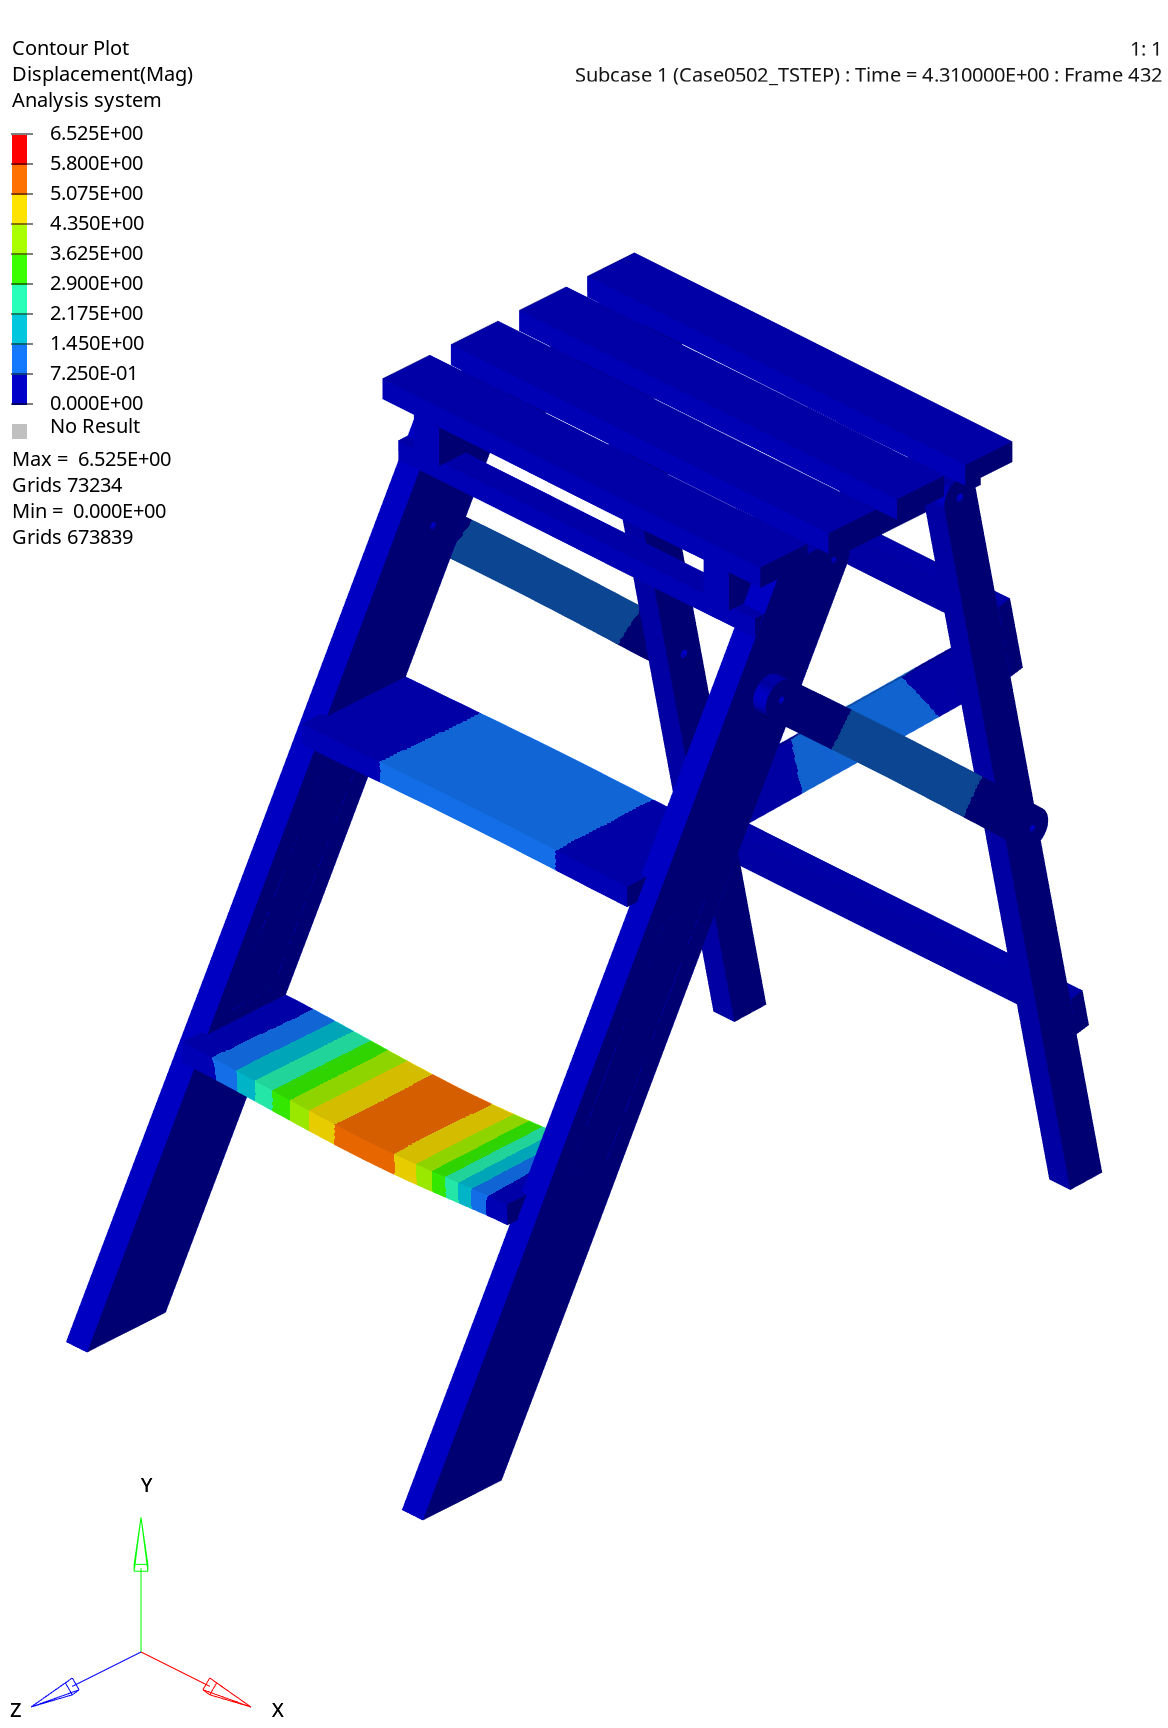
\includegraphics[width=0.32\linewidth]{pics/C020414.png}
    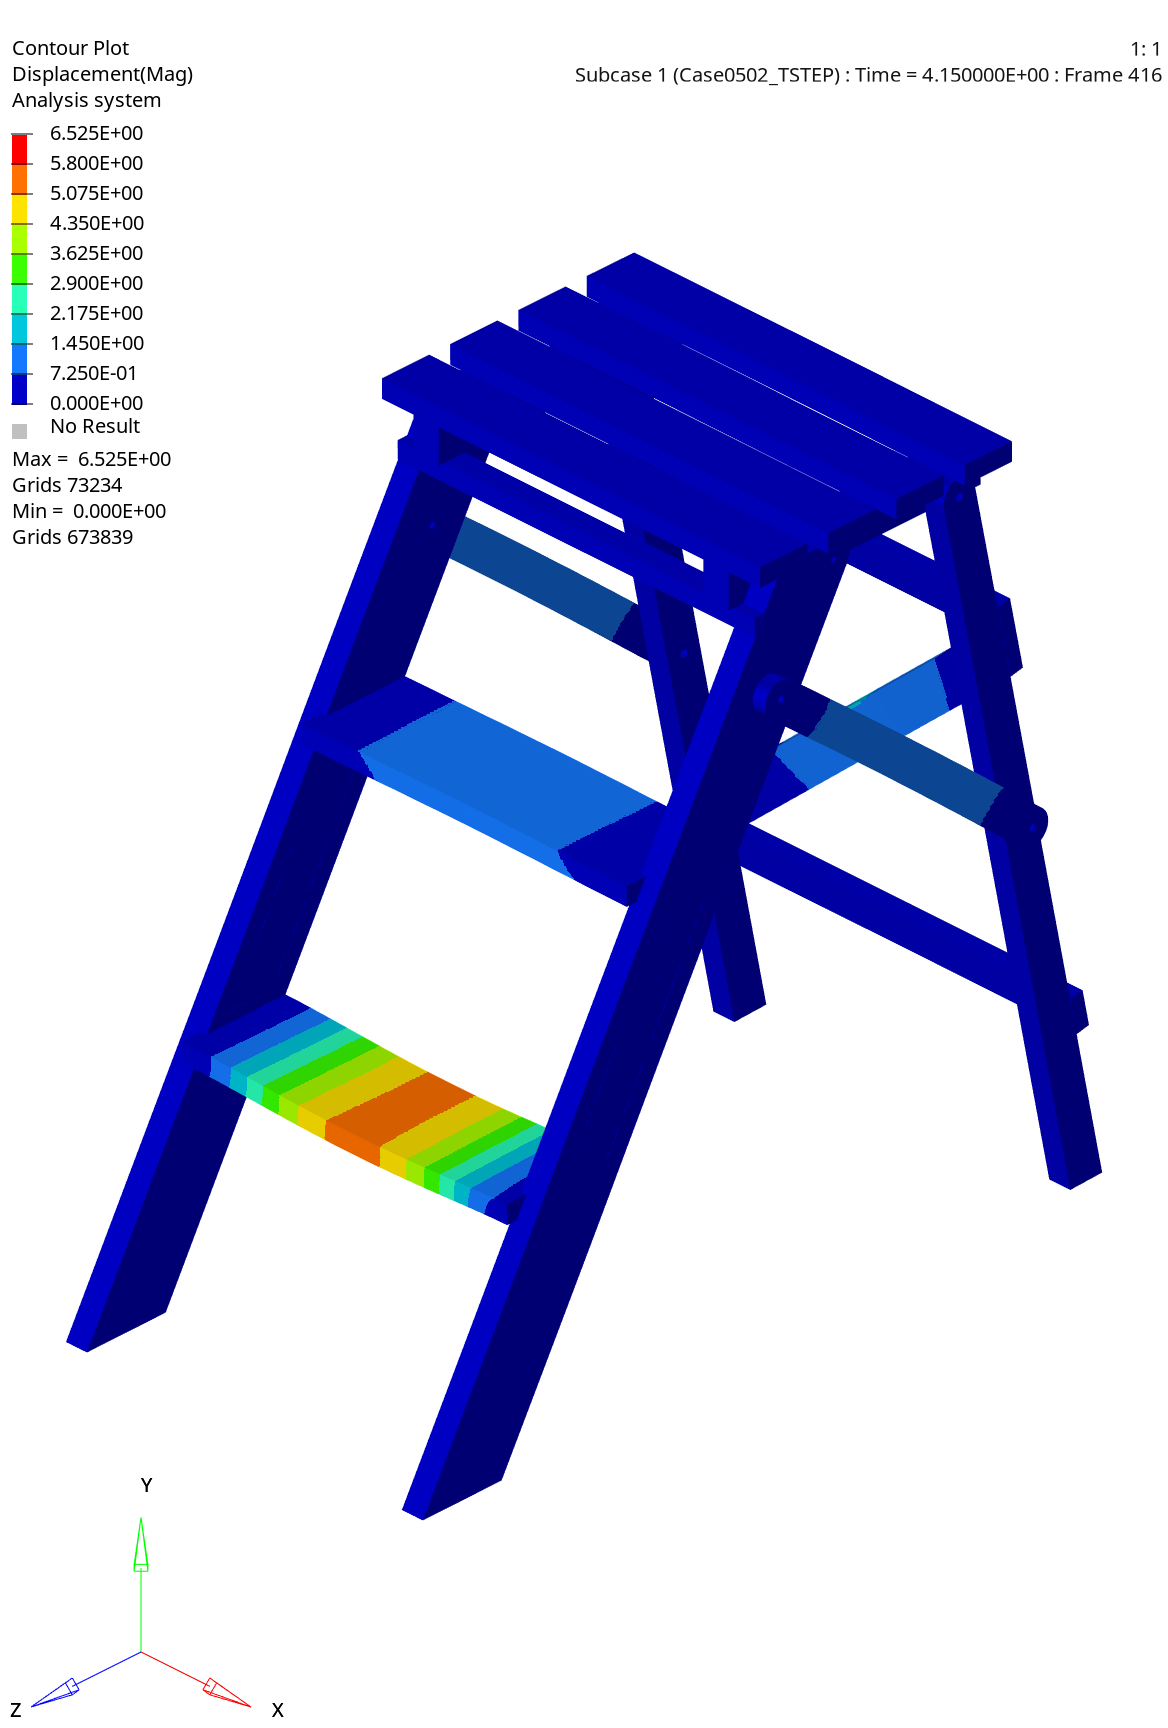
\includegraphics[width=0.32\linewidth]{pics/C020415.png}
    \\
    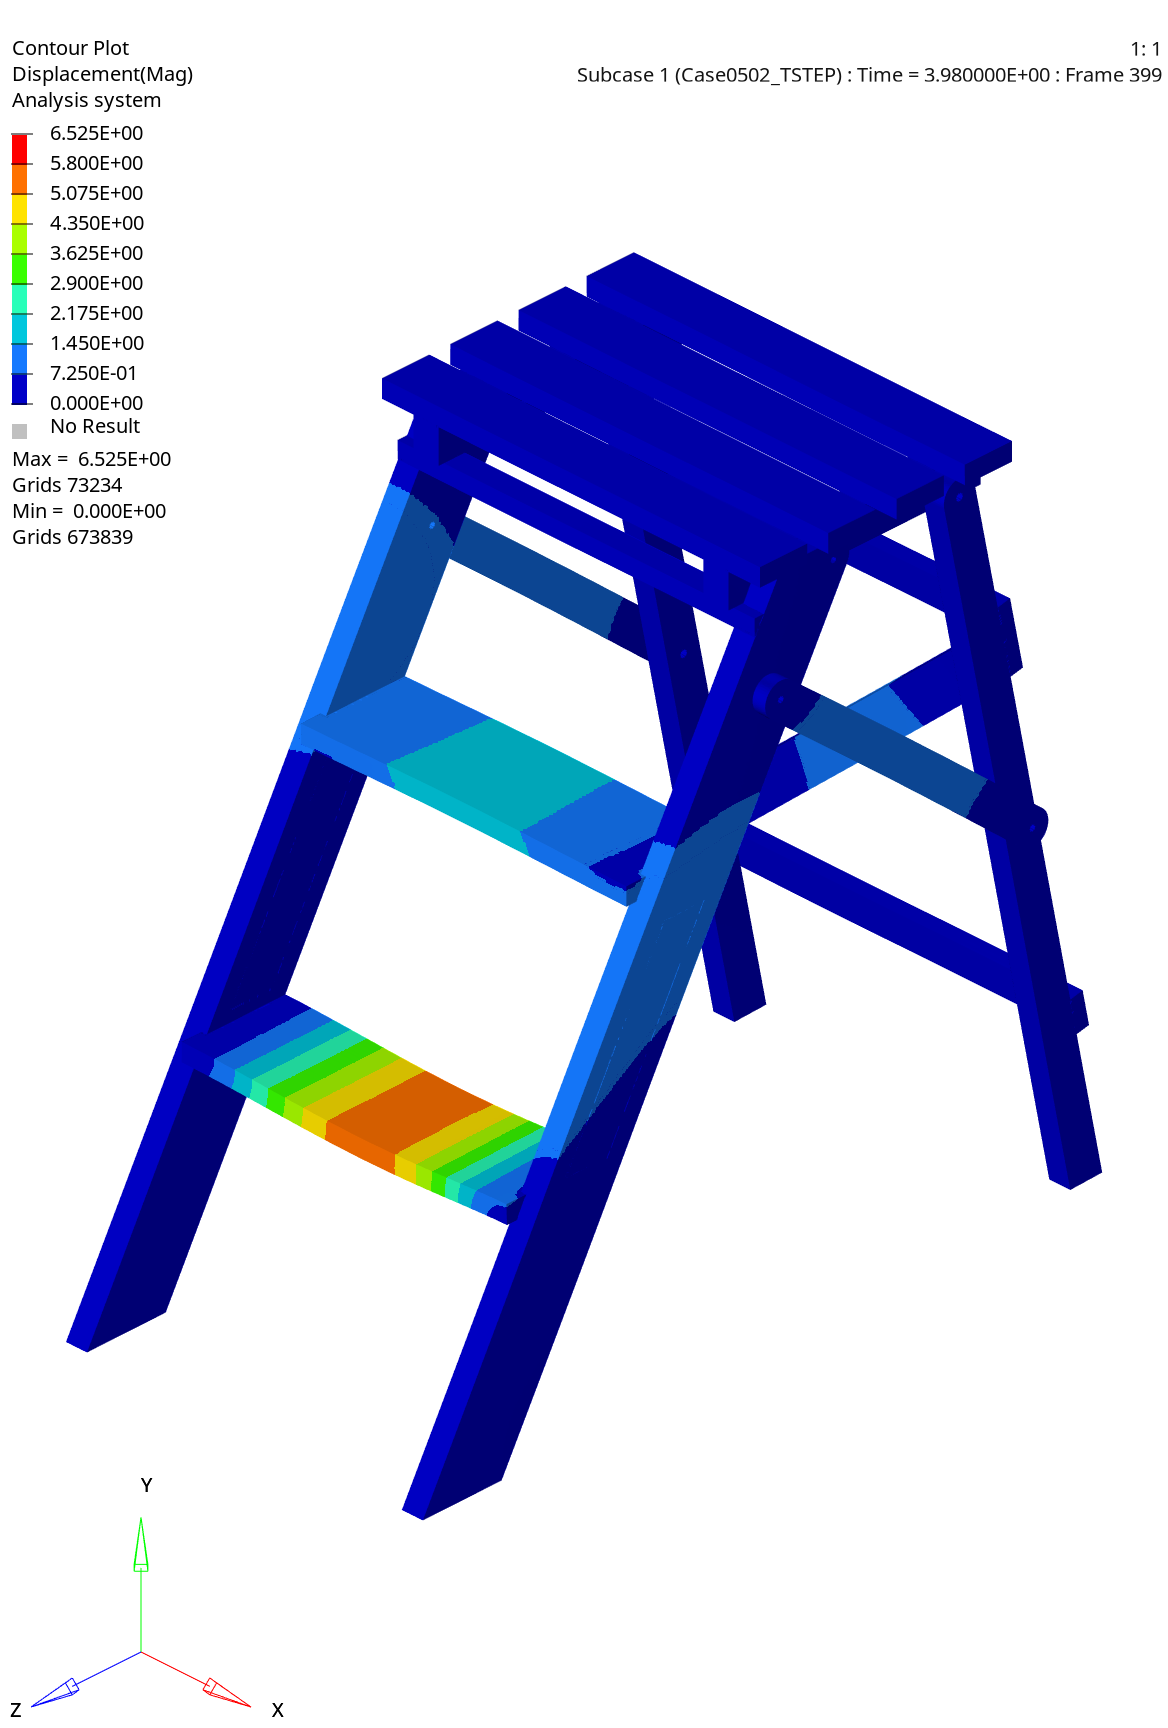
\includegraphics[width=0.32\linewidth]{pics/C020416.png}
    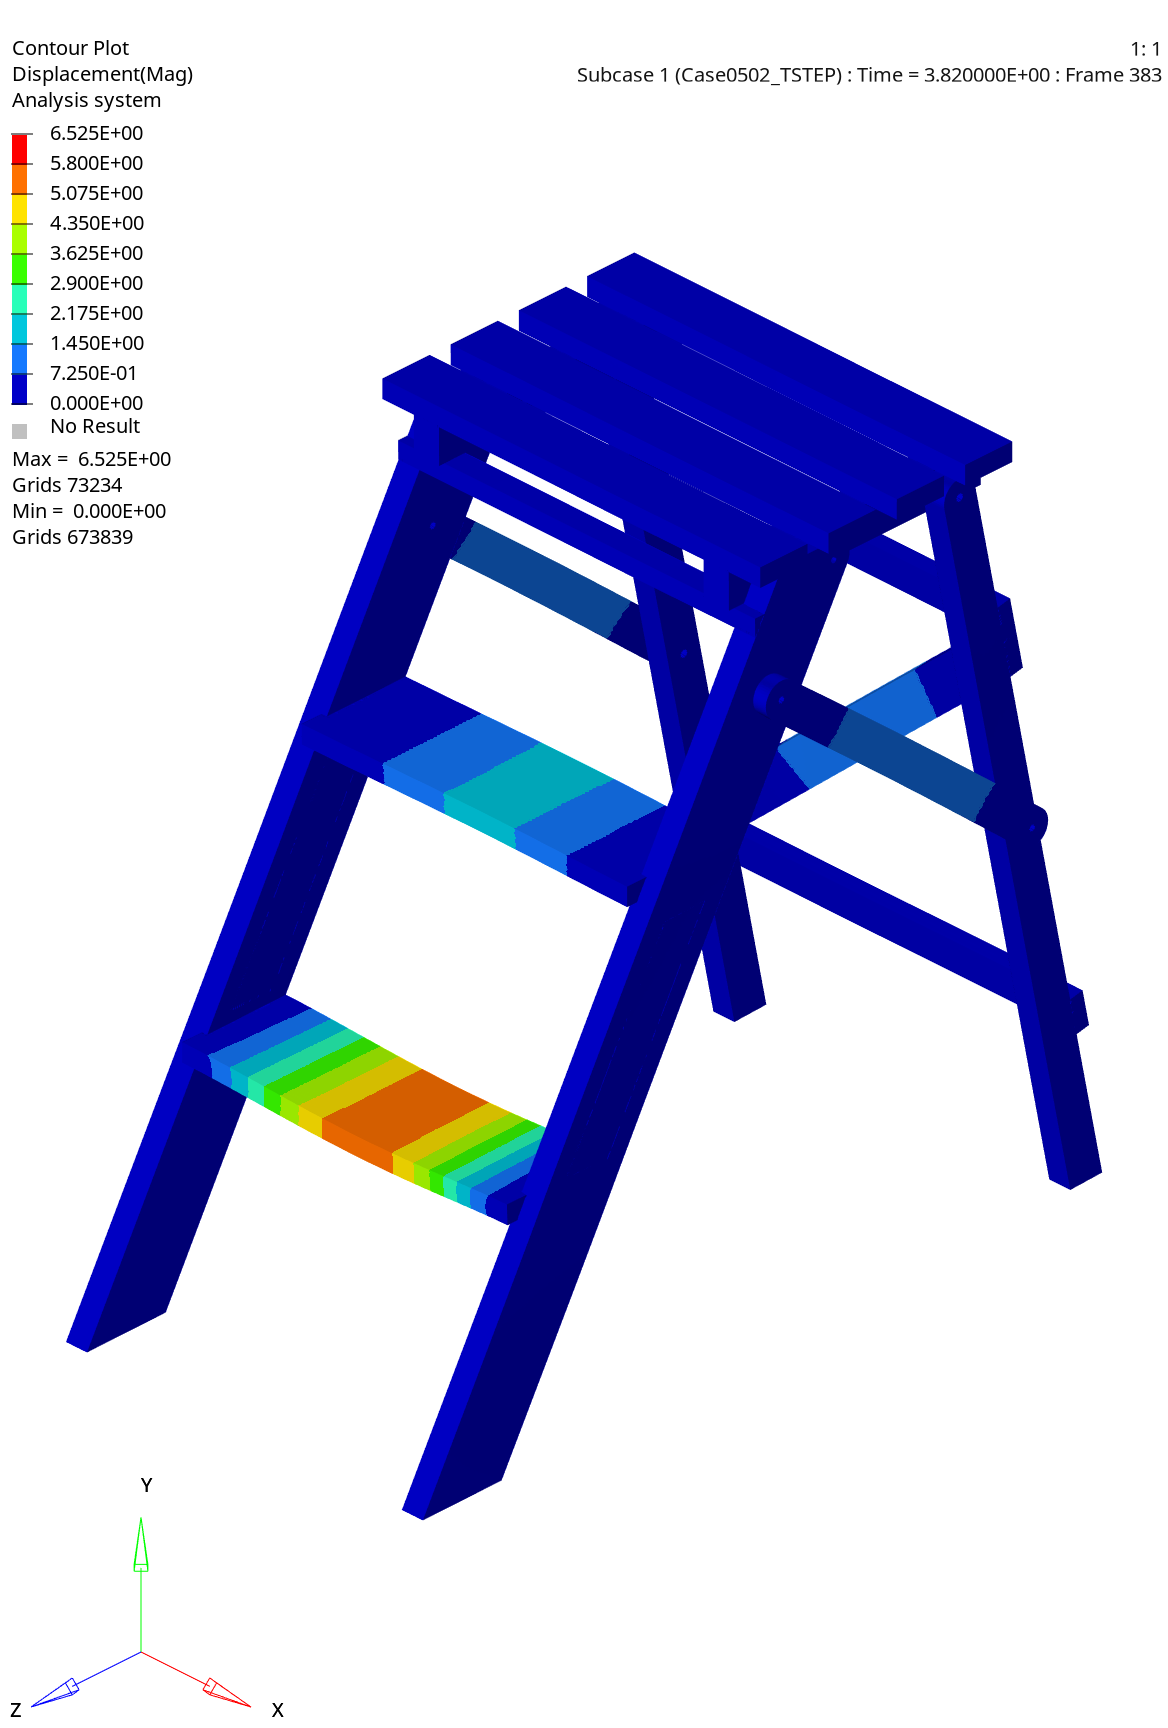
\includegraphics[width=0.32\linewidth]{pics/C020417.png}
    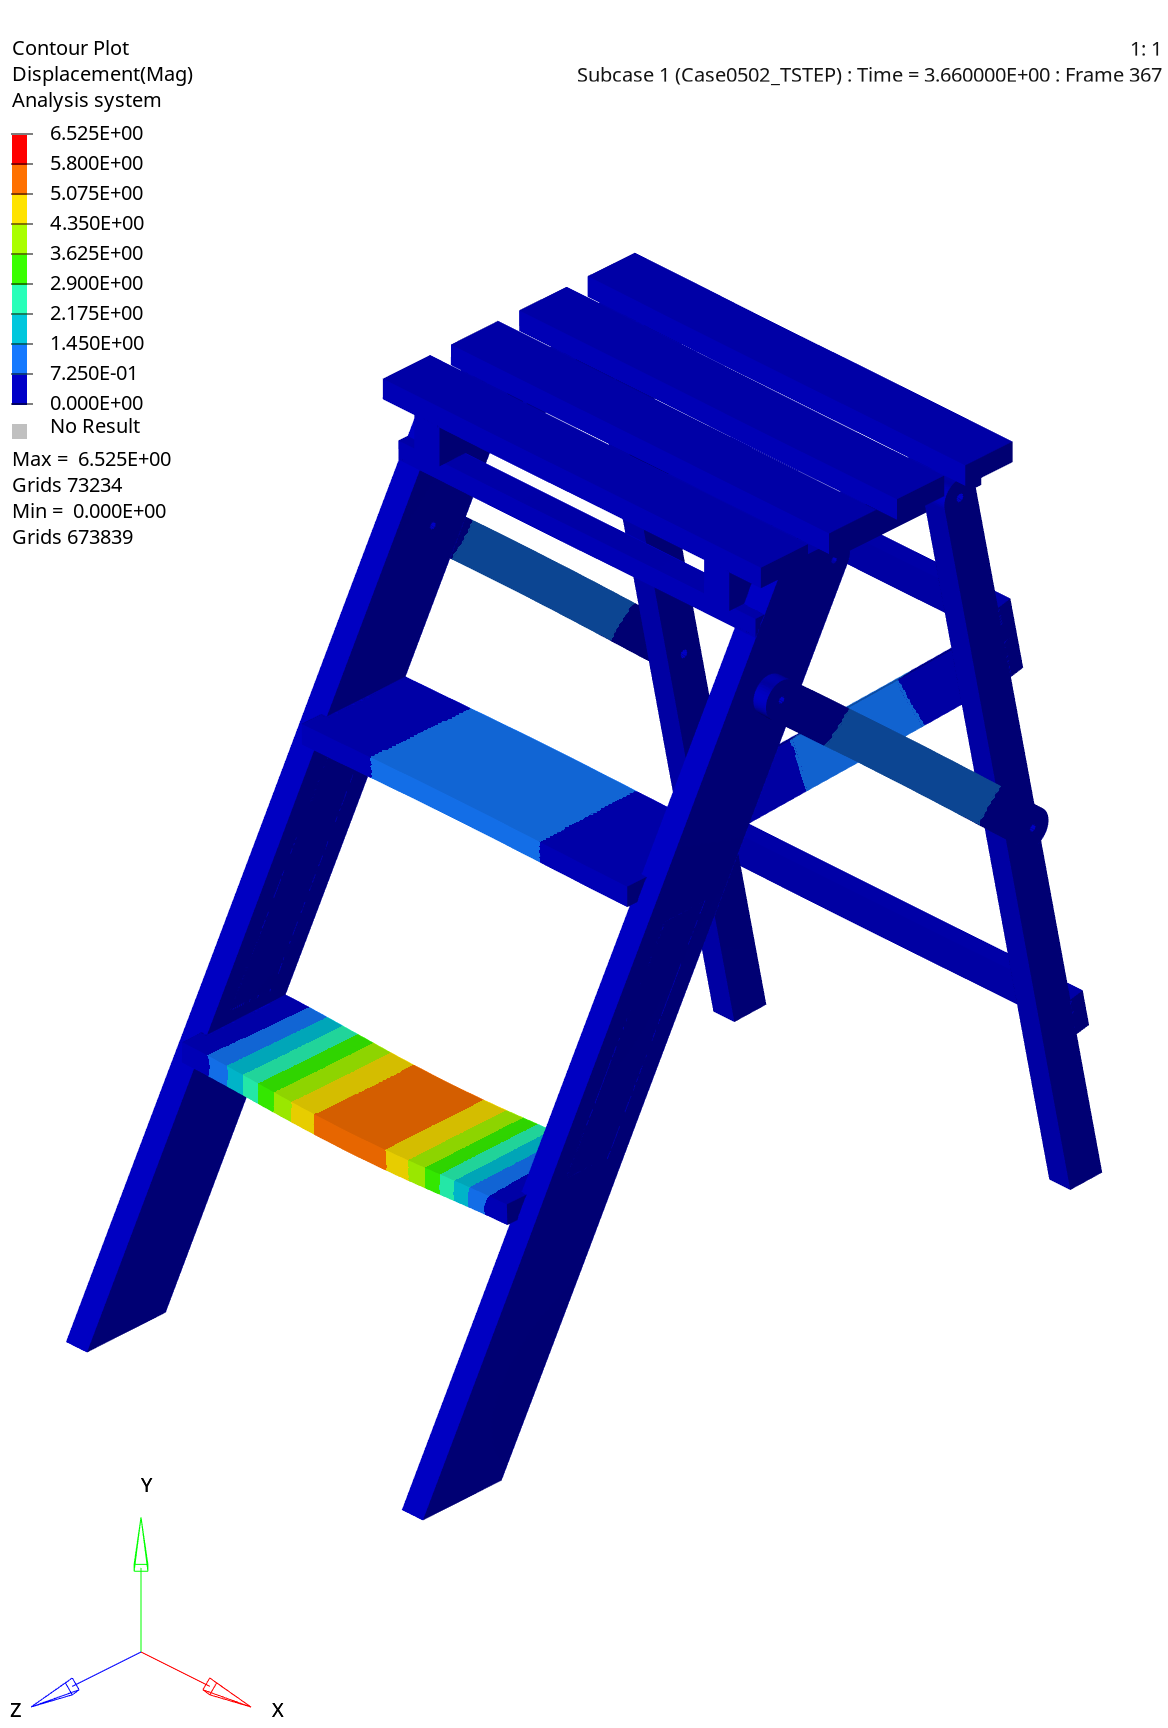
\includegraphics[width=0.32\linewidth]{pics/C020418.png}
    \captionsetup{labelformat=empty}
    \caption{\small{附图2.4.2: 动态特性分析 - 瞬态分析关键点结果输出 - 后9次}}
    \vspace{-0.4cm}
\end{figure}
\newpage{}
\par{}
\begin{figure}[h]
    \centering
    \vspace{-0.1cm}
    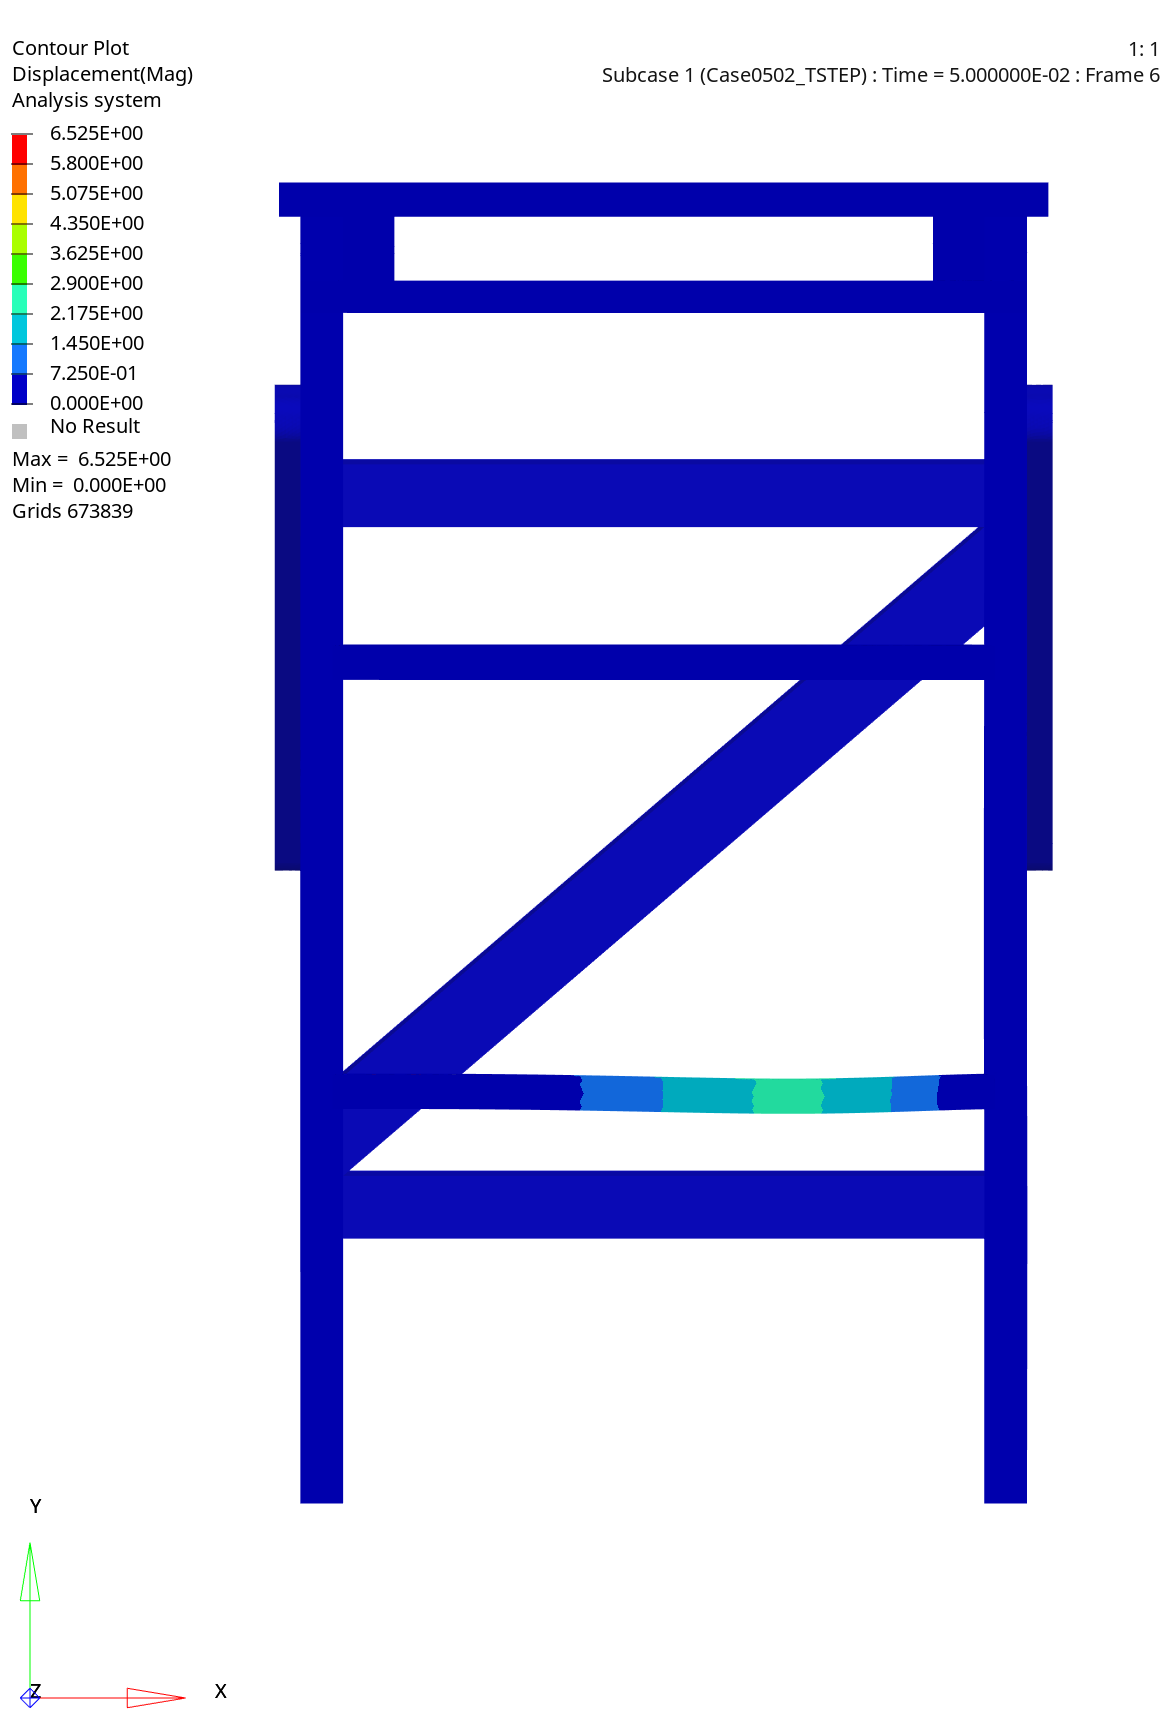
\includegraphics[width=0.48\linewidth]{pics/C020419.png}
    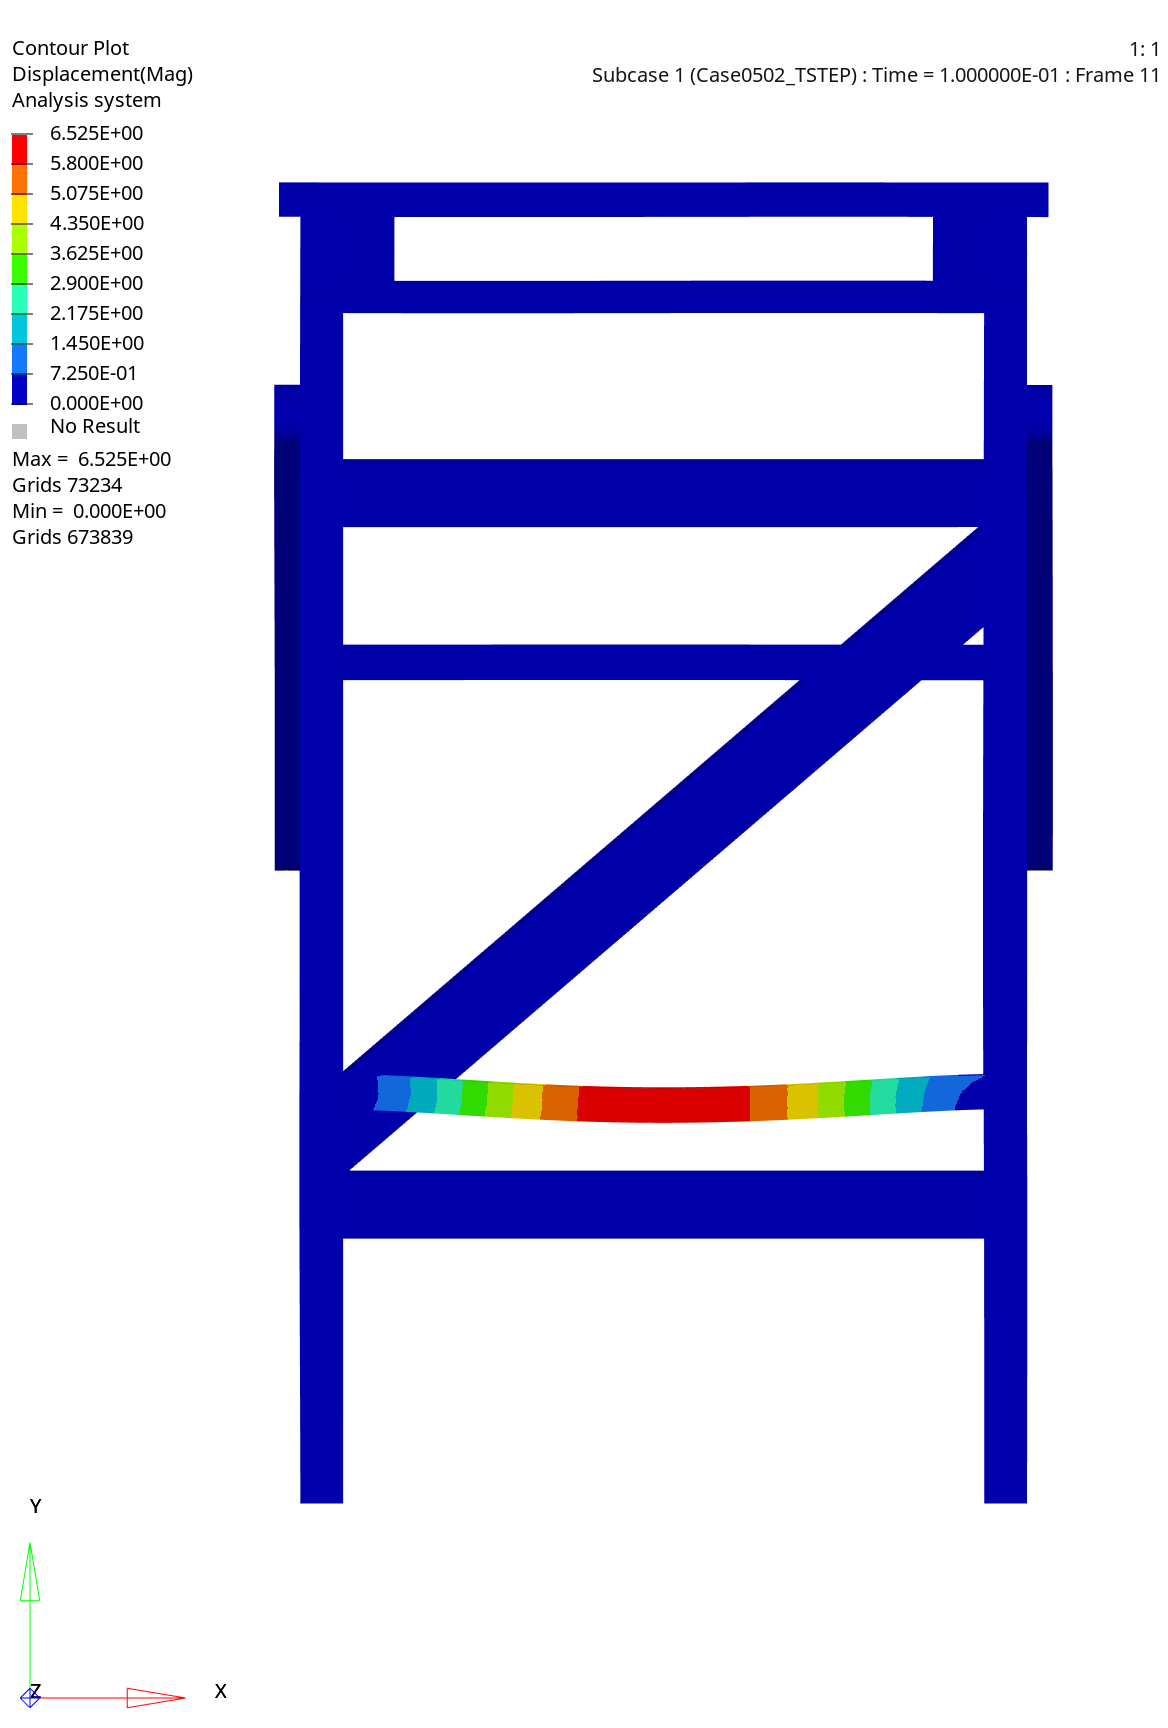
\includegraphics[width=0.48\linewidth]{pics/C020420.png}
    \\
    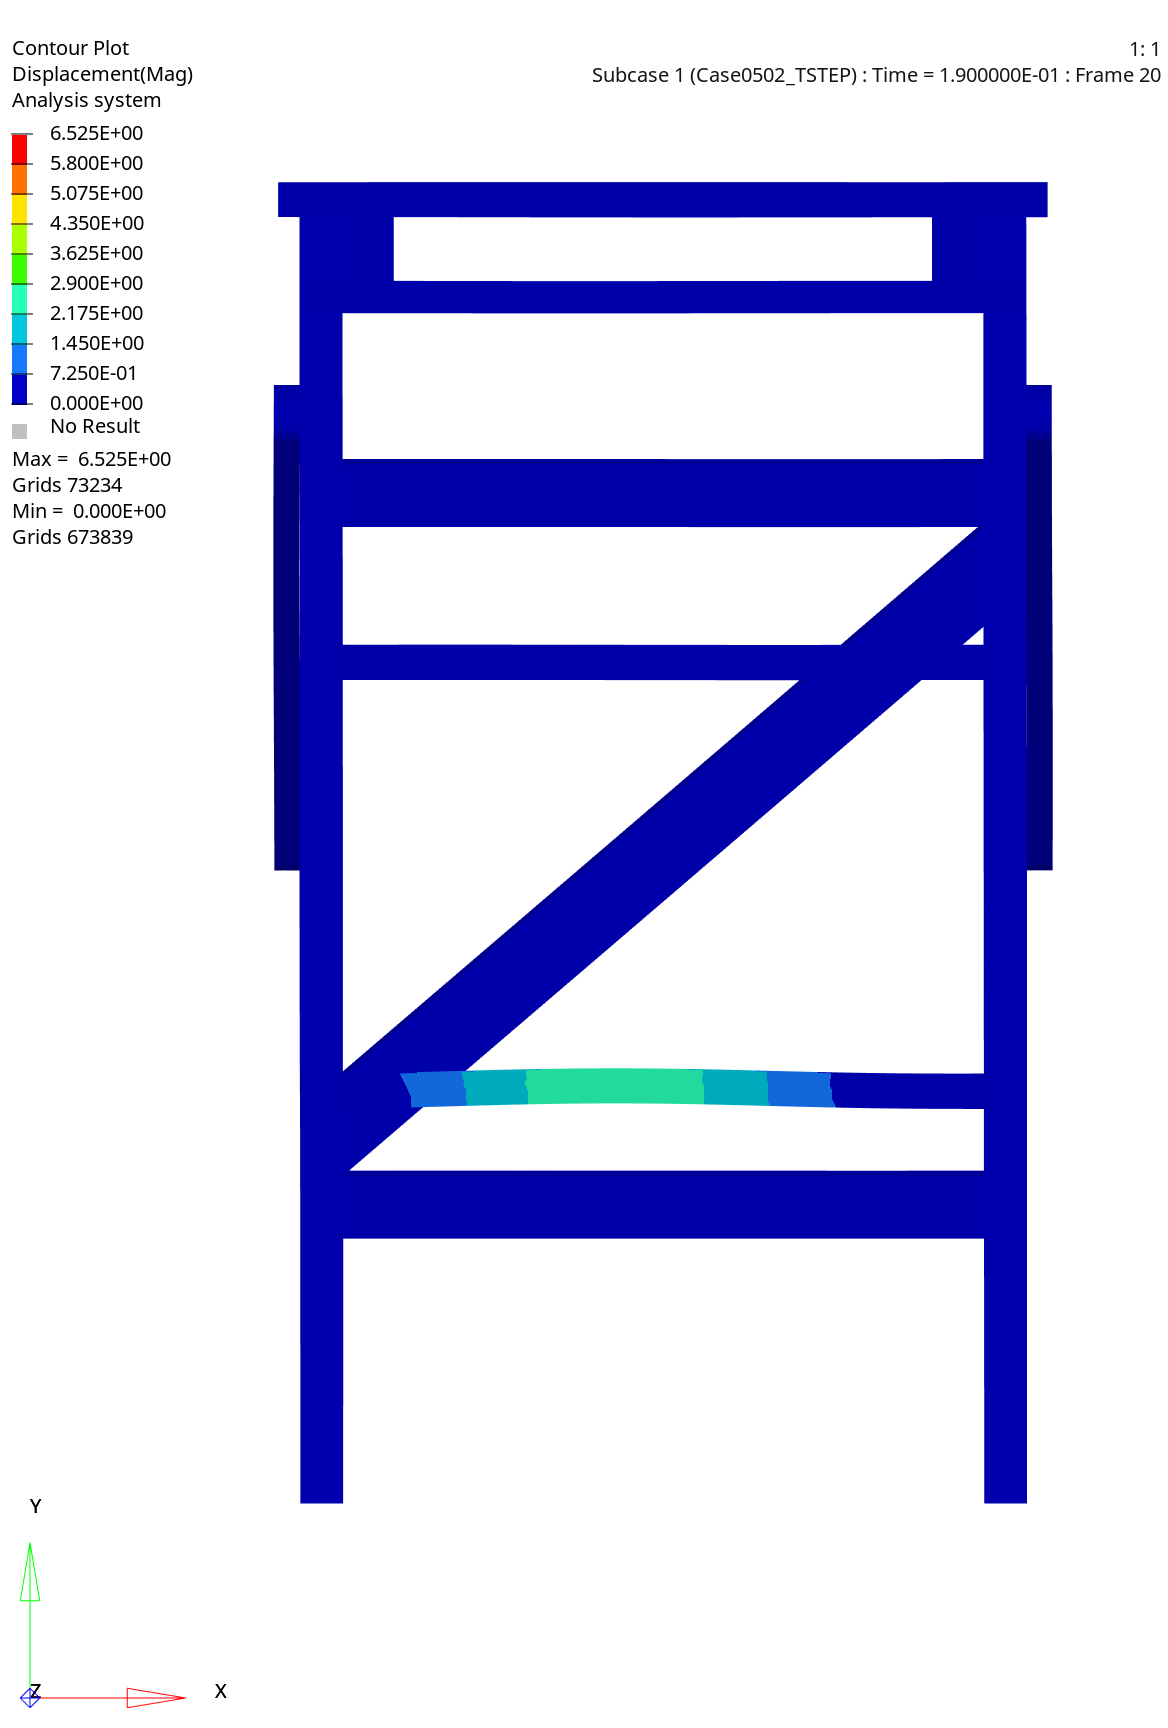
\includegraphics[width=0.48\linewidth]{pics/C020421.png}
    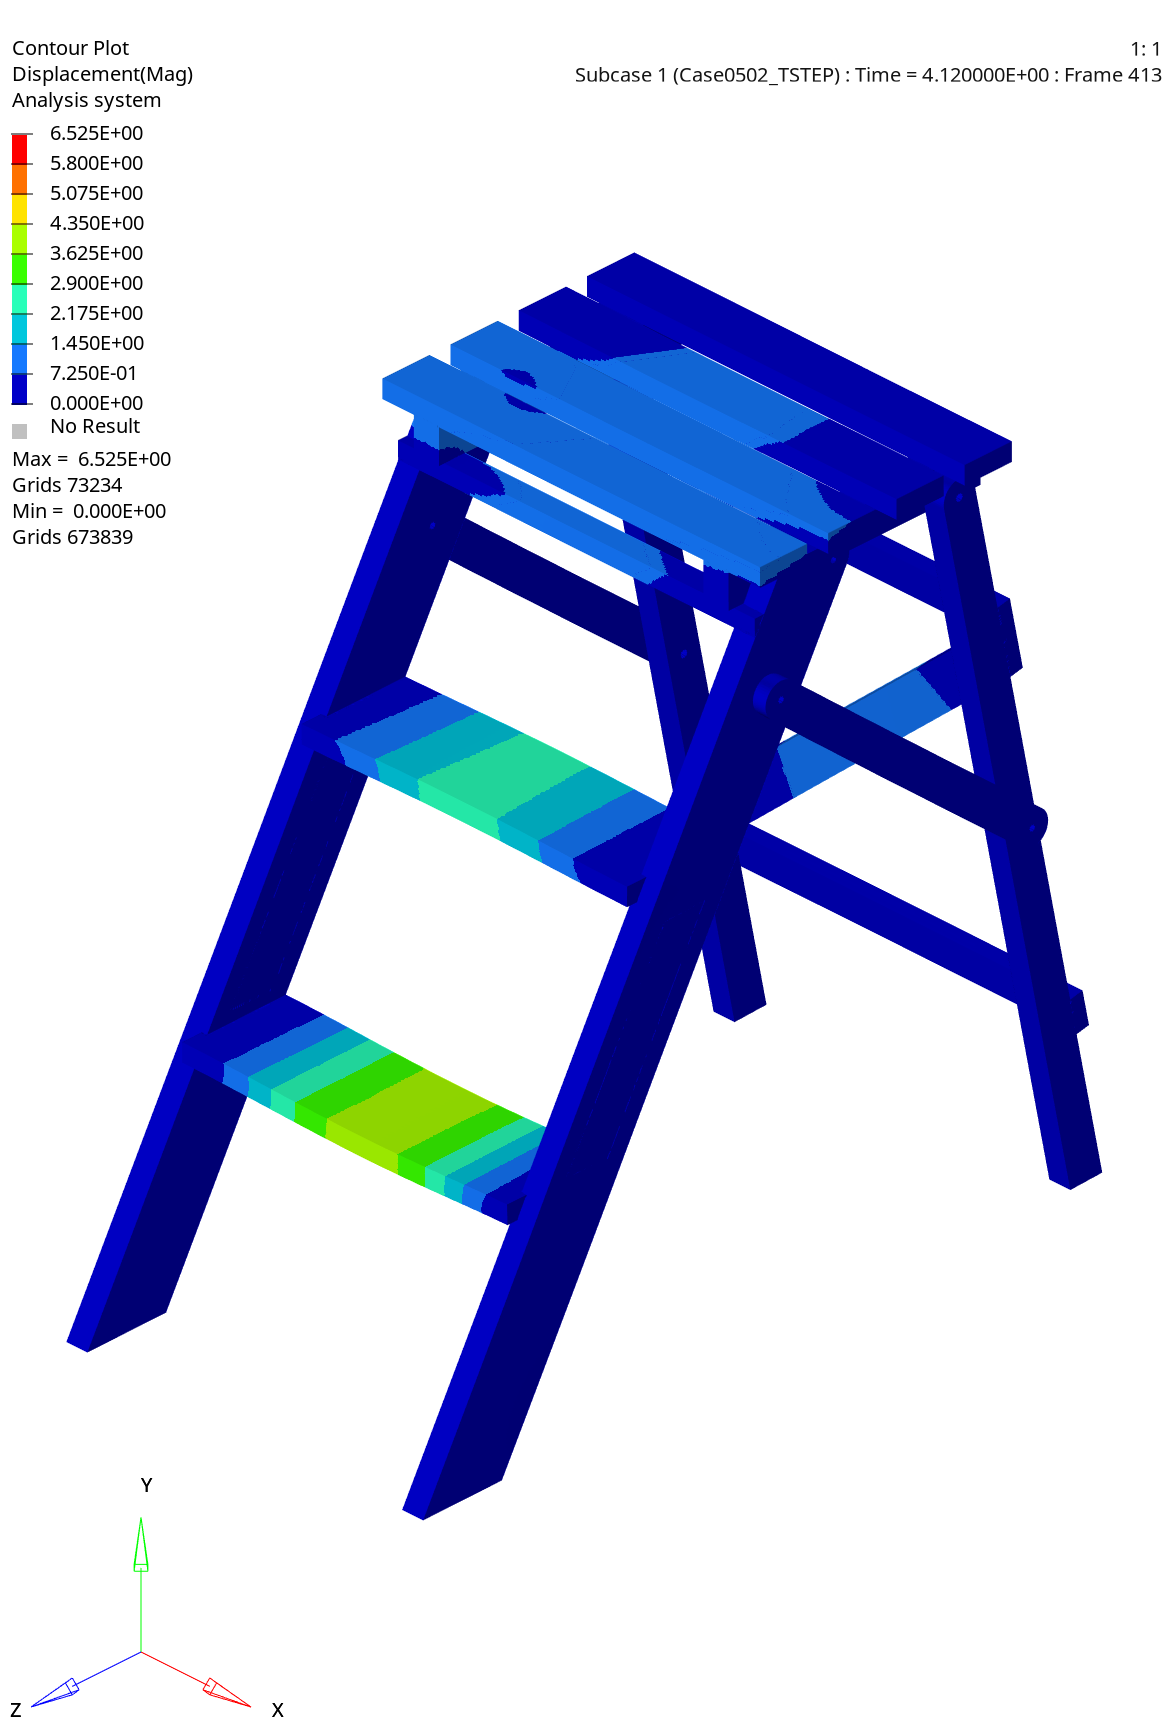
\includegraphics[width=0.48\linewidth]{pics/C020422.png}
    \captionsetup{labelformat=empty}
    \caption{\small{附图2.4.3: 动态特性分析 - 瞬态分析结果输出 - 振动传递}}
    \vspace{-0.4cm}
\end{figure}
\newpage{}
\par{}
\begin{figure}[h]
    \centering
    \vspace{-0.1cm}
    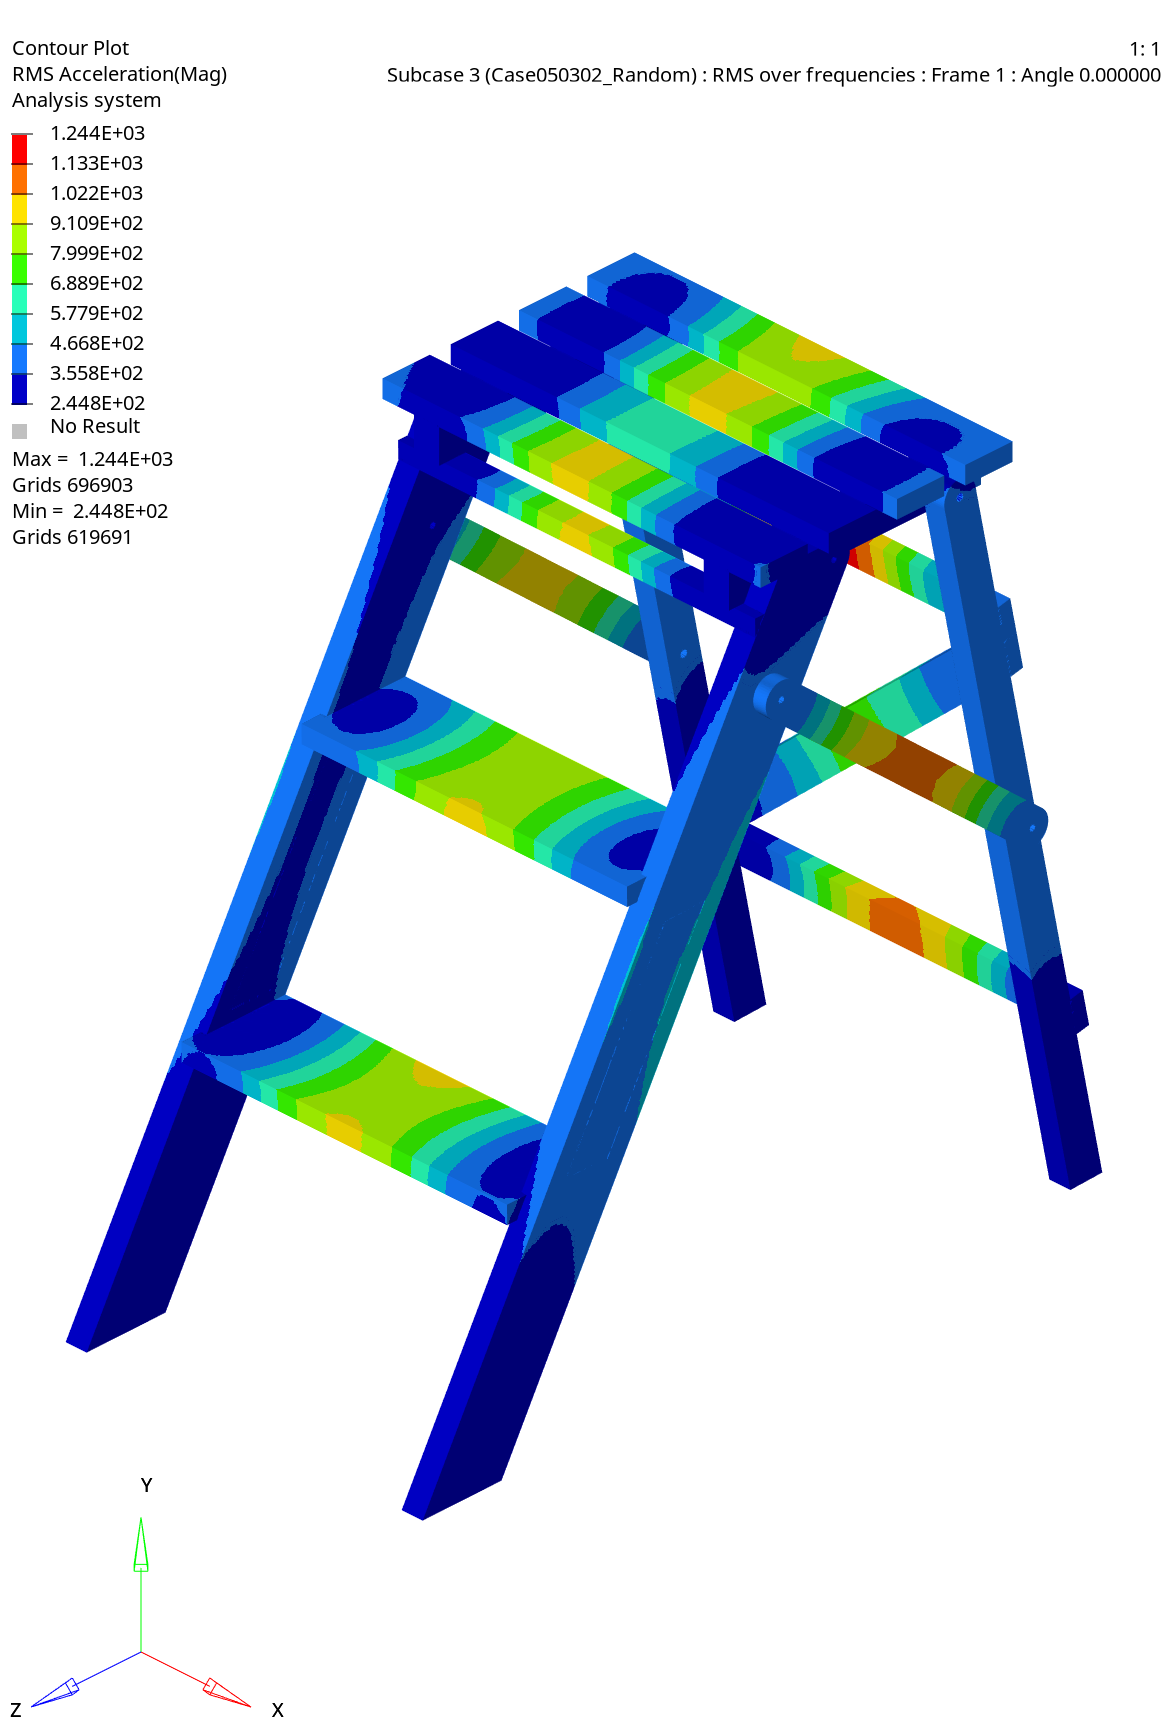
\includegraphics[width=0.48\linewidth]{pics/C020501.png}
    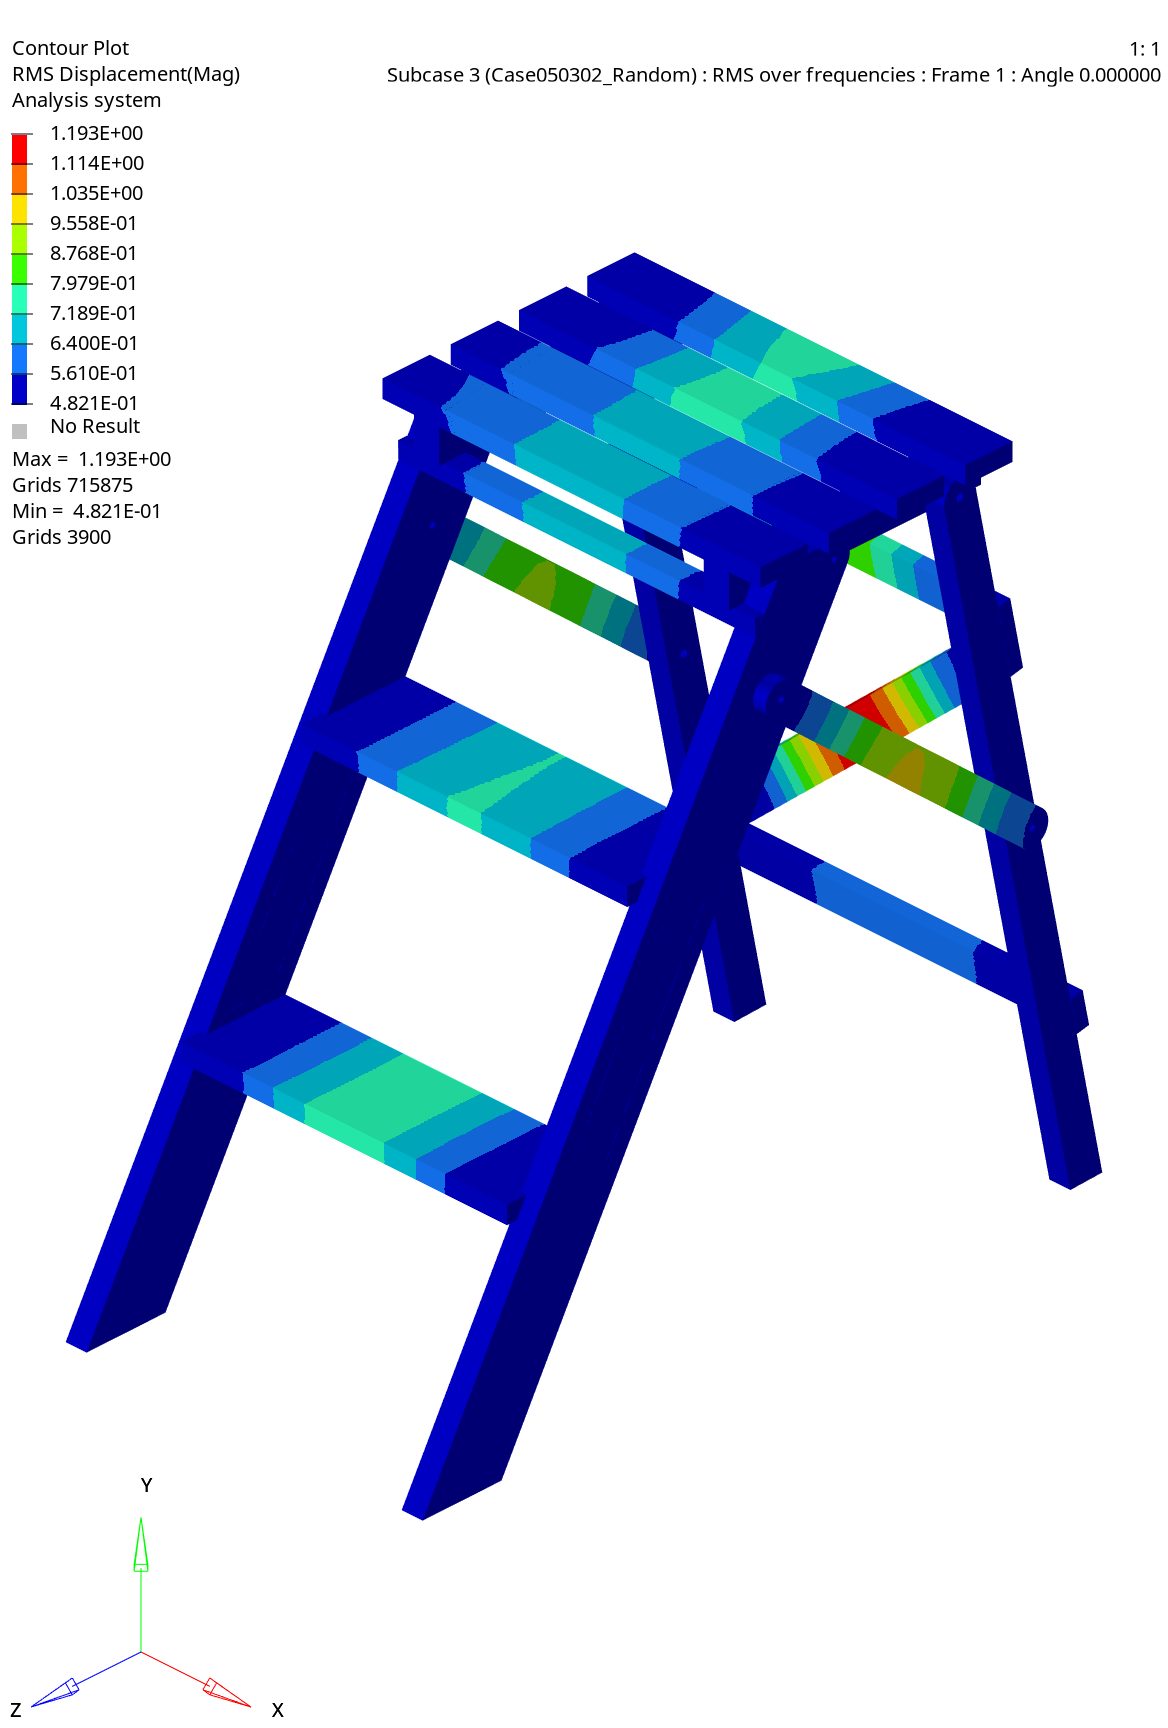
\includegraphics[width=0.48\linewidth]{pics/C020502.png}
    \\
    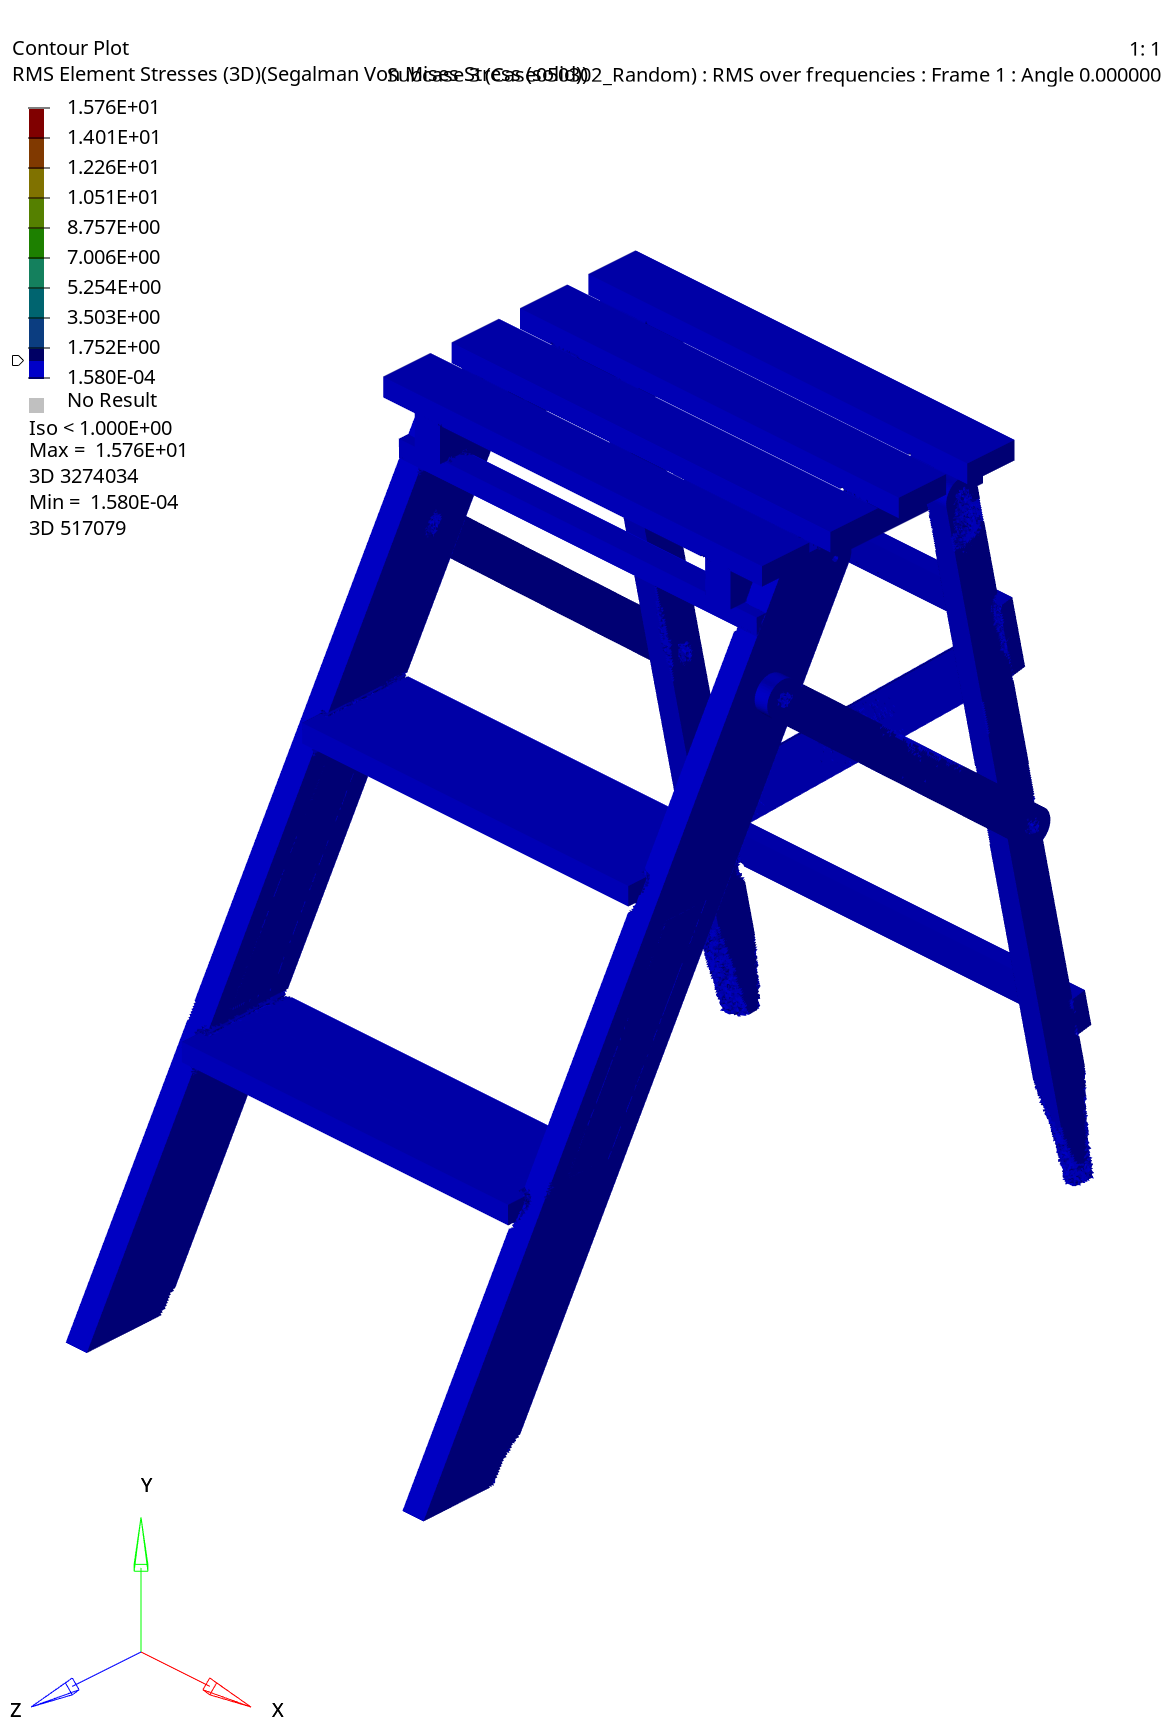
\includegraphics[width=0.48\linewidth]{pics/C020503.png}
    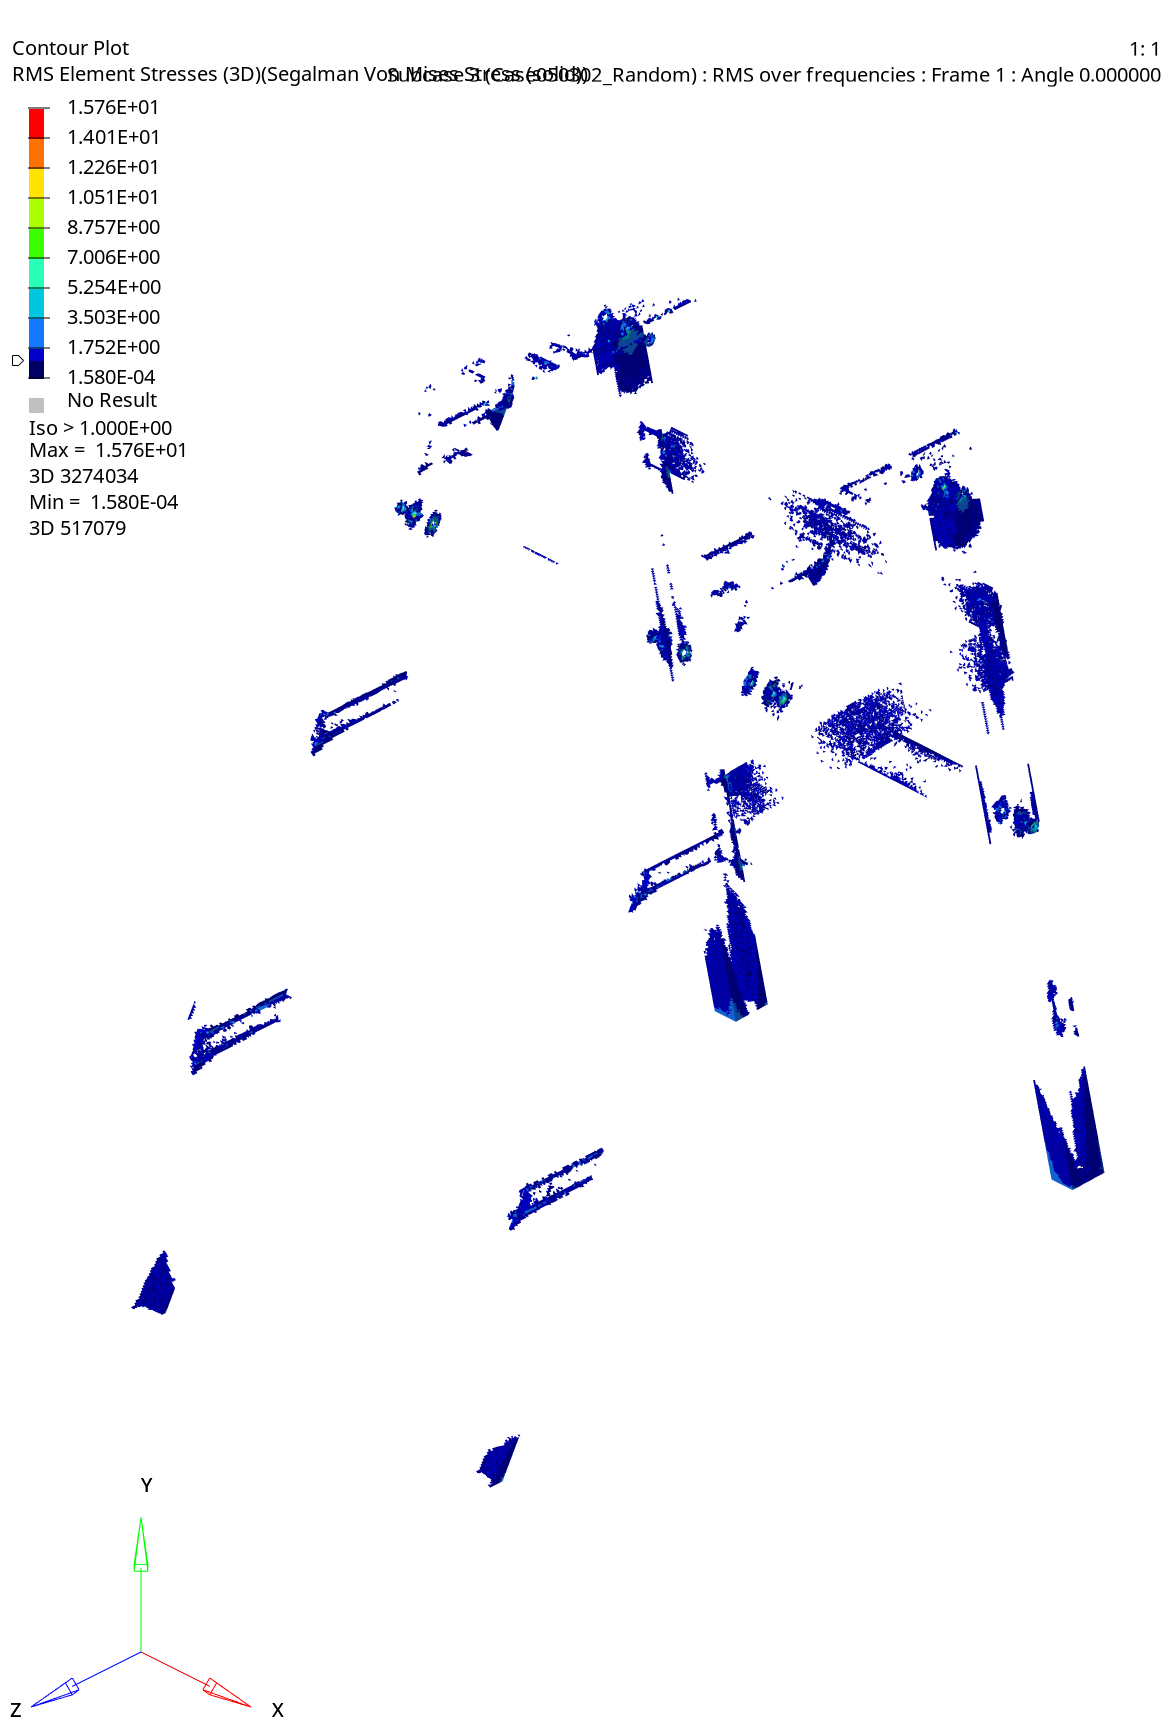
\includegraphics[width=0.48\linewidth]{pics/C020504.png}
    \captionsetup{labelformat=empty}
    \caption{\small{附图2.5: 动态特性分析 - 随机振动分析结果输出}}
    \vspace{-0.4cm}
\end{figure}
\newpage{}
\par{}
\begin{figure}[h]
    \centering
    \vspace{-0.1cm}
    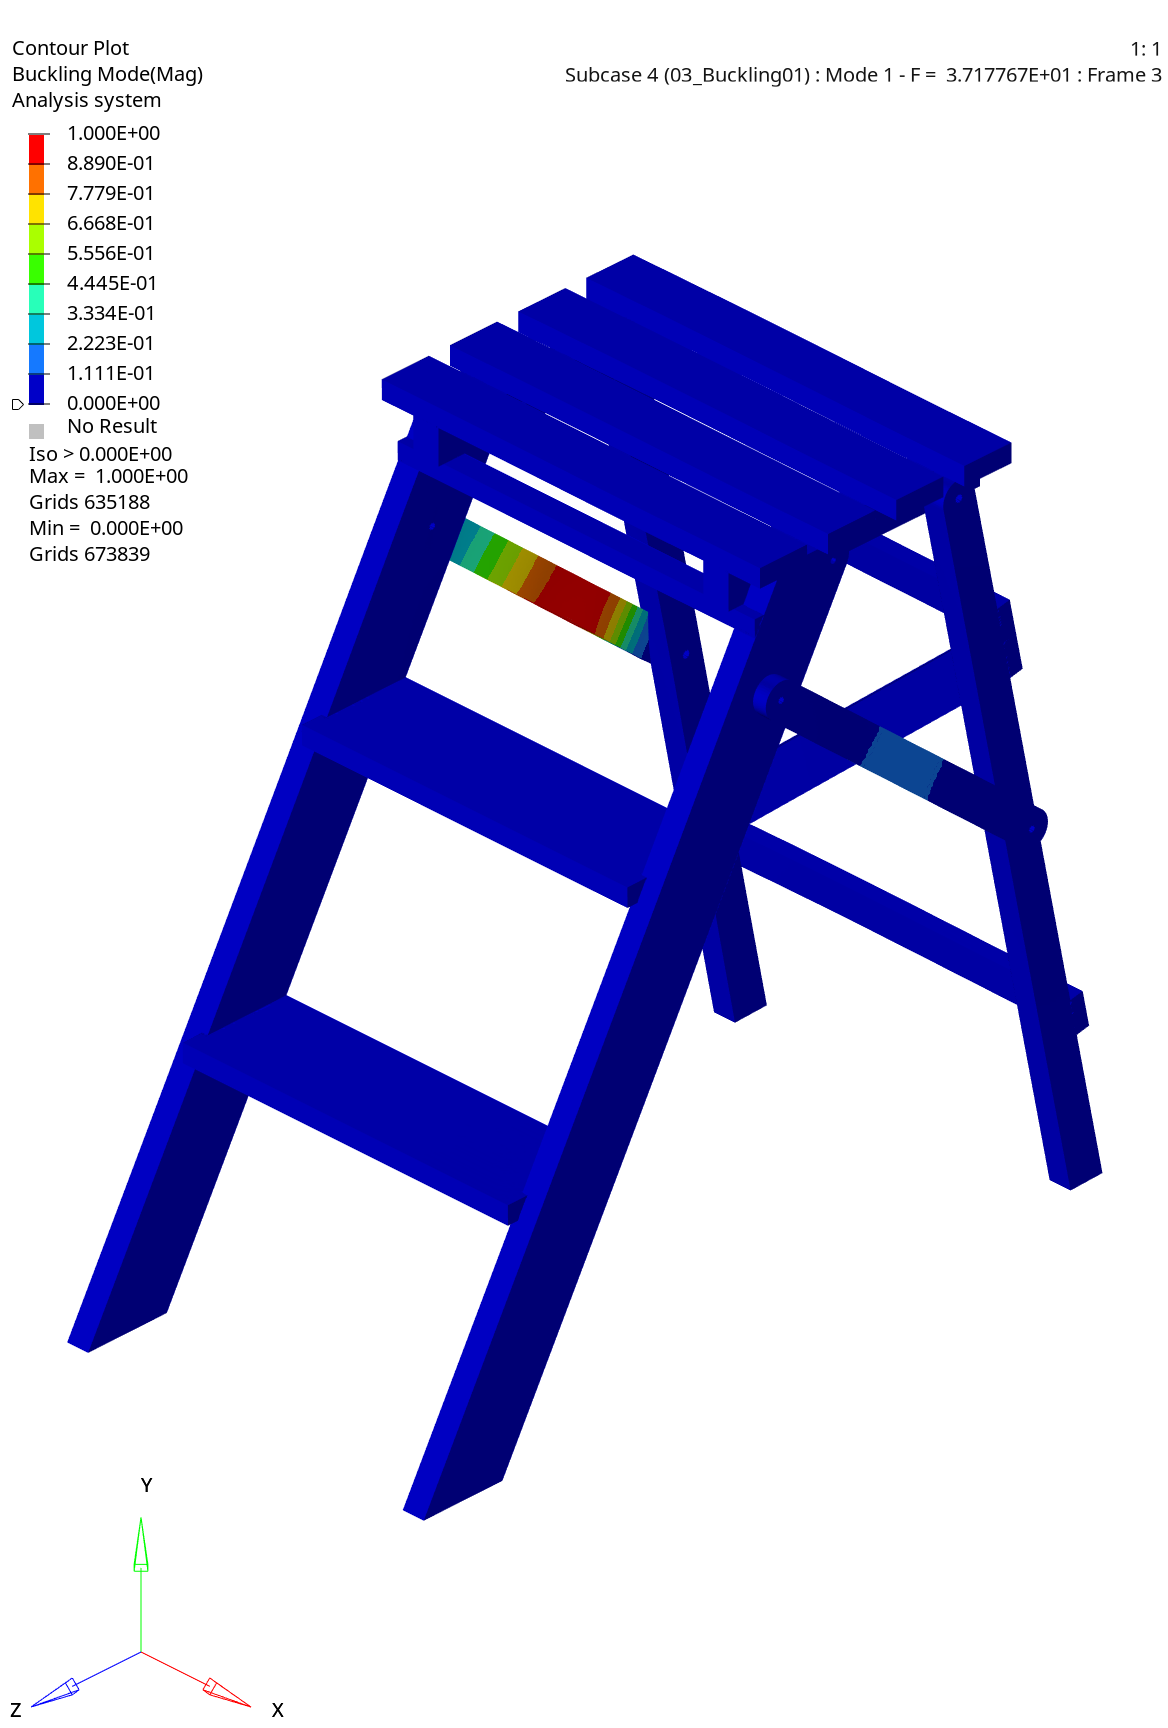
\includegraphics[width=0.48\linewidth]{pics/C030101.png}
    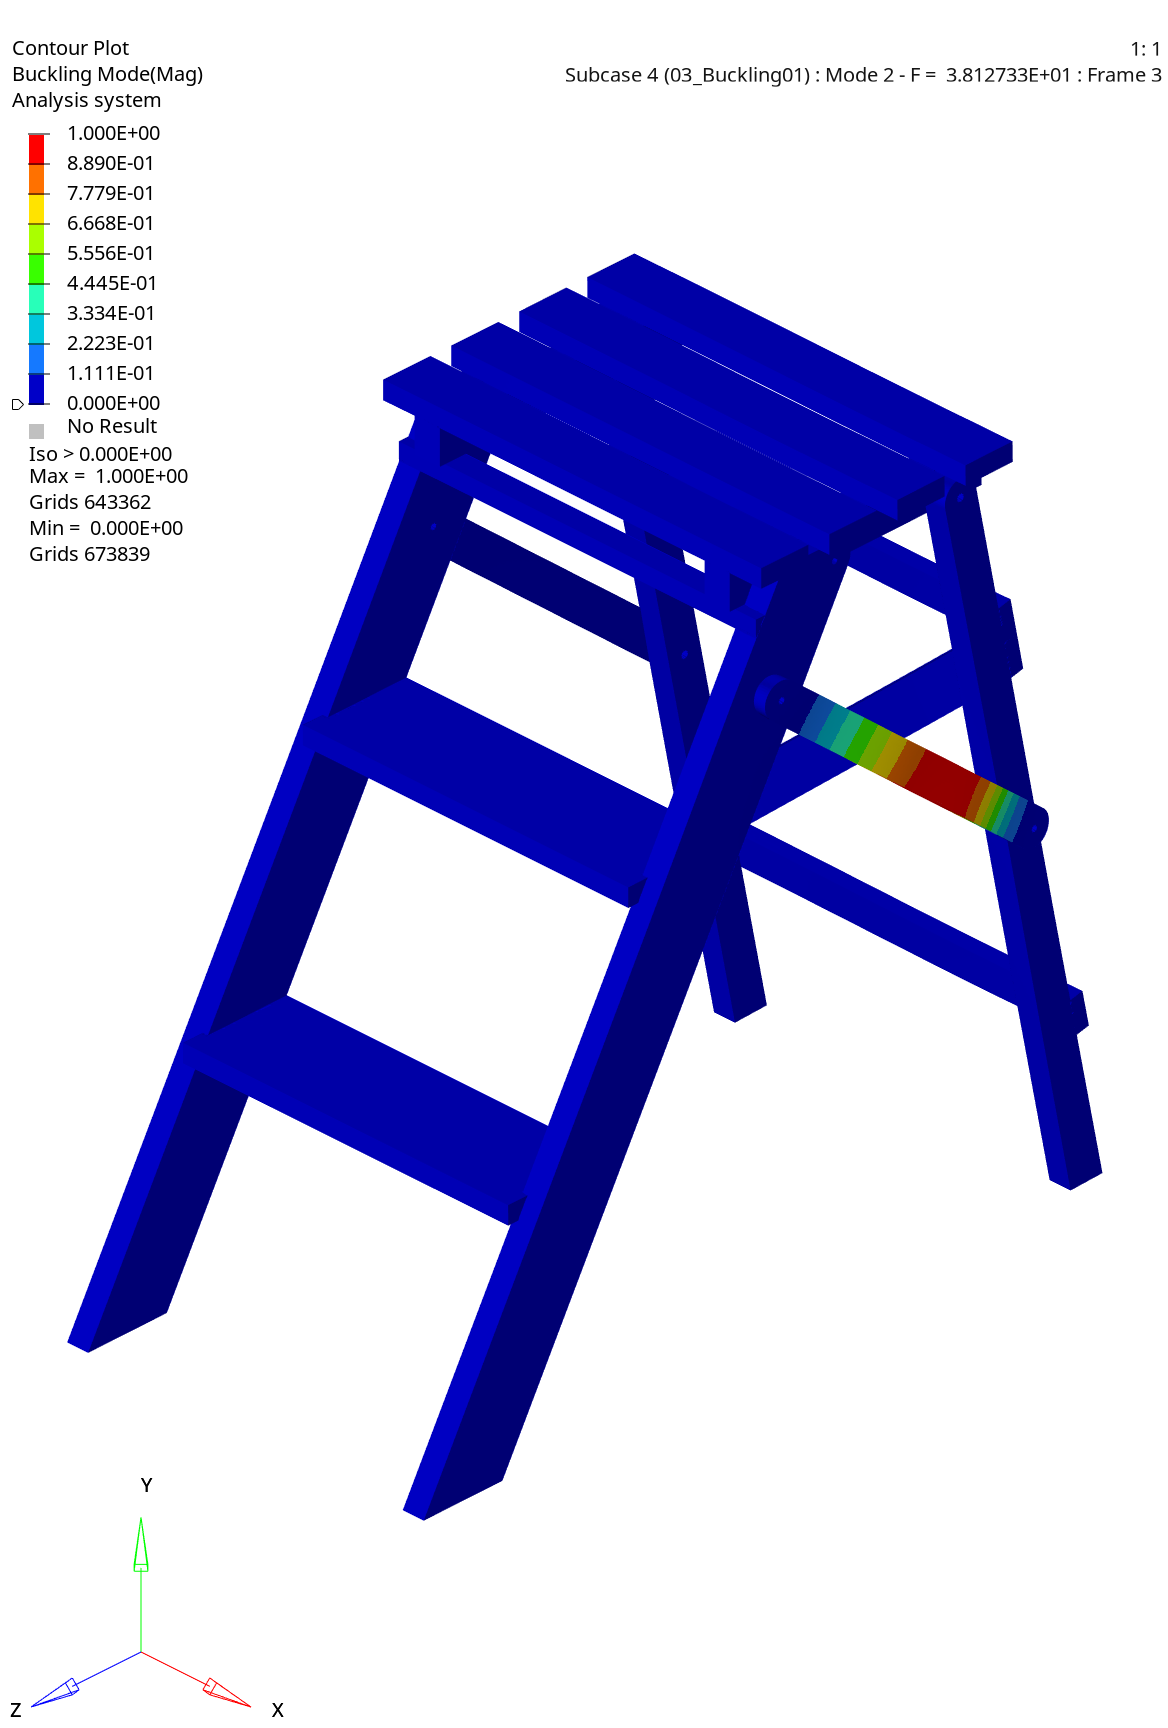
\includegraphics[width=0.48\linewidth]{pics/C030102.png}
    \\
    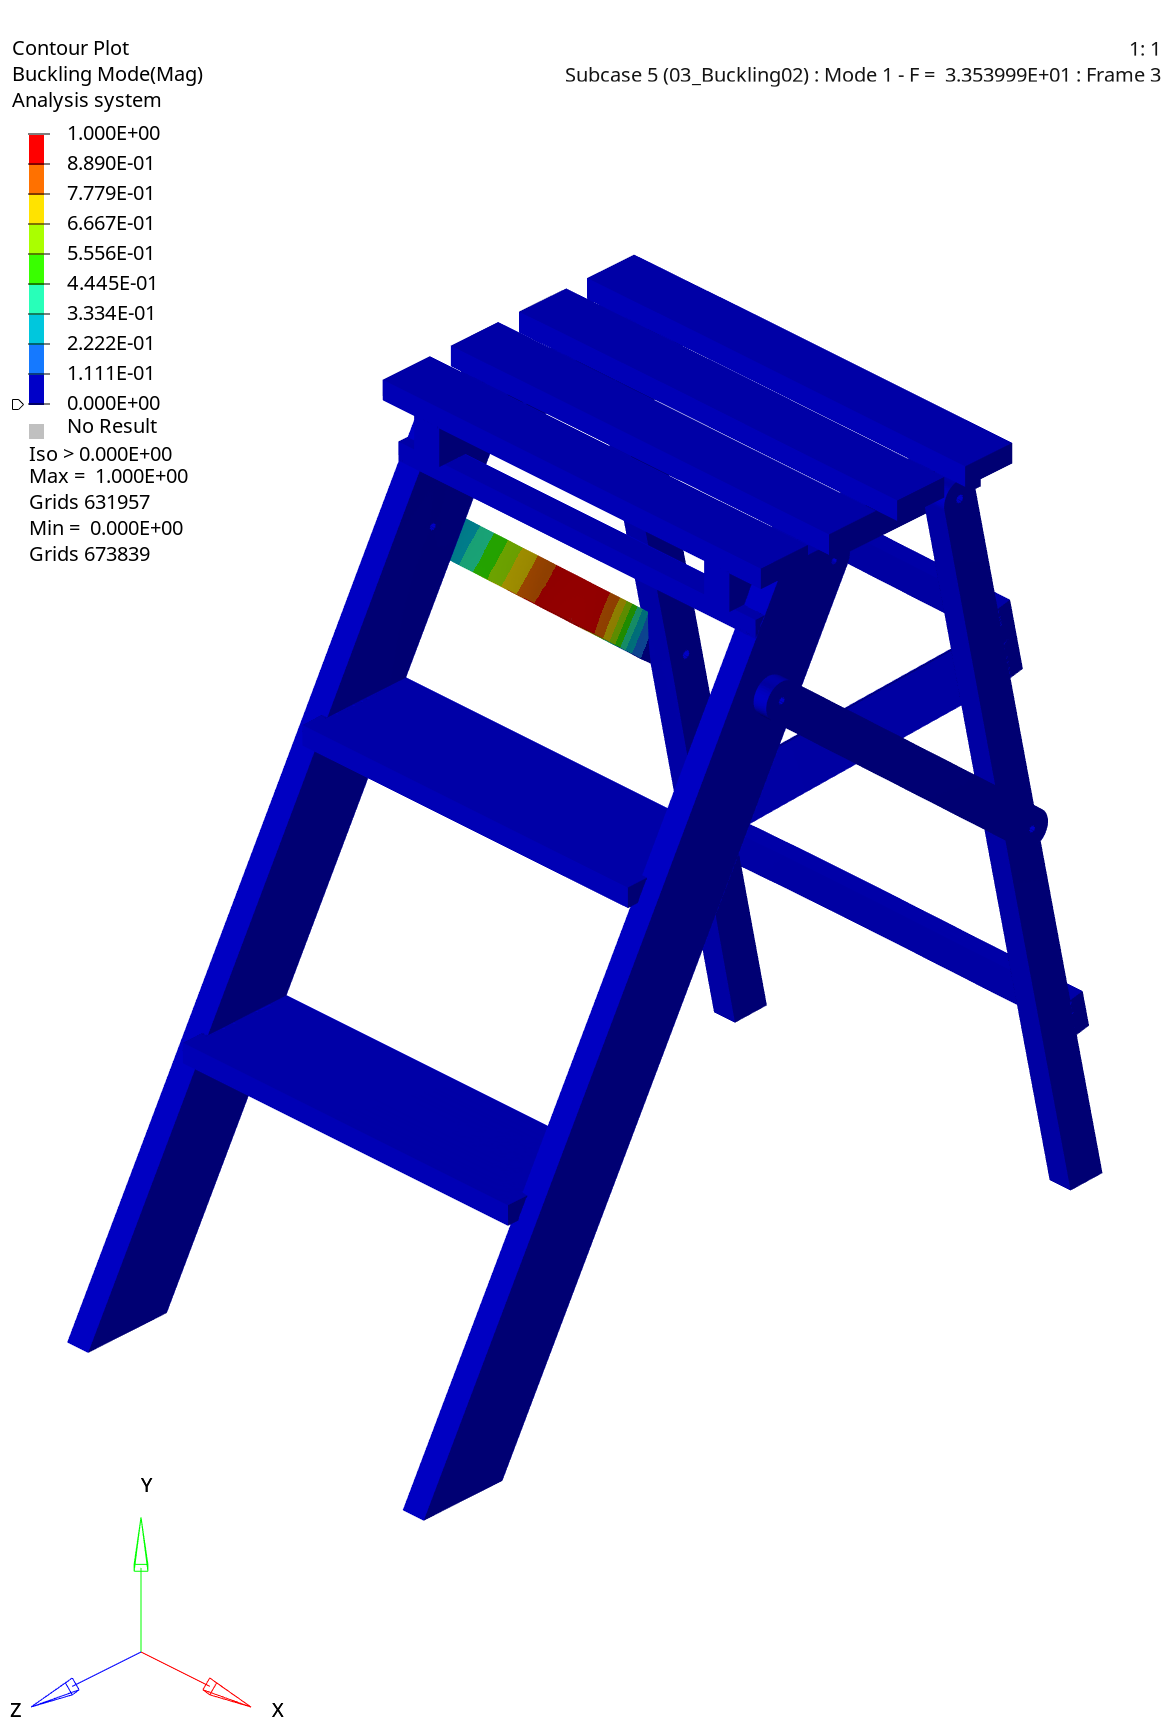
\includegraphics[width=0.48\linewidth]{pics/C030103.png}
    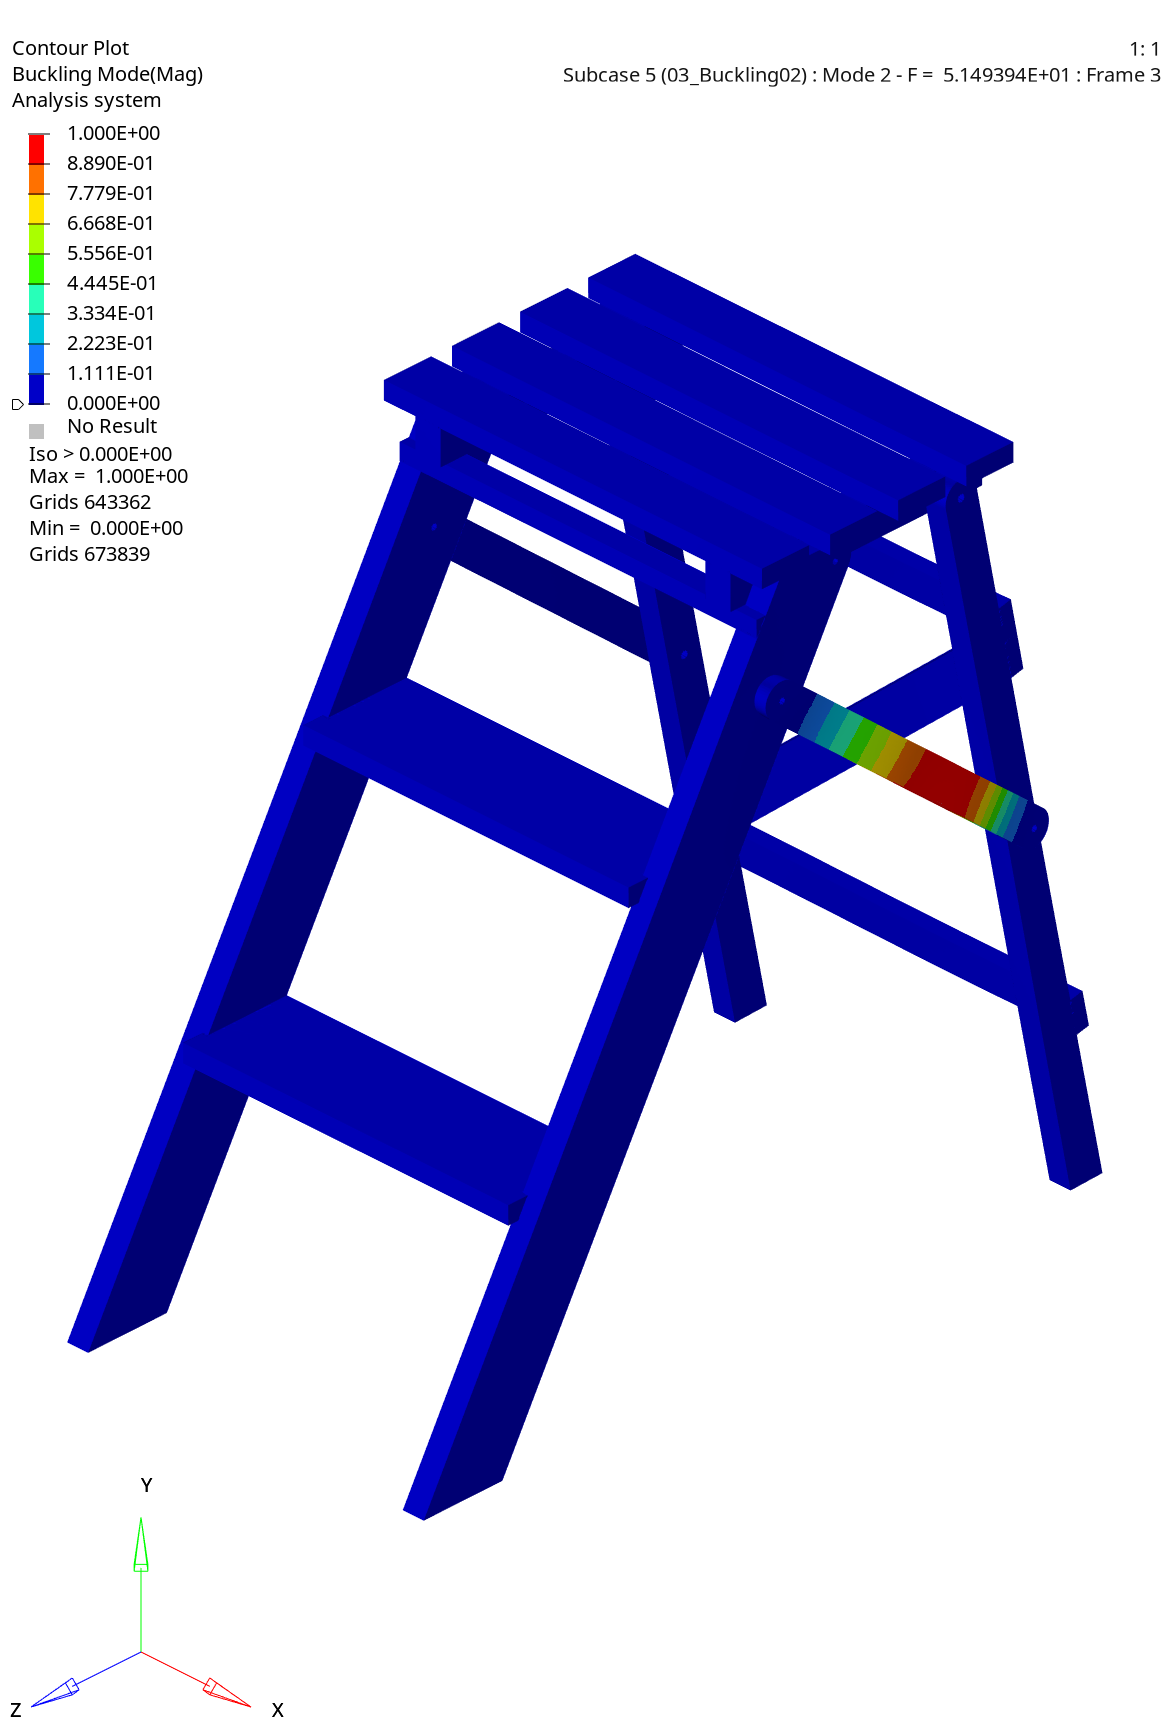
\includegraphics[width=0.48\linewidth]{pics/C030104.png}
    \captionsetup{labelformat=empty}
    \caption{\small{附图3: 稳定性分析 - 工况一、二前两阶模态输出}}
    \vspace{-0.4cm}
\end{figure}
\newpage{}
\par{}
\begin{figure}[h]
    \centering
    \vspace{-0.1cm}
    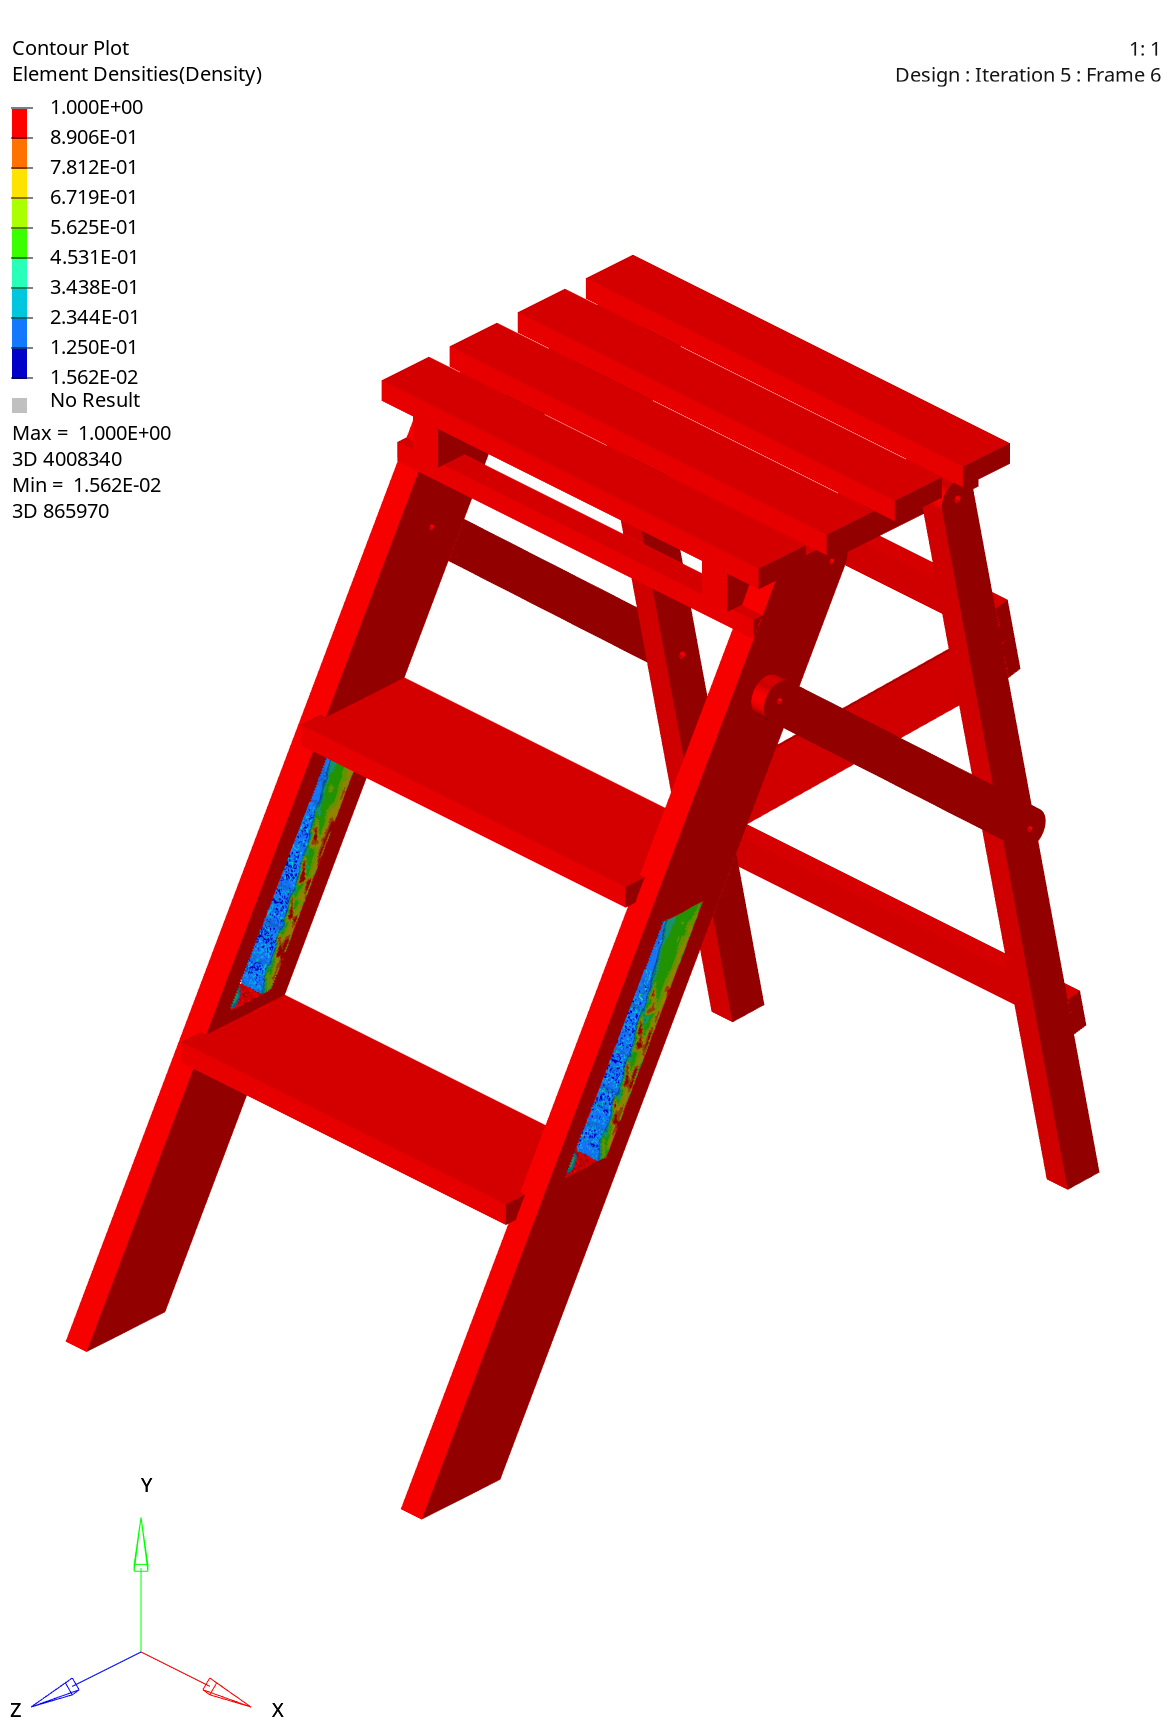
\includegraphics[width=0.48\linewidth]{pics/C040101.png}
    \\
    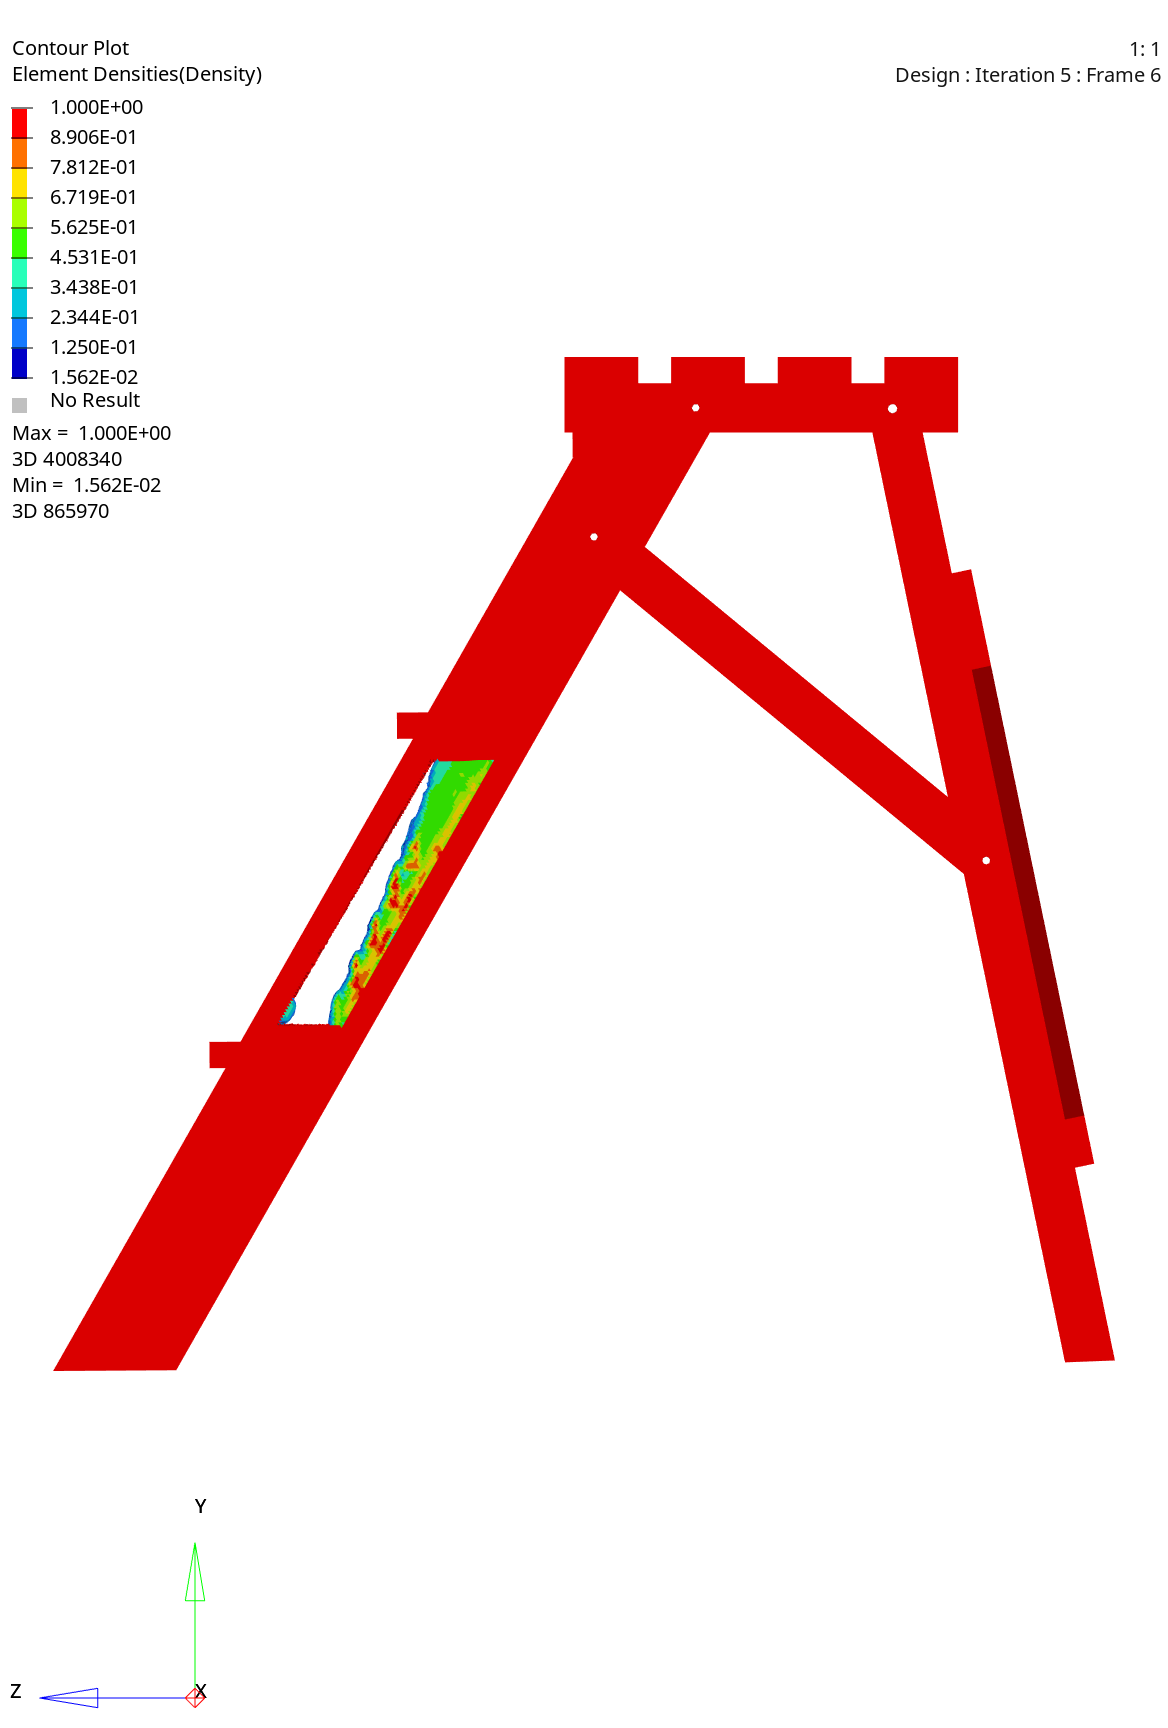
\includegraphics[width=0.48\linewidth]{pics/C040103.png}
    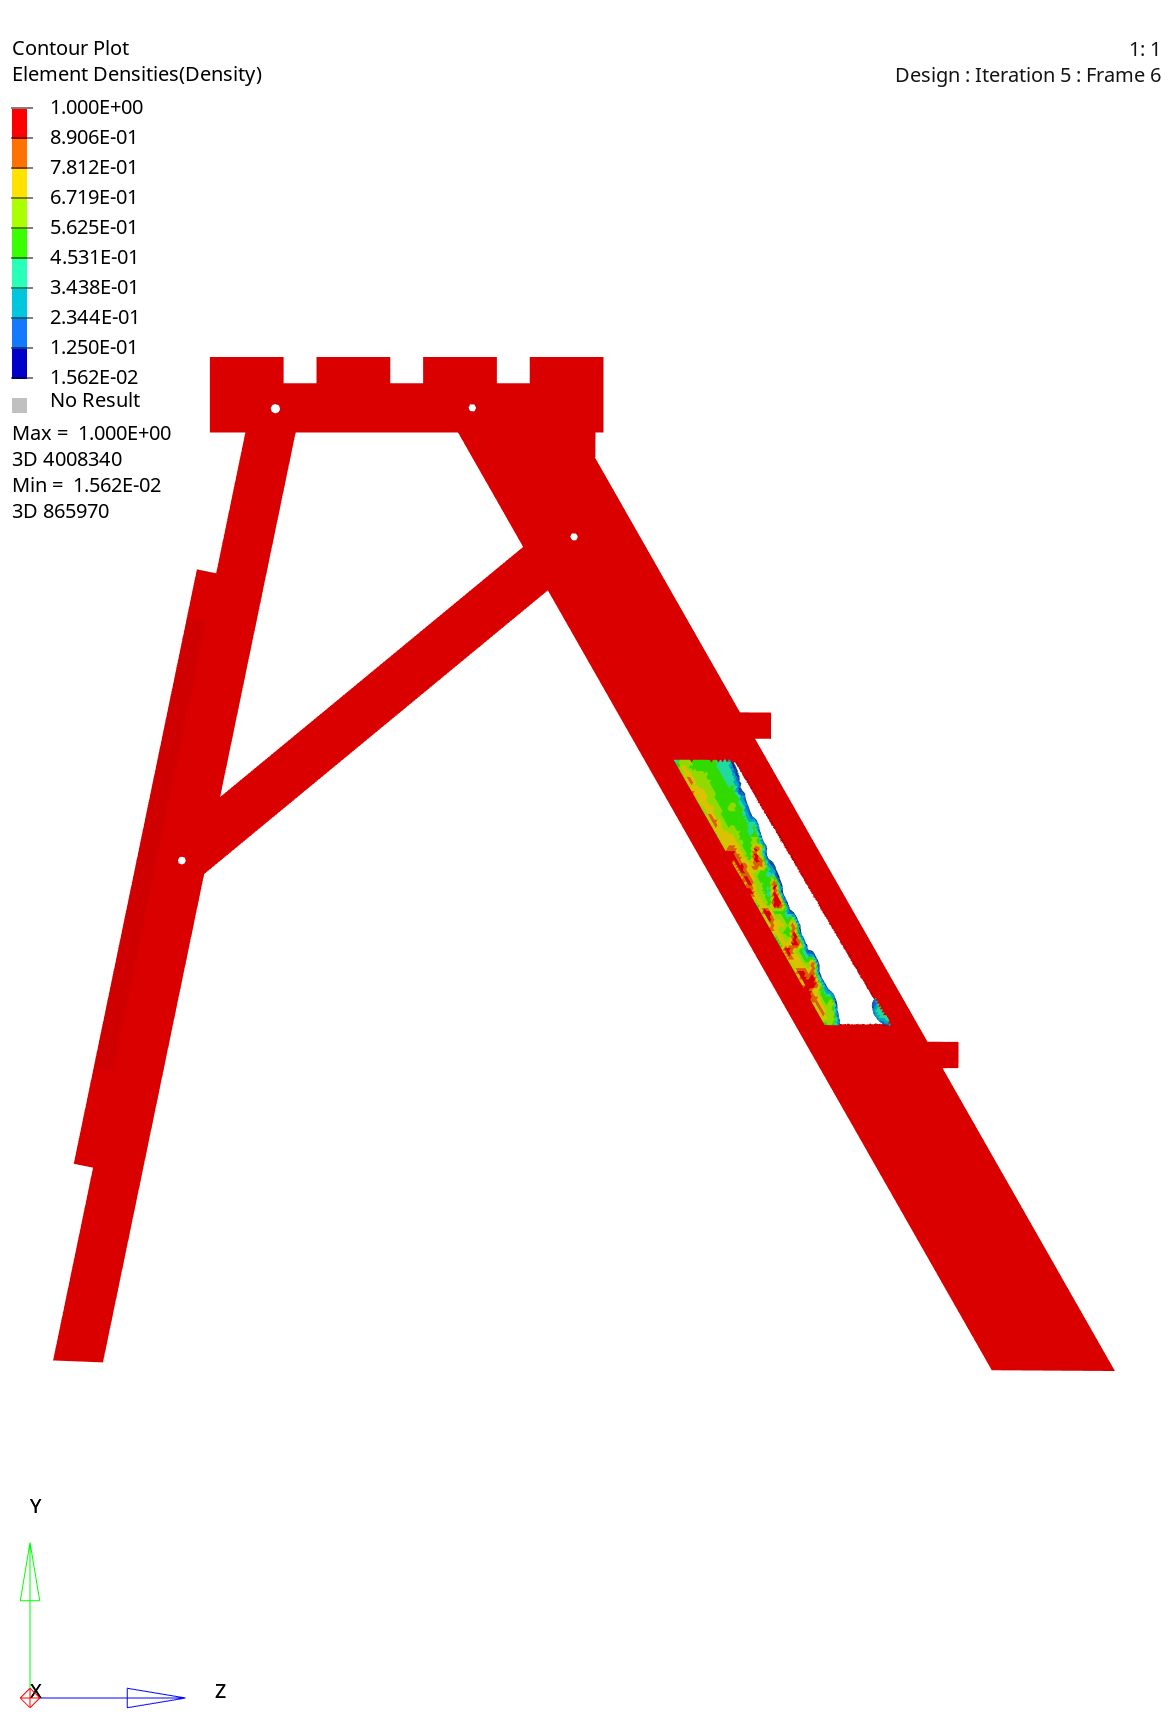
\includegraphics[width=0.48\linewidth]{pics/C040104.png}
    \captionsetup{labelformat=empty}
    \caption{\small{附图4: 结构优化分析结果输出}}
    \vspace{-0.4cm}
\end{figure}
\newpage{}
\par{}
\begin{figure}[h]
    \centering
    \vspace{-0.1cm}
    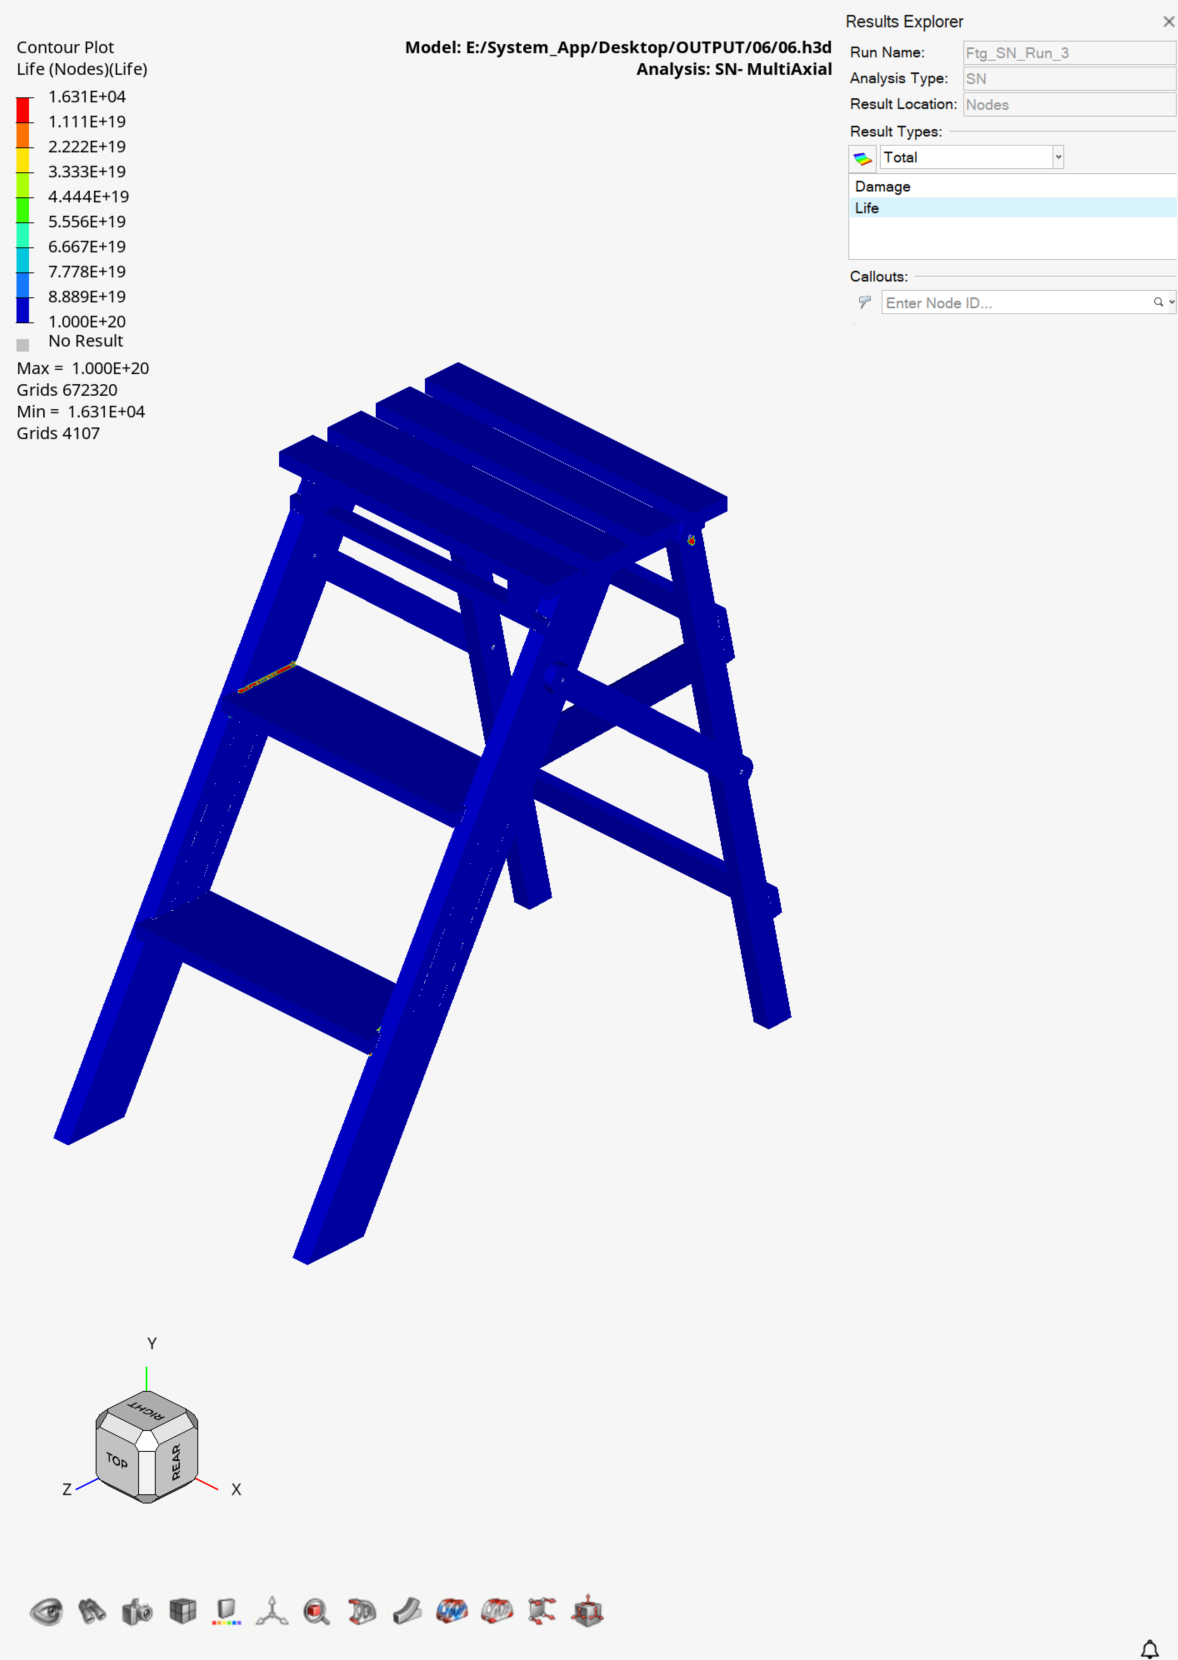
\includegraphics[width=0.48\linewidth]{pics/C050101.png}
    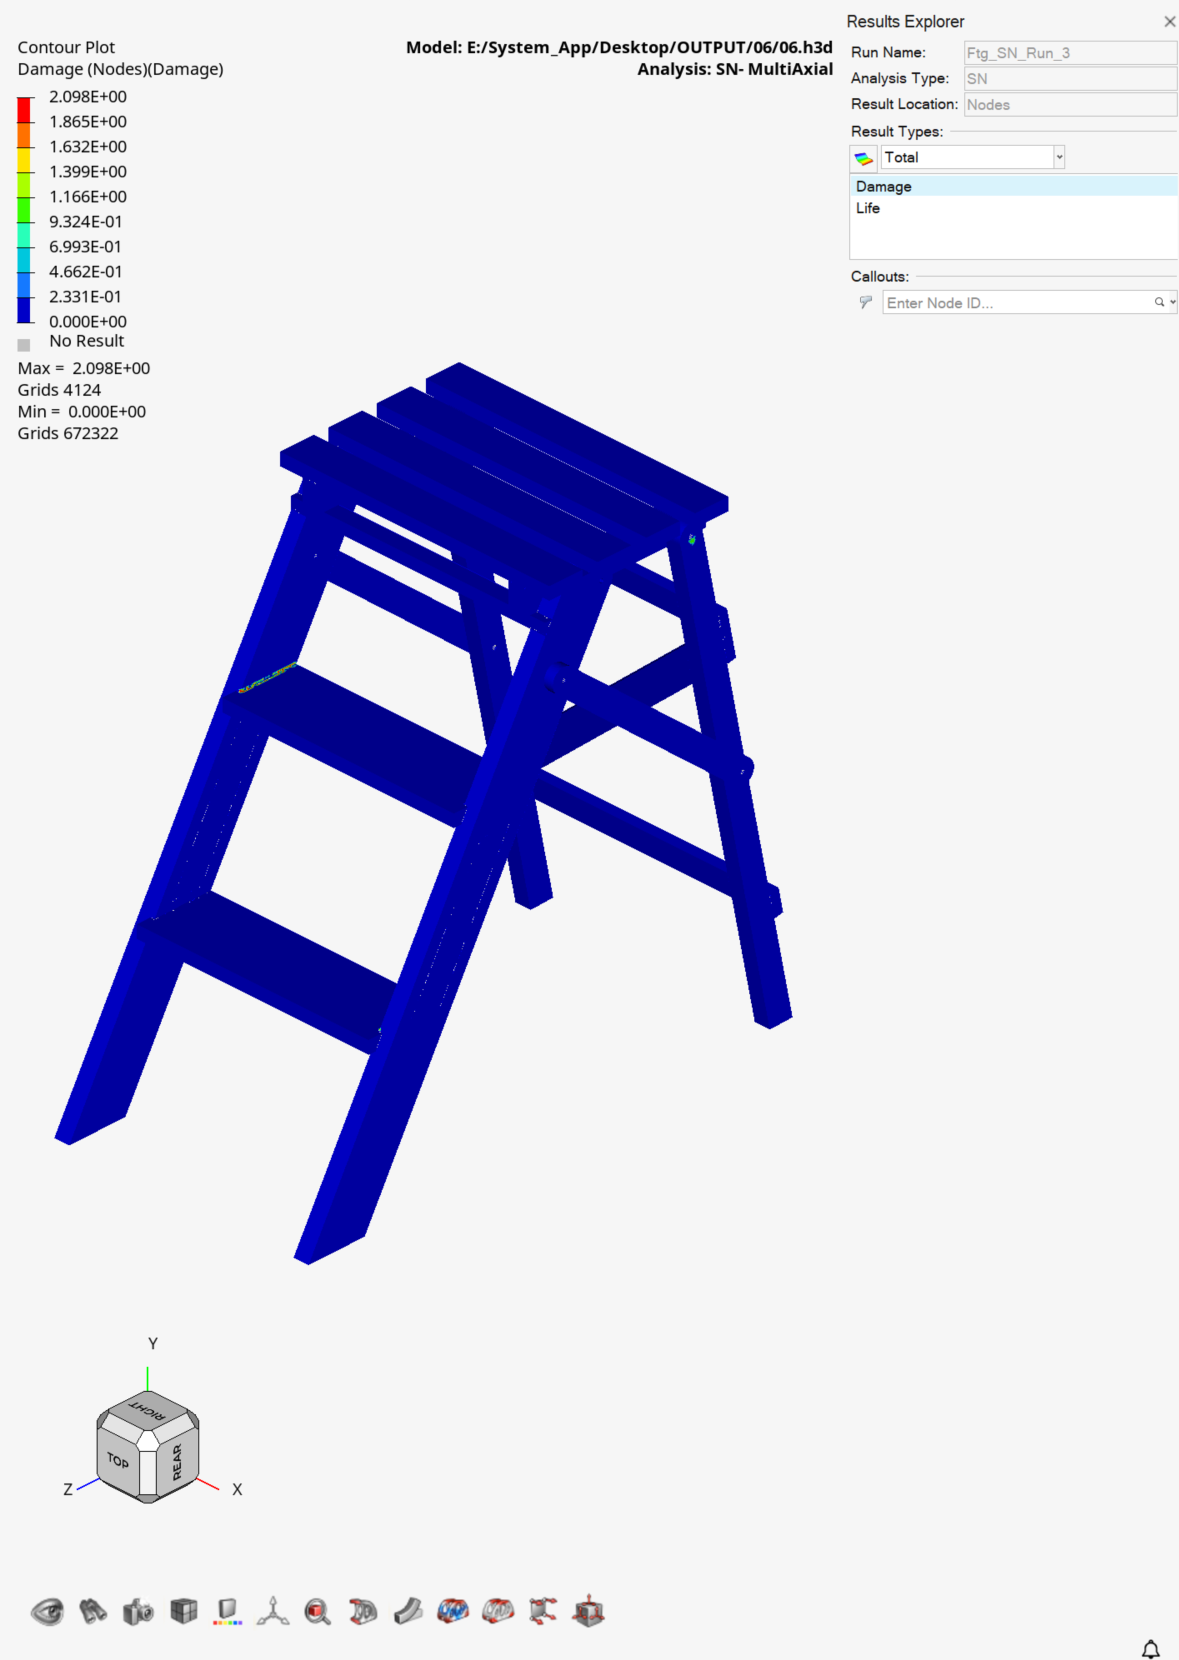
\includegraphics[width=0.48\linewidth]{pics/C050102.png}
    \captionsetup{labelformat=empty}
    \caption{\small{附图5: 疲劳分析结果输出}}
    \vspace{-0.4cm}
\end{figure}
\newpage{}
\par{}
\begin{figure}[h]
    \centering
    \vspace{-0.1cm}
    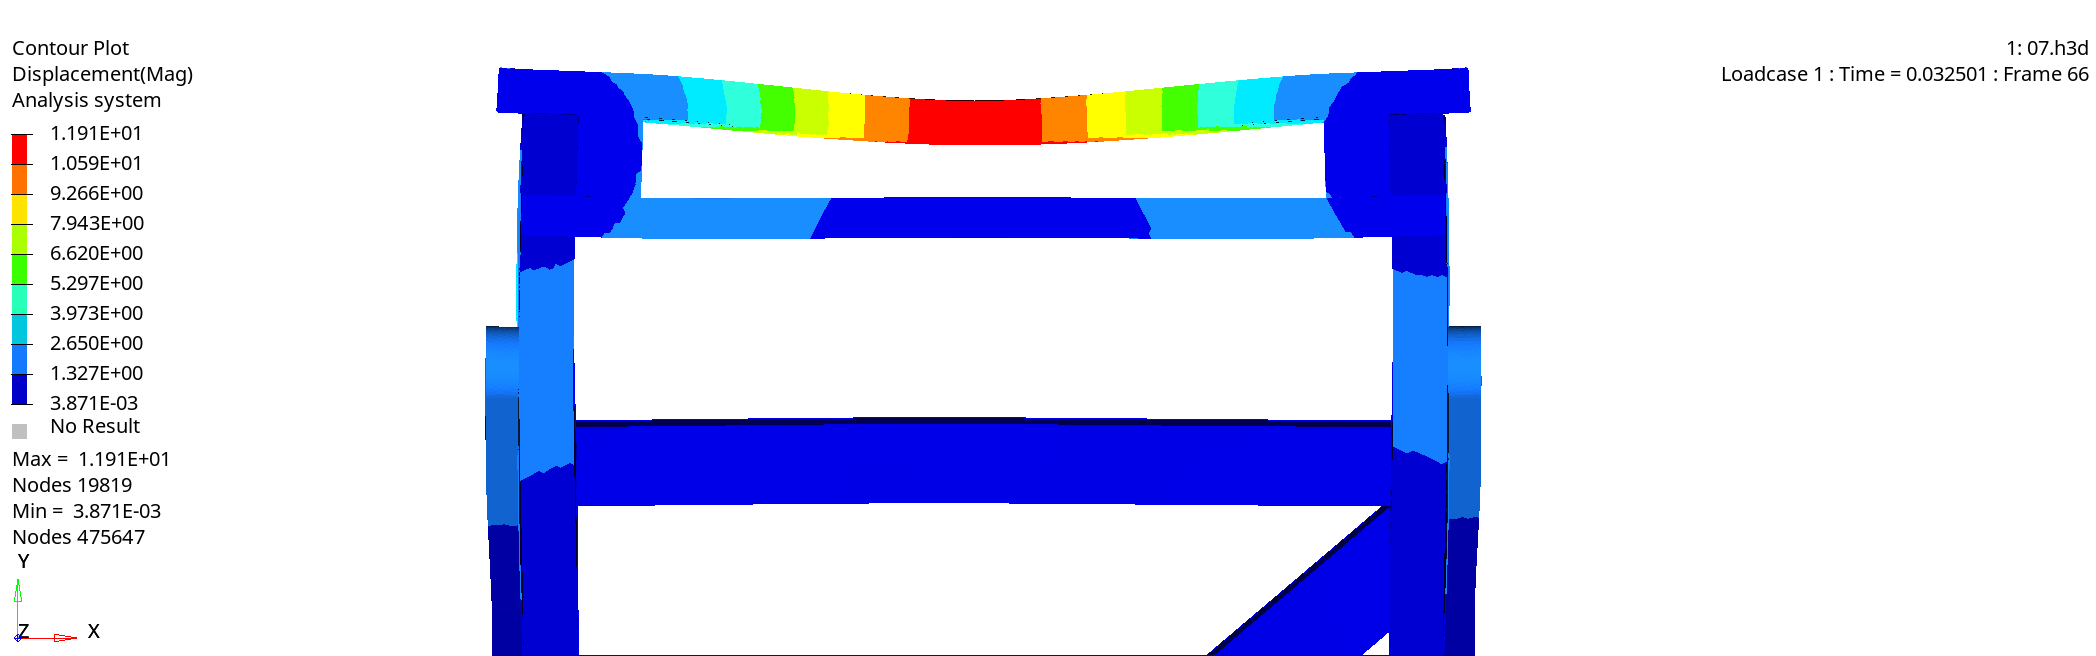
\includegraphics[width=\linewidth]{pics/C060101.png}
    \\
    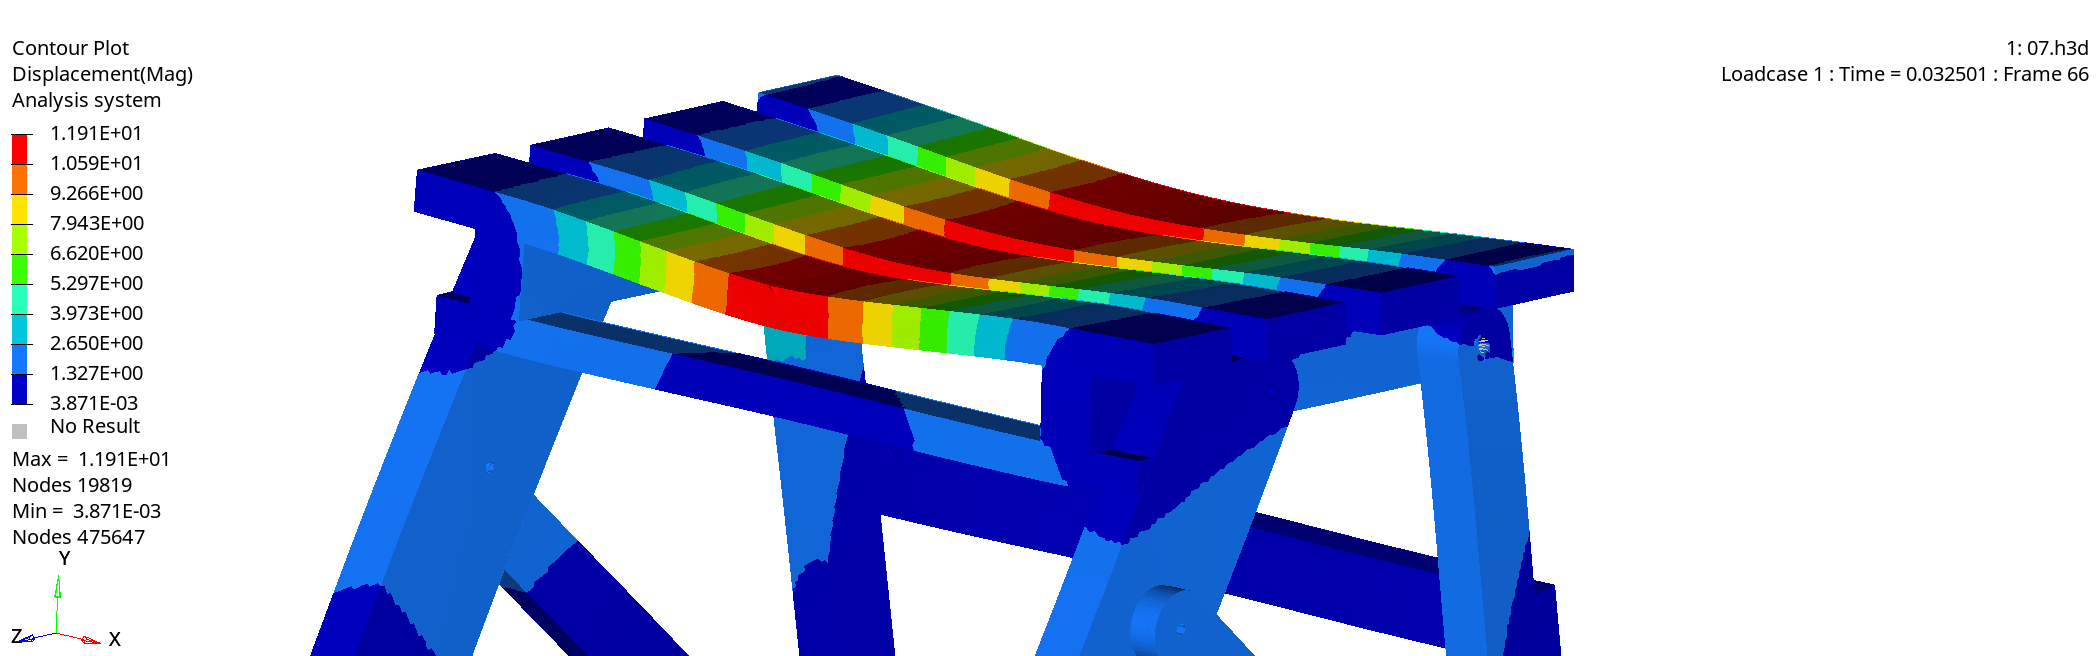
\includegraphics[width=\linewidth]{pics/C060102.png}
    \\
    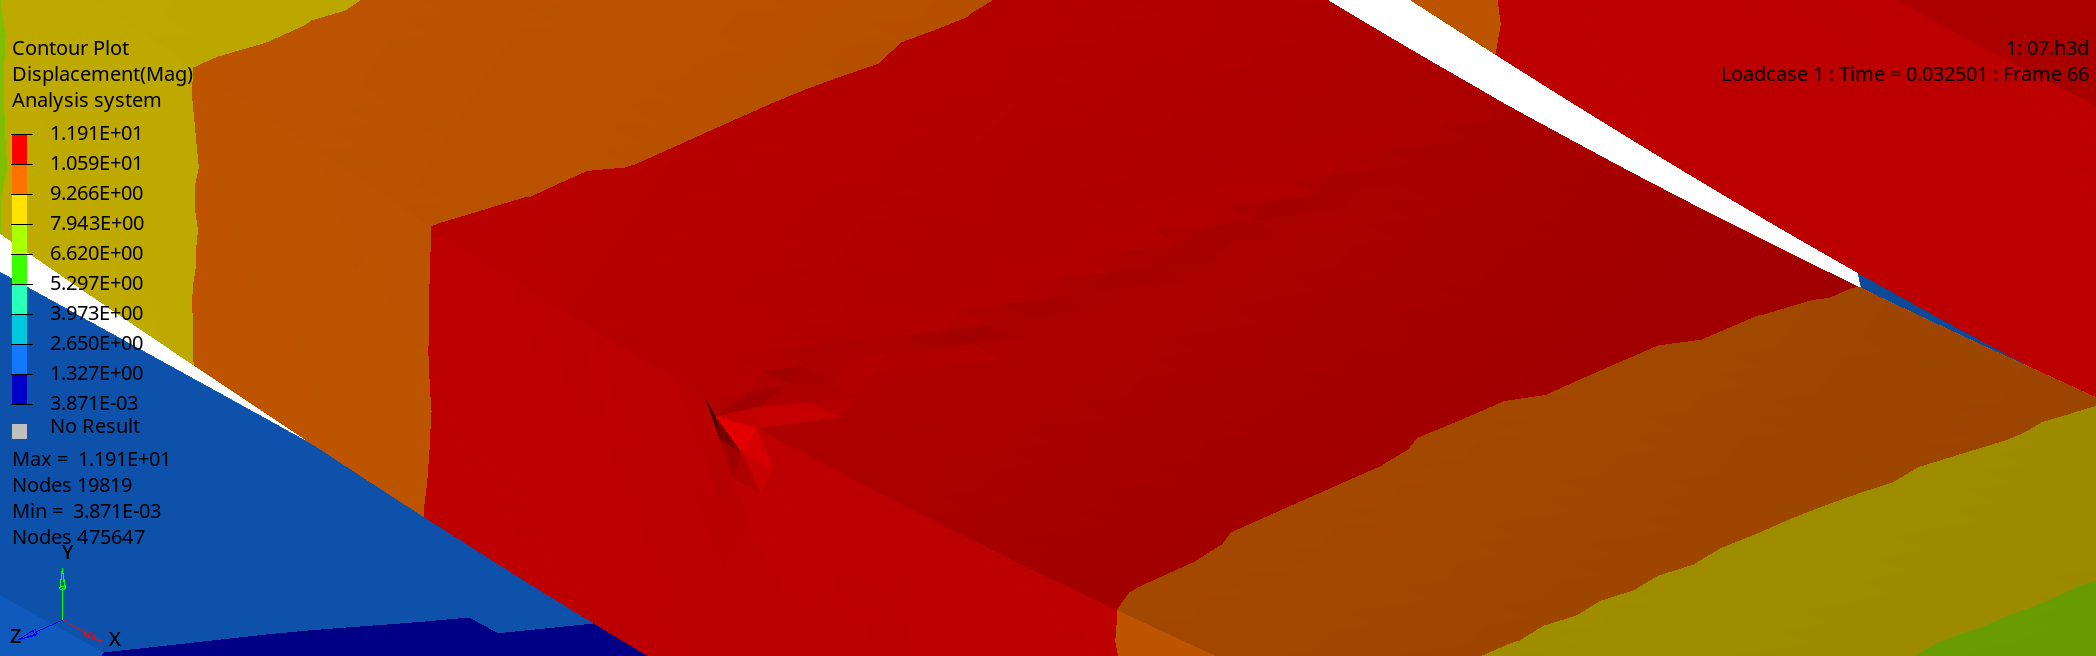
\includegraphics[width=\linewidth]{pics/C060103.png}
    \\
    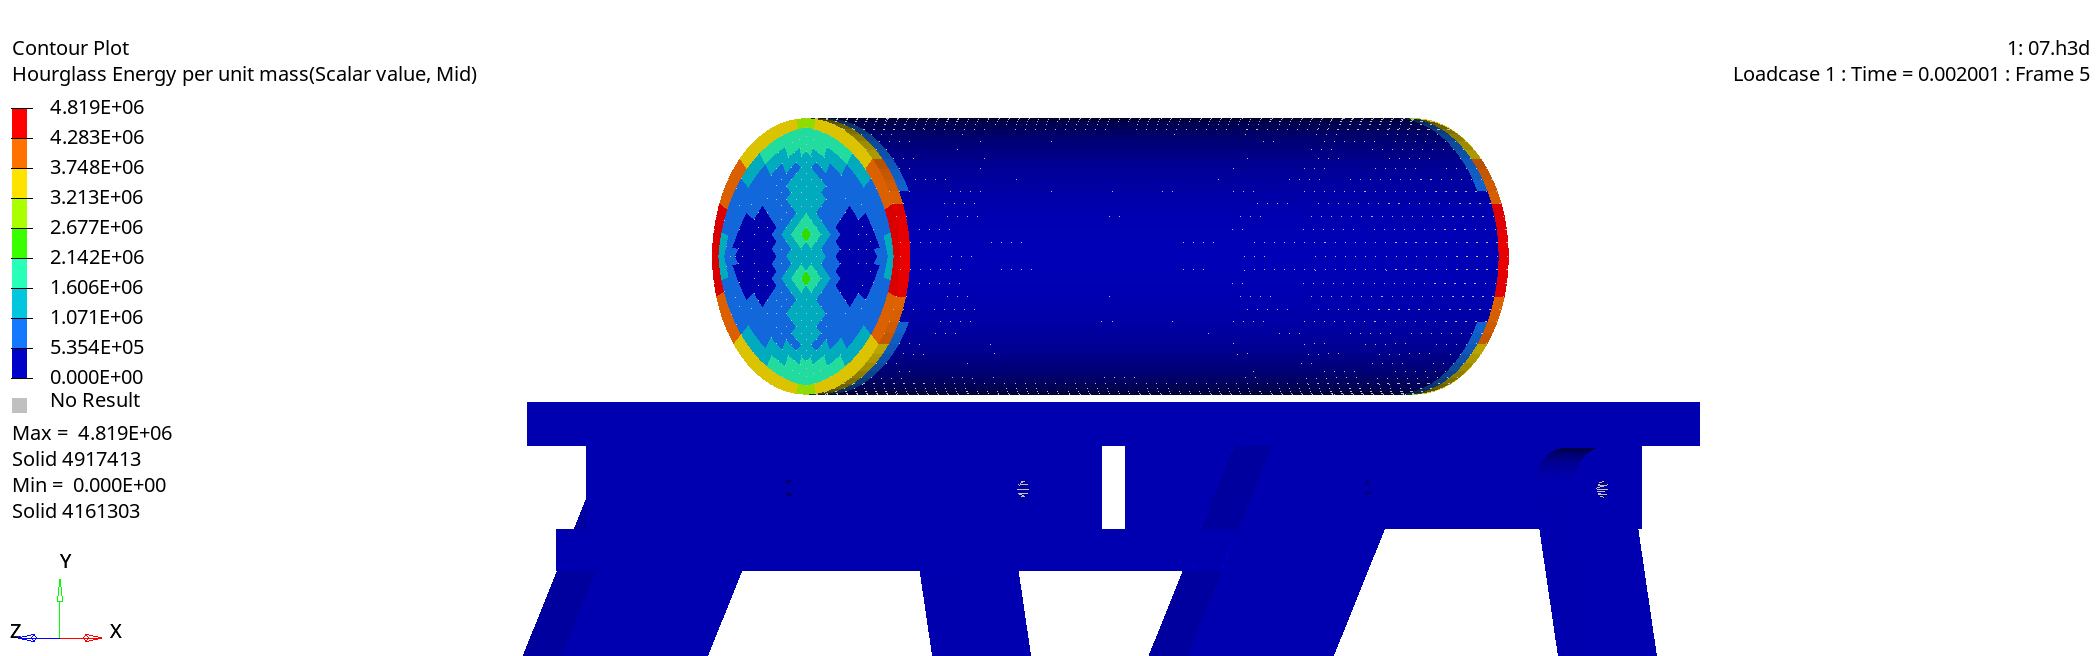
\includegraphics[width=\linewidth]{pics/C060104.png}
    \\
    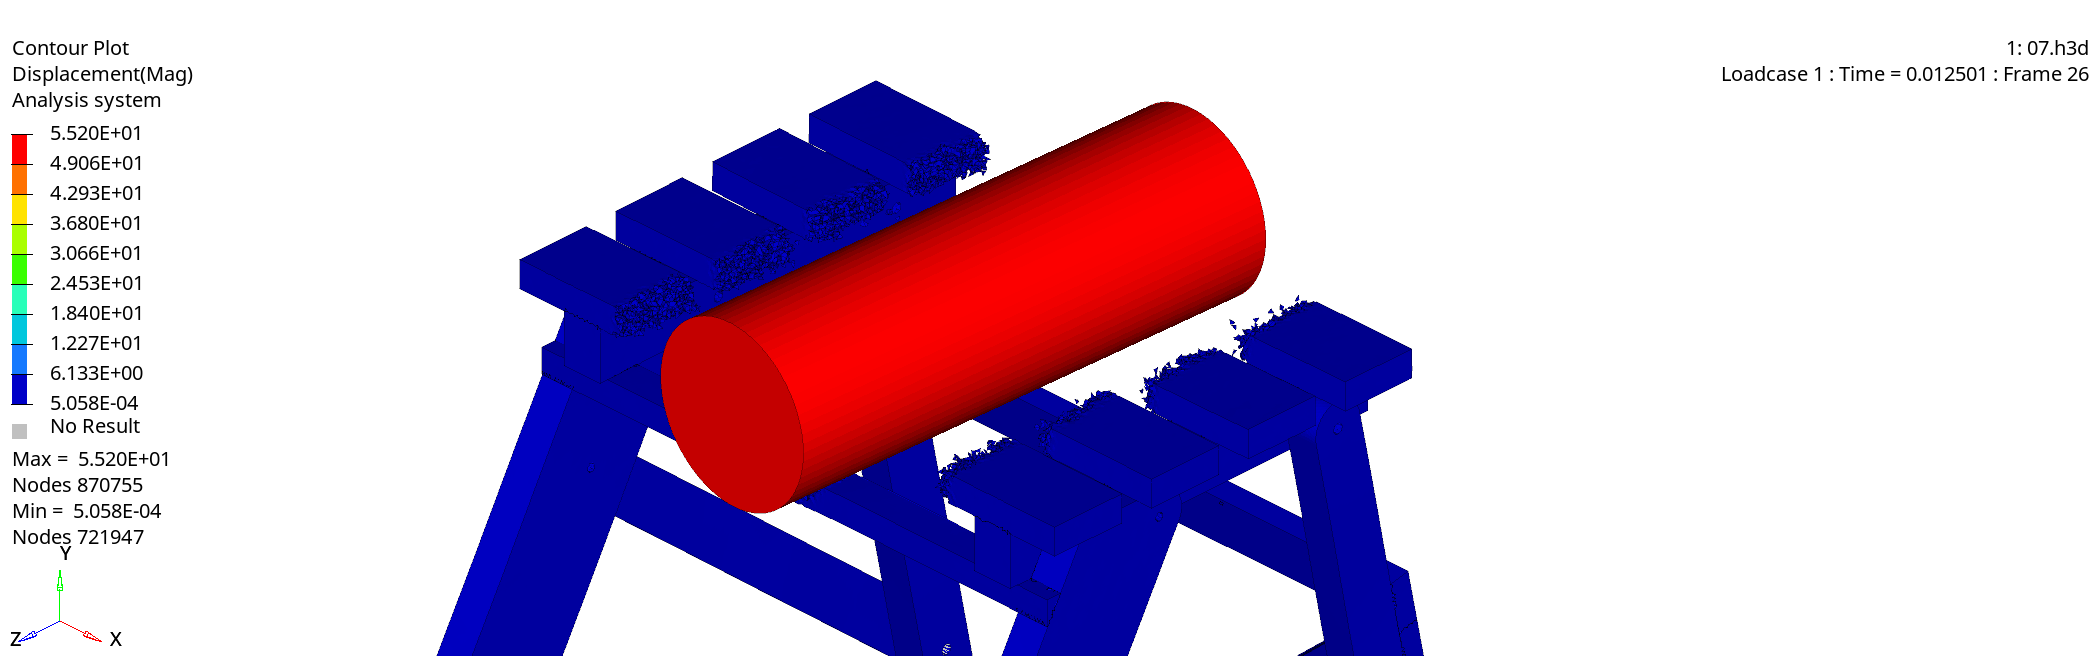
\includegraphics[width=\linewidth]{pics/C060105.png}
    \captionsetup{labelformat=empty}
    \caption{\small{附图6: 冲击耐碰撞分析结果输出}}
    \vspace{-0.4cm}
\end{figure}



\end{document}